% For book printing, change to:
% \documentclass[11pt,twoside]{report}
\documentclass[11pt]{report}

\usepackage{suthesis-2e-mod}

%% draw grid on page, useful for debugging margins
%\usepackage{pagegrid}
%\pagegridsetup{top-left,step=.5in}

\usepackage{epsfig}
\usepackage[hyphens]{url}
\usepackage{paralist}     % provides \compactitem
\usepackage{times}        % use times font
\usepackage{comment}      % provide \begin{comment}...\end{comment}
\usepackage{xcolor}       % commands for changing colors
\usepackage{lastpage}     % for total number of pages
\usepackage[normalem]{ulem} % for \sout{to strike out text}
\usepackage{stfloats}     % something to do with placement of
                          % two-column tables
\usepackage{etoolbox}     % for conditional toggles
\usepackage[pdfauthor={Diego Ongaro},
            pdftitle={Consensus: Bridging Theory and Practice},
            pdfsubject={Stanford University Ph.D. Dissertation},
            pagebackref,colorlinks=true,
            linkcolor=blue!50!black!90,
            citecolor=blue!50!black!90,
            urlcolor=blue!50!black!90,
            bookmarks]{hyperref}     % for clickable links in PDF
\usepackage{multicol}
\usepackage{tabularx}     % for easier tables with wrapped text
\usepackage{tabulary}     % for easier tables with wrapped text
\usepackage{relsize}      % for \mathlarger
\usepackage{amssymb}
\usepackage{amsmath}      % Needed to enable unnumbered equations (\begin{equation*})

\usepackage{placeins}     % provides \FloatBarrier
\usepackage{siunitx}      % typesetting units after numbers
\sisetup{range-phrase=--,
         range-units=single,
         binary-units,
         input-decimal-markers=.,
         group-separator={,},
         group-minimum-digits=4}
\usepackage{mathptmx}     % use times in math mode
\frenchspacing

\usepackage{caption}

% make links black for book printing
\ifbool{@twoside}{\hypersetup{hidelinks}}{}

% for subfigure environment, where refs look like Figure 9.8(c)
\usepackage[labelformat=simple]{subcaption}
\renewcommand\thesubfigure{(\alph{subfigure})}

\newcommand\mazieres{Mazi\`{e}res}

\title{Consensus: Bridging Theory and Practice}
\author{Diego Ongaro}
\principaladviser{John Ousterhout}
\firstreader{Mendel Rosenblum}
\secondreader{David \mazieres}
\submitdate{August 2014}

\def\thesiscopyrightpage{%
\urlstyle{same}
\null\vfill
\begin{center}
\large \copyright\ 2014 Diego Ongaro
\vspace{.75in}\\
\parbox{1.5in}{
\includegraphics[scale=1]{cc-by}
}
\parbox{3.5in}{
This work is licensed under the Creative Commons \\
Attribution 4.0 International License.\\
\url{http://creativecommons.org/licenses/by/4.0/}
}

\vspace{.75in}
\parbox{5.5in}{
This dissertation expands on a paper written by Diego Ongaro and John
Ousterhout entitled \emph{In Search of an Understandable Consensus
Algorithm}~\cite{raftatc}. Most of the paper's content is included in
some form in this dissertation. It is reproduced in this dissertation
and licensed under the Creative Commons Attribution license with
permission from John Ousterhout.
}

\vspace{1in}
This dissertation is distributed by Stanford University online:
\url{http://purl.stanford.edu/qr033xr6097}\\
The \LaTeX{} source files used to create this document are
available online:
\url{https://github.com/ongardie/dissertation/}

\end{center}
\vfill\newpage\urlstyle{tt}}

\long\def\signature#1{%
\begin{flushright}
\begin{minipage}{5in}
\parindent=0pt
I certify that I have read this dissertation and that, in my opinion,
it is fully adequate in scope and quality as a dissertation for the degree
of Doctor of Philosophy.
\par
\vspace{3ex}
\hbox to 5in{\hfil\begin{tabular}{@{}l@{}}\textbf{#1}\end{tabular}}
\end{minipage}
\end{flushright}}

\long\def\ucgssignature#1{%
\begin{flushright}
\begin{minipage}{5in}
\parindent=0pt
Approved for the Stanford University Committee on Graduate Studies.
\par
\vspace{3ex}
\hbox to 5in{\hfil\begin{tabular}{@{}l@{}}\textbf{#1}\end{tabular}}
\end{minipage}
\end{flushright}}

\def\signaturepage{%
\signature{John Ousterhout, Principal Adviser}
\vspace{.5in}
\signature{Mendel Rosenblum}
\vspace{.5in}
\signature{David \mazieres}
\vspace{.5in}
\ucgssignature{Patricia J. Gumport, Vice Provost for Graduate Education}
\vfill
\begin{center}
\emph{This signature page was generated electronically. An original signed
hard\\ copy of the signature page is on file in Stanford University
Archives.}
\end{center}
}


\newcommand\name{Raft}

\newcommand\red[1]{\textcolor{red}{#1}}   % For newly proposed text
\newcommand\redstrike[1]{\red{\sout{#1}}} % To strike out text
\newcommand\blue[1]{\textcolor{blue}{XXX- #1}} % For comments

\newcommand{\Ex}{\mathop{\bf E\/}} % expected value


\hyphenation{LogCabin} % force no hyphens in 'LogCabin'
\hyphenation{RAMCloud} % force no hyphens in 'RAMCloud'
\hyphenation{LevelDB} % force no hyphens in 'LevelDB'
\hyphenation{Append-Entries} % break 'AppendEntries' between words
\hyphenation{Request-Vote} % break 'RequestVote' between words

% Adjust caption display: bold figure name, slight margins
\usepackage{caption}
\captionsetup{labelfont=bf, margin=10pt}

% Spacing between footnotes and text.
\setlength{\skip\footins}{6ex}

% Footnotes with no number.
\makeatletter
\def\blfootnoteindented{\xdef\@thefnmark{}\@footnotetext}
\newcommand\blfootnote[1]{\blfootnoteindented{\hspace{-2.1em} #1}}
\makeatother

% read environment variables
\usepackage{catchfile}
\newcommand{\getenv}[2][]{%
  \CatchFileEdef{\temp}{"|kpsewhich --var-value #2"}{}%
  \if\relax\detokenize{#1}\relax\temp\else\let#1\temp\fi}

% Trim margins if TRIM environment variable is set to "yes".
\getenv[\TRIM]{TRIM}
\edef\trimdef{{\TRIM}}
\expandafter\ifstrequal\trimdef{yes }{
\usepackage[paperwidth=6.6in, paperheight=9.35in, top=.75in, bottom=.5in, left=.3in, right=.3in]{geometry}
}{
}

% for proof
\usepackage{color}
\definecolor{boxshade}{gray}{0.85}
\usepackage{proof/tlatex}
\usepackage{amsthm}
\theoremstyle{definition}
\newtheorem{theorem}{Theorem}
\newtheorem{definition}{Definition}
\newtheorem{lemma}{Lemma}
\newenvironment{sketch}
    {\begin{proof}[Sketch]}
    {\phantom{\qedhere}\end{proof}}
\newenvironment{assertion}
    {\begin{proof}[Assertion]}
    {\phantom{\qedhere}\end{proof}}

\newcommand\fn[1]{\textsc{#1}}
\newcommand\tab{\ \ \ \ }

\newcommand\sland{\ \land\ }
\newcommand\slor{\ \lor\ }

\newcommand\ctrl[1]{\mbox{\textbf{#1}}}
\newcommand\cif{\ctrl{if }}
\newcommand\cthen{\ctrl{ then}}
\newcommand\celse{\ctrl{else}}
\newcommand\celif{\ctrl{elif }}
\newcommand\clet{\ctrl{let }}
\newcommand\cin{\ctrl{ in}}
\newcommand\cforall{\ctrl{for all }}
\newcommand\cdo{\ctrl{ do}}

\newcommand\msg[1]{\textsc{#1}}
\newcommand\ClientRequest{\msg{ClientRequest}}
\newcommand\ClientResponse{\msg{ClientResponse}}
\newcommand\RequestVoteRequest{\msg{RequestVoteRequest}}
\newcommand\RequestVoteResponse{\msg{RequestVoteResponse}}
\newcommand\AppendEntriesRequest{\msg{AppendEntriesRequest}}
\newcommand\AppendEntriesResponse{\msg{AppendEntriesResponse}}

\newcommand\dec[1]{\mathcal{#1}}
\newcommand\messages{\dec{M}}
\newcommand\replicas{\dec{R}}
\newcommand\peers{\replicas - \{i\}}
\newcommand\ppeers{(\replicas - \{i\})}
\newcommand\operations{\dec{O}}
\newcommand\clients{\dec{C}}
\newcommand\indexes{\dec{I}}
\newcommand\terms{\dec{T}}
\newcommand\seqs{\dec{S}}
\newcommand\values{\dec{V}}
\newcommand\power{\dec{P}}
\newcommand\g{\dec{G}}
\newcommand\booleans{\dec{B}}

\newcommand\st[1]{\textsc{#1}}
\newcommand\follower{\st{follower}}
\newcommand\candidate{\st{candidate}}
\newcommand\leader{\st{leader}}

\newcommand\startfn{\tab\=\+Precondition: \=\+\kill}
\newcommand\precond{\<Precondition:\>}
\newcommand\effects{\<Effect:\>}

\newcommand\is{\triangleq}
\newcommand\be{\is}
\newcommand\domain{\mbox{DOMAIN }}
\newcommand\cat{\ \|\ }



% drop capitalization on List of Tables, List of Figures
\renewcommand{\listfigurename}{List of figures}
\renewcommand{\listtablename}{List of tables}


\begin{document}

\beforepreface

\prefacesection{Abstract}

Distributed consensus is fundamental to building fault-tolerant systems.
It allows a collection of machines to work as a coherent group that can
survive the failures of some of its members. Unfortunately, the most
common consensus algorithm, Paxos, is widely regarded as difficult to
understand and implement correctly.

This dissertation presents a new consensus algorithm called Raft, which
was designed for understandability. Raft first elects a server as leader,
then concentrates all decision-making onto the leader. These two basic
steps are relatively independent and form a better structure than Paxos,
whose components are hard to separate. Raft elects a leader using voting
and randomized timeouts. The election guarantees that the leader already
stores all the information it needs, so data only flows outwards
from the leader to other servers. Compared to other leader-based
algorithms, this reduces mechanism and simplifies the behavior. Once a
leader is elected, it manages a replicated log. Raft leverages a simple
invariant on how logs grow to reduce the algorithm's state space and
accomplish this task with minimal mechanism.

Raft is also more suitable than previous algorithms for real-world
implementations. It performs well enough for practical deployments, and
it addresses all aspects of building a complete system, including how to
manage client interactions, how to change the cluster membership, and
how to compact the log when it grows too large. To change the cluster
membership, Raft allows adding or removing one server at a time (complex
changes can be composed from these basic steps), and the cluster
continues servicing requests throughout the change.

We believe that Raft is superior to Paxos and other consensus
algorithms, both for educational purposes and as a foundation for
implementation. Results from a user study demonstrate that Raft is
easier for students to learn than Paxos. The algorithm has been formally
specified and proven, its leader election algorithm
works well in a variety of environments, and its performance is
equivalent to Multi-Paxos. Many implementations of Raft are now
available, and several companies are deploying Raft.


\prefacesection{Preface}

Readers may want to refer to the Raft website~\cite{implementations} for
videos about Raft and an interactive visualization of Raft.

\prefacesection{Acknowledgments}

Thanks to my family and friends for supporting me throughout the ups and
downs of grad school. Mom, thanks for continuously pushing me to do well
academically, even when I didn't see the point. I still don't know how
you got me out of bed at 6~a.m.\ all those mornings. Dad, thanks for
helping us earn these six (seven?) degrees, and I hope we've made you proud.
Zeide, I wish I could give
you a copy of this small book for your collection. Ernesto, thanks for
sparking my interest in computers; I still think they're pretty cool.
Laura, I'll let you know if and when I discover a RAMCloud. Thanks for
listening to hours of my drama, even when you didn't understand the
nouns. Jenny, thanks for helping me get through the drudgery of writing
this dissertation and for making me smile the whole way through. You're
crazy for having wanted to read this, and you're weird for having
enjoyed it.

I learned a ton from my many labmates, both in RAMCloud and in SCS.
Deian, I don't know why you always cared about my work; I never
understood your passion for that IFC nonsense, but keep simplifying it
until us mortals can use it. Ankita, you've single-handedly increased
the lab's average self-esteem and optimism by at least 20\%. I've
watched you learn so much already; keep absorbing it all, and I hope
you're able to see how far you've come. Good luck with your role as the
new Senior Student. Thanks especially to Ryan and Steve, with whom I
formed the first generation of RAMCloud students. Ryan, believe it or
not, your optimism helped. You were always excited about wacky ideas,
and I always looked forward to swapping CSBs (``cool story, bro'') with
you. You'll make a great advisor. Steve, I miss your intolerance for
bullshit, and I strive to match your standards for your own engineering
work. You continuously shocked the rest of us with those silent bursts
of productivity, where you'd get quarter-long projects done over a
single weekend. You guys also figured out all the program requirements
before I did and told me all the tricks. I continue to follow your lead
even after you've moved on. (Ryan, you incorrectly used the British
spelling ``acknowledgements'' rather than the American
``acknowledgments''. Steve, you did too, but you're just Canadian, not
wrong.)

Thanks to the many professors who have advised me along the way. John
Ousterhout, my Ph.D.\ advisor, should be a coauthor on this dissertation
(but I don't think they would give me a degree that way). I have never
learned as much professionally from any other person. 
John teaches by setting a great example of how to
code, to evaluate, to design, to think, and to write \emph{well}.
I have never quite
been on David \mazieres{}'s same wavelength; he's usually
\SIrange{10}{30}{minutes}
ahead in conversation. As soon as I could almost keep up with him
regarding consensus, he moved on to harder Byzantine consensus problems.
Nevertheless, David has looked out for me throughout my years in grad
school, and I've picked up some of his passion for building useful
systems and, more importantly, having fun doing so.
Mendel Rosenblum carries intimate knowledge of low level details like
x86 instruction set, yet also manages to keep track of the big
picture. He's helped me with both over the years, surprising me
with how quickly he can solve my technical problems and how clear my
predicaments are when put into his own words. Thanks to Christos Kozyrakis
and Stephen Weitzman for serving on my defense committee, and thanks to
Alan Cox and Scott Rixner for introducing me to research during
my undergraduate studies at Rice.

Many people contributed directly to this dissertation work.
A special thanks goes to David \mazieres{} and Ezra Hoch for each
finding a bug in earlier versions of Raft. David emailed us one night at
2:45~a.m.\ as he was reading through the Raft lecture slides for the
user study. He wrote that he found ``one thing quite hard to follow in
the slides,'' which turned out to be a major issue in Raft's safety.
Ezra found a liveness bug in membership changes. He posted to the
Raft mailing list,
``What if the following happens?''~\cite{Hoch:2014}, and described an
unfortunate series of events that could leave a cluster unable to
elect a leader. Thanks also to Hugues Evrard for finding a small
omission in the formal specification.

The user study would not have been possible without the support of
Ali Ghodsi, David Mazi\`{e}res, and the students of CS 294-91 at
Berkeley and CS 240 at Stanford.
Scott Klemmer helped us design the user study,
and Nelson Ray advised us on statistical analysis.
The Paxos slides for the user study borrowed heavily from a slide
deck originally created by Lorenzo Alvisi.

Many people provided feedback on other content in this dissertation.
In addition to my reading committee, Jennifer Wolochow provided helpful comments
on the entire dissertation.
Blake Mizerany, Xiang Li, and Yicheng Qin at CoreOS pushed
me to simplify the membership change algorithm towards
single-server changes.
Anirban Rahut from Splunk pointed out that membership changes may be
needlessly slow when a server joins with an empty log.
Laura Ongaro offered helpful feedback on the
user study chapter. Asaf Cidon helped direct me in finding the
probability of split votes during elections.
Eddie Kohler helped clarify the trade-offs in Raft's commitment rule,
and Maciej Smole\'{n}ski pointed out that because of it, if a leader
were to restart an unbounded number of times before it could mark entries
committed, its log could grow without bound (see Chapter~\ref{related}).
Alexander Shraer helped clarify how membership changes work in Zab.

Many people provided helpful feedback on the \name{} paper and user study
materials, including
Ed Bugnion,
Michael Chan,
Hugues Evrard,
Daniel Giffin,
Arjun Gopalan,
Jon Howell,
Vimalkumar Jeyakumar,
Ankita Kejriwal,
Aleksandar Kracun,
Amit Levy,
Joel Martin,
Satoshi Matsushita,
Oleg Pesok,
David Ramos,
Robbert van Renesse,
Mendel Rosenblum,
Nicolas Schiper,
Deian Stefan,
Andrew Stone,
Ryan Stutsman,
David Terei,
Stephen Yang,
Matei Zaharia,
24 anonymous conference reviewers (with duplicates),
and especially Eddie Kohler for shepherding the Raft paper.

Werner Vogels tweeted a link to an early draft of the \name{} paper,
which gave \name{} significant exposure. Ben Johnson and Patrick Van
Stee both gave early talks on \name{} at major industry conferences.

This work was supported by the Gigascale Systems Research Center and the
Multiscale Systems Center, two of six research centers funded under the Focus
Center Research Program, a Semiconductor Research Corporation program,
by STARnet, a Semiconductor Research Corporation program sponsored by MARCO
and DARPA, by the National Science Foundation under Grant No.~0963859,
and by grants from Facebook, Google, Mellanox, NEC, NetApp, SAP, and Samsung.
Diego Ongaro was supported by The Junglee Corporation Stanford Graduate
Fellowship. James Myers at Intel donated several SSDs used in
benchmarking.

\afterpreface

% Do this \afterpreface to avoid breaking tex.
% Stash chapter names in \Chaptername
\let\Chaptermark\chaptermark
\renewcommand\chaptermark[1]{
\def\Chaptername{#1}\Chaptermark{#1}
}

\newcommand{\vcaption}[2][Figure]{
  \caption[\Chaptername: #1]{#2}
}

% These terrible hacks make the chapter/appendix/bibliography name
% appear on odd-sided pages rather than the section name. I prefer this
% since some of my section names are too big to fit.
\makeatletter
\def\sectionmark#1{%
  }
\def\Chaptermark#1{%
  \markboth {\MakeUppercase{%
    \ifnum \c@secnumdepth >\m@ne
        \@chapapp\ \thechapter. \ %
    \fi
    #1}}{\MakeUppercase{%
    \ifnum \c@secnumdepth >\m@ne
        \@chapapp\ \thechapter. \ %
    \fi
    #1}}}%
\let\@mkboth\markboth
\makeatother


\newcommand\cold{$C_\text{old}$}
\newcommand\cnew{$C_\text{new}$}
\newcommand\cboth{$C_\text{old,new}$}


\chapter{Introduction}
\label{introduction}


Today's datacenter systems and applications run in highly dynamic
environments. They scale out by leveraging the resources of additional
servers, and they grow and shrink according to demand. Server and
network failures are also commonplace:
about 2--4\% of disk drives fail each year~\cite{Schroeder:2007},
servers crash about as often~\cite{Dean:2009}, and tens of network links
fail every day in modern datacenters~\cite{Gill:2011}.

As a result, systems must deal with servers coming and going during
normal operations. They must react to changes and adapt automatically within
seconds; outages that are noticeable to humans are typically not acceptable.
This is a major challenge in today's systems; failure handling,
coordination, service discovery, and configuration management are all
difficult in such dynamic environments.

Fortunately, distributed consensus can help with these challenges.
Consensus allows a collection of machines to work as a coherent group
that can survive the failures of some of its members. Within a consensus
group, failures are handled in a principled and proven way. Because
consensus groups are highly available and reliable, other system
components can use a consensus group as the foundation for their own
fault tolerance. Thus, consensus plays a key role in building reliable
large-scale software systems.

When we started this work, the need for consensus was becoming clear,
but many systems still struggled with problems that consensus could
solve. Some large-scale systems were still limited by a single
coordination server as a single point of failure (e.g.,
HDFS~\cite{Hadoop2Release,HDFSHA}). Many others included ad hoc
replication algorithms that handled failures unsafely (e.g., MongoDB and
Redis~\cite{Kingsbury:Jepsen}). New systems had few options for readily
available consensus implementations (ZooKeeper~\cite{Hunt:2010} was the
most popular), forcing systems builders to conform to one or build their
own.

Those choosing to implement consensus themselves usually turned to
Paxos~\cite{Lamport:1998, Lamport:2001}. Paxos had dominated the
discussion of consensus algorithms over the last two decades: most
implementations of consensus were based on Paxos or influenced by it,
and Paxos had become the primary vehicle used to teach students about
consensus.

Unfortunately, Paxos is quite difficult to understand, in spite of
numerous attempts to make it more approachable. Furthermore, its
architecture requires complex changes to support practical systems,
and building a complete system based on Paxos requires developing several
extensions for which the details have not been published or agreed upon. As a
result, both system builders and students struggle with Paxos.

The two other well-known consensus algorithms are Viewstamped
Replication~\cite{Oki:1988,Oki:1988t,Liskov:2012} and
Zab~\cite{Junqueira:2011}, the algorithm used in ZooKeeper. Although we
believe both of these algorithms are incidentally better in structure
that Paxos for building systems, neither has explicitly made this
argument; they were not designed with simplicity or understandability as
a primary goal. The burden of understanding and implementing these
algorithms is still too high.

Each of these consensus options was difficult to understand and
difficult to implement. Unfortunately, when the cost of implementing
consensus with proven algorithms was too high, systems builders were
left with a tough decision. They could avoid consensus altogether,
sacrificing the fault tolerance or consistency of their systems, or they
could develop their own ad hoc algorithm, often leading to
unsafe behavior. Moreover, when the cost of explaining and
understanding consensus was too high, not all instructors attempted to
teach it, and not all students succeeded in learning it. Consensus is as
fundamental as two-phase commit; ideally, as many
students should learn it (even though consensus is fundamentally more
difficult).

After struggling with Paxos ourselves, we set out to find a
new consensus algorithm that could provide a better foundation for
system building and education. Our approach was unusual in that our
primary goal was \emph{understandability}: could we define a consensus
algorithm for practical systems and describe it in a way that is
significantly easier to learn than Paxos? Furthermore, we wanted the
algorithm to facilitate the development of intuitions that are essential
for system builders. It was important not just for the algorithm to
work, but for it to be obvious why it works.

This algorithm also had to be complete enough to address all aspects of
building a practical system, and it had to perform well enough for
practical deployments. The core algorithm not only had to specify the
effects of receiving a message but also describe what \emph{should}
happen and when; these are equally important for systems builders.
Similarly, it had to guarantee consistency, and it also had to provide
availability whenever possible. It also had to address the many aspects
of a system that go beyond reaching consensus, such as changing the
members of the consensus group. These are necessary in practice, and
leaving this burden to systems builders would risk ad hoc, suboptimal,
or even incorrect solutions.

The result of this work is a consensus algorithm called Raft. In
designing Raft we applied specific techniques to improve
understandability, including decomposition (Raft separates leader
election, log replication, and safety) and state space reduction (Raft
reduces the degree of nondeterminism and the ways servers can be
inconsistent with each other). We also addressed all of the issues needed to
build a complete consensus-based system. We considered each design
choice carefully, not just for the benefit of our own implementation but
also for the many others we hope to enable.

We believe that Raft is superior to Paxos and other consensus
algorithms, both for educational purposes and as a foundation for
implementation. It is simpler and more understandable than other
algorithms; it is described completely enough to meet the needs of a
practical system; it has several open-source implementations and is used
by several companies; its safety properties have been formally specified
and proven; and its efficiency is comparable to other algorithms.

The primary contributions of this dissertation are as follows:
%
\begin{itemize}
%
\item The design, implementation, and evaluation of the Raft consensus
algorithm. Raft is similar in many ways to existing consensus algorithms
(most notably, Oki and Liskov's Viewstamped Replication~\cite{Oki:1988,
Liskov:2012}), but it is designed for understandability. This led to
several novel features. For example, Raft uses a stronger form of
leadership than other consensus algorithms.
This simplifies the management of the replicated log and makes Raft
easier to understand.
%
\item The evaluation of Raft's understandability. A user study with 43
students at two universities shows that Raft is significantly easier to
understand than Paxos: after learning both algorithms, 33 of these
students were able to answer questions about Raft better than questions
about Paxos. We believe this is the first scientific study to evaluate
consensus algorithms based on teaching and learning.
%
\item The design, implementation, and evaluation of Raft's leader
election mechanism.  While many consensus algorithms do not prescribe a
particular leader election algorithm, Raft includes a specific algorithm
involving randomized timers. This adds only a small amount of mechanism
to the heartbeats already required for any consensus algorithm, while
resolving conflicts simply and rapidly. The evaluation of leader
election investigates its behavior and performance, concluding that this simple
approach is sufficient in a wide variety of practical environments. It
typically elects a leader in under 20 times the cluster's one-way
network latency.
%
\item The design and implementation of Raft's cluster membership change
mechanism. Raft allows adding or removing a single server at a time;
these operations preserve safety simply, since at least one server
overlaps any majority during the change. More complex changes in
membership are implemented as a series of single-server changes.
Raft allows the
cluster to continue operating normally during changes, and membership
changes can be implemented with only a few extensions to the basic
consensus algorithm.
%
\item A thorough discussion and implementation of the other components
necessary for a complete consensus-based system, including client
interaction and log compaction. Although we do not believe these aspects
of Raft to be particularly novel, a complete description is important
for understandability and to enable others to build real systems. We have
implemented a complete consensus-based service to explore and address
all of the design decisions involved.
%
\item A proof of safety and formal specification for the Raft algorithm.
The level of precision in the formal specification aids in reasoning
carefully about the algorithm and clarifying details in the algorithm's
informal description. The proof of safety helps build confidence in
Raft's correctness. It also aids others who wish to extend Raft by
clarifying the implications for safety of their extensions.
%
\end{itemize}

We have implemented many of the designs in this dissertation in
an open-source implementation of Raft called LogCabin~\cite{logcabin}.
LogCabin served as our test platform for new ideas in Raft
and as a way to verify that we understood the issues of building a
complete and practical system. The implementation is described in more
detail in Chapter~\ref{performance}.

The remainder of this dissertation introduces the replicated state
machine problem and discusses the strengths and weaknesses of Paxos
(Chapter~\ref{motivation}); presents the Raft consensus algorithm, 
its extensions for cluster membership changes and log compaction, and
how clients interact with Raft
(Chapters~\ref{basicraft}--\ref{clients});
evaluates Raft for understandability, correctness, and leader election
and log replication performance
(Chapters~\ref{userstudy}--\ref{performance}); and discusses related
work (Chapter~\ref{related}).

\chapter{Motivation}
\label{motivation}

Consensus is a fundamental problem in fault-tolerant systems: how can
servers reach agreement on shared state, even in the face of failures?
This problem arises in a wide variety of systems that need to provide
high levels of availability and cannot compromise on consistency; thus,
consensus is used in virtually all consistent large-scale storage
systems. Section~\ref{motivation:problem} describes how consensus is
typically used to create replicated state machines, a general-purpose
building block for fault-tolerant systems; Section~\ref{motivation:uses}
discusses various ways replicated state machines are used in larger
systems; and Section~\ref{motivation:paxos} discusses the problems with
the Paxos consensus protocol, which Raft aims to address.

\section{Achieving fault tolerance with replicated state machines}
\label{motivation:problem}

Consensus algorithms typically arise in the context of
\emph{replicated state machines}~\cite{Schneider:1990}. In this approach, state
machines on a collection of servers compute identical copies of
the same state and can continue operating even if some of the
servers are down.
Replicated state machines are used to solve a variety of
fault tolerance problems in
distributed systems, as described in
Section~\ref{motivation:uses}.
Examples of replicated state machines include Chubby~\cite{Burrows:2006}
and ZooKeeper~\cite{Hunt:2010},
which both provide hierarchical key-value stores for small
amounts of configuration data. In addition to basic operations such as
\emph{get} and \emph{put}, they also provide synchronization primitives
like \emph{compare-and-swap}, enabling concurrent clients to coordinate
safely.

\begin{figure}
\centering
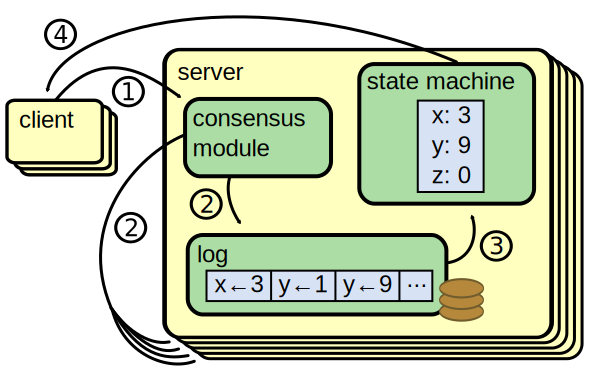
\includegraphics[scale=.50]{motivation/statemachine}
\vcaption[replicated state machine architecture]{
Replicated state machine architecture.
The consensus algorithm
manages a replicated log containing state machine commands from
clients. The state machines process identical sequences of commands
from the logs, so they produce the same outputs.}
\label{fig:motivation:statemachine}
\end{figure}

Replicated state machines are typically implemented using a replicated
log, as shown in Figure~\ref{fig:motivation:statemachine}. Each server stores a log
containing a series of commands, which its state machine executes in order.
Each log contains the same commands in the same order, so each state
machine processes the same sequence of commands. Since the state
machines are deterministic, each computes the same state and the same
sequence of outputs.

Keeping the replicated log consistent is the job of the consensus
algorithm. The consensus
module on a server receives commands from clients and adds them to its log.
It communicates with the consensus modules on other servers to
ensure that every log eventually contains
the same requests in the
same order, even if some servers fail. Once commands are properly
replicated, they are said to be \emph{committed}. Each server's state machine processes
committed commands in log order, and the outputs are returned to clients.
As a result, the servers appear to
form a single, highly reliable state machine.

Consensus algorithms for practical systems typically have the following
properties:
\begin{itemize}
\item They ensure \emph{safety} (never returning an incorrect
result) under all non-Byzantine
conditions, including network delays,
partitions, and packet loss, duplication, and reordering.
\item They are
fully functional (\emph{available}) as long as any majority of the servers are
operational and can communicate with each other and with clients.
Thus, a typical cluster of five servers can tolerate the
failure of any two servers.
Servers are assumed to fail by stopping; they may later recover from
state on stable storage and rejoin the cluster.
\item They do not depend on timing to ensure the consistency
of the logs: faulty clocks and extreme message delays can, at worst,
cause availability problems. That is, they maintain safety under an
\emph{asynchronous} model~\cite{Lynch:1996}, in
which messages and processors proceed at arbitrary speeds.
\item In the common
case, a command can complete as soon as a majority of the cluster
has responded to a single round of remote procedure calls; a minority
of slow servers need not impact overall system performance.
\end{itemize}


\section{Common use cases for replicated state machines}
\label{motivation:uses}

Replicated state machines are a general-purpose building block for making
systems fault-tolerant. They can be used in a variety of ways, and this
section discusses some typical usage patterns.

\begin{figure}
\hfill
\begin{subfigure}{.45\textwidth}
\centering
\includegraphics[scale=.5]{motivation/activeactive}
\caption{
The nodes in the cluster coordinate among themselves by reading from and
writing to the replicated state machine.
\\
}
\label{fig:motivation:activeactive}
\end{subfigure}
\hfill
\begin{subfigure}{.45\textwidth}
\centering
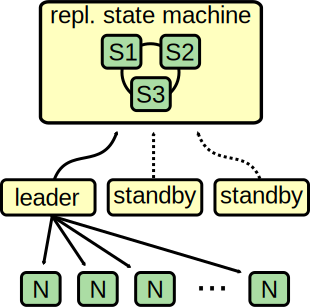
\includegraphics[scale=.5]{motivation/activepassive}
\caption{
One leader actively manages the nodes in the cluster and records its
state using the replicated state machine. Other standby servers are
passive until the leader fails.
}
\label{fig:motivation:activepassive}
\end{subfigure}
\hfill
\vcaption[common patterns for using a single replicated state machine]{
Common patterns for using a single replicated state machine.
}
\end{figure}


Most common deployments of consensus have just three or five servers
forming one replicated state machine. Other servers can then use this
state machine to coordinate their activities, as shown in
Figure~\ref{fig:motivation:activeactive}. These systems often use the
replicated state machine to provide
group membership, configuration management, or locks~\cite{Hunt:2010}.
As a more specific example, the replicated state machine could provide a
fault-tolerant work queue, and other servers could coordinate using the
replicated state machine to assign work to themselves.

A common simplification to this usage is shown in
Figure~\ref{fig:motivation:activepassive}. In this pattern, one
server acts as leader, managing the rest of the servers.
The leader stores its critical data in the consensus system.
In case it fails, other standby servers compete for the position of
leader, and if they succeed, they use the data in the consensus system
to continue operations.
Many large-scale storage systems that have a single cluster leader, such as
GFS~\cite{Ghemawat:2003}, HDFS~\cite{Shvachko:2010}, and
RAMCloud~\cite{Ousterhout:2011}, use this approach.

\begin{figure}
\centering
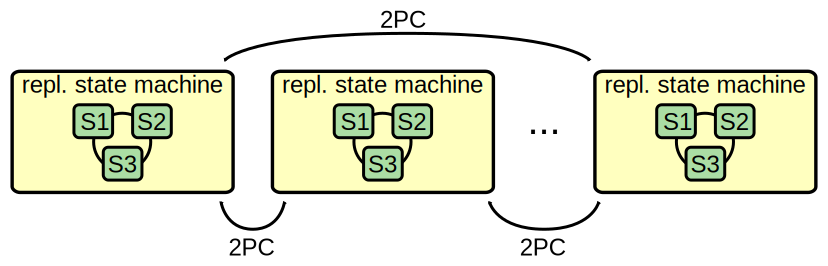
\includegraphics[scale=.5]{motivation/bigdata}
\vcaption[partitioned large-scale storage system using consensus]{
Partitioned large-scale storage system using consensus.
For scale, data is partitioned across many replicated state machines.
Operations that span partitions use a two-phase commit protocol.
}
\label{fig:motivation:bigdata}
\end{figure}

Consensus is also sometimes used to replicate very large amounts of
data, as shown in Figure~\ref{fig:motivation:bigdata}. Large storage
systems, such as Megastore~\cite{Baker:2011},
Spanner~\cite{Corbett:2012}, and Scatter~\cite{Glendenning:2011},
store too much data to fit in a single group
of servers. They partition their data across many replicated state machines,
and operations that span multiple partitions use a two-phase commit
protocol (2PC) to
maintain consistency.



\section{What's wrong with Paxos?}
\label{motivation:paxos}

\begin{figure*}
\centering
\includegraphics[scale=0.95]{motivation/paxossummary}
\vcaption[summary of the single-decree Paxos protocol]{
Summary of the single-decree Paxos consensus protocol.
See \cite{Lamport:2001} for a detailed explanation.
}
\label{fig:motivation:paxos:basic}
\end{figure*}


Over the last ten years, Leslie Lamport's Paxos protocol~\cite{Lamport:1998}
has become almost synonymous with consensus: it is the protocol
most commonly taught in courses, and most implementations of consensus
use it as a starting point. Paxos first defines a protocol capable
of reaching agreement on a single decision, such as a single replicated
log entry.  We refer to this subset as \emph{single-decree Paxos}.
Paxos then combines multiple instances of this protocol to facilitate
a series of decisions such as a log (\emph{Multi-Paxos}).
Single-decree Paxos is summarized in
Figure~\ref{fig:motivation:paxos:basic}, and Multi-Paxos is summarized
in Figure~\ref{fig:appendix:userstudy:paxossummary4}.
Paxos ensures safety and liveness (it eventually reaches consensus,
assuming an adequate failure detector
is used to avoid proposer livelock), and its correctness has been proven.
Multi-Paxos is efficient in the normal case, and Paxos supports changes
in cluster membership~\cite{Lorch:2006}.

Unfortunately, Paxos has two significant drawbacks.  The first drawback is
that Paxos is exceptionally difficult to understand. The full
explanation~\cite{Lamport:1998} is notoriously opaque; few
people succeed in understanding it, and only with great effort.
As a result, there have been several attempts to explain Paxos
in simpler terms~\cite{Lamport:2001, Lampson:1996, Lampson:2001}.
These explanations focus on the single-decree subset,
yet they are still challenging.
In an informal survey of attendees at NSDI 2012, we found few people who
were comfortable with Paxos, even among seasoned researchers.
We struggled with Paxos ourselves; we were not able to understand
the complete protocol
until after reading several explanations
and designing our own alternative protocol, a process that took
almost a year.

We hypothesize that Paxos' opaqueness stems from its choice of the
single-decree subset as its foundation. Single-decree
Paxos is dense and subtle: it is divided into two stages that do
not have simple intuitive explanations and cannot be understood
independently. Because of this, it is difficult to
develop intuitions about why the single-decree protocol works.
The composition rules for Multi-Paxos add significant additional
complexity and subtlety. We believe that the overall
problem of reaching consensus on multiple decisions (i.e., a log instead
of a single entry) can be decomposed in other ways that are more
direct and obvious.

The second problem with Paxos is that it does not provide a good
foundation
for building practical implementations. One reason is that
there is no widely agreed-upon algorithm for Multi-Paxos.
Lamport's descriptions are mostly about single-decree Paxos;
he sketched possible approaches to Multi-Paxos, but many
details are missing. There have been several attempts to flesh out and
optimize Paxos, such as \cite{Mazieres:2007}, \cite{Renesse:2011},
and \cite{Kirsch:2008},
but these differ from each other and from Lamport's sketches.
Systems such as Chubby~\cite{Chandra:2007} have implemented
Paxos-like algorithms, but in most cases their details have not been
published.


Furthermore, the Paxos
architecture is a poor one
for building practical systems; this
is another consequence of the
single-decree decomposition. For example, there is
little benefit to
choosing a collection of log entries independently and then melding
them into a sequential log; this just adds complexity.  It is simpler
and more efficient to design a system around a log, where new
entries are appended sequentially in a constrained order.
Another problem is that Paxos
uses a symmetric peer-to-peer approach at its core (though it
also suggests a weak form of leadership as a performance
optimization). This makes
sense in a simplified world where only one decision will be made,
but few practical systems use this approach. If a series of decisions
must be made, it is simpler and faster to first elect a
leader, then have the leader coordinate the decisions.
(Chapter~\ref{related} discusses Egalitarian Paxos, a recent
variant of Paxos that does not use a leader but in some situations can
be more efficient than algorithms that do; however, this algorithm is
much more complex than leader-based algorithms.)

As a result, practical systems bear little resemblance to Paxos.
Each implementation begins with Paxos, discovers the difficulties in
implementing it, and then develops a significantly different architecture.
This is time-consuming and error-prone, and the difficulties of
understanding Paxos exacerbate the problem.
Paxos' formulation may be a good one for proving theorems about
its correctness, but real implementations are so
different from Paxos that the proofs have little value. The following
comment from the Chubby implementers is typical:

{\defaultleftmargin{4em}{}{}{}
\begin{quote}
There are significant gaps between the description of the Paxos
algorithm and the needs of a real-world system\dots. the final system
will be based on an unproven protocol~\cite{Chandra:2007}.
\end{quote}
}

Because of these problems, we concluded that Paxos does not provide
a good foundation either for system building or for education.
Given the importance of consensus in large-scale software
systems, we decided to see if we could design an alternative consensus
algorithm with better properties than Paxos.  \name{} is the result
of that experiment.


%



\chapter{Basic Raft algorithm}
\label{basicraft}

This chapter presents the Raft algorithm. We designed Raft to be
as understandable as possible; the first section describes our approach
to designing for understandability. The following sections describe the
algorithm itself and include examples of design choices we made for
understandability.

\section{Designing for understandability}
\label{basicraft:understandability}

We had several goals in designing \name{}: it must provide a complete
and practical foundation for system building, so that it
significantly reduces the amount of design work required of developers;
it must be safe under all conditions and available under
typical operating conditions; and it must be efficient for
common operations. But our most important goal---and most difficult
challenge---was \emph{understandability}. It must be possible
for a large audience to understand the algorithm comfortably.
In addition, it must be possible to develop intuitions
about the algorithm, so that system builders can make the
extensions that are inevitable in real-world implementations.

There were numerous points in the design of \name{} where we had to
choose among alternative approaches. In these situations we evaluated
the alternatives based on understandability: how hard is it to explain
each alternative (for example, how complex is its state space, and
does it have subtle implications?), and how easy will it be for a reader
to completely understand the approach and its implications?

We recognize that there is a high degree of subjectivity in such
analysis; nonetheless, we used two techniques that
are generally applicable. The first technique is the well-known approach
of problem decomposition: wherever possible, we divided problems
into separate pieces that could be solved, explained, and understood
relatively independently. For example, in \name{} we separated
leader election, log replication, and safety.

Our second approach was to simplify the state space by reducing the
number of states to consider, making the system
more coherent and eliminating nondeterminism where possible.
Specifically, logs are not allowed to have holes, and Raft limits the
ways in which logs can become inconsistent with each other.
Although in most cases we tried to eliminate nondeterminism, there are
some situations where nondeterminism actually improves understandability.
In particular, randomized approaches introduce nondeterminism, but
they tend to reduce the state space by handling all possible choices
in a similar fashion (``choose any; it doesn't matter''). We used
randomization to simplify the Raft leader election algorithm.

\section{Raft overview}
\label{basicraft:overview}

\begin{figure*}
\centering
\includegraphics[scale=0.95]{basicraft/cheatsheet}
\vcaption[algorithm summary]{
A condensed summary of the \name{} consensus algorithm (excluding
membership changes, log compaction, and client interaction).
The server behavior in the
lower-right box is described as a set of rules that trigger independently
and repeatedly.
Section numbers such as \S\ref{basicraft:leaderelection} indicate where particular features
are discussed. The formal specification in
Appendix~\ref{appendix:correctness} describes the
algorithm more precisely.
}
\label{fig:basicraft:cheatsheet}
\end{figure*}


\begin{figure}
\centering
\fbox {
  \parbox{5.1in}{
    \small
    \begin{description}
    \itemsep 0em
    \item[\textbf{Election Safety}] \hfill \\
    At most one leader can be elected in
    a given term.
    \S\ref{basicraft:leaderelection}

    \item[\textbf{Leader Append-Only}] \hfill \\
    A leader never overwrites or deletes
    entries in its log; it only appends new entries. \S\ref{basicraft:logreplication}

    \item[\textbf{Log Matching}] \hfill \\
    If two logs contain an entry with
    the same index and term, then the logs are identical in all entries
    up through the given index. \S\ref{basicraft:logreplication}

    \item[\textbf{Leader Completeness}] \hfill \\
    If a log entry is committed
    in a given term, then that entry will be present in the logs of
    the leaders for all higher-numbered terms.
    \S\ref{basicraft:safety}

    \item[\textbf{State Machine Safety}] \hfill \\
    If a server has applied a
    log entry at a given index to its state machine, no other server
    will ever apply a different log entry for the same index.
    \S\ref{basicraft:safety:argument}
    \vspace{-0.5ex}
    \end{description}
  }
}
\vcaption[key properties]{
\name{} guarantees that each of these properties is true at all times. The
section numbers indicate where each property is discussed.
}
\label{fig:basicraft:properties}
\end{figure}


Raft is an algorithm for managing
a replicated log of the form described in Section~\ref{motivation:problem}.
Figure~\ref{fig:basicraft:cheatsheet}
summarizes the algorithm in condensed form for reference,
and Figure~\ref{fig:basicraft:properties} lists key properties of the
algorithm; the elements of these figures
are discussed piecewise over the rest of this chapter.

\name{} implements consensus by first electing a server as
\emph{leader}, then giving
the leader complete responsibility for managing the replicated log. The leader
accepts log entries from clients, replicates them on other servers, and
tells servers when it is safe to apply log entries to their state machines.
Having a leader simplifies the management of the replicated log. For
example, the leader can decide where to place new entries in the log without
consulting other servers, and data flows in a simple fashion from
the leader to other servers.
A leader can fail or become disconnected from the other servers, in which
case a new leader is elected.

Given the leader approach, \name{} decomposes the consensus problem
into three relatively independent subproblems, which are discussed
in the subsections that follow:
\begin{itemize}
    \item \textbf{Leader election:} a new leader must be chosen
    when starting the cluster and when
    an existing leader fails (Section~\ref{basicraft:leaderelection}).
    \item \textbf{Log replication:} the leader must accept log entries
    from clients and replicate them across the cluster,
    forcing the other logs to agree with its own
    (Section~\ref{basicraft:logreplication}).
    \item \textbf{Safety:} the key safety property for \name{} is the
    State Machine Safety Property in Figure~\ref{fig:basicraft:properties}: if any
    server has applied a particular log entry to its state machine,
    then no other server may apply a different command for the
    same log index. Section~\ref{basicraft:safety} describes
    how \name{} ensures this property; the solution involves
    an additional restriction on the election mechanism described
    in Section~\ref{basicraft:leaderelection}.
\end{itemize}
After presenting the consensus algorithm, this chapter discusses the
issue of availability and the role of timing in the system
(Section~\ref{basicraft:timing}), and an optional extension to transfer
leadership between servers (Section~\ref{basicraft:leadershiptransfer}).

\section{\name{} basics}
\label{basicraft:basics}

A \name{} cluster contains several servers; five is a typical
number, which allows the system to tolerate two failures.
At any given time each server is in one of three states: \emph{leader},
\emph{follower}, or \emph{candidate}. In normal operation there is
exactly one leader and all of the other servers are followers. Followers
are passive: they issue no requests on their own but simply
respond to requests from leaders and candidates. The leader handles all
client requests (if a client contacts a
follower, the follower redirects it to the leader).
The third state, candidate, is used to elect a new leader as
described in Section~\ref{basicraft:leaderelection}.
Figure~\ref{fig:basicraft:followercandidateleader} shows the states and
their transitions; the transitions are discussed
below.

\name{} divides time into \emph{terms} of arbitrary length,
as shown in Figure~\ref{fig:basicraft:terms}.
Terms are numbered with consecutive integers. Each term begins with an
\emph{election}, in which one or more candidates attempt to become
leader as described in Section~\ref{basicraft:leaderelection}. If a candidate
wins the election, then it serves as
leader for the rest of the term. In some situations an election will
result in a split vote. In this case the
term will end with no leader; a new term (with a new election)
will begin shortly. \name{} ensures that there is at most one leader
in a given term.
\begin{figure}
\centering
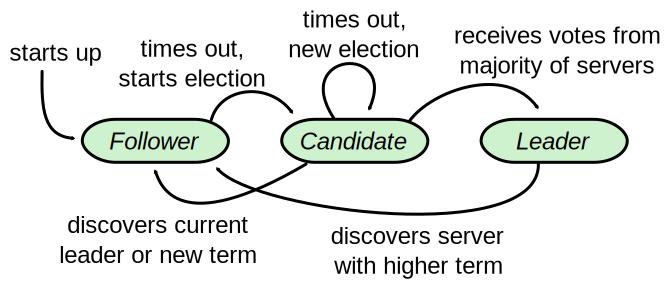
\includegraphics[scale=.50]{basicraft/followercandidateleader}
\vcaption[server states]{
Server states. Followers only respond to
requests from other servers. If a follower receives no communication, 
it becomes a candidate and initiates an election. A candidate
that receives votes from a majority of the full cluster becomes the new
leader. Leaders typically operate until they fail.}
\label{fig:basicraft:followercandidateleader}
\end{figure}

\begin{figure}
\centering
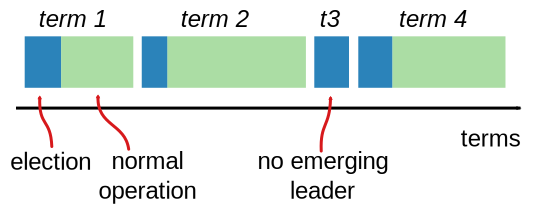
\includegraphics[scale=.50]{basicraft/terms}
\vcaption[terms]{
Time is divided into terms, and each term begins with an election. After
a successful election, a single leader manages the cluster until the end
of the term. Some elections fail, in which case the term ends without
choosing a leader.
The transitions between terms may be observed at different times on
different servers. 
}
\label{fig:basicraft:terms}
\end{figure}

Different servers may observe the transitions between terms
at different times, and in some situations a server may not observe
an election or even entire terms.
Terms act as a logical clock~\cite{Lamport:1978} in \name{},
and they allow
servers to detect obsolete information such as stale leaders.
Each server stores a \emph{current term} number, which increases
monotonically over time. Current terms are exchanged whenever
servers communicate; if one server's current term is smaller than
the other's, then it updates its current term to the larger value.
If a candidate or leader discovers that its term is out of date,
it immediately reverts to follower state.
If a server receives a request with a stale term number, it
rejects the request.

Raft servers communicate using remote procedure calls (RPCs), and the
basic consensus algorithm requires only two types of RPCs between
servers. RequestVote RPCs are initiated by candidates during elections
(Section~\ref{basicraft:leaderelection}), and AppendEntries RPCs are
initiated by leaders to replicate log entries and to provide a form of
heartbeat (Section~\ref{basicraft:logreplication}). Leadership transfer
(Section~\ref{basicraft:leadershiptransfer}) and the mechanisms
described in subsequent chapters introduce additional RPCs beyond the
two in the core consensus algorithm.

We chose to structure communication in Raft as RPCs to simplify
its communication patterns. Each request type has a corresponding response
type, which also serves as the request's acknowledgment. Raft assumes RPC
requests and responses may be lost in the network; it is the requester's
responsibility to retry the RPC if it does not receive a response in a
timely manner. Servers issue RPCs in parallel for best performance, and
Raft does not assume the network preserves ordering between RPCs.

\section{Leader election}
\label{basicraft:leaderelection}

\name{} uses a heartbeat mechanism to trigger leader election.
When servers start up, they begin
as followers. A server remains in follower state as long as it
receives valid RPCs from a leader or candidate. Leaders send periodic
heartbeats (AppendEntries RPCs that carry no log entries) to all
followers in order to maintain their authority. If a follower
receives no communication over a
period of time called the \emph{election timeout}, then
it assumes there is no viable leader and
begins an election to choose a new leader.



To begin an election, a follower increments its current term and
transitions to candidate state. It then votes for itself and issues RequestVote RPCs in
parallel to each of the other servers in the cluster.
A candidate continues in this state until one of three things
happens: (a) it wins the election, (b) another server establishes
itself as leader, or (c) another
election timeout goes by with no winner.
These outcomes are discussed separately in the paragraphs below.

A candidate wins an election if it receives votes from a majority
of the servers in the full cluster for the same term. Each server will
vote for at most one candidate in a given term, on a
first-come-first-served basis (note: Section~\ref{basicraft:safety} adds
an additional restriction on votes). The
majority rule ensures that at most one candidate can win
the election for a particular term (the Election Safety Property
in Figure~\ref{fig:basicraft:properties}).
Once a candidate wins an election, it becomes leader.
It then sends heartbeat messages to
all of the other servers to establish its authority and prevent new elections.

While waiting for votes, a candidate may receive an AppendEntries RPC
from another server claiming to be leader. If the leader's term
(included in its RPC) is at least as large as the candidate's
current term, then the candidate recognizes the leader as legitimate
and returns to follower state.
If the term in the RPC is smaller than the candidate's current term,
then the candidate rejects the RPC and continues in candidate state.

The third possible outcome is that a candidate neither wins nor loses
the election:
if many followers become candidates at the same time, votes could be
split so that no candidate obtains a majority. When this happens,
each candidate will time out and start
a new election by incrementing its term and initiating another round
of RequestVote RPCs. However, without extra measures
split votes could repeat indefinitely.

\name{} uses randomized election timeouts to ensure that split votes
are rare and that they are resolved quickly. To prevent split
votes in the first place, election timeouts are chosen randomly
from a fixed interval (e.g., \SIrange{150}{300}{\milli\second}).
This spreads out the servers
so that in most cases only a single server will time out; it wins the
election and sends heartbeats before any other servers time out.
The same mechanism is used to handle split votes. Each candidate
restarts its randomized election timeout at the start of an election,
and it waits for that timeout to elapse before starting the
next election; this reduces the likelihood of
another split vote in the new election.
Chapter~\ref{leaderelection} shows that this approach
elects a leader rapidly.


Elections are an example of how understandability guided
our choice between design alternatives. Initially we planned to use
a ranking system: each candidate was assigned a unique
rank, which was used to select between competing candidates.
If a candidate discovered another candidate with higher
rank, it would return to follower state so that the
higher ranking candidate could more easily win the next election.
We found that this approach
created subtle issues around availability
(a lower-ranked server might need to time out and become a
candidate again if a higher-ranked server fails, but if it does so too
soon, it can reset progress towards electing a leader).
We made adjustments to the algorithm
several times, but after each adjustment new corner cases appeared.
Eventually we concluded that the randomized retry approach is more
obvious and understandable.

\section{Log replication}
\label{basicraft:logreplication}

Once a leader has been elected, it begins servicing client requests.
Each client request contains a
command to be executed by the replicated state machine.
The leader appends the command to its log as a new entry, then issues
AppendEntries RPCs in parallel to each of the other servers to
replicate the entry.
When the entry has been safely replicated (as described below),
the leader
applies the entry to its state machine and
returns the result of
that execution to the client. If followers crash or run slowly, or
if network packets are lost, the leader retries AppendEntries RPCs
indefinitely (even after it has responded to the client)
until all followers eventually store all log entries.

\begin{figure}
\centering
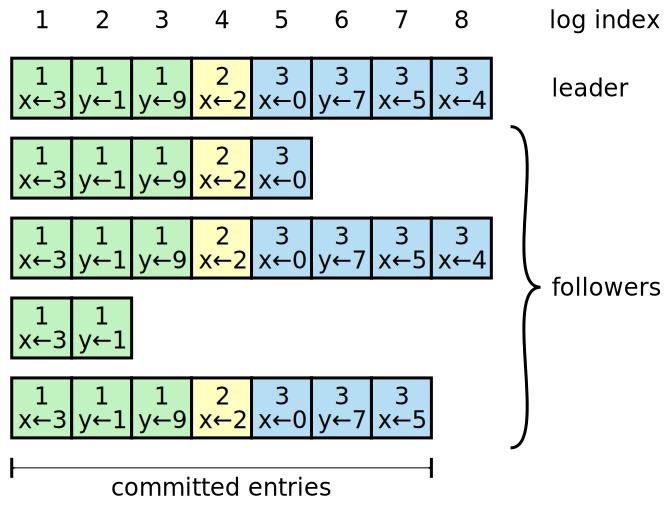
\includegraphics[scale=.50]{basicraft/log2}
\vcaption[log structure]{
Logs are composed of entries, which are numbered sequentially. Each
entry contains the term in which it was created (the number in each
box) and a command for the state machine. An entry is considered
\emph{committed} if it is safe for that entry to be applied to
state machines.}
\label{fig:basicraft:log}
\end{figure}

Logs are organized as shown in Figure~\ref{fig:basicraft:log}.
Each log entry stores a state machine command along with the
term number when the entry was received by the leader.
The term numbers in log entries are used to detect inconsistencies
between logs and to ensure some of the properties in
Figure~\ref{fig:basicraft:properties}. Each log entry
also has an integer index identifying its position in the log.

The leader decides when it is safe to apply a log entry to the
state machines; such an entry is called \emph{committed}.
\name{} guarantees that committed entries are durable
and will eventually be executed by all of the available state machines.
A log entry is committed once the leader that created the
entry has replicated it on a majority of the servers
(e.g., entry 7 in Figure~\ref{fig:basicraft:log}). 
This also commits all preceding entries in the leader's log, including
entries created by previous leaders.
Section~\ref{basicraft:safety} discusses some subtleties when applying
this rule after leader changes, and it also shows
that this definition of commitment is safe.
The leader keeps track of the highest index
it knows to be committed, and it includes
that index in future AppendEntries RPCs (including heartbeats) so
that the other servers eventually find out. Once a follower
learns that a log entry is committed, it applies the entry
to its local state machine (in log order).

We designed the \name{} log mechanism to maintain a high level
of coherency between the logs on different servers. Not only does this
simplify the system's behavior and make it more predictable,
but it is an important component of ensuring safety.
\name{} maintains
the following properties,
which together constitute the Log Matching Property in
Figure~\ref{fig:basicraft:properties}:
\begin{compactitem}
\item If two entries in different logs have the same index and term,
then they store the same command.
\item If two entries in different logs have the same index and term,
then the logs are identical in all preceding entries.
\end{compactitem}

The first property follows from the fact
that a leader creates at most one entry with a given log index
in a given term, and log entries never change their position in
the log.
The second property is guaranteed by a consistency check
performed by AppendEntries. When sending an AppendEntries RPC,
the leader
includes the index and term of the entry in its log that immediately
precedes the new entries.
If the follower does not find an entry in its log with the same
index and term, then it refuses the new entries.
The consistency check acts as an induction step: the
initial empty state of the logs satisfies the
Log Matching Property,
and the consistency check preserves the
Log Matching Property whenever logs are
extended. As a result, whenever AppendEntries returns successfully,
the leader knows that the follower's log is identical to its own log
up through the new entries.

During normal operation, the logs of the leader and followers stay
consistent, so the AppendEntries consistency check never fails.
However, leader crashes can leave the logs inconsistent (the old
leader may not have fully replicated all of the entries in its log).
These inconsistencies can compound over a series of leader and
follower crashes. Figure~\ref{fig:basicraft:diverge} illustrates
the ways in which followers' logs may differ from that of a
new leader. A follower may be missing entries that are present
on the leader, it may have extra entries that are
not present on the leader, or both.
Missing and extraneous entries in a log may span
multiple terms.

In \name{}, the leader handles
inconsistencies by forcing the followers' logs to duplicate its own.
This means that conflicting entries in follower logs will be overwritten
with entries from the leader's log.
Section~\ref{basicraft:safety} will 
show that this is safe when coupled with a restriction on elections.

\begin{figure}
\centering
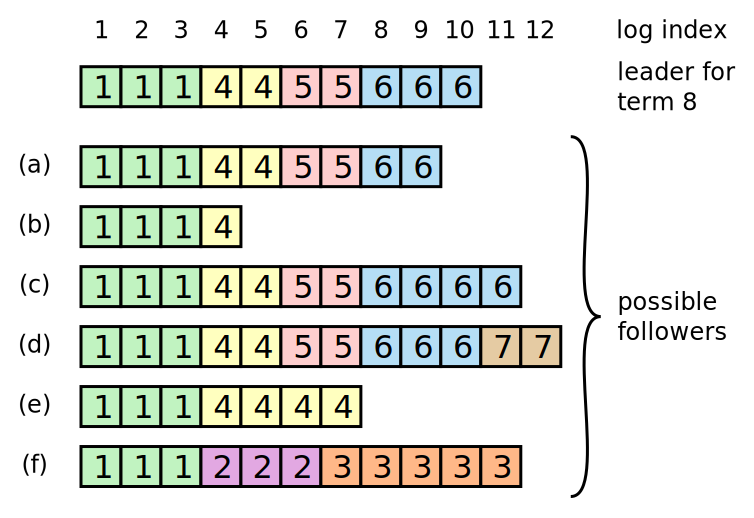
\includegraphics[scale=.50]{basicraft/diverge2}
\vcaption[log inconsistencies]{
When the leader at the top comes to power, it is possible that
any of scenarios (a--f) could occur in follower logs. Each box
represents one log entry; the number in the box is
its term. A follower may be missing entries (a--b), may have extra
uncommitted entries (c--d), or both (e--f). For example, scenario (f)
could occur if that server was the leader for term~2, added several entries
to its log, then crashed before committing any of them; it
restarted quickly, became leader for term 3, and added a few more
entries to its log; before any of the entries in either term 2 or term 3
were committed, the server crashed again and remained down for several terms.
}
\label{fig:basicraft:diverge}
\end{figure}

To bring a follower's log into consistency with its own,
the leader must find the latest log entry where the two logs agree,
delete any entries in the follower's log after that point,
and send the follower all of the leader's entries after that point.
All of these actions happen in response to the consistency check performed
by AppendEntries RPCs.
The leader maintains a \emph{nextIndex} for each follower, which
is the index of the next log entry the leader will send to that
follower. When a leader first comes to power, it initializes all nextIndex values
to the index just after the last one in its log (11 in
Figure~\ref{fig:basicraft:diverge}).
If a follower's log is inconsistent with the leader's, the AppendEntries
consistency check will fail in the next AppendEntries RPC.
After a rejection, the leader decrements the follower's nextIndex
and retries the AppendEntries
RPC. Eventually the nextIndex will reach a point where the leader and
follower logs match.
When this happens, AppendEntries will
succeed, which removes any conflicting entries in the follower's
log and appends
entries from the leader's log (if any). Once AppendEntries succeeds, the
follower's log is consistent with the leader's, and it will remain that way
for the rest of the term.

Until the leader has discovered where it and the follower's logs match,
the leader can send AppendEntries with no entries (like heartbeats) to
save bandwidth. Then, once the matchIndex immediately precedes the nextIndex,
the leader should begin to send the actual entries.

If desired, the protocol can be optimized to reduce the number of rejected
AppendEntries RPCs.  For example, when rejecting an AppendEntries request, the
follower can include the term of the conflicting entry
and the first index it stores for that term. With this
information, the leader can decrement nextIndex to bypass all of the conflicting
entries in that term; one AppendEntries RPC will be required for each term
with conflicting entries, rather than one RPC per entry.
Alternatively, the leader can use a binary search approach to find
the first entry where the follower's log differs from its own; this has
better worst-case behavior.
In practice, we
doubt these optimizations are necessary, since failures happen infrequently and
it is unlikely that there will be many inconsistent entries.

With this mechanism, a leader does not need to take any special actions
to restore log consistency when it comes to power. It just begins normal
operation, and the logs automatically converge in response to
failures of the AppendEntries consistency check.
A leader never overwrites or deletes entries in its own log (the Leader
Append-Only Property in Figure~\ref{fig:basicraft:properties}).

This log replication mechanism exhibits the desirable consensus properties
described in Section~\ref{motivation:problem}: \name{} can accept, replicate, and
apply new log entries as long as a majority of the servers are up;
in the normal case a new entry can be replicated with a single round
of RPCs to a majority of the cluster;
and a single slow follower will not impact performance.
The log replication algorithm is also practical to implement, since
AppendEntries requests are manageable in size (leaders never need to
send more than one entry in a single AppendEntries request to make
progress). Some other consensus algorithms are described as
sending entire logs over the network; this places a burden on the
implementer to develop optimizations required for a practical
implementation.

\section{Safety}
\label{basicraft:safety}

The previous sections described how \name{} elects leaders and
replicates log entries. However, the mechanisms described so far are not
quite sufficient to ensure that each state machine executes exactly the
same commands in the same order. For example, a follower might be
unavailable while the leader commits several log entries, then it
could be elected leader and overwrite these entries with new ones;
as a result, different state machines might execute different command
sequences.

This section completes the \name{} algorithm by adding a restriction
on which servers may be elected leader. The restriction ensures that the leader
for any given term contains all of the entries committed in previous
terms (the Leader Completeness Property from Figure~\ref{fig:basicraft:properties}).
Given the election restriction, we then make the rules for commitment
more precise. Finally, we present a proof sketch for the Leader
Completeness Property and show how it leads to correct
behavior of the replicated state machine.

\subsection{Election restriction}

In any leader-based consensus algorithm, the leader must eventually store
all of the committed log entries. In some consensus algorithms, such
as Viewstamped Replication~\cite{Liskov:2012},
a leader can be elected even if it doesn't initially contain all of the
committed entries. These algorithms contain additional mechanisms to identify
the missing entries and transmit them to the new leader, either during the
election process or shortly afterwards. Unfortunately, this results in
considerable additional mechanism and complexity. \name{} uses a simpler
approach where it guarantees that all the committed entries from previous
terms are present on each new leader from the moment of its election,
without the need to transfer those entries to the leader. This means
that log entries only flow in one direction, from leaders
to followers, and leaders never overwrite existing entries in their logs.

\begin{figure}
\centering
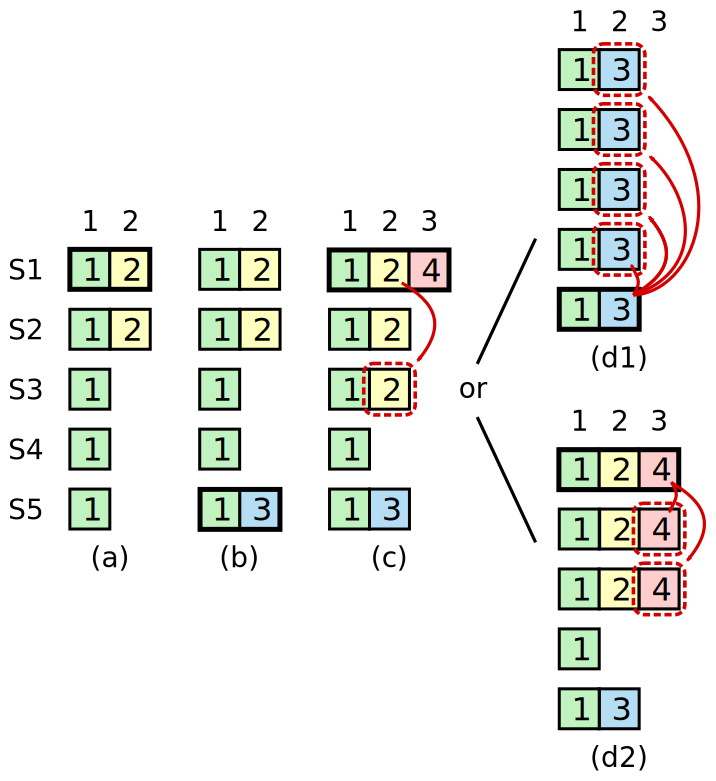
\includegraphics[scale=.50]{basicraft/oldTermCommit}
\vcaption[commitment rule]{
A time sequence showing why a leader cannot determine commitment
using log entries from older terms. In (a) S1 is leader and
partially replicates the log entry at index 2. In (b) S1 crashes;
S5 is elected leader for term 3 with votes from S3,
S4, and itself, and accepts a different entry at log index 2.
In (c) S5 crashes; S1 restarts, is elected leader, and continues
replication. At this point, the log entry from term 2 has been replicated
on a majority of the servers, but it is not committed. If S1 crashes
as in (d1), S5 could be elected leader (with votes from S2, S3,
and S4) and overwrite the entry with its own entry from term 3.
However, if S1 replicates an entry from its current term on a
majority of the servers before crashing, as in (d2), then this entry is
committed (S5 cannot win an election). At this point all preceding
entries in the log are committed as well.
}
\label{fig:basicraft:oldTermCommit}
\end{figure}

\name{} uses the voting process to prevent a candidate from winning
an election unless its log contains all committed entries. A candidate
must contact a majority of the cluster in order to be elected, which
means that every committed entry must be present in at least one of
those servers. If the candidate's log is at least as up-to-date as
any other log in that majority (where ``up-to-date'' is defined
precisely below), then it will hold all the committed entries.
The RequestVote RPC implements this restriction: the RPC includes
information about the candidate's log, and the voter denies
its vote if its own log is more up-to-date than that of the candidate.

\name{} determines which of two logs is more up-to-date by comparing
the index and term of the last entries in the logs. If
the logs have last entries with different terms, then the log with
the later term is more up-to-date. If the logs end with the same term,
then whichever log is longer is more up-to-date.

\subsection{Committing entries from previous terms}
As described in Section~\ref{basicraft:logreplication}, a leader knows
that an entry from its current term is committed once that entry
is stored on a majority of the servers. If a leader crashes
before committing an entry, future leaders will attempt to finish
replicating the entry. However, a leader cannot
immediately conclude that an entry from a previous term is
committed once it is stored on a majority of servers.
Figure~\ref{fig:basicraft:oldTermCommit}
illustrates a situation where an old log entry is stored on a
majority of servers, yet can still be overwritten by a future leader.

To eliminate problems like the one in
Figure~\ref{fig:basicraft:oldTermCommit}, Raft never commits log entries
from previous terms by counting replicas. Only log entries
from the leader's current term are committed by counting replicas;
once an entry from the current term has been committed in this way,
then all prior entries are committed
indirectly because of the Log Matching Property. There are some
situations where a leader could safely conclude
that an older log entry is committed (for example, if that entry is stored
on every server), but Raft takes a more conservative approach
for simplicity.

Raft incurs this extra complexity in the commitment rules because
log entries retain their original term numbers when a leader
replicates entries from previous terms. In other consensus algorithms,
if a new leader re-replicates entries from prior ``terms'',
it must do so with its new ``term number''. Raft's
approach makes it easier to reason about log entries, since they
maintain the same term number over time and across logs. In
addition, new leaders in Raft
send fewer log entries from previous terms than in other algorithms,
since other algorithms must send redundant log entries to renumber them
before they can be committed; however, this may not be very
important in practice, since leader changes should be rare.

\subsection{Safety argument}
\label{basicraft:safety:argument}

\newcommand\leaderT{$\textrm{leader}_\textrm{T}$}
\newcommand\leaderU{$\textrm{leader}_\textrm{U}$}

Given the complete Raft algorithm, we can now argue
more precisely that the Leader Completeness Property holds
(this argument is based on the safety proof; see
Chapter~\ref{correctness}).
We assume that the Leader Completeness Property
does not hold, then we prove a contradiction.
Suppose the leader for term T (\leaderT{}) commits a log entry from
its term, but that log entry is not stored by the leader of some
future term. Consider the smallest term U $>$ T whose leader (\leaderU{})
does not store the entry.

\begin{figure}
\centering
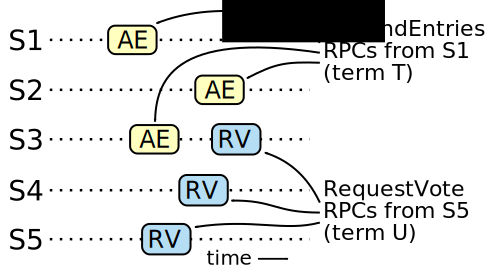
\includegraphics[scale=.50]{basicraft/safety2}
\vcaption[existence of voter in safety argument]{
If S1 (leader for term T) commits a new log entry from its term,
and S5 is elected leader for a later term U, then
there must be at least one server (S3) that accepted the log entry
and also voted for S5.
}
\label{fig:basicraft:safety2}
\end{figure}


\begin{enumerate}

\item The committed entry must have been absent from \leaderU{}'s log
at the time of its election (leaders never delete or overwrite entries).

\item \leaderT{} replicated the entry on a majority of the
cluster, and \leaderU{} received votes from a majority of
the cluster. Thus, at least one server (``the voter'') both accepted
the entry from \leaderT{} and voted for \leaderU{}, as shown
in Figure~\ref{fig:basicraft:safety2}. The voter is key to reaching a
contradiction.

\item  The voter must have accepted the committed entry from \leaderT{}
\emph{before} voting for \leaderU{}; otherwise it would have rejected
the AppendEntries request from \leaderT{} (its current term would
have been higher than T).

\item The voter still stored the entry when it voted for
\leaderU{}, since every intervening leader contained
the entry (by assumption), leaders never remove entries, and followers
only remove entries if they conflict with the leader.

\item The voter granted its vote to \leaderU{}, so \leaderU{}'s log must
have been as up-to-date as the voter's. This leads to one of two
contradictions.

\item First, if the voter and \leaderU{} shared the same last log term,
then \leaderU{}'s log must have been at least as long as the voter's,
so its log contained every entry in the voter's log. This is a contradiction,
since the voter contained the committed entry and \leaderU{} was assumed
not to.

\item Otherwise, \leaderU{}'s last log term must have been larger than
the voter's.
Moreover, it was larger than T, since the voter's last log term was at
least T (it contains the committed entry from term T). The earlier
leader that created \leaderU{}'s last log entry must have contained
the committed entry in its log (by assumption).
Then, by the Log Matching Property, \leaderU{}'s log must also contain
the committed entry, which is a contradiction.

\item This completes the contradiction. Thus, the leaders of all terms
greater than T must contain all entries from term T that are committed
in term T.

\item The Log Matching Property guarantees that future leaders
will also contain entries that are committed indirectly, such as
index 2 in Figure~\ref{fig:basicraft:oldTermCommit}(d2).

\end{enumerate}

Given the Leader Completeness Property, we can prove the State Machine
Safety Property from Figure~\ref{fig:basicraft:properties}, which states that
if a server has applied a log entry at a given index to its state
machine, no other server will ever apply a different log entry for the
same index.
At the time a server applies a log entry to its state machine, its log
must be identical to the leader's log up through that entry, and the
entry must be committed. Now consider the lowest term
in which any server applies a given log index; the Leader Completeness Property
guarantees that the leaders for all higher terms will store that same log
entry, so servers that apply the index in later terms will apply the same
value. Thus, the State Machine Safety Property holds.

Finally, \name{} requires servers to apply entries in log index order.
Combined with the State Machine Safety Property, this means that all
servers will apply exactly the same set of log entries to their state
machines, in the same order.

\section{Follower and candidate crashes}
Until this point we have focused on leader failures.
Follower and candidate crashes are much simpler to handle than leader
crashes, and they are both handled in the same way.
If a follower or candidate crashes (or the network link between it and
the leader fails), then future RequestVote and AppendEntries
RPCs sent to it will fail. Raft handles these failures by
retrying indefinitely;
if the crashed server restarts, then the RPC will complete
successfully.
If a server crashes after
completing an RPC but before responding, then it will receive the same
RPC again after it restarts. Raft RPCs have the same effect if repeated,
so this causes no harm. For example, if a follower receives an
AppendEntries request that includes log entries already present in
its log, it ignores those entries in the new request.

\section{Persisted state and server restarts}

Raft servers must persist enough information to stable storage to
survive server restarts safely. In particular, each server persists its
current term and vote; this is necessary to prevent the server from
voting twice in the same term or replacing log entries from a newer
leader with those from a deposed leader. Each server also persists new
log entries before they are counted towards the entries' commitment;
this prevents committed entries from being lost or ``uncommitted'' when
servers restart.

Other state variables are safe to lose on a restart, as they can all be
recreated.
The most interesting example is the commit index, which can safely be
reinitialized to zero on a restart. Even if every server restarts at the
same time, the commit index will only temporarily lag behind its true
value. Once a leader is elected and is able to commit a new entry, its
commit index will advance, and it will quickly propagate this commit
index to its followers.

The state machine can either be volatile or persistent. A volatile state
machine must be recovered after restarts by reapplying log entries
(after applying the latest snapshot; see Chapter~\ref{compaction}). A
persistent state machine, however, has already applied most entries
after a restart; to avoid reapplying them, its \emph{last applied} index
must also be persistent.

If a server loses any of its persistent state, it cannot safely rejoin
the cluster with its prior identity. Such a server can
usually be added back into the cluster with a new identity by invoking a
cluster membership change (see Chapter~\ref{membership}). If a majority
of the cluster loses its persistent state, however, log entries may be
lost and progress on cluster membership changes will not be possible; to
proceed, a system administrator would need to admit the possibility of
data loss.

\section{Timing and availability}
\label{basicraft:timing}

One of our requirements for \name{} is that safety must not depend
on timing: the system must not produce incorrect results just because
some event happens more quickly or slowly than expected. However,
availability (the ability of the system to respond to clients in a
timely manner) must
inevitably depend on timing. For example, if message exchanges take
longer than the typical time between server crashes, candidates will
not stay up long enough to win an election; without a steady leader,
\name{} cannot make progress.

Leader election is the aspect of \name{} where timing is most
critical. \name{} will be able to elect and maintain a steady
leader when the system satisfies the following
\emph{timing requirement}:
\begin{equation*}
\mathit{broadcastTime} \ll \mathit{electionTimeout} \ll \mathit{MTBF}
\end{equation*}
In this inequality \emph{broadcastTime} is the average time it takes a
server to send RPCs in parallel to every server in the cluster and receive
their responses; \emph{electionTimeout} is the election timeout described
in Section~\ref{basicraft:leaderelection}; and \emph{MTBF} is the
mean (average) time between failures for a
single server. The broadcast time should be an order of magnitude less than the
election timeout so that leaders can reliably send the heartbeat messages
required to keep followers from starting elections; given the randomized
approach used for election timeouts, this inequality also makes split votes
unlikely. 
The election timeout should be a few orders of magnitude less than MTBF
so that the system
makes steady progress. When the leader crashes, the system will be
unavailable for roughly the election timeout; we would like this to
represent only a small fraction of overall time.

The broadcast time and MTBF are properties of the underlying system, while
the election timeout is something we must choose. \name{}'s RPCs typically
require the recipient to persist information to stable storage, so the
broadcast time may range from \SIrange{0.5}{20}{\milli\second},
depending on storage
technology. As a result, the election
timeout is likely to be somewhere between
\SIrange{10}{500}{\milli\second}.
Typical server MTBFs are several months or more, which
easily satisfies the timing requirement.
Chapter~\ref{leaderelection} explores how to set the election timeout
and its impact on availability and leader election performance in more
detail.

\section{Leadership transfer extension}
\label{basicraft:leadershiptransfer}

This section describes an optional extension to Raft that allows one
server to transfer its leadership to another. Leadership transfer could
be useful in two types of situations:
%
\begin{enumerate}
%
\item Sometimes the leader must step down. For example, it may
need to reboot for maintenance, or it may be removed from the cluster
(see Chapter~\ref{membership}). When it steps down, the cluster will be
idle for an election timeout until another server times out and wins an
election. This brief unavailability can be avoided by having the leader
transfer its leadership to another server before it steps down.
%
\item In some cases, one or more servers may be more suitable to lead
the cluster than others. For example, a server with high load would not
make a good leader, or in a WAN deployment, servers in a primary
datacenter may be preferred in order to minimize the latency between
clients and the leader. Other consensus algorithms may be able
to accommodate these preferences during leader election, but Raft needs
a server with a sufficiently up-to-date log to become leader, which
might not be the most preferred one. Instead, a leader in Raft
can periodically check to see whether one of its available followers
would be more suitable, and if so, transfer its leadership to that
server. (If only human leaders were so graceful.)
%
\end{enumerate}

To transfer leadership in Raft, the prior leader sends its log entries to
the target server, then the target server runs an election without
waiting for an election timeout to elapse.
The prior leader thus ensures that the target server has all committed
entries at the start of its term, and, as in normal elections, the
majority voting guarantees the safety properties (such as the Leader
Completeness Property) are maintained. The following steps describe the
process in more detail:
%
\begin{enumerate}
%
\item The prior leader stops accepting new client requests.
%
\item The prior leader fully updates the target server's log to match
its own, using the normal log replication mechanism described in
Section~\ref{basicraft:logreplication}.
%
\item The prior leader sends a \emph{TimeoutNow} request to the target
server. This request has the same effect as the target server's election
timer firing: the target server starts a new election (incrementing its
term and becoming a candidate).
%
\end{enumerate}
%
Once the target server receives the TimeoutNow request, it is highly
likely to start an election before any other server and become leader in
the next term. Its next message to the prior leader will include its new
term number, causing the prior leader to step down. At this point,
leadership transfer is complete.

It is also possible for the target server to fail; in this case, the
cluster must resume client operations. If leadership transfer does not
complete after about an election timeout, the prior leader aborts the
transfer and resumes accepting client requests. If the prior leader was
mistaken and the target server is actually operational, then at worst
this mistake will result in an extra election, after which client
operations will be restored.

This approach preserves safety by operating within the normal
transitions of a Raft cluster. For example, Raft already guarantees
safety even when clocks run at arbitrary speeds; when the target server
receives a TimeoutNow request, it is equivalent to the target server's
clock jumping forwards quickly, which is safe. However, we have not currently
implemented or evaluated this leadership transfer approach.

\section{Conclusion}
\label{basicraft:conclusion}

This chapter addressed all the core problems for a consensus-based
system. Raft goes beyond reaching consensus on a single value, as in
single-decree Paxos; it achieves consensus on a growing log of commands,
which is needed to build a replicated state machine. It also
includes disseminates information once agreement has been reached, so
that other servers learn the log entries that have been committed. Raft
achieves consensus in a practical and efficient way by electing a
cluster leader to unilaterally make decisions and transmitting only the
necessary log entries when a new leader comes to power. We have
implemented the ideas of Raft in LogCabin, a replicated state machine
(described in Chapter~\ref{performance}).

Raft uses only a small amount of mechanism to address the full consensus
problem. For example, it uses only two RPCs (RequestVote and
AppendEntries). Perhaps surprisingly, creating a compact
algorithm/implementation was not an explicit goal for Raft. Rather, it
is a result of our design for understandability, where every bit of
mechanism must be fully motivated and explained. We found that redundant
or meandering mechanism is hard to motivate, so it naturally gets purged
in the design process.

Unless we felt confident that a particular problem would affect a large
fraction of Raft deployments, we did not address it in Raft. As a
result, parts of Raft may appear na\"ive. For example, servers in Raft
detect a split vote by waiting for an election timeout; in principle,
they could often detect and even resolve split votes sooner by counting
the votes granted to any candidate. We chose not to develop this
optimization for Raft, since it adds complexity but probably brings no
practical benefit: split votes are rare in a well-configured deployment.
Other parts of Raft may appear overly conservative. For example, a
leader only directly commits an entry from its current term, even though
in some special cases it could safely commit entries from prior terms.
Applying a more complex commitment rule would harm understandability and
would not have a significant effect on performance; commitment is only
delayed briefly with the current rule. In discussing Raft with others,
we found that many people cannot help but think of such optimizations
and propose them, but when the goal is understandability, premature
optimizations should be left out.

Inevitably, this chapter might have left out some features or
optimizations that turn out to be useful in practice. As implementers
gain more experience with Raft, they will learn when and why certain
additional features may be useful, and they may need to implement these
for some practical deployments. Throughout the chapter, we sketched a
few optional extensions that we currently think are unnecessary but that
may help guide implementers should the need arise. By focusing on
understandability, we hope to have provided a solid foundation for
implementers to adjust Raft according to their experiences. Since Raft
works in our testing environment, we expect these to be straightforward
extensions rather than fundamental changes.


\chapter{Cluster membership changes}
\label{membership}

Up until now we have assumed that the cluster \emph{configuration}
(the set of servers participating in the consensus algorithm) is fixed.
In practice, it will occasionally be necessary to change the
configuration, for example to replace servers when they fail or to
change the degree of replication. This could be done
manually, using one of two approaches:
\begin{itemize}
\item Configuration changes could be done by taking the entire cluster
off-line, updating configuration files, and then restarting the cluster.
However, this would leave the cluster unavailable during the changeover.
\item Alternatively, a new server could replace a cluster member by
acquiring its network address. However, the administrator must guarantee
that the replaced server will never come back up, or else the system
would lose its safety properties (for example, there would be an extra
vote).
\end{itemize}
Both of these approaches to membership changes have significant downsides,
and if there are any manual steps, they risk operator error.

\begin{figure}
\centering
\includegraphics[scale=0.95]{membership/cheatsheet2}
\vcaption[RPCs to change cluster membership]{
RPCs used to change cluster membership. The
AddServer RPC is used to add a new server to the current configuration,
and the RemoveServer RPC is used to remove a server from the current
configuration.
Section numbers such as \S\ref{membership:safety} indicate where
particular features are discussed.
Section~\ref{membership:system} discusses ways to use
these RPCs in a complete system.
}
\label{fig:membership:cheatsheet2}
\end{figure}


In order to avoid these issues, we decided to automate configuration
changes and incorporate them into the \name{} consensus algorithm. Raft
allows the cluster to continue operating normally during changes, and
membership changes can be implemented with only a few extensions to the
basic consensus algorithm. Figure~\ref{fig:membership:cheatsheet2}
summarizes the RPCs used to change cluster membership, whose elements
are described in the remainder of this chapter.


\section{Safety}
\label{membership:safety}

Preserving safety is the first challenge for configuration changes.
For the mechanism to be safe,
there must be no point during the transition where it is possible for
two leaders to be elected for the same term. If a single configuration
change adds or removes many servers, switching the cluster directly from
the old configuration to the new configuration can be unsafe;
it isn't possible to atomically switch all of the servers at once, so 
the cluster can potentially split into two independent majorities
during the transition (see
Figure~\ref{fig:membership:reconfigurationdifficulty}).

\begin{figure}
\centering
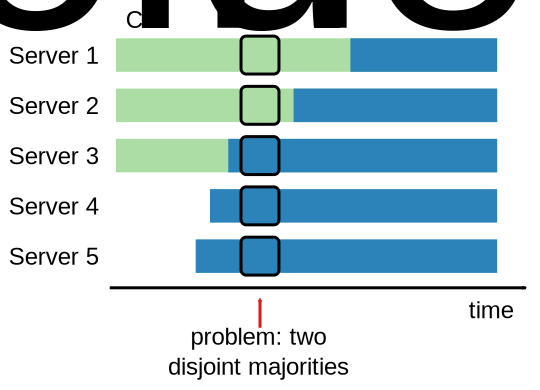
\includegraphics[scale=.50]{membership/reconfigurationdifficulty}
\vcaption[safety challenge]{
Switching directly from one configuration to another can be
unsafe because different servers will switch at different times.
In this example, the cluster grows from three servers to five.
Unfortunately, there is a point in time where two different leaders
can be elected for the same term,
one with a majority of the old
configuration (\cold{}) and another with a majority of the new
configuration (\cnew{}).
}
\label{fig:membership:reconfigurationdifficulty}
\end{figure}

\begin{figure}
\centering

\begin{subfigure}{.45\textwidth}
\centering
\includegraphics[scale=0.50]{membership/special4to5}
\caption{
Adding one server to a 4-server cluster.
}
\end{subfigure}
~
\begin{subfigure}{.45\textwidth}
\centering
\includegraphics[scale=0.50]{membership/special3to4}
\caption{
Adding one server to a 3-server cluster.
}
\end{subfigure}

\vspace{3ex}

\begin{subfigure}{.45\textwidth}
\centering
\includegraphics[scale=0.50]{membership/special5to4}
\caption{
Removing one server from a 5-server cluster.
}
\end{subfigure}
~
\begin{subfigure}{.45\textwidth}
\centering
\includegraphics[scale=0.50]{membership/special4to3}
\caption{
Removing one server from a 4-server cluster.
}
\end{subfigure}

\vcaption[adding/removing one server maintains overlap]{
The addition and removal of a single server from an even- and an
odd-sized cluster.
In each figure,
the blue rectangle shows a majority of the old cluster, and the red
rectangle shows a majority of the new cluster.
In every single-server membership change, an overlap between any majority
of the old cluster and any majority of the new cluster is preserved,
as needed for safety. For example in (b), a majority of the old cluster
must include two of the left three servers, and a majority of the new
cluster must include three of the servers in the new cluster, of which
at least two must come from the old cluster.
}
\label{fig:membership:special}
\end{figure}

Most membership change algorithms introduce additional mechanism to deal
with such problems. This is what we did for Raft initially, but we later
discovered a simpler approach, which is to disallow membership changes
that could result in disjoint majorities. Thus, Raft restricts the types
of changes that are allowed: only one server can be added or removed
from the cluster at a time. More complex changes in membership are
implemented as a series of single-server changes. Most of this chapter
describes the single-server approach, which is easier to understand than
our original approach. For completeness,
Section~\ref{membership:arbitrary} describes the original approach,
which incurs additional complexity to handle arbitrary configuration
changes. We implemented the more complex approach in LogCabin prior to
discovering the simpler single-server change approach; it still uses the
more complex approach at the time of this writing.

When adding a single server to a cluster or removing a single server
from a cluster, any majority of the old cluster overlaps with any
majority of the new cluster; see Figure~\ref{fig:membership:special}.
This overlap prevents the cluster from splitting into two independent
majorities; in terms of the safety argument of
Section~\ref{basicraft:safety:argument}, it guarantees the existence of
``the voter''. Thus, when adding or removing just a single server, it is
safe to switch directly to the new configuration. Raft exploits this
property to change cluster membership safely using little additional
mechanism.

Cluster configurations are stored and communicated using special entries
in the replicated log.
This leverages the existing mechanisms in Raft to
replicate and persist configuration information.
It also allows the cluster to continue to service
client requests while configuration changes are in progress,
by imposing ordering between
configuration changes and client requests (while allowing both to be
replicated concurrently in a pipeline and/or in batches).

When the leader receives a request to add or remove a server from its
current configuration (\cold{}), it appends the new configuration
(\cnew{}) as an entry in its log and replicates that entry using the
normal Raft mechanism. The new configuration takes effect on each server
as soon as it is added to that server's log: the \cnew{} entry is
replicated to the \cnew{} servers, and a majority of the new
configuration is used to determine the \cnew{} entry's commitment. This
means that servers do not wait for configuration entries to be
committed, and each server always uses the latest configuration found in
its log.

The configuration change is complete once the \cnew{} entry is
committed. At this point, the leader knows that a majority of the
\cnew{} servers have adopted \cnew{}. It also knows that any servers
that have not moved to \cnew{} can no longer form a majority of the
cluster, and servers without \cnew{} cannot be elected leader.
Commitment of \cnew{} allows three things to continue:
%
\begin{enumerate}
%
\item The leader can acknowledge the successful completion of the
configuration change.
%
\item If the configuration change removed a server, that server can be
shut down.
%
\item Further configuration changes can be started. Before this point,
overlapped configuration changes could degrade to unsafe situations
like the one in Figure~\ref{fig:membership:reconfigurationdifficulty}.
%
\end{enumerate}

As stated above, servers always use the latest configuration in their
logs, regardless of whether that configuration entry has been committed.
This allows leaders to easily avoid overlapping configuration changes
(the third item above), by not beginning a new change until the previous
change's entry has committed. It is only safe to start another membership
change once a majority of the old cluster has moved to operating under
the rules of \cnew{}. If servers adopted \cnew{} only when they
learned that \cnew{} was committed, Raft leaders would have a difficult
time knowing when a majority of the old cluster had adopted it. They
would need to track which servers know of the entry's commitment, and
the servers would need to persist their commit index to disk; neither of
these mechanisms is required in Raft. Instead, each server
adopts \cnew{} as soon as that entry exists in its log, and the leader
knows it's safe to allow further configuration changes as soon as the
\cnew{} entry has been committed. Unfortunately, this decision does
imply that a log entry for a configuration change can be removed (if
leadership changes); in this case, a server must be prepared to fall
back to the previous configuration in its log.

In Raft, it is the caller's configuration that is used in reaching
consensus, both for voting and for log replication:
%
\begin{itemize}
%
\item A server accepts AppendEntries requests from a leader that
is not part of the server's latest configuration. Otherwise, a new server
could never be added to the cluster (it would never accept any log entries
preceding the configuration entry that adds the server).
%
\item A server also grants its vote to a candidate that is not
part of the server's latest configuration (if the candidate has a
sufficiently up-to-date log and a current term). This vote may
occasionally be needed to keep the cluster available. For example,
consider adding a fourth server to a three-server cluster. If one server
were to fail, the new server's vote would be needed to form a majority
and elect a leader.
%
\end{itemize}
%
Thus, servers process incoming RPC requests without consulting their
current configurations.


\section{Availability}
\label{membership:availability}

Cluster membership changes introduce several issues in preserving the
cluster's availability.
%
Section~\ref{membership:availability:catchup} discusses catching up new
servers before they're added to the cluster, so that they do not stall
commitment of new log entries;
%
Section~\ref{membership:availability:removing} addresses how to phase
out an existing leader if it is removed from the cluster; and
%
Section~\ref{membership:availability:disruptive} describes how to
prevent removed servers from disrupting the leader of the new cluster.
%
Finally, Section~\ref{membership:availability:argument} closes with an
argument for why the resulting membership change algorithm is sufficient
to preserve availability during any membership change.


\subsection{Catching up new servers}
\label{membership:availability:catchup}

\begin{figure}
\centering

\begin{subfigure}{.45\textwidth}
\centering
\includegraphics[scale=1]{membership/catchupone}
\caption{
Failure of S3 while adding S4.
}
\label{fig:membership:catchupone}
\end{subfigure}
~
\begin{subfigure}{.45\textwidth}
\centering
\includegraphics[scale=1]{membership/catchupmany}
\caption{
Adding S3--S6 in quick succession.
}
\label{fig:membership:catchupmany}
\end{subfigure}

\vcaption[how adding servers can put availability at risk]{
Examples of how adding servers with empty logs can put availability at
risk. The figures show the servers' logs in two different clusters. Each
cluster starts out with three servers, S1--S3.
%
In~\subref{fig:membership:catchupone}, S4 is added, then S3 fails. The
cluster should be able to operate normally after one failure, but it
loses availability: it needs three of the four servers to commit a new
entry, but S3 has failed and S4's log is too far behind to append new
entries.
%
In~\subref{fig:membership:catchupmany}, S4--S6 are added in quick
succession. Committing the configuration entry that adds S6 (the third
new server) requires four servers' logs to store that entry, but S4--S6
have logs that are far behind.
%
Neither cluster will be available until the new servers' logs are caught
up.
}
\end{figure}

When a server is added to the cluster, it typically will not store any
log entries. If it is added to the cluster in this state, its log could
take quite a while to catch up to the leader's, and during this time,
the cluster is more vulnerable to unavailability. For
example, a three-server cluster can normally tolerate one failure with
no loss in availability. However, if a fourth server with an empty log
is added to the same cluster and one of the original three servers
fails, the cluster will be temporarily unable to commit new entries (see
Figure~\ref{fig:membership:catchupone}). Another availability issue
can occur if many new servers are added to a cluster in
quick succession, where the new servers are needed to form a majority of
the cluster (see Figure~\ref{fig:membership:catchupmany}). In both
cases, until the new servers' logs were caught up to the leader's, the
clusters would be unavailable.

In order to avoid availability gaps, Raft introduces an additional phase
before the configuration change, in which a new server joins the cluster
as a non-voting member. The leader replicates log entries to it, but it
is not yet counted towards majorities for voting or commitment purposes.
Once the new server has caught up with the rest of the cluster, the
reconfiguration can proceed as described above. (The mechanism to
support non-voting servers can also be useful in other contexts; for
example, it can be used to replicate the state to a large number of
servers, which can serve read-only requests with relaxed consistency.)

The leader needs to determine when a new server is sufficiently caught
up to continue with the configuration change. This requires some care to
preserve availability: if the server is added too soon, the cluster's
availability may be at risk, as described above. Our goal was to keep
any temporary unavailability below an election timeout, since clients
must already be able to tolerate occasional unavailability periods of
that magnitude (in case of leader failures). Moreover, if possible, we
wanted to minimize unavailability further by bringing the new server's
log even closer to the leader's.

The leader should also abort the change if the new server is unavailable
or is so slow that it will never catch up. This check is important:
Lamport's ancient Paxon government broke down because they did not
include it. They accidentally changed the membership to consist of only
drowned sailors and could make no more progress~\cite{Lamport:1998}.
Attempting to add a server that is unavailable or slow is often a
mistake. In fact, our very first configuration change request
included a typo in a network port number; the system correctly aborted
the change and returned an error.

\begin{figure}
\centering

\begin{subfigure}{.43\textwidth}
\centering
\includegraphics[scale=0.50]{membership/catchupstart}
\caption{
Start of round 2.
}
\end{subfigure}
~
\begin{subfigure}{.48\textwidth}
\centering
\includegraphics[scale=0.50]{membership/catchupend}
\caption{
End of round 2.
}
\end{subfigure}

\vcaption[rounds in server catchup algorithm]{
To catch up a new server, the replication of entries to the new server
is split into rounds. Each round completes once the new server has all
of the entries that the leader had in its log at the start of the round.
By then, however, the leader may have received new entries; these are
replicated in the next round.
}
\label{fig:membership:catchup}
\end{figure}

We suggest the following algorithm to determine when a new server is
sufficiently caught up to add to the cluster. The replication of entries
to the new server is split into rounds, as shown in
Figure~\ref{fig:membership:catchup}.
Each round replicates all the log entries present in the leader's log at
the start of the round to the new server's log. While it is replicating
entries for its current round, new entries may arrive at the leader; it
will replicate these during the next round. As progress is made, the
round durations shrink in time. The algorithm waits a fixed number of
rounds (such as 10). If the last round lasts less than an election
timeout, then the leader adds the new server to the cluster, under the
assumption that there are not enough unreplicated entries to create a
significant availability gap. Otherwise, the leader aborts the
configuration change with an error. The caller may always try again (it
will be more likely to succeed the next time, since the new server's log
will already be partially caught up).

As the first step to catching up a new server, the leader must discover
that the new server's log is empty. With a new server, the consistency
check in AppendEntries will fail repeatedly until the leader's
\emph{nextIndex} finally drops to one. This back-and-forth might be the
dominant factor in the performance of adding a new server to the cluster
(after this phase, log entries can be transmitted to the follower with
fewer RPCs by using batching). Various approaches can make
\emph{nextIndex} converge to its correct value more quickly, including
those described in Chapter~\ref{basicraft}. The simplest approach to
solving this particular problem of adding a new server, however, is to
have followers return the length of their logs in the AppendEntries
response; this allows the leader to cap the follower's \emph{nextIndex}
accordingly.

\subsection{Removing the current leader}
\label{membership:availability:removing}


If the existing leader is asked to remove itself from the cluster, it
must step down at some point. One straightforward approach is to use
the leadership transfer extension described in Chapter~\ref{basicraft}:
a leader that is asked to remove itself would transfer its leadership to
another server, which would then carry out the membership change normally.

We initially developed a different approach for Raft, in which the
existing leader carries out the membership change to remove itself, then
it steps down. This puts Raft in a somewhat awkward mode of operation
while the leader temporarily manages a configuration in which it is not
a member. We initially needed this approach for arbitrary configuration
changes (see Section~\ref{membership:arbitrary}), where the old
configuration and the new configuration might not have any servers in
common to which leadership could be transferred. The same approach is
also viable for systems that do not implement leadership transfer.

\begin{figure}
\centering
\includegraphics[scale=1]{membership/removedlog3}
\vcaption[example of progress depending on removed server]{
Until the \cnew{} entry has been committed, a removed server
may need to lead the cluster to make progress.
The figure shows the removal of S1 from a two-server cluster. S1
is currently leader. S1 should not step down quite yet; it is
still needed as leader. S2 cannot become leader until it receives the
\cnew{} entry from S1 (since S2 still needs S1's vote to form a majority
of \cold{}, and S1 won't grant its vote to S2 because S2's log is less
up-to-date).
}
\label{fig:membership:removedlog3}
\end{figure}

In this approach, a leader that is removed from the configuration steps
down once the \cnew{} entry is committed. If the leader stepped down
before this point, it might still time out and become leader again,
delaying progress. In an extreme case of removing the leader from a
two-server cluster, the server might even have to become leader again
for the cluster to make progress; see
Figure~\ref{fig:membership:removedlog3}. Thus, the leader waits until
\cnew{} is committed to step down. This is the first point when the new
configuration can definitely operate without participation from the
removed leader: it will always be possible for the members of \cnew{} to
elect a new leader from among themselves.
%
After the removed leader steps down, a server in \cnew{} will time out
and win an election. This small availability gap should be tolerable,
since similar availability gaps arise when leaders fail.

This approach leads to two implications about decision-making that are
not particularly harmful but may be surprising.
%
%
First, there will be a period of time (while it is committing
\cnew{}) when a leader can manage a cluster that does not include
itself; it replicates log entries but does not count itself in
majorities.
%
Second,
a server that is not part of its own latest configuration should
still start new elections, as it might still be needed  until the
\cnew{} entry is committed (as in
Figure~\ref{fig:membership:removedlog3}). It does not count its own vote
in elections unless it is part of its latest configuration.
%

\subsection{Disruptive servers}
\label{membership:availability:disruptive}

Without additional mechanism, servers not in \cnew{} can disrupt the
cluster.
Once the cluster leader has created the \cnew{} entry,
a server that is not in \cnew{} will no longer receive heartbeats, so it
will time out and start new elections.
Furthermore, it will not receive the \cnew{} entry or learn of that
entry's commitment,
so it will not know that it has been removed from the cluster.
The server will send RequestVote
RPCs with new term numbers, and this will cause the current leader to
revert to follower state. A new leader from \cnew{} will eventually be
elected, but the disruptive server will time out again and the process
will repeat, resulting in poor availability. If multiple servers have
been removed from the cluster, the situation could degrade further.


Our first idea for eliminating disruptions was that, if a server is
going to start an election, it would first check that it wouldn't be
wasting everyone's time---that it had a chance to win the election.
This introduced a
new phase to elections, called the Pre-Vote phase. A candidate would
first ask other servers whether its log was up-to-date enough to get
their vote. Only if the candidate believed it could get votes from a
majority of the cluster would it increment its term and start a normal
election.

\begin{figure}
\centering
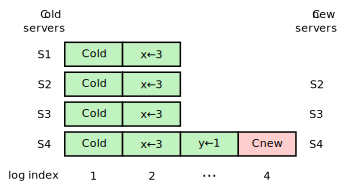
\includegraphics[scale=1]{membership/disruptive}
\vcaption[example of disruptive server]{
An example of how a server can be disruptive even before the \cnew{} log
entry has been committed, and the Pre-Vote phase doesn't help.
The figure shows the removal of S1 from a
four-server cluster. S4 is leader of the new
cluster and has created the \cnew{} entry in its log, but it hasn't yet
replicated that entry. Servers in the old cluster no longer receive
heartbeats from S4. Even before \cnew{} is committed, S1 can time out,
increment its term, and send this larger term number to the new cluster,
forcing S4 to step down. The Pre-Vote algorithm does not help, since
S1's log is as up-to-date as a majority of either cluster.
}
\label{fig:membership:disruptive}
\end{figure}

Unfortunately, the Pre-Vote phase does not solve the problem of
disruptive servers: there are situations where the disruptive server's
log is sufficiently up-to-date, but starting an election would still be
disruptive. Perhaps surprisingly, these can happen even before the
configuration change completes. For example,
Figure~\ref{fig:membership:disruptive} shows a server that is being
removed from a cluster. Once the leader creates the \cnew{} log entry,
the server being removed could be disruptive. The Pre-Vote check does
not help in this case, since the server being removed has a log that is
more up-to-date than a majority of either cluster. (Though the Pre-Vote
phase does not solve the problem of disruptive servers, it does turn out
to be a useful idea for improving the robustness of leader election in
general; see Chapter~\ref{leaderelection}.)

Because of this scenario, we now believe that no solution based on
comparing logs alone (such as the Pre-Vote check)
will be sufficient to tell if an election will be
disruptive. We cannot require a server to check the logs of
\emph{every} server in \cnew{} before starting an election,
since Raft must always be able to tolerate
faults. We also did not want to assume that a leader will reliably
replicate entries fast enough to move past the scenario shown in
Figure~\ref{fig:membership:disruptive} quickly; that might have worked
in practice, but it depends on stronger assumptions that we prefer to
avoid about the performance of finding where logs diverge and the
performance of replicating log entries.

Raft's solution uses heartbeats to determine when a valid leader exists.
In Raft, a leader is considered
active if it is able to maintain heartbeats to its followers (otherwise,
another server will start an election). Thus, servers should not be able
to disrupt a leader whose cluster is receiving heartbeats.
We modify the RequestVote RPC to achieve this: if a server receives a
RequestVote request within the minimum election timeout of hearing from a
current leader, it does not update its term or grant its vote. It can
either drop the request, reply with a vote denial, or delay the request;
the result is essentially the same. This does not affect normal
elections, where each server waits at least a minimum election timeout
before starting an election. However, it helps avoid disruptions from
servers not in \cnew{}: while a leader is able to get heartbeats to its
cluster, it will not be deposed by larger term numbers.

This change conflicts with the leadership transfer mechanism as
described in Chapter~\ref{basicraft}, in which a server legitimately
starts an election without waiting an election timeout.
In that case, RequestVote messages
should be processed by other servers even when they believe a current
cluster leader exists. Those RequestVote requests can include a special
flag to indicate this behavior (``I have permission to disrupt
the leader---it told me to!'').


\subsection{Availability argument}
\label{membership:availability:argument}

This section argues that the above solutions are sufficient to maintain
availability during membership changes. Since Raft's membership changes
are leader-based, we show that the algorithm will be able to maintain
and replace leaders during membership changes and that the leader(s) will
both service client requests and complete the configuration changes.
We assume, among other things, that a majority of the old configuration
is available (at least until \cnew{} is committed) and that a majority of
the new configuration is available.

\begin{enumerate}
%
\item A leader can be elected at all steps of the configuration change:
%
\begin{itemize}
%
\item If the available server with the most up-to-date log in the new
cluster has the \cnew{} entry, it can collect votes from a majority of
\cnew{} and become leader.
%
\item Otherwise, the \cnew{} entry must not yet be committed. The
available server with the most up-to-date log among both the old and new
clusters can collect votes from a majority of \cold{}
and a majority of \cnew{},
so no matter which configuration it uses, it can become leader.
%
\end{itemize}
%
\item A leader is maintained once elected, assuming its heartbeats get
through to its configuration, unless it intentionally steps down because
it is not in \cnew{} but has committed \cnew{}. 
%
\begin{itemize}
%
\item If a leader can reliably send heartbeats to its own configuration,
then neither it nor its followers will adopt a higher term: they will not time
out to start any new elections, and they will ignore any RequestVote
messages with a higher term from other servers. Thus, the leader will
not be forced to step down.
%
\item If a server that is not in \cnew{} commits the \cnew{} entry and
steps down, Raft will then elect a new leader. It is likely that this
new leader will be part of \cnew{}, allowing the configuration change to
complete. However, there is some (small) risk that the server that
stepped down might become leader again. If it was elected again, it
would confirm the commitment of the \cnew{} entry and soon step down,
and it is again likely that a server in \cnew{} would succeed the next
time.
%
\end{itemize}
%
\item The leader(s) will service client requests throughout the
configuration change.
%
\begin{itemize}
%
\item Leaders can continue to append client requests to their logs
throughout the change.
%
\item Since new servers are caught up before being added to the cluster,
a leader can advance its commit index and reply to
clients in a timely manner.
%
\end{itemize}
%
\item The leader(s) will progress towards and complete the configuration
change by committing \cnew{}, and, if necessary, stepping down to allow
a server in \cnew{} to become leader.
%
\end{enumerate}

\noindent
Therefore, under the above assumptions, the mechanisms described in this
section are sufficient to preserve availability during any membership
change.


\section{Arbitrary configuration changes using joint consensus}
\label{membership:arbitrary}

This section presents a more complex approach to cluster membership
changes that handles arbitrary changes to the configuration at one time.
For example, two servers can be added to a cluster at once, or all of
the servers in a five-server cluster can be replaced at once. This was
the first approach to membership changes that we came up with, and it is
described only for completeness. Now that we know about the simpler
single-server approach, we recommend that one instead, since handling
arbitrary changes requires extra complexity. Arbitrary changes are
typically the way membership changes are assumed to operate in the
literature, but we don't think this flexibility is needed in real
systems, where a series of single-server changes can change the cluster
membership to any desired configuration. 


To ensure safety across arbitrary configuration changes,
the cluster first switches to a transitional
configuration we call \emph{joint consensus}; once the joint consensus
has been committed, the system then transitions to the new
configuration. The joint consensus
combines both the old and new configurations:
\begin{itemize}
\item Log entries are replicated to all servers in both configurations.
\item Any server from either configuration may serve as leader.
\item Agreement (for elections and entry commitment) requires
separate majorities from \emph{both} the old and new configurations.
For example, when changing from a cluster of 3 servers to a
different cluster of 9 servers, agreement requires both 2 of
the 3 servers in the old configuration and 5 of the 9 servers in the new
configuration.
\end{itemize}
The joint consensus allows individual
servers to transition between configurations at different times
without compromising safety. Furthermore, joint
consensus allows the cluster to continue servicing client requests
throughout the configuration change.

\begin{figure}
\centering
\includegraphics[scale=.50]{membership/reconfigurationconf}
\vcaption[joint consensus timeline]{
Timeline for a configuration change using joint consensus. Dashed lines show configuration
entries that have been created but not committed, and solid lines
show the latest committed configuration entry. The leader first creates
the \cboth{} configuration entry in its log and commits it to \cboth{}
(a majority of \cold{} and a majority of \cnew{}).
Then it creates the \cnew{} entry and commits it to a majority of
\cnew{}. There is no point in time in which \cold{} and \cnew{} can
 both make decisions independently.
}
\label{fig:membership:reconfiguration}
\end{figure}

This approach extends the single-server membership change algorithm with an
intermediate log entry for the joint configuration;
Figure~\ref{fig:membership:reconfiguration} illustrates the
process. When the leader receives a request to
change the configuration from \cold{} to \cnew{}, it stores the
configuration for joint consensus (\cboth{} in the figure) as a log
entry and replicates that entry using the normal Raft mechanism. As with
the single-server configuration change algorithm, each server starts
using a new configuration as soon as it stores the configuration in its
log. This means that
the leader will use the rules of \cboth{} to determine when the log
entry for \cboth{} is committed. If the leader crashes, a new
leader may be chosen under either \cold{} or \cboth{}, depending
on whether the winning candidate has received \cboth{}.  In any
case, \cnew{} cannot make unilateral decisions during this period.

Once \cboth{} has been committed, neither \cold{} nor \cnew{}
can make decisions without approval of the other, and
the Leader Completeness Property ensures that only servers with the
\cboth{} log entry can be elected as leader.
It is now safe for the
leader to create a log entry describing \cnew{} and replicate it
to the cluster. Again, this configuration will take effect on
each server as soon as it is seen. When the \cnew{} log entry
has been committed under the rules of \cnew{}, the old configuration
is irrelevant and servers not in the
new configuration can be shut down. As shown in
Figure~\ref{fig:membership:reconfiguration},
there is no time when \cold{} and \cnew{} can both make
unilateral decisions; this guarantees safety.


The joint consensus approach could be generalized to allow a
configuration change to begin while a prior change was still in
progress. However, there would not be much practical advantage to doing
this. Instead, a leader rejects additional configuration changes when a
configuration change is already in progress (when its latest
configuration is not committed or is not a simple majority). Changes
that are rejected in this way can simply wait and try again later.

This joint consensus approach is more complex than the single-server
changes precisely because it requires transitioning to and from an
intermediate configuration. Joint configurations also require changes to
how all voting and commitment decisions are made; instead of simply
counting servers, the leader must check if the servers form a majority
of the old cluster and also form a majority of the new cluster.
Implementing this required finding and changing about six comparisons in
our Raft implementation~\cite{logcabin}.


\section{System integration}
\label{membership:system}

Raft implementations may expose the cluster membership change mechanism
described in this chapter in different ways. For example, the AddServer
and RemoveServer RPCs in Figure~\ref{fig:membership:cheatsheet2} can be
invoked by administrators directly, or they can be invoked by a script
that uses a series of single-server steps to change the configuration in
arbitrary ways.

It may be desirable to invoke membership changes automatically in
response to events like server failures. However, this should only be
done according to a reasonable policy. For example, it can be dangerous
for the cluster to automatically remove failed servers, as it could then
be left with too few replicas to satisfy the intended durability and
fault-tolerance requirements. One reasonable approach is to have the
system administrator configure a desired cluster size, and within that
constraint, available servers could automatically replace failed
servers.

When making cluster membership changes that require multiple
single-server steps, it is preferable to add servers before removing
servers. For example, to replace a server in a three-server cluster,
adding one server and then removing the other allows the system to
handle one server failure at all times throughout the process. However,
if one server was first removed before the other was added, the system
would temporarily not be able to mask any failures (since two-server
clusters require both servers to be available).

Membership changes motivate a different approach to bootstrapping a
cluster. Without dynamic membership, each server simply has a static
file listing the configuration. With dynamic membership changes, the
static configuration file is no longer needed, since the system manages
configurations in the Raft log; it is also potentially error-prone
(e.g., with which configuration should a new server be initialized?).
Instead, we recommend that the very first time a cluster is created, one
server is initialized with a configuration entry as the first entry in
its log. This configuration lists only that one server; it alone forms a
majority of its configuration, so it can consider this configuration
committed. Other servers from then on should be initialized with empty
logs; they are added to the cluster and learn of the current
configuration through the membership change mechanism.

Membership changes also necessitate a dynamic approach for clients to
find the cluster; this is discussed in Chapter~\ref{clients}.

\section{Conclusion}

This chapter described an extension to Raft for handling cluster
membership changes automatically. This is an important part of a
complete consensus-based system, since fault-tolerance requirements
can change over time, and failed servers eventually need to be replaced.

The consensus algorithm must fundamentally be involved in preserving
safety across configuration changes, since a new configuration affects
the meaning of ``majority''. This chapter presented a simple approach
that adds or removes a single server at a time. These operations preserve
safety simply, since at least one server overlaps any majority during
the change. Multiple single-server changes may be composed to modify the
cluster more drastically. Raft allows the cluster to continue operating
normally during membership changes.

Preserving availability during configuration changes requires handling
several non-trivial issues. In particular, the issue of a server not in
the new configuration disrupting valid cluster leaders was surprisingly
subtle; we struggled with several insufficient solutions based on log
comparisons before settling on a working solution based on heartbeats.

\chapter{Log compaction}
\label{compaction}


Raft's log grows during normal operation as it incorporates more client
requests. As it grows larger, it occupies more space and takes more time
to replay. Without some way to compact the log, this will eventually
cause availability problems: servers will either run out of space, or
they will take too long to start. Thus, some form of log compaction is
necessary for any practical system.

The general idea of log compaction is that much of the information in
the log becomes obsolete over time and can be discarded. For example, an
operation that sets $x$ to 2 is obsolete if a later operation sets $x$
to 3. Once log entries have been committed and applied to the
state machine, the intermediate states and operations used to arrive at
the current state are no longer needed, and they can be compacted away.

Unlike the core Raft algorithm and membership changes, different systems
will have different needs when it comes to log compaction. There is no
one-size-fits-all solution to log compaction for a couple of reasons.
First, different systems may choose to trade off simplicity and
performance to varying degrees. Second, the state machine must be
intimately involved in log compaction, and state machines differ
substantially in size and in whether they are based on disk or volatile memory.

\begin{figure*}
\centering
\includegraphics[scale=0.95]{compaction/rules}
\vcaption[summary of approaches]{
The figure shows how various approaches to log compaction can be used in
Raft. Details for log-structured merge trees in the figure are based
on LevelDB~\cite{leveldb:compactions}, and details for log cleaning are
based on RAMCloud~\cite{Rumble:2014}; rules for managing deletions are
omitted.
}
\label{fig:compaction:rules}
\end{figure*}

The goal of this chapter is to discuss a variety of approaches to log
compaction. In each approach, most of the responsibility of log
compaction falls on the state machine, which is in charge of writing the
state to disk and compacting the state. State machines can achieve this
in different ways, which are described throughout the chapter and
summarized in Figure~\ref{fig:compaction:rules}:
%
\begin{itemize}
%
\item
%
Snapshotting for memory-based state machines is conceptually the
simplest approach. In snapshotting, the entire current system state is
written to a \emph{snapshot} on stable storage, then the entire log up
to that point is discarded. Snapshotting is used in
Chubby~\cite{Burrows:2006, Chandra:2007} and ZooKeeper~\cite{Hunt:2010},
and we have implemented snapshotting in LogCabin. Snapshotting is the
approach presented in the most depth in this chapter,
in Section~\ref{compaction:memsnapshot}.
%
\item
%
With disk-based state machines, a recent copy of the system state is
maintained on disk as part of normal operation. Thus, the Raft log can
be discarded as soon as the state machine reflects writes to disk,
and snapshotting is used only when sending consistent disk images to
other servers
(Section~\ref{compaction:disksnapshot}).
%
\item
%
Incremental approaches to log compaction, such as log cleaning and
log-structured merge trees, are presented in
Section~\ref{compaction:incremental}. These approaches write to disk
efficiently, and they utilize resources evenly over time.
%
\item
%
Finally, Section~\ref{compaction:leader} discusses an approach to log
compaction that minimizes the mechanism required by storing snapshots
directly in the log. Though easier to implement, this approach is only
suitable for very small state machines.
%
\end{itemize}
%
LogCabin currently only implements the memory-based snapshotting
approach (it embeds a memory-based state machine).

The various approaches to compaction share several core concepts. First,
instead of centralizing compaction decisions on the leader, each server
compacts the
committed prefix of its log independently. This avoids having the leader
transmit data to followers that already have the data in their logs. It also
helps modularity: most of the complexity of log compaction is
contained within the state machine and does not interact much with Raft
itself. This helps keep overall system complexity to a
minimum: the complexity of Raft adds to, rather than multiplies with,
the complexity of log compaction. Alternative approaches that centralize compaction
responsibilities on a leader are discussed further in
Section~\ref{compaction:leader} (and for very small state machines, a
leader-based approach may be better).

Second, the basic interaction between the state machine and Raft
involves transferring responsibility for a prefix of the log from Raft
to the state machine.
Sooner or later after applying entries, the state machine reflects those
entries to disk in a way that can recover the current system state.
Once it has done so, it tells Raft to discard the corresponding
prefix of the log. 
Before Raft can give up responsibility for the log prefix,
it must save some of its own state describing the log prefix.
Specifically, Raft retains the index and term of the last entry it
discarded; this anchors the rest of the log in place after the state
machine's state and allows the AppendEntries consistency check to
continue to work (it needs the index and term for the entry preceding
the first entry in the log). Raft also retains the latest configuration
from the discarded log prefix in order to support cluster membership
changes.

Third, once Raft has discarded a prefix of the log, the state machine
takes on two new responsibilities. If the server restarts, the state
machine will need to load the state corresponding to the discarded log
entries from disk before it can apply any entries from the Raft log.
In addition, the state machine may need to produce a consistent image of
the state so that it can be sent to a slow follower
(one whose log is far behind the leader's). It is not feasible
to defer compaction  until log entries have been ``fully replicated'' to
every member in the cluster, since a minority of slow followers must not
keep the cluster from being fully available, and new servers can be
added to the cluster at any time. Thus, slow followers or new servers
will occasionally need to receive their initial states over the network.
Raft detects this when the next entry needed in AppendEntries has
already been discarded in the leader's log. In this case, the state
machine must provide a consistent image of the state, which the leader
then sends to the follower.



\section{Snapshotting memory-based state machines}
\label{compaction:memsnapshot}

The first approach to snapshotting applies when the state machine's data
structures are kept in memory. This is a reasonable choice for state
machines with datasets in the gigabytes or tens of gigabytes. It
enables operations to complete quickly, since they never have to fetch
data from disk; it is also easy to program, since rich data
structures can be used and every operation can run to completion
(without blocking for I/O).

\begin{figure}
\centering
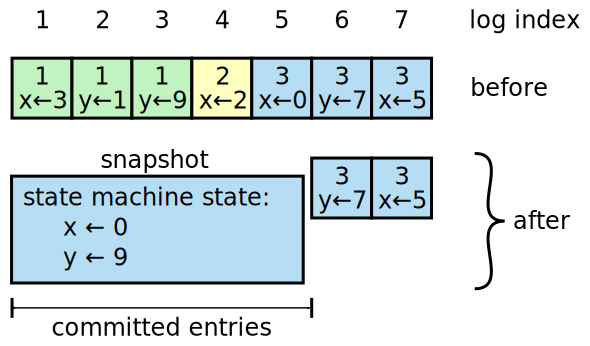
\includegraphics[scale=.50]{compaction/snapshot}
\vcaption[memory-based snapshotting approach]{
A server replaces the committed entries in its log (indexes 1 through 5)
with a new snapshot, which stores just the current state (variables
$x$ and $y$ in this example). Before discarding entries 1 though 5,
Raft saves the snapshot's last included
index (5) and term (3) to position the snapshot in the log preceding
entry 6.
}
\label{fig:compaction:snapshot}
\end{figure}

Figure~\ref{fig:compaction:snapshot} shows the basic idea of
snapshotting in Raft when the state machine is kept in memory. Each
server takes snapshots independently, covering just the committed
entries in its log. Most of the work in snapshotting involves
serializing the state machine's current state, and this is specific to a
particular state machine implementation. For example, LogCabin's
state machine uses a tree as its primary data structure; it serializes
this tree using a pre-order depth-first traversal (so that when
applying the snapshot, parent nodes are created before their children).
State machines must also serialize the information they keep for
providing linearizability to clients (see Chapter~\ref{clients}).

Once the state machine completes writing a snapshot, the log can be
truncated. Raft first stores the state it needs for a restart:
the index and term of the last entry included in the snapshot and the
latest configuration as of that index. Then it discards the prefix of
its log up through that index. Any previous snapshots can also be
discarded, as they are no longer useful.

\begin{figure}
\centering
\includegraphics[scale=1.0]{compaction/cheatsheet}
\vcaption[InstallSnapshot RPC]{
Leaders invoke the InstallSnapshot RPC to send snapshots to slow
followers. Leaders resort to sending a snapshot only when they
have already discarded the next log entry needed to
replicate entries to the follower with AppendEntries.
They split the snapshot into chunks for transmission. Among other
benefits, this gives the follower a sign of life with each chunk, so it
can reset its election timer. Each chunk is sent in order, which
simplifies writing the file to disk.
The RPC includes the state needed for Raft to load the snapshot on a
restart: the index and term of the last entry covered by the snapshot,
and the latest configuration at that point.
}
\label{fig:compaction:cheatsheet}
\end{figure}

As introduced above, the leader may occasionally need to send its state
to slow followers and to new servers that are joining the cluster. In
snapshotting, this state is just the latest snapshot, which the leader
transfers using a new RPC called InstallSnapshot, as shown in
Figure~\ref{fig:compaction:cheatsheet}.
When a follower receives a snapshot with this RPC, it must decide
what to do with its existing log entries.
Usually the snapshot will
contain new information not already in the follower's log.
In this case, the follower discards its entire log; it is all
superseded by the snapshot and may possibly have uncommitted entries
that conflict with the snapshot. If, instead, the follower receives a
snapshot that describes a prefix of its log (due to retransmission or by
mistake), then log entries covered by the snapshot are deleted but
entries following the snapshot are still valid and must be retained.

The remainder of this section discusses secondary issues for
snapshotting memory-based state machines:
%
\begin{compactitem}
%
\item Section~\ref{compaction:memsnapshot:concurrent} discusses how to
produce snapshots in parallel with normal operations, to minimize their
effects on clients;
%
\item Section~\ref{compaction:memsnapshot:when} discusses when to take a
snapshot, balancing the space usage and the overhead of snapshotting; and
%
\item Section~\ref{compaction:memsnapshot:implementation} discusses the
issues that arise in implementing snapshotting.
%
\end{compactitem}

\subsection{Snapshotting concurrently}
\label{compaction:memsnapshot:concurrent}

Creating a snapshot can take a long time, both in serializing
the state and in writing it to disk. For example, copying
\SI{10}{\giga\byte} of
memory takes about one second on today's servers, and serializing it
will usually take much longer: even a solid state disk
can only write about \SI{500}{\mega\byte} in one second.
Thus, both serializing and
writing snapshots must be concurrent with normal operations to avoid
availability gaps.

Fortunately, copy-on-write techniques allow new updates to be applied
without impacting the snapshot being written.
There are two approaches to this:
%
\begin{itemize}
%
\item State machines can be built with immutable (functional) data
structures to support this. Because state machine commands would not modify
the state in place, a snapshotting task could keep a reference to
some prior state and write it consistently into a snapshot.
\item
Alternatively, the operating system's copy-on-write support can be used
(where the programming environment allows it).
On Linux for example, in-memory state machines can use \emph{fork} to make a
copy of the server's entire address space. Then, the child process can
write out the state machine's state and exit, all while the parent
process continues servicing requests. The LogCabin implementation
currently uses this approach.
\end{itemize}

Servers require additional memory for snapshotting concurrently, which should be
planned for and managed. It is essential for state machines to have a
streaming interface to the snapshot file, so that the snapshot does not
have to be staged entirely in memory while it is created. Still,
copy-on-write requires extra memory proportional to the fraction of the
state machine state that is changed during the snapshotting process. Moreover, relying on
the operating system for copy-on-write will typically use even more
memory due to false sharing (for example, if two unrelated data items
happen to be on the same page of memory, the second item will be
duplicated even when only the first has changed). In the unfortunate
event that memory capacity is exhausted during snapshotting, a server should
stop accepting new log entries until it completes its snapshot; this
would temporarily sacrifice the server's availability (the cluster might
still remain available), but at least it would allow the server to
recover. It is better not to abort the snapshot and retry later,
since the next attempts might also face the same problem.
(LogCabin uses a streaming interface to disk, but it does not currently
handle memory exhaustion gracefully.)


\subsection{When to snapshot}
\label{compaction:memsnapshot:when}

Servers must decide when to snapshot. If a server snapshots too often,
it wastes disk bandwidth and other resources; if it snapshots too
infrequently, it risks exhausting its storage capacity, and it increases
the time required to replay the log during restarts.

One simple strategy is to take a snapshot when the log reaches a fixed
size in bytes. If this size is set to be significantly larger than the
expected size of a snapshot, then the disk bandwidth overhead for
snapshotting will be small. However, this can result in needlessly large
logs for small state machines.

A better approach involves comparing the snapshot's size with the log's
size. If the snapshot will be many times smaller than the log, it is
probably worthwhile to take a snapshot. However, calculating the size of
a snapshot before it is taken can be difficult and burdensome, imposing
a significant bookkeeping burden for the state machine, or requiring
almost as much work as actually taking a snapshot to compute the size
dynamically. Compressing snapshot files also results in space and
bandwidth savings, but it is hard to predict how large the compressed
output will be.

Fortunately, using the size of the \emph{previous} snapshot rather than
the size of the next one results in reasonable behavior. Servers take a
snapshot once the size of the log
exceeds the size of the previous snapshot times a configurable
\emph{expansion factor}. The expansion factor trades off disk bandwidth
for space utilization. For example, an expansion factor of 4 results in
about 20\% of the disk's bandwidth being used towards snapshotting (for
every 1 byte of snapshot, 4 bytes of log entries will be written), and
requires about 6 times the disk capacity as that needed to store a
single copy of the state (the old snapshot, a log 4 times bigger than
that, and the new snapshot being written).

Snapshotting still creates a burst of CPU and disk bandwidth usage that
might impact client performance. This can be mitigated with additional
hardware; for example, a second disk drive can be used to provide the
additional disk bandwidth.

It may also be possible to schedule snapshots in a way that client
requests never wait on a server that is snapshotting. In this approach,
servers would coordinate so that only up to a minority of the servers in
the cluster would snapshot at any one time (when possible). Because Raft
only requires a majority of servers to commit log entries, the minority of
snapshotting servers would normally have no adverse effect on clients.
When a leader wished to snapshot, it would step down first,
allowing another server to manage the cluster in the meantime. If this
approach was sufficiently reliable, it could also eliminate the need to
snapshot concurrently; servers could just be unavailable while they took
their snapshots (though they would count against the cluster's
ability to mask failures). This is an exciting opportunity for future
work because of its potential to both improve overall system performance
and reduce mechanism. 

%


\subsection{Implementation concerns}
\label{compaction:memsnapshot:implementation}

This section reviews the major components needed for a snapshotting
implementation and discusses the difficulties with implementing them:
%
\begin{itemize}
%
\item \textbf{Saving and loading snapshots:}
%
Saving a snapshot involves serializing the state machine's state and
writing that data out to a file, while loading is the reverse process.
We found this to be fairly straightforward, although it was somewhat
tedious to serialize the various types of data objects from their native
representations. A streaming interface from the state machine to a file
on disk is useful to avoid buffering the entire state machine state in
memory; it may also be beneficial to compress the stream and apply a
checksum to it.
LogCabin writes each snapshot to a temporary file first, then renames
the file when writing is complete and has been flushed to disk; this
ensures that no server loads a partially written snapshot on startup.

%
\item \textbf{Transferring snapshots:}
%
Transferring snapshots involves implementing the leader and follower
sides of the InstallSnapshot RPC. This is fairly straightforward and may
be able to share some code with saving snapshots to and loading
snapshots from disk.
The performance of this transfer is usually not very important (a
follower that needs this state has not been participating in the
commitment of entries, so it is probably not needed soon; on the other
hand, if the cluster suffers additional failures,
it may need to catch up the follower to restore availability).
%
\item \textbf{Eliminating unsafe log accesses and discarding log
entries:}
%
We originally designed LogCabin without worrying about
log compaction, so the code assumed that if entry $i$ was present in the
log, entries $1$ through $i - 1$ would also be present. This is no
longer true with log compaction; for example, when determining the term
for the previous entry in the AppendEntries RPC, that entry might have
been discarded.
Removing these assumptions throughout the code required careful
reasoning and testing. This would have been easier with help from a more
powerful type system, if the compiler could enforce that every access to
the log also handled the case that the index was out of bounds.
Once we had made all the log accesses safe, discarding the prefix of
the log was straightforward. Until this point, we could only test the
saving, loading, and transferring snapshots in isolation, but when log entries can be safely
discarded, these can all start to be exercised in
system-wide tests.
%
\item \textbf{Snapshotting concurrently with copy-on-write:}
%
Snapshotting concurrently may require reworking the state machine or
leveraging the operating system's fork operation. LogCabin currently
uses fork, which interacts poorly with threads and C++
destructors; getting this to work correctly presented some
difficulty. However, it is a small amount of code and completely
eliminates the need to modify the state machine's data structures, so we
think it was the right approach.
%
\item \textbf{Deciding when to snapshot:}
%
We recommend taking snapshots after applying every log entry during
development, since that can help catch bugs quickly. Once the
implementation is complete, a more useful policy of when to snapshot
should be added (e.g., using statistics about the size of Raft log and the
size of the last snapshot).
%
\end{itemize}

We found piecewise development and testing of snapshotting to be
challenging. Most of these components must be in place before it is
possible to discard log entries, but only then will many of the new code
paths be exercised in system-wide tests. Thus, implementers should
consider the order in which to implement and test these components carefully.

\section{Snapshotting disk-based state machines}
\label{compaction:disksnapshot}

This section discusses a snapshotting approach for large state machines
(on the order of tens or hundreds of gigabytes) that use disk as their
primary location of record. 
These state machines behave differently in that they always have a copy
of the state ready on disk in case of a crash.
Applying each entry from the Raft log mutates
the on-disk state and effectively arrives at a new snapshot. Thus, once
an entry is applied, it can be discarded from the Raft log.
(State machines can also buffer writes in memory in hopes of achieving
better disk efficiency; once they are written to disk, the corresponding
entries can be discarded from the Raft log.)

The main problem with disk-based state machines is that
mutating state on disk can lead to poor performance. Without write
buffering, it requires one or more random disk writes for every command
applied, which can limit the system's overall write throughput (and
write buffering might not help much).
Section~\ref{compaction:incremental} discusses incremental approaches to
log compaction which write to disk more efficiently with large,
sequential writes.

Disk-based state machines must be able to provide a consistent
snapshot of the disk for the purpose of transmitting it to slow
followers. Although they always have a snapshot on disk, they are
continuously modifying it. Thus, they still require copy-on-write
techniques to retain a consistent snapshot for a long enough period to
transmit it. Fortunately, disk formats are almost always divided into
logical blocks, so implementing copy-on-write in the state machine
should be straightforward. Disk-based state machines can also rely on
operating system support for their snapshots. For example, LVM (logical
volume management) on Linux can be used to create snapshots of entire
disk partitions~\cite{lvm}, and some recent file systems allow
snapshotting individual directories~\cite{btrfssnapshots}.

Copying a snapshot of a disk image can take a long time, and as
modifications to the disk accumulate, so does the extra disk usage
required to retain the snapshot.
Although we haven't implemented disk-based snapshotting,
we speculate that disk-based state
machines could avoid most of this overhead by transmitting their disk
contents with the following algorithm:
%
\begin{enumerate}
%
\item For each disk block, track the time it was last modified.
%
\item While continuing normal operation, transmit the entire disk
contents to a follower block by block. During this process, no extra
disk space is used on the leader. Since blocks are being modified
concurrently, this is likely to result in an inconsistent disk image on
the follower. As each block is transferred from the leader, note its
last modification time.
%
\item Take a copy-on-write snapshot of the disk contents. Once this is
taken, the leader has a consistent copy of its disk contents, but
additional disk space is used as modifications to the disk occur due to
continued client operations.
%
\item Retransmit only the disk blocks that were modified between when
they were first transmitted in Step~2 and when the snapshot was taken in
Step~3.
%
\end{enumerate}
%
Hopefully, most of the blocks of the consistent snapshot will have
already been transmitted by the time it is created in Step~3. If that is
the case, the transfer in Step~4 will proceed quickly: the additional
disk capacity used to retain the snapshot on the leader during Step~4
will be low, and the additional network bandwidth used during Step~4 to
retransmit modified blocks will also be low.





\section{Incremental cleaning approaches}
\label{compaction:incremental}

Incremental approaches to compaction, such as log
cleaning~\cite{Rosenblum:1992,Rumble:2014} and log-structured merge
trees~\cite{ONeil:1996,Chang:2006} (LSM trees), are also possible.
Although they are more complex than snapshotting, incremental
approaches have several desirable features:
%
\begin{itemize}
%
\item They operate on only a fraction of the data at once, so they
spread the load of compaction evenly over time.
%
\item They write to disk efficiently, both in normal operation and
while compacting. They use large, sequential writes in both cases.
Incremental approaches also selectively compact parts of the disk
with the most reclaimable space, so they write less data to disk than
snapshotting for memory-based state machines (which rewrites all of disk
on every snapshot).
%
\item They can transfer consistent state snapshots fairly easily
because they do not modify regions of disk in place.
%
\end{itemize}
%
Section~\ref{compaction:incremental:cleaning} and
Section~\ref{compaction:incremental:lsmtrees}
first describe the basics of log cleaning and LSM trees in
general. Then, Section~\ref{compaction:incremental:raft}
discusses how they could be applied to Raft.

\subsection{Basics of log cleaning}
\label{compaction:incremental:cleaning}

Log cleaning was introduced in the context of log-structured file
systems~\cite{Rosenblum:1992} and has recently been proposed for
in-memory storage systems such as RAMCloud~\cite{Rumble:2014}.
In principle, log cleaning can be used for any type of data structure,
though some would be harder to implement efficiently than others.

Log cleaning maintains the log as the place of record for the system's
state. The layout is optimized for sequential writing, and it makes read
operations effectively random access. Thus, indexing structures are
needed to locate data items to read.

In log cleaning, the log is split into consecutive regions called
\emph{segments}. Each pass of the log cleaner compacts the log using a
three-step algorithm:
%
\begin{enumerate}
%
\item It first selects segments to clean that have accumulated a large
fraction of obsolete entries.
%
\item It then copies the \emph{live} entries (those that contribute to
the current system state) from those segments to the head of the log.
%
\item Finally, it frees the storage space for the segments, making
that space available for new segments.
%
\end{enumerate}
%
To minimize the effect on normal operation, this process can be done
concurrently~\cite{Rumble:2014}.

As a result of copying the live entries forwards to the head of the log,
the entries get to be out of order for replay. The entries can include
additional information (e.g., version numbers) to recreate the correct
ordering when the log is applied.

The policy of which segments are selected for cleaning has a big impact
on performance; prior work proposes a cost-benefit policy that factors
in not only the amount of space utilized by live entries but also how
long those entries are likely to remain
live~\cite{Rosenblum:1992,Rumble:2014}.

Determining whether entries are live is the state machine's
responsibility. For example, in a key-value store, a log entry to set a
key to a particular value is live if the key exists and is currently set
to the given value. Determining whether a log entry that deletes a key
is live is more subtle: it is live as long as any prior entries setting that key
are present in the log. RAMCloud
preserves deletion commands (called tombstones) as
necessary~\cite{Rumble:2014}, but another approach is to periodically write
out a summary of the keys that
\emph{are} present in the current state, then all log entries regarding
keys not listed are not live. Key-value stores are a fairly simple
example; other state machines are possible, but unfortunately,
determining liveness will be different for each.

\subsection{Basics of log-structured merge trees}
\label{compaction:incremental:lsmtrees}


Log-structured merge trees (LSM trees) were first described by
O'Neil~\cite{ONeil:1996} and were later popularized in distributed
systems by BigTable~\cite{Chang:2006}. They are used in systems such as
Apache Cassandra~\cite{Cassandra} and HyperDex~\cite{Escriva:2012} and
are available as libraries such as LevelDB~\cite{leveldb} and its forks
(e.g., RocksDB~\cite{rocksdb} and HyperLevelDB~\cite{hyperleveldb}).

LSM trees are tree-like data structures that store ordered key-value
pairs. At a high level, they use disk similarly to log cleaning
approaches: they write in large sequential strides and do not modify
data on disk in place. However, instead of maintaining all state in the
log, LSM trees reorganize the state for better random access.

A typical LSM tree keeps recently written keys in a small log on disk.
When the log reaches a fixed size, it is sorted by key and written to
a file called a \emph{run} in sorted order.
Runs are never modified in place, but a compaction process periodically
merges multiple runs together, producing new runs and discarding the old
ones. The merge is reminiscent of merge sort; when a key is in multiple
input runs, only the latest version is kept, so the produced runs are
more compact. The compaction strategy used in LevelDB is summarized in
Figure~\ref{fig:compaction:rules}; it segregates runs by age for
efficiency (similar to log cleaning).

During normal operation, the state machine can operate on this data
directly. To read a key, it first checks to see if that key was modified
recently in its log, then checks each run. To avoid checking every run
for a key on every lookup, some systems create a bloom filter for each
run (a compact data structure which can say with certainty in some cases
that a key does not appear in a run, though it may sometimes require
searching a run even when a key is not present).

\subsection{Log cleaning and log-structured merge trees in Raft}
\label{compaction:incremental:raft}

We have not attempted to implement log cleaning or LSM trees in Raft,
but we speculate that both would work well. Applying LSM trees to Raft
appears to be fairly straightforward. Because the Raft log already
stores recent entries durably on disk, the LSM tree can keep recent data
in a more convenient tree format in memory. This would be fast for servicing
lookups, and when the Raft log reached a fixed size, the tree would already
be in sorted order to write to disk as a new run. Transferring the state
from the leader to a slow follower requires sending all the runs to the
follower (but not the in-memory tree); fortunately, runs are immutable,
so there is no concern of the runs being modified during the transfer.

\begin{figure}
\centering

\begin{subfigure}{\textwidth}
\centering
\includegraphics[scale=.45]{compaction/cleaningdirect}
\caption{
Cleaning the Raft log directly would lead to many holes, which would
add significant complexity to Raft and its interaction with the state
machine.
}
\label{fig:compaction:incremental:cleaningdirect}
\end{subfigure}

\vspace{2ex}

\begin{subfigure}{\textwidth}
\centering
\includegraphics[scale=.45]{compaction/cleaningtwologs}
\caption{
The state machine could instead structure its own data as a log and
clean that log independently, without involving Raft.
}
\label{fig:compaction:incremental:cleaningtwologs}
\end{subfigure}

\vcaption[approaches to log cleaning in Raft]{
Two possible approaches to log cleaning in Raft.
}
\end{figure}

Applying log cleaning to Raft is less obvious. We first considered an
approach in which the Raft log was divided into segments and cleaned
(see Figure~\ref{fig:compaction:incremental:cleaningdirect}).
Unfortunately, cleaning would place a lot of holes in the log where
segments were freed, which would require a modified approach to log
replication. We think this approach could be made to work, but it adds
significant complexity to Raft and its interaction with the state
machine. Moreover, since only the leader can append to the Raft log,
cleaning would need to be leader-based, which would waste the leader's
network bandwidth (this is discussed further in
Section~\ref{compaction:leader}).


A better approach would be to handle log cleaning similarly to LSM
trees: Raft would keep a contiguous log for recent changes, and the
state machine would keep its own state as a log, but these logs would be
logically distinct (see
Figure~\ref{fig:compaction:incremental:cleaningtwologs}). When the Raft
log grew to a fixed size, its new entries would be written as a new
segment in the state machine's log, and the corresponding prefix of the
Raft log would be discarded. Segments in the state machine would be
cleaned independently on each server, and the Raft log would remain
entirely unaffected by this. We prefer this approach over cleaning the
Raft log directly, since the complexity of log cleaning is encapsulated
entirely in the state machine (the interface between the state machine
and Raft remains simple), and servers can clean independently.

As described, this approach would require the state machine to write all of
Raft's log entries into its own log (though it could do so in large
batches). This additional copy could be optimized away by directly
moving a file consisting of log entries from Raft's log and
incorporating that file into the state machine's data structures.
This could be a helpful optimization for performance-critical systems, but
unfortunately, it would more tightly couple the state machine and the
Raft module, since the state machine would need to understand the
on-disk representation of the Raft log.

\section{Alternative: leader-based approaches}
\label{compaction:leader}

The log compaction approaches presented in this chapter depart from Raft's
strong leader principle, since servers compact their logs without the
knowledge of the leader. However, we think this departure is justified.
While having a leader helps avoid conflicting decisions in reaching
consensus, consensus has already been reached when snapshotting, so no
decisions conflict. Data still only flows from leaders to followers,
but followers can now reorganize their data independently.

We also considered leader-based approaches to log compaction, but any
benefits are usually outweighed by performance considerations.
It would be wasteful for the leader to compact its log, then send the result
to the followers, when they could just as well compact their own logs
independently.
Sending the redundant state to each follower would waste network
bandwidth and slow the compaction process. Each follower already has the
information needed to compact its own state, and the leader's outbound
network bandwidth is usually Raft's most precious (bottleneck) resource.
For memory-based snapshots, it is typically much cheaper for a server to
produce a snapshot from its local state than it is to send and receive
one over the network. For incremental compaction approaches, this depends
a bit more on the hardware configuration, but we also expect independent
compaction to be cheaper.

\subsection{Storing snapshots in the log}

\begin{figure}
\centering
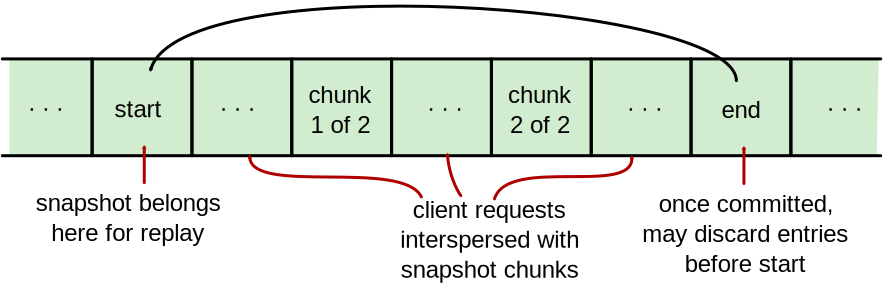
\includegraphics[scale=0.5]{compaction/logbased}
\vcaption[alternative: snapshot stored in log]{
A leader-based approach that stores the snapshot in chunks in the log,
interleaved with client requests. The snapshotting process is started at
the \emph{start} entry, and it completes by the \emph{end} entry.
The snapshot is stored in several log entries between \emph{start} and
\emph{end}.
%
So that client requests can proceed in parallel with snapshotting, each
entry is limited in size, and the rate at which the entries are appended
to the log is limited: the next snapshot chunk is only appended to the
log when the leader learns that the previous snapshot chunk has been
committed.
%
Once each server learns that the \emph{end} entry is committed, it can
discard the entries in its log up to the corresponding \emph{start}
entry. Replaying the log requires a two pass algorithm: the last
complete snapshot is applied first, then the client requests after the
snapshot's \emph{start} entry are applied.
}
\label{fig:compaction:logbased}
\end{figure}

One possible benefit to leader-based approaches is that, if all the
system state could be stored in the log, then new mechanisms to
replicate and persist the state would not be needed. Thus, we considered
a leader-based approach to snapshotting in which the leader would create
a snapshot and store the snapshot as entries in the Raft log, as shown
in Figure~\ref{fig:compaction:logbased}. The leader would then send this
snapshot to each of its followers using the AppendEntries RPC. 
To reduce any disruption on normal operation, each snapshot would be
split into many entries and interleaved with normal client commands in
the log.

This would achieve better economy of mechanism than storing the snapshot
outside the log, since servers would not need separate mechanisms to
transfer snapshots or persist them (they would be replicated and persisted
just like other log entries). However, in addition to wasting network
bandwidth for followers that could just as easily produce their own
snapshots, this has a serious problem. If a leader fails in the middle
of creating a snapshot, it leaves a partial snapshot in the servers'
logs. In principle this could happen repeatedly and exhaust servers'
storage capacity with garbage accumulated from numerous failed
snapshotting attempts. Thus, we don't think this mechanism is viable in
practice.



\subsection{Leader-based approach for very small state machines}

For very small state machines, storing the snapshot in the log not only
becomes viable but can also be simplified significantly. If the snapshot
is small enough (up to about one megabyte), it can fit comfortably in a
single log entry without interrupting normal operation for too long. To
compact the servers' logs in this way, the leader would:
\vspace{2ex}
\begin{compactenum}
\item Stop accepting new client requests;
\item Wait for all entries in its log to be committed and its state
machine to have applied all entries in its log;
\item Take a snapshot (synchronously);
\item Append the snapshot into a single log entry at the end of its log; and
\item Resume accepting new client requests.
\end{compactenum}
Once each server learned that the snapshot entry was committed, it could
discard every entry before the snapshot in its log. This approach would
cause a small availability gap while client requests were stopped and the
snapshot entry was transferred, but its impact would be limited for very
small state machines.

This simpler approach avoids
the implementation effort of persisting snapshots outside the log,
transferring them using a new RPC, and snapshotting concurrently.
However, successful systems tend to be used more than their original
designers intended, and this approach would not work well for larger
state machines.

\section{Conclusion}
\label{compaction:conclusion}

This chapter discussed several approaches to log compaction in Raft,
which are summarized in Figure~\ref{fig:compaction:rules}. Different
approaches are suitable for different systems, depending on the size of
the state machine, the level of performance required, and the amount of
complexity budgeted.
Raft supports a wide variety of approaches that share a common
conceptual framework:
%
\begin{itemize}
%
\item Each server compacts the committed prefix of its log
independently.
%
\item The basic interaction between the state machine and Raft involves
transferring responsibility for a prefix of the log from Raft to the
state machine. Once the state machine has applied commands to disk, it
instructs Raft to discard the corresponding prefix of the log. Raft
retains the index and term of the last entry it discarded, along with
the latest configuration as of that index.
%
\item Once Raft has discarded a prefix of the log, the state machine
takes on two new responsibilities: loading the state on a restart and
providing a consistent image to transfer to a slow follower.
%
\end{itemize}

Snapshotting for memory-based state machines is used successfully in
several production systems, including Chubby and ZooKeeper,
and we have implemented this approach in LogCabin. Although
operating on an in-memory data structure is fast for most operations,
performance during the snapshotting process may be significantly
impacted. Snapshotting
concurrently helps to hide the resource usage, and in the future,
scheduling servers across the cluster to snapshot at different times
might keep snapshotting from affecting clients at all.

Disk-based state machines that mutate their state in place are
conceptually simple. They still require copy-on-write for transferring a
consistent disk image to other servers, but this may be a small burden
with disks, which naturally split into blocks. However, random disk writes
during normal operation tend to be slow, so this approach will limit the
system's write throughput.

Ultimately, incremental approaches can be the most efficient form of
compaction. By
operating on small pieces of the state at a time, they can limit bursts
in resource usage (and they can also compact concurrently). They can
also avoid writing the same data out to disk repeatedly; stable
data should make its way to a region of disk that does not get
compacted often. While implementing incremental compaction can be complex, this
complexity can be offloaded to a library such as LevelDB. Moreover, by
keeping data structures in memory and caching more of the disk in
memory, the performance for client operations with incremental
compaction can approach that of memory-based state machines.


\chapter{Client interaction}
\label{clients}

\begin{figure}
\centering
\includegraphics[scale=0.95]{clients/cheatsheet}
\vcaption[summary of RPCs]{
Clients invoke the ClientRequest RPC to modify the replicated state;
they
invoke the ClientQuery RPC to query the replicated state. New clients
receive their client identifier using a RegisterClient RPC, which helps
identify when session information needed for linearizability has been discarded.
In the figure, servers that are not leaders
redirect clients to the leader, and read-only requests are serviced
without relying on clocks for linearizability (the text presents
alternatives).
Section numbers such as \S\ref{clients:linearizability} indicate where
particular features are discussed.
}
\label{fig:clients:cheatsheet}
\end{figure}

This chapter describes several issues in how clients interact with a
Raft-based replicated state machine:
\begin{compactitem}
\item Section~\ref{clients:findcluster} describes how clients find the
cluster, even when its set of members can change over time;
\item Section~\ref{clients:findleader} describes how clients' requests
are routed to the cluster leader for processing;
\item Section~\ref{clients:linearizability} describes how Raft provides
linearizable consistency~\cite{Herlihy:1990}; and
\item Section~\ref{clients:readonly} describes how Raft can process
read-only queries more efficiently.
\end{compactitem}
Figure~\ref{fig:clients:cheatsheet} shows the RPCs that clients use to
interact with the replicated state machine; the elements of these RPCs are
discussed throughout the chapter.
These issues apply to all consensus-based systems, and
Raft's solutions are similar to other systems.

This chapter assumes that the Raft-based replicated state machine
is exposed to clients directly as a network service. Raft can
alternatively be
integrated directly into a client application. In this case, some issues
in client interaction may be pushed up a level to network clients of the
embedding application. For example, network clients of the embedding
application would have a similar problem in finding the application's cluster
as clients of a Raft network service have in finding the Raft cluster.

\section{Finding the cluster}
\label{clients:findcluster}

When Raft is exposed as a network service,
clients must locate the cluster in order to interact with the replicated
state machine.
For clusters with fixed membership, this is straightforward; for
example, the network addresses of the servers can be stored statically
in a configuration file. However, finding the cluster when its set of
servers can change over time (as described in Chapter~\ref{membership})
is a bigger challenge. There are two general approaches:
%
\begin{enumerate}
%
\item Clients can use network broadcast or multicast to find all cluster
servers. However, this will only work in particular environments that
support these features.
%
\item Clients can discover cluster servers via an external directory
service, such
as DNS, that is accessible at a well-known location. The list of servers
in this external system need not be consistent, but it should be inclusive:
clients should always be able to find all of the cluster servers, but
including a few additional servers that are not currently members of the
cluster is harmless. Thus, during cluster membership changes, the
external directory
of servers should be updated before the membership change to include any
servers soon to be added to the cluster, then updated again after the
membership change is complete to remove any servers that are no longer
part of the cluster.
%
\end{enumerate}
%
%
LogCabin clients currently use DNS to find the cluster. LogCabin does not
currently update DNS records automatically before and after membership
changes (this is left to administrative scripts).

\section{Routing requests to the leader}
\label{clients:findleader}

Client requests in Raft are processed through the leader, so clients
need a way to find the leader.
When a client
first starts up, it connects to a randomly chosen server. If the
client's first choice is not the leader, that server rejects the
request. In this case, a very simple approach is for the client to try
again with another randomly chosen server until it finds the leader.
If clients choose servers randomly
without replacement, this na\"ive approach is expected to find the
leader of an $n$-server cluster after $\dfrac{n+1}{2}$ attempts,
which may be fast enough for small clusters.

Routing requests to the leader can also be made faster with simple
optimizations. Servers usually know the address of the current cluster
leader, since AppendEntries requests include the leader's identity.
When a server that is not leader receives a request from a
client, it can do one of two things:
%
\begin{enumerate}
%
\item The first option, which we recommend and which LogCabin
implements, is for the server to reject
the request and return to the client the address of the leader, if
known. This allows the client to reconnect to the leader directly,
so future requests can proceed at full speed. It also takes very
little additional code to implement, since clients already need to
reconnect to a different server in the event of a leader failure.
%
\item
Alternatively, the server can proxy the client's request to the
leader.
This may be simpler in some cases. For example, if a client connects
to any server for read requests (see Section~\ref{clients:readonly}),
then proxying the client's write requests would save the client from
having to manage a distinct connection to the leader used only for writes.
%
\end{enumerate}

Raft must also prevent stale leadership information from delaying client
requests indefinitely. Leadership information can become stale all
across the system, in leaders, followers, and clients:
%
\begin{itemize}
%
\item \textbf{Leaders:} A server might be in the leader state, but if it
isn't the current leader, it could be needlessly delaying client
requests. For example, suppose a leader is partitioned from the rest of
the cluster, but it can still communicate with a particular client.
Without additional mechanism, it could delay a request from that client
forever, being unable to replicate a log entry to any other servers.
Meanwhile, there might be another leader of a newer term that
is able to communicate with a majority of the cluster and would be able
to commit the client's request. Thus, a leader in Raft steps down if an
election timeout elapses without a successful round of heartbeats to a
majority of its cluster; this allows clients to retry their requests
with another server.
%
\item \textbf{Followers:} Followers keep track of the leader's identity
so that they can redirect or proxy clients. They must discard this
information when starting a new election or when the term changes.
Otherwise, they might needlessly delay clients (for example, it would be
possible for two servers to redirect to each other, placing clients in
an infinite loop).
%
\item \textbf{Clients:} If a client loses its connection to the leader
(or any particular server), it should simply retry with a random server.
Insisting on being able to contact the last known leader would result in
unnecessary delays if that server failed.
%
\end{itemize}

\section{Implementing linearizable semantics}
\label{clients:linearizability}


\begin{figure}
\centering
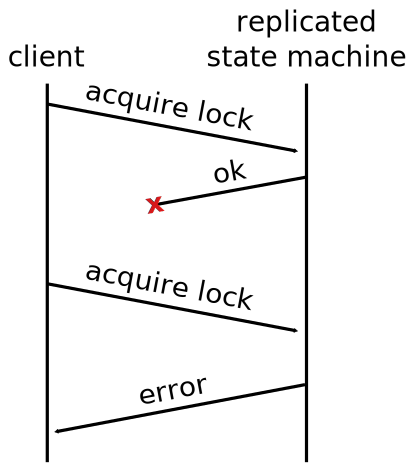
\includegraphics[scale=0.45]{clients/retrydup}
\vcaption[example of incorrect results for duplicated command]{
An example of an incorrect results that can arise from
duplicated commands. A client submits a command to a replicated state
machine to acquire a lock. The client's first command acquires the lock,
but the client never receives the acknowledgment. When the client
retries the request, it finds that the lock is already taken.
}
\label{fig:clients:retrydup}
\end{figure}

As described so far, Raft provides at-least-once semantics for clients;
the replicated state machine may apply a command multiple times. For
example, suppose a client submits a command to a leader and the leader
appends the command to its log and commits the log entry, but then it
crashes before responding to the client. Since the client receives no
acknowledgment, it resubmits the command to the new leader, which in
turn appends the command as a new entry in its log and also commits this
new entry. Although the client intended for the command to be executed
once, it is executed twice. Commands can also be applied multiple times
even without the client's involvement if the network may duplicate the
client's requests.

This issue is not unique to Raft; it occurs in most stateful distributed
systems. However, these at-least-once semantics are particularly
unsuitable for a consensus-based system, where clients typically need
stronger guarantees. Problems from duplicated commands can manifest in
subtle ways that are difficult for clients to recover from. These
problems cause either incorrect results, incorrect states, or both.
Figure~\ref{fig:clients:retrydup} shows an example of an incorrect
result: a state machine is providing a lock, and
a client finds it is unable to acquire the lock because its
original request---for which it received no acknowledgment---has
already acquired the lock. An example of an incorrect state would be an
increment operation, where the client intends for a value to increment
by one but it instead increments by two or more. Network-level
reordering and concurrent clients can lead to even more surprising
results.

Our goal in Raft is to implement linearizable semantics~\cite{Herlihy:1990}, which avoid
these classes of problems. In linearizability, each operation appears to
execute instantaneously, exactly once, at some point between its
invocation and its response. This is a strong form of consistency that
is simple for clients to reason about, and it disallows commands being
processed multiple times.

To achieve linearizability in Raft, servers must filter out duplicate
requests. The basic idea is that servers save the results of
client operations and use them to skip executing the same request
multiple times.
To implement this, each client is given a unique
identifier, and clients assign unique serial numbers to every command.
Each server's state machine maintains a \emph{session} for each client.
The session tracks the latest serial number processed for the
client, along with the associated response. If a server receives a command
whose serial number has already been executed, it responds immediately
without re-executing the request.

Given this filtering of duplicate requests, Raft
provides linearizability. The Raft log provides a serial order in which
commands are applied on every server. Commands take effect
instantaneously and exactly once according to their first appearance in
the Raft log, since any subsequent appearances are filtered out by the
state machines as described above.

This approach also generalizes to allow concurrent requests from a
single client. Instead of the client's session tracking just the
client's latest sequence number and response, it includes a set of
sequence number and response pairs. With each request, the client
includes the lowest sequence number for which it has not yet received a
response, and the state machine then discards all responses for lower
sequence numbers.



Unfortunately, sessions cannot be kept forever, as space is
limited. The servers must eventually decide to expire a client's
session, but this creates two problems: how can servers agree on when to
expire a client's session, and how can they deal with an active client
whose session was unfortunately expired too soon?

Servers must agree on when to expire a client's session; otherwise,
servers' state machines could diverge from each other. For example,
suppose one server expired the session for a particular client, then
re-applied many of that client's duplicated commands; meanwhile, the
other servers kept the session alive and did not apply the duplicates.
The replicated state machine would become inconsistent. To avoid such
problems,
session expiry must be deterministic, just as normal state machine
operations must be. One option is to set an upper bound on the number
of sessions and remove entries using an LRU (least recently used)
policy. Another option is to expire sessions based on an agreed upon
time source. In LogCabin, the leader augments each command that it
appends to the Raft log with its current time. Servers reach
agreement on this time as part of committing the log entry; then, the
state machines deterministically use this time input to expire inactive
sessions. Live clients issue keep-alive requests during
periods of inactivity,
which are also augmented with the leader's timestamp and committed to
the Raft log, in order to maintain their sessions.

The second issue is how to deal with a client that continues to operate
after its session was expired. We expect this to be an exceptional
situation; there is always some risk of it, however, since there is
generally no way to know when clients have exited. One option would be
to allocate a new session for a client any time there is no record of
it, but this would risk duplicate execution of commands that were
executed before the client's previous session was expired.
To provide stricter guarantees,
servers need to distinguish a new client from a client whose session was
expired. When a client first starts up, it can register itself with
the cluster using the RegisterClient RPC. This
allocates the new client's session and returns the client its
identifier, which the client includes with all subsequent commands. If a
state machine encounters a command with no record of the session, it
does not process the command and instead returns an error to the client.
LogCabin currently crashes the client in this case (most clients
probably wouldn't handle session expiration errors gracefully and
correctly, but systems must typically already handle clients crashing).

\section{Processing read-only queries more efficiently}
\label{clients:readonly}

Read-only client commands only query the replicated state machine; they
do not change it. Thus, it is natural to ask whether these queries can
bypass the Raft log, whose purpose is to replicate changes to the
servers' state machines in the same order. Bypassing the log offers an
attractive performance advantage: read-only queries are common in many
applications, and the synchronous disk writes needed to append entries
to the log are time-consuming.

However, without additional precautions, bypassing the log could lead to
stale results for read-only queries.
For example, a leader might be partitioned from the rest of the
cluster, and the rest of the cluster might have elected a new leader and
committed new entries to the Raft log. If the partitioned leader
responded to a read-only query without consulting the other servers,
it would return stale results, which are not linearizable.
Linearizability requires the results of a read to reflect a state of the
system sometime after the read was initiated; each read must at least
return the results of the latest committed write.
(A system that allowed stale reads would only provide
serializability, which is a weaker form of consistency.)
Problems due to stale reads have already been discovered in two
third-party Raft implementations~\cite{Kingsbury:etcdconsul},
so this issue deserves careful attention.

Fortunately, it is possible to bypass the Raft log for read-only queries
and still preserve linearizability. To do so, the leader takes the
following steps:
%
%
\begin{enumerate}
%
\item If the leader has not yet marked an entry from its current term
committed, it waits until it has done so. The Leader Completeness
Property guarantees that a leader has all committed entries, but at the
start of its term, it may not know which those are. To find out, it
needs to commit an entry from its term. Raft handles this by having each
leader commit a blank \emph{no-op} entry into the log at the start of
its term. As soon as this no-op entry is committed, the leader's commit
index will be at least as large as any other servers' during its term.
%
\item The leader saves its current commit index in a local
variable
\emph{readIndex}. This will be used as a lower bound for the version
of the state that the query operates against.
%
\item The leader needs to make sure it hasn't been 
superseded by a newer leader of which it is unaware.
It issues a
new round of heartbeats and waits for their acknowledgments from a
majority of the cluster. Once these acknowledgments are received, the
leader knows that there could not have existed a leader for a greater
term at the moment it sent the heartbeats. Thus, the readIndex was, at
the time, the largest commit index ever seen by any server in the
cluster.
%
\item The leader waits for its state machine to advance at least as far
as the readIndex; this is current enough to satisfy
linearizability.
%
\item Finally, the leader issues the query against its state machine and
replies to the client with the results.
%
\end{enumerate}

This approach is more efficient than committing read-only queries as new
entries in the log, since it avoids synchronous disk writes. To improve
efficiency further, the leader can amortize the cost of confirming its
leadership: it can use a single round of heartbeats for any number of
read-only queries that it has accumulated.

Followers could also help offload the processing of read-only queries.
This would improve the system's read throughput, and it would also
divert load away from the leader, allowing the leader to process more
read-write requests. However, these reads would also run the risk of
returning stale data without additional precautions. For example, a
partitioned follower might not receive any new log entries from the
leader for long periods of time, or even if a follower received a
heartbeat from a leader, that leader might itself be deposed and not yet
know it. To serve reads safely, the follower could issue a request to
the leader that just asked for a current readIndex (the leader would
execute steps 1--3 above); the follower could then execute steps 4 and 5
on its own state machine for any number of accumulated read-only
queries.

LogCabin implements the above algorithm on leaders, and it amortizes the
cost of the heartbeats across multiple read-only queries under high
load. Followers in LogCabin do not currently serve read-only requests.

\subsection{Using clocks to reduce messaging for read-only queries}



Up until now, the approach to read-only queries presented has provided
linearizability in an asynchronous model (where clocks, processors, and
messages can all operate at arbitrary speeds). This level of safety
requires communication to achieve: it requires a round of heartbeats to
half the cluster for each batch of read-only queries, which adds
latency to the queries.
The remainder of this section explores an alternative in which read-only
queries would avoid sending messages altogether by relying on clocks.
LogCabin does not currently implement this alternative, and we do not
recommend using it unless necessary to meet performance requirements.

\begin{figure}
\centering
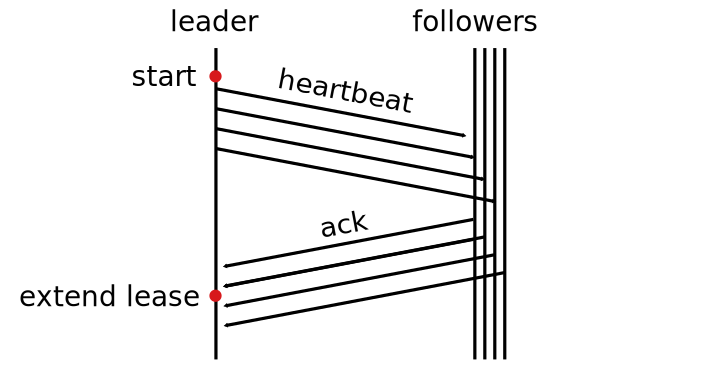
\includegraphics[scale=0.45]{clients/leases}
\vcaption[lease mechanism for read-only queries]{
To use clocks instead of messages for read-only queries,
the leader would use the normal heartbeat mechanism to maintain a lease.
Once the leader's heartbeats were acknowledged by a majority of the
cluster, it would extends its lease to $\textit{start} + \dfrac{\textit{election
timeout}}{\textit{clock drift bound}}$, since the followers
shouldn't time out before then.
While the leader held its lease, it would service read-only queries
without communication.
}
\label{fig:clients:leases}
\end{figure}

To use clocks instead of messages for read-only queries,
the normal heartbeat mechanism
would provide a form of lease~\cite{Gray:1989}.
Once the
leader's heartbeats were acknowledged by a majority of the cluster, the
leader would assume that no other server will become leader for about an
election timeout, and it could extend its lease accordingly (see
Figure~\ref{fig:clients:leases}). The leader would then reply to
read-only queries during that period without any additional
communication. (The leadership transfer mechanism presented in
Chapter~\ref{basicraft} allows the leader to be replaced early; a leader
would need to expire its lease before transferring leadership.)

The lease approach assumes a bound on clock drift across servers (over a
given time period, no server's clock increases more than this bound
times any other). Discovering and maintaining this bound might present
operational challenges (e.g., due to scheduling and garbage collection
pauses, virtual machine migrations, or clock rate adjustments for time
synchronization). If the assumptions are violated, the system could
return arbitrarily stale information.

Fortunately, a simple extension can improve the guarantee provided to
clients, so that even under asynchronous assumptions (even if clocks
were to misbehave), each client would see the replicated
state machine progress monotonically (sequential consistency).
For example, a client would not see the state as of log index $n$, then
change to a different server and see only the state as of log index $n-1$.
To implement this guarantee, servers would include the index
corresponding to the state machine state with each reply to clients.
Clients would track the latest index corresponding to results they had
seen, and they would provide this information to servers on each
request. If a server received a request for a client that had seen an
index greater than the server's last applied log index, it would not
service the request (yet).

\section{Conclusion}

This chapter discussed several issues in how clients interact with Raft.
The issues of providing linearizability and optimizing read-only queries
are particularly subtle in terms of correctness. Unfortunately, when the
consensus literature only addresses the communication between cluster
servers, it leaves these important issues out. We think this is a
mistake. A complete system must interact with clients correctly,
or the level of consistency provided by
the core consensus algorithm will go to waste. As we've already seen in
real Raft-based systems, client interaction can be a major source of
bugs, but we hope a better understanding of these issues can help prevent
future problems.


\chapter{Raft user study}
\label{userstudy}

This is the first of four chapters that each evaluate an aspect of
Raft:
\begin{compactitem}
\item This chapter evaluates Raft's understandability,
\item Chapter~\ref{correctness} discusses Raft's correctness,
\item Chapter~\ref{leaderelection} evaluates Raft's leader election
algorithm, and
\item Chapter~\ref{performance} discusses Raft's implementations and
evaluates its performance.
\end{compactitem}


\blfootnote{This study involved human subjects. It was
approved under exempt status by the Stanford University IRB
(Institutional Review Board) as Protocol~26663.}


We designed Raft to be understandable based on our intuitions and
anecdotal evidence, but we wanted to evaluate its understandability more
objectively. Although measuring understandability is inherently
difficult, this was important to us for two reasons. First, without an
evaluation, our central claim that Raft is easy to understand would be
hard to justify. Second, one of our goals was to propose understandability
as a first-class feature in computer systems, so we also carried the
burden of proposing a way to evaluate it.

To evaluate Raft's understandability, we conducted an experimental
study. This study compared students' ability to answer quiz questions
about Raft and Paxos after learning each algorithm. Our participants
were upper-level undergraduate and graduate students at Stanford
University and the University of California, Berkeley. We recorded
video lectures of Raft and Paxos and created corresponding
quizzes.
The Raft lecture covered the basic Raft algorithm
(Chapter~\ref{basicraft}) and briefly covered the joint consensus
approach to arbitrary membership changes
(Section~\ref{membership:arbitrary});
the Paxos lecture covered enough material to create an
equivalent replicated state machine, including single-decree Paxos,
Multi-Paxos, cluster membership changes, and a few optimizations needed in
practice (such as leader election).
The lecture videos and slides are available online~\cite{study}.
The quizzes tested basic
understanding of the algorithms and also required students to reason
about corner cases. Each student watched one video, took the
corresponding quiz, watched the second video, and took the second quiz.
About half of the participants did the Paxos portion first and the other
half did the Raft portion first, in order to account for both individual
differences in performance and experience gained from the first portion
of the study. We compared participants' scores on the two quizzes to determine
whether participants showed a better understanding of Raft than Paxos.

On average, participants scored 22.6\% higher on the Raft
quiz than on the
Paxos quiz (out of a possible \SI{60}{points}, the mean Raft score was 25.7
and the mean Paxos score was 21.0). Accounting for whether people learn
Paxos or Raft first, a linear regression
model predicts scores \SI{12.5}{points} higher
on the Raft quiz than on the
Paxos quiz for students with no prior Paxos experience.
Section~\ref{userstudy:results:quizzes} analyzes the quiz
results in detail.

We also surveyed participants after their quizzes to see which algorithm
they felt would be easier to implement or explain. An overwhelming
majority of participants reported Raft would be easier to implement and
explain (33 of 41 for each question). However, these self-reported
feelings may be less reliable than participants' quiz scores.
Section~\ref{userstudy:results:survey} analyzes the survey results in
detail.

Our study was unconventional for systems research, and we learned many
lessons while designing and conducting it.
For example, in a user study, almost all of the work must be done before
seeing any results; this leaves little room for error.
Two sections discuss the lessons we learned.
Section~\ref{userstudy:methodsdiscussion} explores the numerous design
decisions we considered in developing our methods and materials.
Section~\ref{userstudy:approachdiscussion} explores how effectively the
experiment convinced others of Raft's understandability, and
whether it was worth the time and effort we put into it.

\section{Study questions and hypotheses}

Our primary goal in the study was to show Raft's understandability. A
developer should be able to learn the Raft algorithm well enough to
produce a correct implementation, without an
unnecessary burden of time and effort. Unfortunately, Raft's
understandability is difficult to measure directly. There is no
established measure for understandability, and we have no way of telling
whether Raft is the most understandable possible algorithm.

To arrive at an experiment, we needed to formulate metrics that we could
measure and hypotheses that we could test.
We first needed a proxy
for measuring someone's understandability. We chose to quiz participants
and measure their quiz scores
(Section~\ref{userstudy:methodsdiscussion:testing} discusses an
alternative of having participants implement the algorithms instead).
Second, we needed to draw a comparison between participants' quiz scores
on Raft and on other consensus algorithms. We chose to compare Raft to
Paxos, the most popular consensus algorithm used today.

We wanted to explore the following questions in our study:
\begin{enumerate}

\item Is Raft easier to understand than Paxos?

We predicted students would score higher on the Raft quiz than on the
Paxos quiz.

\item Which aspects of Raft are hardest to understand?

We were interested in this question as it could help lead to further
improvements in Raft's understandability.
We thought students were most likely to struggle with commitment and
membership changes in Raft. We felt these were the most complex and
difficult aspects of Raft to explain, so students were most likely to
have difficulty understanding them
(this predates Raft's simpler single-server membership change
algorithm). We also felt that Paxos'
$\alpha$-based membership approach was simpler to explain (though the
secondary issues it leaves unsolved are significant).

\item How does knowing Paxos affect learning Raft, and vice versa?

We predicted that students would generally score higher on their second
quiz. We had two reasons for this. First, consensus algorithms share
fundamental concepts, and students should be able to grasp a concept
more easily when seeing it a second time. Second, since the lectures and
quizzes followed the same format, we thought students would gain useful
experience during the first lecture and quiz.

\item Do people prefer to use Raft over alternatives?

We predicted Raft's understandability would result in a preference to
implement and explain Raft.

\end{enumerate}


\section{Discussion about the methods}
\label{userstudy:methodsdiscussion}

%

Because there is little precedent for this sort of experiment in
computer systems literature, we reasoned through many our experimental
design decisions from first principles.
We are especially thankful for Scott Klemmer's valuable help during this
process.
This section explains why we arrived at our methods by
describing the alternatives we considered for each decision,
including:
\begin{compactitem}
\item Our
choice of participants and how to motivate their participation
(Section~\ref{userstudy:methodsdiscussion:participants}),
\item
How to teach the algorithms to the participants
(Section~\ref{userstudy:methodsdiscussion:teaching}),
\item
How to test their understanding
(Section~\ref{userstudy:methodsdiscussion:testing}),
\item
How to evaluate their performance
(Section~\ref{userstudy:methodsdiscussion:grading}),
\item
What questions to ask in the survey
(Section~\ref{userstudy:methodsdiscussion:survey}),
and
\item
How to discover and fix problems in the study before starting
(Section~\ref{userstudy:methodsdiscussion:pilots}).
\end{compactitem}
The methods we ultimately decided to use are then presented in
Section~\ref{userstudy:methods} in a more formal APA
(American Psychological Association) style.

One common principle we applied was to test participants at the start
of the learning curve for the algorithms. We wanted to see how easily
they could move from no knowledge to a moderate level of understanding.
While we hoped that our participants would gain at least a basic
understanding of both algorithms, we did not
want to over-prepare them. Given infinite time, most participants will
eventually understand any consensus algorithm. Thus, to measure a
difference between algorithms, we had to test participants at the
start of the learning curve. For example, this meant we faced a tension
in motivating participants, as discussed in the next subsection: we
wanted them to try, but we did not want them to study the algorithms
extensively.

\subsection{Participants}
\label{userstudy:methodsdiscussion:participants}

We invited students from both Stanford and Berkeley to participate in our
study. This both
increased our sample size and broadened the generality of our results. We
chose to use the same materials and procedures in both schools so that
we could compare participants' performance across schools.

We considered various ways to use course grades to incentivize students
to participate in the study. We wanted students to put equal effort into
learning each algorithm, and we only wanted them to watch the lectures
to prepare (without using outside information or studying excessively).
Unfortunately, we had substantial
concerns for each approach we considered to incentivize students:
\begin{itemize}
\item If students' participation affected their course grades but they
earned credit for even incorrect answers, we were concerned that
students might not pay attention to the lectures. For example, a student
who skipped the lectures but filled in the quizzes with any answer that
came to mind would still receive full credit towards his/her course grade.
\item If students' scores on their quizzes affected their course grades,
we were concerned that students might spend too much time preparing for
the quizzes or that they might work harder on the more difficult to
understand algorithm in
order to earn the same grade. We wanted to test participants at the
start of the learning curve; we didn't want students to understand the
algorithms so well that our questions could measure no difference in
understanding between the algorithms. We also wanted them to spend equal
effort on each algorithm.
\item If students were awarded extra course credit for participation or
for good quiz scores, we were concerned that poorly performing or more
stressed students might be overrepresented in our participants.
\item Another idea we considered was to award students all of the course credit 
for scoring at least 50\% on \emph{either} quiz. Our
concern with
this approach was that it would leave too many possible explanations for
quiz scores. For example, would students stop after their first
algorithm if they believed they did well enough? Would students choose
ahead of time to try to do well on Raft and not worry about the Paxos
quiz (or vice versa)?
\end{itemize}

For the Stanford students, we ultimately decided to give full course
credit (5\% of the total course grade)
for reasonable participation in the study. We intentionally left
this definition vague, but if a student appeared to put some effort into
the study, we awarded them full course credit. The students were also
informed that the material might show up again on the course's final
exam. Almost every student in the Stanford class participated (see
Table~\ref{tab:userstudy:participation}).

However, the only incentive for the Berkeley participants was the
opportunity to learn the material.
The instructors for the Berkeley class chose not to factor study
participation into the course grades, and the class did not have exams.
Even without additional incentives, at least one third of the students
in the Berkeley class
participated (see Table~\ref{tab:userstudy:participation}).

\begin{table}
\centering
\begin{tabular}{lrrrrc}
school & total & \ $\geq$ one quiz & \ $\geq$ both quizzes & full study
& incentive \\
\hline
\noalign{\vskip .75ex}
Stanford & 34 & 33 & 31 & 31 & 5\% part.\ grade, final exam \\
Berkeley & 46 & 16 & 12 & 11 & none \\
Total    & 80 & 49 & 43 & 42 & - \\
\end{tabular}
\vcaption[study participation]{
Study participation.
The ``total'' column lists the number of students in each class;
the ``$\geq$ one quiz'' column lists the number that completed at least
one quiz;
the ``$\geq$ both quizzes'' column lists the number that completed at least
both quizzes;
and
the ``full study'' column lists the number that completed
both quizzes and the survey.
\\
The total number of participants is approximate. For Berkeley, this
number is based on the course email list and is likely an over-estimate
(only 25 students signed up to do the homework towards the end of the
course).
}
\label{tab:userstudy:participation}
\end{table}

\subsection{Teaching}
\label{userstudy:methodsdiscussion:teaching}

We had many options in how to teach the algorithms to the participants.
Not only are there many ways to teach in general, but there are also
various approaches to teaching Paxos in particular. Our goal in the
study was to compare the algorithms, not the ways they were conveyed.
Therefore, it was important for the teaching method and style to be
consistent. We wanted to convey the algorithms in similar ways, and we
wanted to cover equivalent content.
We also wanted participants to spend no more than a few hours per
algorithm. We thought this would be reasonable to ask of our
participants, and we would then be able to test them at the start of the
learning curve for each algorithm.

We considered using papers to teach our participants, but this had two
problems.
First, we could not find a suitable Paxos paper. This paper would have
had to:
\begin{compactitem}
\item Cover a relatively understandable variant of Paxos (there is no
single agreed upon Paxos algorithm, but some are easier to understand
than others);
\item Describe it completely enough to build a replicated state
machine;
\item Be accessible to students with no background in the topic,
without needing to understand related work first; and
\item Be of similar quality, style, and length to the Raft paper.
\end{compactitem}
We could have written such a paper, but it would have taken months.
The second problem is that papers take many hours to read,
and we wanted the participants to be able to learn
the algorithms in less time.

Instead, we decided to teach the participants through lectures. We
estimated that we could cover enough material for each algorithm in a
one-hour lecture. This was short enough that it didn't unduly burden
our participants, yet it was long enough to cover a significant amount of
material at a comfortable pace. It was also short enough that we
could still quiz participants towards the start of the learning curve
for the algorithms.

We chose to have John Ousterhout give the lectures for both algorithms,
rather than using a different lecturer for Paxos. In trying to maximize
consistency across the algorithms, we considered the following factors
in our decision:
\begin{itemize}
\item \textbf{Expertise:} We wanted an equivalent level of expertise on
each algorithm, and we didn't consider ourselves experts on Paxos before
the study. We could have brought in an expert on Paxos to give the Paxos
lecture. Instead, Ousterhout based his slides on those of experts, and
in preparing for the Paxos lecture, we believe we learned Paxos well
enough to consider ourselves sufficiently knowledgeable in it.
\item \textbf{Teaching style and ability:} Ousterhout was able to keep
this very consistent across his two lectures, whereas we might have
struggled with different teaching styles and abilities if a separate
lecturer gave the Paxos lecture.
\item \textbf{Lecture quality:} Ousterhout giving both lectures raises
concerns that he might not have put in the effort to produce an equally
good Paxos lecture. However, he tried to produce equivalent lectures,
and this is mitigated by basing his Paxos slides off of those of
experts. (Also, the Raft lecture had known deficiencies during the
study: we made some last-minute changes to fix a bug in it that could
have been clearer if we had more time. Moreover, it presented the more
complex form of membership changes, as it predated the simpler
single-server change algorithm.)
Balancing lecture quality might
have been more difficult with a different Paxos lecturer, since the
second lecturer may not have been as committed to the study.
\end{itemize}


We wanted to teach a variant of Paxos that was relatively
understandable and complete, while staying true to the fundamentals of Paxos.
Unfortunately, there is no agreed upon variant of Paxos; different
instructors disagree on which variant to teach.
We ultimately settled on a variant from David Mazi\`eres~\cite{dmpaxos},
which is not only efficient but also relatively understandable.
However, we used Leslie Lamport's $\alpha$ approach~\cite{Lamport:2001} to
reconfiguration rather than Mazi\`eres's. Although Lamport's approach has the
undesirable property that it limits Paxos's concurrency during normal
operation, we (including Mazi\`eres) believe its basic idea is easier to
understand than Mazi\`eres's and other approaches.

We recorded both lectures on video rather than having John Ousterhout
present them in person. There were several advantages to recording them:
\begin{compactitem}
\item We could fit more material in the same amount of time, since we
could re-record segments when we made mistakes.
\item We were able to debug problems with our lectures during the two
pilot studies we ran for each algorithm
(see Section~\ref{userstudy:methodsdiscussion:pilots}).
Having them recorded allowed us to catch issues and fix them reliably.
\item Participants could watch the lectures in different orders and
still see the same exact material.
\item Students could watch the lectures at their own pace and at their
own schedule. They could re-watch segments or speed up and slow down the
videos as they wished. We did not enforce time limits on the lectures,
so students could watch them at their own pace.
\item The video lectures remain as documentation for the study and could
be used in a repeated study. Other people outside the study have also
used the videos to learn the algorithms on their own
(our Raft lecture has \num{14480} views on YouTube as of August 2014,
and our Paxos lecture has \num{9200} views).
\end{compactitem}
A possible disadvantage is that students could not ask questions during
the lectures. On the other hand, questions would have disrupted the
consistency benefits of having recorded lectures. For example, questions
could lead to more material being presented in one lecture than another
and could introduce additional differences between the Stanford and
Berkeley groups. We also do not know
how the recorded lectures affected study participation; while our
Stanford participation was high, it's possible that
we could have gotten higher participation at Berkeley by scheduling the
lectures in class.

We attempted to keep the video lectures fairly impersonal to reduce
bias. For example, the video components only showed the lecture slides
and not John Ousterhout himself. However, even Ousterhout's voice-over may
have been subtly biased (though he tried not to be). Concerned readers
should review the lecture videos to decide for themselves; we do not
know of any formal techniques to measure or reduce such bias.

In addition to the video lectures, we provided participants with minor
additional materials for their preparation (lecture notes and algorithm
summaries). We discouraged participants from learning about the
algorithms on their own (for example, by reading papers), but we felt
that some additional materials to review before the quiz and to reference
during the quiz would be helpful for the participants. We made copies of
the lecture slides available for easier reference, and we provided
participants with algorithm summaries in the form of a (condensed)
one-page summary for Raft and a (sparse) 3.5-page summary for Paxos.
These are included in Appendix~\ref{appendix:userstudy:supporting}.


\subsection{Testing understanding}
\label{userstudy:methodsdiscussion:testing}

A key challenge of this study was how to measure participants'
understanding of the algorithms.
%
We considered having participants implement the algorithms, which would
allow us to measure their ability to build working systems more
directly. If feasible, this approach would have been better than the
quizzes. However, we chose not to do
this because of numerous challenges. First, we estimate that implementing
significant portions of Raft or Paxos would take most experts weeks. If
we asked this of our participants, surely we would not have had so many,
and we might not have been able to draw statistically significant
conclusions. Moreover, peoples' ability to develop systems varies
greatly, so to draw statistically significant conclusions, such a study
would need large sample sizes or would need each participant to
implement both algorithms. Both options would be difficult in practice
because of the time commitment required of participants. Even if the
participation problems were solved, it would still be challenging to
measure implementations against each other. A thorough treatment would
need to include metrics of correctness, code complexity, and cost, all
of which are challenging to measure.

Instead, we chose to quiz participants to measure their understanding.
This required less time of our participants. As a result, we were able
to have each participant learn both algorithms, which
made it easier to factor out individual differences in learning and
test-taking abilities. Moreover, it was easy to compare
participants' performance based on their numeric quiz scores.

Our most difficult challenge in developing the quizzes was how to make
them fair. We first considered using questions that
applied equally to both algorithms, but such questions tended to be
too obvious for one of the algorithms because it more directly covered
the topic. Instead, we only used similar questions if the
difficulty would also be similar.

We used the following strategy to make the quizzes fair. First, we
categorized each question by difficulty:
\begin{compactitem}
\item Easy questions were essentially recall: the answer could be found in the
lecture with little or no inference. We expected students to
answer nearly all of these correctly.
\item Medium questions required the participant to apply an algorithm found in
the lecture, but it should have been straightforward to determine which
steps to apply.
\item Hard questions required the participant to figure out what rules to
apply, combine them in new ways, and/or extrapolate beyond the lecture
material. We expected that few students would be able to
answer these questions perfectly.
\end{compactitem}
Questions in the same difficulty category should require about the same
amount of inference and extrapolation from the lecture material.
We (re-)categorized questions after the lectures were created in order
to ease concerns of ``teaching to the quiz''.

Second, we assigned point values to each question based on how long we expected
it to take. The point values were intended to reflect how many minutes
it would take a reasonably prepared student to answer the question,
based on John Ousterhout's teaching experience. For example, a question that was
expected to take about five minutes was worth five points.

Third, we balanced the quizzes in categories and points. Each quiz
contained \SI{4}{points} of easy questions,
\SI{26}{points} of medium questions, and
\SI{30}{points} of hard questions.
We also compared the questions from each
quiz side-by-side to confirm that they seemed equally difficult.

We believe the quizzes we produced this way are similar in
difficulty, though we have no way to know for sure. We ask readers to
decide for themselves by reviewing the quizzes found in
Appendix~\ref{appendix:userstudy}.

Most of the questions required open-ended short answers. We also
considered using multiple choice questions, which would have been easier
to grade objectively. However, we decided on the open-ended format
because we feel it more effectively tests participants' understanding,
as it is less suggestive of responses.

The quizzes were limited in time so that participants were unable to
become experts on the questions. We did not want to give them enough
time to attempt the questions, watch the entire video again, and then
revise the answers.

In order to extract the most information from the quizzes, we made them
intentionally difficult. For example, we didn't want any participants to
earn a perfect score because then we wouldn't have been able to
distinguish differences between them. However, we later determined that
we made the quizzes a bit too hard: the maximum score was only 46.5 out
of 60. For example, most students earned 0 points on question 8 on
each quiz; had we made those questions easier, we might have been able
to better distinguish the differences between those students.

\subsection{Grading}
\label{userstudy:methodsdiscussion:grading}

We graded the quizzes using two passes. The initial (preliminary)
grading pass was more subjective, assigning grades based on perceived
understanding. The second (final) pass assigned
grades more objectively. The following steps summarize our
procedure:
\begin{compactenum}
\item Diego Ongaro and John Ousterhout created a plausible rubric.
\item Ongaro graded the quizzes fairly quickly (grading all participants
for a given question at a time in random order, alternating between
Paxos and Raft between each question).
\item Ongaro and Ousterhout revised the rubric based on problems that
arose.
\item Ongaro regraded the quizzes more carefully (grading all
participants for a given question at a time in order of
their preliminary scores, alternating between Paxos and
Raft between each question).
\end{compactenum}
The final grading rubrics are included in Appendix~\ref{appendix:userstudy}
along with the quiz questions.

We awarded partial credit in order to gain the most information from the
quiz scores as possible. For example, a blank response demonstrates no
understanding, whereas one that is on track to an answer demonstrates
some understanding; we wanted to distinguish these cases. We tried to
award points proportional to the understanding that the participant
demonstrated in his/her answer.

There are two things we could have done better. First, we exposed
ourselves to preliminary scores and results prior to completing the rubric and
adjusting the grading. It
would have been safer to avoid this, since it raises concerns that we
might have, for example, awarded fewer points to Paxos answers during the
second round of grading if we thought it was going to be a close call.
Although we question this aspect of our procedure, it is not too
worrisome because the grades and overall results and conclusions
were essentially the same after the second pass of grading. 
For example, the Raft mean was 25.74 after the preliminary pass of
grading and 25.72 after the final pass; the Paxos mean was
20.77 after the preliminary pass, then corrected to 20.98.

Second, we graded the quizzes ourselves, and this may have introduced
bias, since we hoped that the study would show that Raft is easier to
understand than Paxos. We graded ourselves because it
takes expertise in the algorithms to develop rubrics and grade responses
(which sometimes vary greatly from each other). Therefore, it was
easiest for us to do these tasks ourselves. However, we could have hired
impartial graders to confirm our grading using our rubric.


\subsection{Survey}
\label{userstudy:methodsdiscussion:survey}

We initially considered asking participants whether they understood Raft
better than Paxos, rather than quizzing them. We were informed that such
a survey would not be very reliable on its own. For example,
participants might respond favorably towards Raft if they believe that
is our desired outcome (\emph{social desirability bias}), or they may be affected by
wording in the questions. Although we settled on quizzes
for our primary results, there is still some value in
asking participants for their opinions, so we included a short survey
for participants to fill out after their second quiz.

Our survey included six questions using five-point scales (\emph{Linkert
items}) and one open-ended question for general feedback or comments. We
tried to keep the survey short to encourage participation, and the
answers were easy to collect and quantify this way.

\subsection{Pilots}
\label{userstudy:methodsdiscussion:pilots}

One challenge with this type of study is that it is very costly if
things go wrong and the study needs to be repeated. To mitigate this
risk, we attempted to discover and iron out problems with our materials
and procedures before launching the study. Thus, we conducted two pilot
studies, each with two to four volunteer participants who were not part
of the normal study.
We included \SI{90}{points} of questions on each of
the pilot quizzes; that way we could try more questions than we intended
to keep and would have the option to throw out bad questions
(our pilot quizzes included more easy questions than the final quizzes,
but we cut most of them to shorten the quizzes).
We corrected many
problems with the lectures and quizzes during the pilots, and we
feel that the pilot process was essential to the study's success.

\section{Methods}
\label{userstudy:methods}

This section describes the methods of the Raft user study in a more
formal APA
(American Psychological Association) style. It includes many technical
details that are less conceptual in nature than the topics discussed in
Section~\ref{userstudy:methodsdiscussion} but are nevertheless important
to the study.

\subsection{Study design}

The experiment employed a \emph{within-subjects} design in which each
participant was quizzed on both the Paxos and the Raft algorithms. To
account for ordering effects, it was also \emph{counterbalanced}: about
half of the participants learned Paxos and took the Paxos quiz, then
learned Raft and took the Raft quiz; the other half learned Raft and
took the Raft quiz, then learned Paxos and took the Paxos quiz.

There were two key independent variables:
\begin{compactitem}
\setlength{\itemindent}{2em}
\item Which algorithm (Paxos or Raft)?
\item Which order (Paxos then Raft, or Raft then Paxos)?
\end{compactitem}

We recorded two additional independent variables, though we hoped their
effects would be minor:
\begin{compactitem}
\setlength{\itemindent}{2em}
\item Which school did the participant come from (Stanford or Berkeley)?
\item Did the participant have prior experience with Paxos?
\end{compactitem}


\subsection{Participants}

We invited students from Stanford and Berkeley to participate in our
study. Table~\ref{tab:userstudy:participation} summarizes the
participation from each group and how many participants completed each
portion of the study.

The 33 Stanford participants were recruited from the Advanced
Operating Systems (CS240) course at Stanford University offered January
through March 2013 and taught by David Mazi\`{e}res. The students were
upper-level undergraduate and graduate students, and a small
number of remote professional students (SCPD). They were informed that
``reasonable participation'' in the study would award them
5\% of their
course grade. (They were also offered an alternate option should they
choose not to participate in the study.) They were also informed that
questions on the material may reappear on the final exam for the course.

The 16 Berkeley participants were recruited from the Distributed
Computing (CS294-91) course at the University of California, Berkeley
offered January though May 2013 and taught by Ali Ghodsi. The students
were mostly graduate-level (though at least one undergraduate student
took the course). It was vaguely suggested to the students that they
should participate in the study as part of the course, but there was no
explicit incentive to encourage participation.

\subsection{Materials}

Participants gained access to materials for the study though a
password-protected website.
The website allowed participants to proceed with the study at their own
pace and at any time of day. The various materials available on the
website are explained in more detail next.

\subsubsection{Lectures}

\begin{figure}
\centering
\fbox{
\includegraphics[scale=.5]{userstudy/stylusoverlay}
}
\vcaption[example lecture slide with stylus overlay]{
Example lecture slide marked up with stylus overlay. This slide comes
from the Paxos lecture (it shows liveness problems that could arise if
two competing proposers were too synchronized).
}
\label{fig:userstudy:stylusoverlay}
\end{figure}

Each algorithm had a corresponding video lecture. The lecture slides
were designed and created by John Ousterhout. The Paxos lecture
borrowed from slides by Lorenzo Alvisi, Ali Ghodsi, and David
Mazi\`{e}res; the Raft lecture was based on a draft of a paper
describing Raft.
The slides were made available
to the participants on the study website in both Microsoft PowerPoint
and PDF formats. The videos used a ``screencast'' format: the video
components showed only the slides and a stylus overlay, and the audio
component consisted of Ousterhout verbally explaining the slides.
Figure~\ref{fig:userstudy:stylusoverlay} shows an example of a slide with the
stylus overlay.
The
videos were recorded in advance so that students in both ordering groups
could use the same exact videos. They were made available to the
students on both the YouTube video hosting website and in MP4
format for download.

The Raft lecture covered the following topics: leader election, log
replication, safety, client interaction, and the joint consensus
approach to membership changes.
The Paxos lecture covered enough material to create an equivalent
replicated state machine, including single-decree Paxos,
Multi-Paxos, client interaction, membership changes, and a few
optimizations needed in practice (such as leader election).
Log compaction was not included in either
lecture.

\begin{table}
\centering
\begin{tabular}{lrlrlrl}
algorithm &
  \multicolumn{2}{c}{lecture slides} &
  \multicolumn{2}{c}{lecture duration (MM:SS)} &
  \multicolumn{2}{c}{lecture word count} \\
\hline
\noalign{\vskip .75ex}
Raft &
  \hspace{1em} \num{31} & &
  \hspace{2em} 58:18 & &
  \hspace{1em} \num{10053} & \\
Paxos &
  \num{33}    & \hspace{-1em} (+6\%) &
  66:34       & \hspace{-1em} (+14\%) &
  \num{11234} & \hspace{-1em} (+12\%) \\
\end{tabular}
\vcaption[lecture lengths]{
Various measures of length for the two lectures. The lecture word count
is an approximation based on automated YouTube transcripts of the
lecture videos. The percentages in parenthesis show the additional
length of the Paxos lecture relative to the Raft lecture.

\vspace{3ex}
}
\label{tab:userstudy:lecturelength}
\end{table}

We aimed to create video lectures that were about one hour in length. We
tried to balance the lectures so they covered the material at an
equivalent level of detail with similar numbers of examples. This
resulted in the Paxos lecture being slightly longer than the Raft
lecture. Table~\ref{tab:userstudy:lecturelength} compares their lengths using
various metrics.

\subsubsection{Supporting materials}

Both lectures included optional summaries of the algorithms.
For the Raft lecture, the summary was a single slide
(participants needed to zoom into this slide to read it).
For Paxos, a 3.5-page summary of the single-decree and Multi-Paxos algorithms
was provided along with the lecture on the study website.
These are included in Appendix~\ref{appendix:userstudy:supporting}.
Participants did not need to
view the summaries to score well on the quizzes, but they were provided
as quick reference and review materials.
We did not track whether participants actually viewed the summaries.

\subsubsection{Quizzes}
\label{userstudy:methods:materials:quizzes}

Each algorithm included a web-based quiz.
The quizzes and their solutions and grading rubrics are provided in
Appendix~\ref{appendix:userstudy}.
The quizzes tested basic understanding of the algorithms and also
required students to reason about corner cases.
Most of the questions required open-ended short answers.
Each quiz consisted of eight questions of varying difficulty (some were
multi-part questions). We categorized the questions using a difficulty
rating scale (see Section~\ref{userstudy:methodsdiscussion:testing}):
\begin{compactitem}
\item The first question (\SI{4}{points}) was rated easy.
\item The next four questions (\SI{26}{points}) were rated medium.
\item The last three questions (\SI{30}{points}) were rated hard.
\end{compactitem}
The point values were intended to reflect how many minutes it would take
a reasonably prepared student to answer the question.
Participants were given the point values, but questions on the quizzes were
not explicitly labeled with their difficulty ratings.

Unfortunately, the Paxos quiz used in the study had one typo in
Question~4. The original question used in the study and the correction
can be found in Appendix~\ref{appendix:userstudy},
along with a description of how the question was graded.

Participants were instructed to complete each quiz within
\SI{60}{minutes}.
The website included a decreasing counter with minute-level granularity
(we were advised that finer-grained counters can cause unnecessary
anxiety). No technical measures were employed to force students to
submit their answers within \SI{60}{minutes}. At the end of
\SI{60}{minutes}, this
counter would go negative. However, participants' web browsers reported
the full elapsed quiz time, and the server kept records of the time when
the participant first opened a quiz and when he/she submitted each quiz.
Only four participants
went more than 10\% over the time limit (we included those quizzes
anyway in the results presented in
Section~\ref{userstudy:results:quizzes}).


\subsubsection{Survey}

Following their second quiz, participants were asked to complete a short
web-based survey, which can be found in
Appendix~\ref{appendix:userstudy:survey}.
It consisted of six questions using five-point scales (\emph{Linkert
items}) and one open-ended question for general feedback or comments. It
included questions about their prior experience with Paxos and whether
they would prefer to implement or explain one of the algorithms over the
other.

\subsection{Dependent measures}

Participants' performance on the quizzes formed the primary dependent
measure for this study. Diego Ongaro graded the quizzes in random order
according to a rubric. Ongaro was blind as to the participants'
schools during grading (and was and still is blind as to the
participants' identities). Participants' preferences in the survey were
also a dependent measure.

\subsection{Procedure}

Participants were randomly assigned to an ordering group (Paxos first or
Raft first) over e-mail. This e-mail instructed the participants to
complete the first quiz by 11:59~p.m.\ on a Monday and the second quiz by
11:59~p.m.\ on that Friday (though we accepted both early and late
responses). The e-mail included a link to the study website and unique
login credentials for each participant.

The study website included the materials described above. Participants
could visit the website at any time. They were
not timed as they watched the videos or studied the supporting materials.
The website instructed them that they would have \SI{60}{minutes} to
complete the quiz once they opened it. The website saved the quiz
responses frequently and reloaded them in case the participant reopened
the quiz page. After submitting the second quiz, the website prompted
the participant to fill out the survey.

\section{Results}

This section presents the results obtained from our experiment.
Section~\ref{userstudy:results:quizzes} describes the quiz results, and
Section~\ref{userstudy:results:survey} describes the survey results.


%

\subsection{Quizzes}
\label{userstudy:results:quizzes}

\begin{figure}
\centering
{
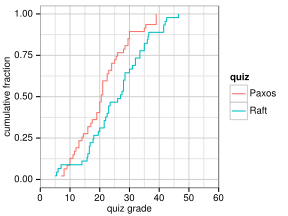
\includegraphics{userstudy/unpairedcdf}
}
\vcaption[quiz score CDF]{
CDF of participants' quiz scores.
Each curve shows the fraction of participants who scored at most
that many points (right/lower is better); for example, about 47\% of
participants scored up to 25 points on the Raft quiz; the remaining 53\%
scored higher.
The maximum possible score was \SI{60}{points} on each quiz.
47 participants completed the Paxos quiz; 45 completed the Raft quiz.
Figure~\ref{fig:userstudy:diffBreak} facets this graph down by question
difficulty and ordering.
}
\label{fig:userstudy:unpairedcdf}
\end{figure}

Figure~\ref{fig:userstudy:unpairedcdf} shows the raw distributions of quiz scores;
the Raft scores are generally greater than the Paxos scores by
a few points.
The mean Raft score is \SI{4.74}{points} or 22.6\% higher than
the mean Paxos score.
We used a statistical significance test to confirm this difference:
we conducted an unpaired Student's \emph{t}-test with a one-sided
hypothesis that the Raft scores were greater than the Paxos scores.
This test found that
the Raft scores (\emph{M}~=~25.72, \emph{SD}~=~10.33) were significantly
greater than the Paxos scores (\emph{M}~=~20.98, \emph{SD}~=~8.57);
\emph{t}(85.55)~=~2.39, \emph{p}~=~0.009.
In layman's terms, we can say with 99\%
confidence from our sample that the true distribution of Raft quiz
scores is greater than the true distribution of Paxos quiz scores
(there is only a 1\% chance that we would find such a difference by
random chance in identical distributions; a $p$-value less than 5\%
is typically considered statistically significant).

\begin{figure}
\centering
{
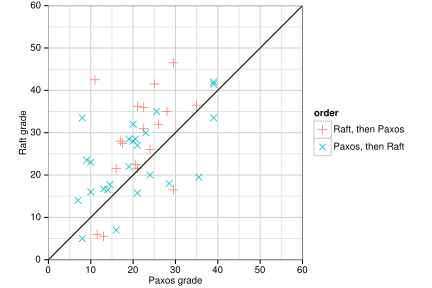
\includegraphics{userstudy/pairedscatter}
}
\vcaption[quiz score scatter plot (by school)]{
A scatter plot of 43 participants' grades comparing their performance on
each quiz. Points above the diagonal (33) represent participants who
scored higher on the Raft quiz.
The shape and color of each point represent whether that particular
participant watched the Raft lecture and took the Raft quiz first or
whether he/she watched the Paxos lecture and took the Paxos quiz first.
Figure~\ref{fig:userstudy:pairedscatterpaxos} is a similar scatter plot which
shows participants' prior Paxos exposure instead.
}
\label{fig:userstudy:pairedscatter}
\end{figure}

\begin{figure}
\centering
{
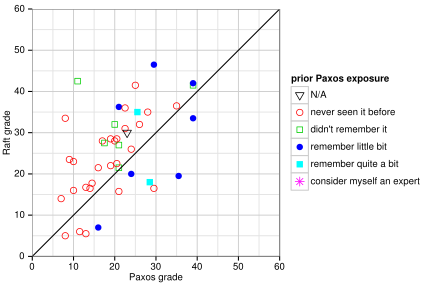
\includegraphics{userstudy/pairedscatterpaxos}
}
\vcaption[quiz score scatter plot (by prior Paxos exposure)]{
A scatter plot of 43 participants' grades comparing their performance on
each quiz, showing the participants' prior Paxos exposure.
The shape and color of each point represent the prior Paxos exposure
that participant reported in the survey
(the exact question can be found in
Appendix~\ref{appendix:userstudy:survey}). One participant did not
respond to the question (labeled ``N/A'').
No students reported prior Raft exposure.
Figure~\ref{fig:userstudy:pairedscatter} is a similar scatter plot which
shows the order in which participants took the quizzes instead.
}
\label{fig:userstudy:pairedscatterpaxos}
\end{figure}

\begin{figure}
\centering
{
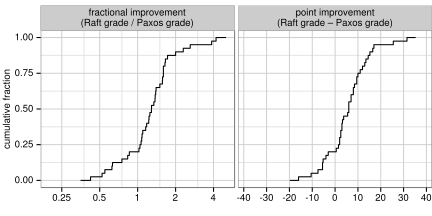
\includegraphics{userstudy/pairedcdf}
}
\vcaption[CDF of participants' quiz score difference]{
CDF of 43 participants' Raft scores compared to their Paxos scores.
The left graph shows participants' relative score difference between the
quizzes (an $x$-value of 2 means the participant's score on the Raft
quiz was twice their score on the Paxos quiz).
The right graph shows the participants' absolute score difference
between the quizzes (positive values represent participants who scored
higher on Raft).
}
\label{fig:userstudy:pairedcdf}
\end{figure}

We also wanted to consider individual differences in learning and
test-taking abilities. Because participants learned and took quizzes
on both algorithms, we could look at each participants' difference in
quiz scores. (Six participants only took one quiz, so we exclude them
here.)

Figures~\ref{fig:userstudy:pairedscatter} and \ref{fig:userstudy:pairedscatterpaxos} plot
individuals' quiz scores against each other. They show that 33 of 43 of
the participants scored higher on their Raft quiz than on their Paxos
quiz. Figure~\ref{fig:userstudy:pairedscatter} overlays the order in which
participants learned the algorithms and took the quizzes, while
Figure~\ref{fig:userstudy:pairedscatterpaxos} overlays participants' prior Paxos
exposure. Neither of these appear to be obviously correlated with which
participants scored higher on their Raft quiz.

Figure~\ref{fig:userstudy:pairedcdf} shows the overall distribution of
how participants scores differ across exams; this makes it easier to
compare the overall behavior of the data.
The participants' scored a median of \SI{6.5}{points} or
31.7\% higher on
the Raft quiz than on the Paxos quiz.
We conducted a paired samples \emph{t}-test with a one-sided
hypothesis that participants Raft scores were generally greater than
their Paxos scores.
This test found that
individuals' Raft scores (\emph{M}~=~25.73, \emph{SD}~=~10.56) were
significantly
greater than their Paxos scores (\emph{M}~=~20.79, \emph{SD}~=~8.64);
\emph{t}(42)~=~3.39, \emph{p}~=~0.001.
In layman's terms, we can say with 99.9\%
confidence from our sample that similar individuals will
score greater on their Raft quiz than on their Paxos quiz
(there is only a 0.1\%
chance that we would find such a difference by
random chance in identical distributions).

\begin{figure}
\centering
{
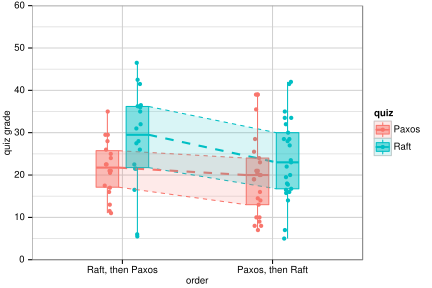
\includegraphics{userstudy/order}
}
\vcaption[ordering effects]{
Ordering effects on participants' quiz scores.

The boxplots summarize the participants' quiz score distributions. The
top of each line is the maximum score attained, the top of each box is
the $\mathrm{75}^\mathrm{th}$ percentile, the middle of each box is the
median, the bottom of each box is the $\mathrm{25}^\mathrm{th}$
percentile, and the bottom of each line is the minimum score attained.

Dashed lines connect the quantiles on boxplots for the same quiz between
different ordering groups. For example, the thick, dashed, blue line
connects the median score for the Raft quiz in the group that took the
Raft quiz first (left) to the median score for the Raft quiz in the
group that took the Raft quiz second (right). If the ordering of the
quizzes did not affect participants' performance, these dashed lines would
be nearly horizontal.

Participants' individual quiz scores overlay each boxplot to provide
further detail. Each point's \emph{x} coordinate is randomly offset to
reduce overlap.
}
\label{fig:userstudy:order}
\end{figure}

We were also curious whether the order in which students learned the systems
affected their quiz scores.
Figure~\ref{fig:userstudy:order} shows participants' quiz scores grouped by
whether they took the Raft quiz first or second.
It appears from the figure that the participants who took the Raft quiz
first scored about five points higher on the Raft quiz than those who
took the Paxos quiz first.
To investigate this effect, we used statistical tests to determine
whether the scores in the two groups truly differed for the same quiz:
we conducted
unpaired \emph{t}-tests with two-sided hypotheses that the groups
differed in either direction.
These showed no statistically significant differences between
the groups; such a difference for Raft could occur by random
chance in 16.8\% of similar experiments.
However, ordering does appear to be a statistically significant factor
when also considering prior Paxos experience; this is discussed next as
a component of a linear regression model.

We created a linear regression model to investigate the effects of various factors
on quiz scores. The model considered whether the participants were
taking their first or second quiz, their prior Paxos experience, and
their school. To test whether ordering and prior Paxos experience
affected the Raft or Paxos quizzes differently, the linear model
included two variables for each of those. Thus, the model included the
following variables:
\begin{compactitem}
\item \textbf{Quiz:} Paxos or Raft.
\item \textbf{Second quiz, Raft:} the participant took the Paxos quiz before
the Raft quiz, and \emph{Quiz} is Raft.
\item \textbf{Second quiz, Paxos:} the participant took the Raft quiz before
the Paxos quiz, and \emph{Quiz} is Paxos.
\item \textbf{Prior Paxos experience, Raft:}
the participant's prior Paxos experience if the \emph{Quiz} is Raft,
0 otherwise. In order to include this factor in the model,
participants' prior Paxos experience was mapped from the
English answer labels found in Appendix~\ref{appendix:userstudy:survey}
to integers between 0 and 4.
\item \textbf{Prior Paxos experience, Paxos:}
the participant's prior Paxos experience if the \emph{Quiz} is Paxos,
0 otherwise.
\item \textbf{School:} Stanford or Berkeley.
\end{compactitem}

Our first model (Table~\ref{tab:userstudy:lm1}) reported that the \emph{School}
factor was insignificant, so we created a second model that excludes it.
The second model, shown in Table~\ref{tab:userstudy:lm2}, explains
19\% of the
variance in quiz scores; the other 81\% at least includes individual
differences in learning and test-taking abilities. Accounting for
ordering, this model predicts quiz scores
that are \SI{12.5}{points} higher on the Raft quiz than on the Paxos quiz for
students with no prior Paxos experience.

\begin{table}
\centering
\begin{tabular}{lrrrr}
variable & estimate & std. error & \emph{t}-value & \emph{p}-value \\
\hline
\noalign{\vskip .75ex}
Intercept                       & $10.61$ & $3.32$ &  $3.19$ & $0.002$ \\
Quiz is Raft                    & $12.99$ & $4.46$ &  $2.92$ & $0.005$ \\
Second quiz, Raft               & $-6.74$ & $2.87$ & $-2.35$ & $0.021$ \\
Second quiz, Paxos              &  $4.09$ & $2.87$ &  $1.42$ & $0.158$ \\
Prior Paxos experience, Paxos   &  $4.65$ & $1.54$ &  $3.02$ & $0.003$ \\
Prior Paxos experience, Raft    &  $3.11$ & $1.54$ &  $2.02$ & $0.046$ \\
School is Berkeley              &  $3.26$ & $2.28$ &  $1.43$ & $0.157$
\end{tabular}


\vcaption[linear model of quiz grades, including school factor]{
Linear model of quiz grades, including school factor.
This model is statistically significant (F(6,77)~=~4.48, p~=~0.001). It
explains 20\% of the variance in quiz scores (adjusted
$\textrm{R}^\textrm{2}$~=~0.20).
\\
The ``Intercept'' represents a constant number of points predicted as a
baseline for every participant. The value of each variable is multiplied
by its coefficient in the ``Estimate'' column; these are summed to form
the predicted quiz score. For example, a Berkeley student taking her
Raft quiz after having taken her Paxos quiz, with no prior Paxos
experience, would be expected to receive a quiz score of
$10.61 + 12.99(1) - 6.74(1) + 4.09(0) + 4.65(0) + 3.11(0) + 3.26(1) = 20.12$.
The ``\emph{p}-value'' represents the probability that each
variable's co-efficient does not significantly differ from 0; normally
\emph{p}-values below 0.05 are considered statistically significant.
The ``Std. Error'' and ``\emph{t}-value'' columns are used to calculate
the \emph{p}-values.
\\
Two variables in this model are not statistically significant:
``Second Quiz, Paxos'' and ``School is Berkeley''.
In refining this model to arrive at Table~\ref{tab:userstudy:lm2},
we kept the
``Second Quiz, Paxos'' variable because it is symmetric with the
``Second Quiz, Raft'' variable, which is significant. However, we
dropped the ``School is Berkeley'' variable.
}
\label{tab:userstudy:lm1}
\end{table}

\begin{table}
\centering
\begin{tabular}{lrrrr}
variable & estimate & std. error & \emph{t}-value & \emph{p}-value \\
\hline
\noalign{\vskip .75ex}
Intercept                       & $11.27$ & $3.31$ &  $3.40$ & $0.001$ \\
Quiz is Raft                    & $12.54$ & $4.74$ &  $2.80$ & $0.006$ \\
Second quiz, Raft               & $-6.30$ & $2.87$ & $-2.19$ & $0.031$ \\
Second quiz, Paxos              &  $3.64$ & $2.87$ &  $1.27$ & $0.209$ \\
Prior Paxos experience, Paxos   &  $4.88$ & $1.54$ &  $3.18$ & $0.002$ \\
Prior Paxos experience, Raft    &  $3.35$ & $1.54$ &  $2.18$ & $0.032$
\end{tabular}
\vcaption[linear model of quiz grades, excluding school factor]{
Linear model of quiz grades, excluding school factor.
This model is statistically significant (F(5,78)~=~4.90, p~=~0.0006). It
explains 19\% of the variance in quiz scores (adjusted
$\textrm{R}^\textrm{2}$~=~0.19).
}
\label{tab:userstudy:lm2}
\end{table}

The linear model also predicts higher scores on both quizzes for people
who learn Raft before Paxos (\SI{6.3}{points} on the Raft quiz and
\SI{3.6}{points}
on the Paxos quiz). This difference is statistically significant for
the Raft quiz (p~=~0.031) but not for the Paxos quiz (p~=~0.209). We
speculate that learning Paxos first may have confused or discouraged our
participants enough that they then performed worse on the Raft quiz.

\begin{figure}
\centering
{
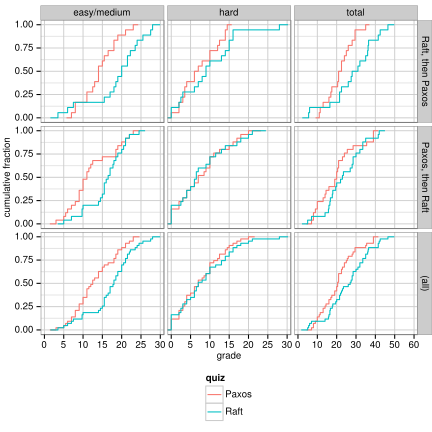
\includegraphics{userstudy/diffBreak}
}
\vspace{-4ex}
\vcaption[quiz score CDFs by question difficulty and ordering]{
CDFs of 43 participants' quiz scores, broken down by question difficulty
and ordering. 
Each curve shows the fraction of participants who scored up to
that many points (right/lower is better).
The \emph{total}, \emph{(all)} graph is
identical to Figure~\ref{fig:userstudy:unpairedcdf}.

\textbf{Difficulty:}
The \emph{easy/medium} column shows the participants' scores for the easy and
medium questions on the quiz, out of a maximum possible \SI{30}{points}.
The \emph{hard} column shows the participants' scores for the hard
questions on the quiz, out of a maximum possible \SI{30}{points}.
The \emph{total} column shows the participants' total scores, out of a
possible \SI{60}{points}.
Figure~\ref{fig:userstudy:breakdown} breaks this down by individual question.

\textbf{Ordering:}
The \emph{Raft, then Paxos} row shows the scores for the
participants who took the Raft quiz before taking the Paxos quiz.
The \emph{Paxos, then Raft} row shows the scores for the
participants who took the Paxos quiz before taking the Raft quiz.
The \emph{(all)} column shows the scores for all participants who took
both quizzes.
}
\label{fig:userstudy:diffBreak}
\end{figure}

Figure~\ref{fig:userstudy:diffBreak} shows distributions of quiz scores broken
down by question difficulty. There were only \SI{4}{points} of Easy questions,
so we combined those with the Medium category in the graphs.
The graphs show that almost all of the difference
in scores can be attributed to questions in the Easy/Medium category,
and the Hard category accounted for only a very small difference in
scores. We made the hard questions too difficult: on average,
participants scored only about one quarter of the possible points in the
Hard category (\SI{7.45}{points} on average on Paxos and
\SI{7.94}{points} on
average on Raft). Thus, we were unable to measure much difference
between participants in the Hard category.

\begin{figure}
\centering
{
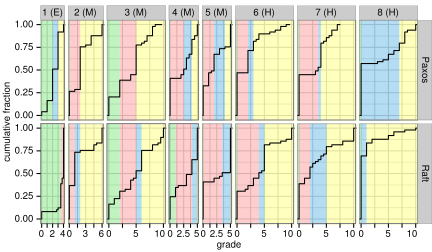
\includegraphics{userstudy/breakdown}
\vspace{-1ex}\\
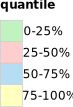
\includegraphics{userstudy/breakdownlegend}
}
\vcaption[quiz score CDFs by question]{
CDFs of participants' scores on individual questions.

Each graph in the figure shows the quiz scores for an individual quiz
question. The top row of graphs shows Paxos quiz questions; the bottom
row shows Raft quiz questions. The number above each graph is the number
of the question (multi-part questions have been aggregated to save
space).

The curve in each graph shows a CDF of the data. The
\emph{y} axis is the cumulative fraction of participants who scored up
to a given number of points (right/lower is better).

The range of the \emph{x} axis on each graph corresponds to the
point values possible for each question, and one point has the same width
in every graph. For example, the graph for a 10-point question is twice
as wide as the graph for a 5-point question.

Each graph is also colored to provide summary information at a glance.
Each quantile of the data is shaded in a different color, as shown
in the legend. Because each graph's width is scaled to its point value,
the size (area) of the shading is proportional to the number of points
it represents.
}
\label{fig:userstudy:breakdown}
\end{figure}

Figure~\ref{fig:userstudy:breakdown} breaks the quiz scores down by individual
question. Question 1 was Easy difficulty, Questions 2 through 5 were
Medium difficulty, and Questions 6 through 8 were Hard difficulty, based
on our categorization. There do not appear to be any individual
questions in the Medium category that alone account for large
differences. Although we tried to pair question difficulty across
quizzes (for example, Q3 on the Raft quiz should be about as difficult
as Q3 on the Paxos quiz), they are mostly different questions that are
hard to compare directly.

\subsection{Survey}
\label{userstudy:results:survey}

Participants answered three groups of survey questions after taking their
second quiz.
The questions asked
about their prior experience with Paxos and Raft,
whether they felt the lectures or quizzes were biased, and which
algorithm they felt would be easier to implement or explain.
Participants were also asked for open-ended comments or feedback.
The full survey and exact questions can be found in
Appendix~\ref{appendix:userstudy:survey}, along with the open-ended
comments and feedback.

\begin{figure}
\centering
{
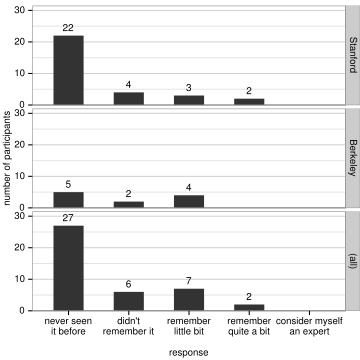
\includegraphics{userstudy/surveypaxos}
}
\vcaption[prior Paxos experience survey]{
Prior Paxos experience survey.
Using a five-point scale, participants were asked how much prior exposure
they had to Paxos; 42 participants responded to the question.
The top graph shows the responses from the Stanford participants, the
middle graph shows the responses from the Berkeley participants, and the
bottom graph shows the total responses (from all participants).
}
\label{fig:userstudy:surveypaxos}
\end{figure}

Many of the Berkeley participants and some of the Stanford participants
had prior exposure to Paxos; Figure~\ref{fig:userstudy:surveypaxos} shows
their responses to the survey question. At Stanford, 9 of the 31
participants who responded to the question had at least some prior
exposure to Paxos. At Berkeley, 6 of the 11 participants who
responded to the question had at least some prior exposure to Paxos.
No participants reported any prior exposure to Raft (41 participants
responded to this question); Raft was still new at the time, so this was
expected.

\begin{figure}
\centering
{
\includegraphics{userstudy/surveyfair}
}
\vcaption[fairness survey]{
Fairness survey.
Using a five-point scale, participants were asked which lecture was better
and which quiz was more difficult.
42 participants responded to each question.
\\
\textbf{Left:}
Do you think the video lectures were roughly equal in quality, given the
nature of the material being presented?
\\
\textbf{Right:}
Do you think the quizzes were roughly equal in terms of testing your
understanding of the material?
\\
The top graphs show the responses from the Stanford participants, the
middle graphs show the responses from the Berkeley participants, and the
bottom graphs show the total responses (from all participants).
}
\label{fig:userstudy:surveyfair}
\end{figure}

Participants were also asked whether they felt the lectures were of
similar quality and whether the quizzes were of similar difficulty;
Figure~\ref{fig:userstudy:surveyfair} shows their responses.
23 of 42 participants responded that the Raft lecture was at least
somewhat better than the Paxos lecture, and 20 of 42 participants
responded that the Paxos quiz was at least somewhat harder than the Raft
quiz.
However, these responses may be unreliable: it may have been difficult
for participants to separate
the intrinsic difficulty of the material or
their level of understanding from the
lecture quality, or their performance from the quiz difficulty.
Therefore, we do not consider this strong evidence against the integrity
of our study.

\begin{figure}
\centering
{
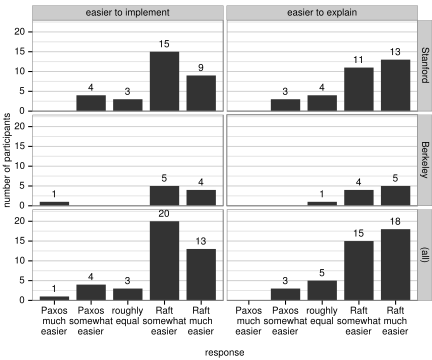
\includegraphics{userstudy/survey}
}
\vcaption[preferences survey]{
Preferences survey.
Using a five-point scale, participants were asked which algorithm would be
easier to implement and which would be easier to explain.
41 participants responded to each question.
\\
\textbf{Left:}
Suppose you were working at a company and it is your job to implement a
replicated state machine. Which algorithm would be easier to implement in a
functioning, correct, and efficient system?
\\
\textbf{Right:}
Suppose you had to explain either Raft or Paxos to a CS graduate student who
hadn't seen either one previously. Which would be easier to explain?
\\
The top graphs show the responses from the Stanford participants, the
middle graphs show the responses from the Berkeley participants, and the
bottom graphs show the total responses (from all participants).
}
\label{fig:userstudy:survey}
\end{figure}

Figure~\ref{fig:userstudy:survey} shows which algorithms participants felt would
be easier to implement or explain. An overwhelming majority of
participants preferred Raft for each: 33 of 41 participants reported
that Raft would be at least somewhat easier to implement, and 33 of 41
participants reported that Raft would be at least somewhat easier to
explain.
However, these self-reported feelings may
be less reliable than participants' quiz scores, and participants may
have been biased by knowledge of our hypothesis that Raft is easier to
understand.

%


\section{Discussion about the experimental approach}
\label{userstudy:approachdiscussion}

Initially, we doubted that a user study would be feasible or convincing,
but we felt it was the most appropriate way to evaluate Raft's claim of
understandability. Thus, we conducted the user study to provide
empirical evidence that Raft is easier to understand than Paxos.
Although we consider the study itself successful, it
was not particularly well-received by the system community.
This section explores whether the study was
worth the time and effort we put into it and sheds light into whether
this sort of experiment is effective in the systems community.

In our first paper submission on Raft (in 2012),
we claimed the Raft algorithm was
easier to understand than Paxos, but we had essentially no objective
evidence for this. Our anonymous reviewers rightly pointed out this
weakness. Excerpts from their reviews serve as evidence that with no
evaluation, our claim of understandability was weak:
\begin{itemize}
\em
\item It's not clear Raft is any more understandable than Paxos. While
understandability is the key claim to novelty, this claim was not
actually evaluated, and may be untrue.\ \ldots\ 
I think one thing that would have helped a lot is if the authors chose a
concrete ``metric of success'' and evaluated their system according to
that metric.\ \ldots\ 
I do like the idea of using understandability as a metric, but that [sic]
there was no attempt at all to actually characterize Raft using that
metric.

\item
\ldots\ I understood the algorithm. So, perhaps that speaks to the fact
that Raft is indeed understandable.

That said, I do think that you [need] a way to show that Raft is indeed
more understandable. A couple of thoughts on doing that:

\begin{compactitem}
\item Compare implementations of Raft and Paxos using some code
complexity measures.
\item Explain Raft and Paxos to students, and see which one they
understand better. A test of understanding could be writing the
pseudocode, a quiz on algorithm behavior, or extending the algorithm to
do something different.
\end{compactitem}

\item We encourage the authors to define metrics for
``understandability'' and systematically explore whether the protocol
meets these goals.\ \ldots
\end{itemize}


Based of this feedback, we conducted the Raft user study and included
its results in our second paper submission. Unfortunately, the study did
not seem to convince most of our reviewers; they did not seem to find
much value in it. Several did not even mention it in their reviews.
Others were concerned about the lecture content and quiz questions, even
though we referred our readers to the user study lectures and quizzes
online. The paper was ultimately accepted (in 2014) after several attempts, but
we feel this was despite the reviewers' generally negative opinions of
the study. The following excerpts summarize the reviewers' opinions
about the user study:

\begin{itemize}
\em


\item The user study is not that useful.

\item The evaluation is thin.  Its qualitative thesis (Raft is simpler
$\Rightarrow$ Raft is more understandable $\Rightarrow$ Raft
implementations are more correct) is poorly supported, and hence subject
to the reader's counter intuition.\ \ldots\ 
This paper's evaluation hinges on the user study. Did the tests test the
corner cases? Did the students have to prove either system correct,
formally?

\item I'm disappointed that Section 7 [Clients and log compaction] is
empty! Given a choice, I'd rather omit Section 8 [Implementation and
evaluation] and include Section 7.

\item The user study is a nice idea, but ultimately I don't think it
adds much to the paper. Readers will decide for themselves if the
algorithm is understandable or not and the paper's ultimate impact will
depend on this judgement, not a user study.



\item The user study is interesting.

Unclear whether explaining Paxos more clearly would change the
results of the user study.

\item Reasonable user study about ``understandability''.

User study, while laudable, seems fairly unscientific in the end due
to potential large sources of bias.

I appreciate the author's attempts to better characterize
whether Raft is indeed ``more understandable'' than Paxos, and care was
put into designing the study (e.g., splitting users, presenting them
with tests is different orders, etc.).  Even so, if our goal is really
randomized trials, the fact that the experimenters wrote the
explanations of the two protocols gives me some real pause about some
pretty overt bias that could slip into the writeup.

\item User study is fresh and interesting (albeit bias factors are present).

The user study is interesting and thought provoking, but it really lacks
representativeness both in terms of sample sizes as well as neutrality.

\item I think the understandability study is interesting, but perhaps a
little bit of overkill.  Typically researchers can compare two protocols
and see for themselves which is simpler \ldots
But I'm not against a little overkill now and then.  However,
summarizing a study with a statement such as ``students were able to
answer questions about Raft 23\% better than questions about Paxos''
raises immediate questions about whether such figure is very meaningful.
In particular 23\% seems like a precise figure, but in fact depends a lot
on how the tutorials and the test are set up (even when strong measures
are taken to ensure fairness, as you have done).  Two issues that come
to mind are that you can't ask exactly the same questions about two
different protocols, and even if you could, it's not clear which
questions would be the right or fair questions to ask to get at the
issue of understandability.

\item The user study based on self-reported understandability scores and
correctness of answering problem questions is not particularly
convincing. It would be more convincing if students were made to
implement both Paxos and Raft in code, and then compare objectively the
time taken, the lines of code, and the overall correctness.

Concrete suggestion: Please provide some objective measure on
understandability, even if it is for a small sample-set of students that
implement both Paxos and Raft from just communication primitives.



\item I found the sample size in the section on understandability to be
small enough to be worrisome in spite of the good t-test number.  A
better test might be the number of unaccounted for failure modes in
na\"ive implementations.  I expect Raft to win by a wide margin.

\item 
Furthermore, a review of the teaching materials in~\cite{study} seems to
indicate flaws in the way the ``Understandability study'' was
performed. Some implementations of Multi-Paxos support concurrent
proposals which are ordered by the leader. However, it is unclear how
Raft does the same. From the description in the paper, I think Raft
handles Append entries (performing Append RPCs) sequentially. So,
aren't you comparing the understandability of 2 algorithms with
different properties?

\item I find the evaluation of using students' feedback interesting.
However, it's hard to be convinced of your conclusion if I don't know
what quizzes are being asked.

\item The authors evaluation of the subjective claim of
understandability was done valiantly in section 8.1 [Understandability],
bravo.

\item We [reviewer and students] didn't like the user study. It's not
necessary or convincing. Adding more information to make it convincing
would not be worth the space cost.

\end{itemize}

Moreover, conducting the Raft user study was inherently costly and risky
in terms of time and effort. Typically, systems papers evaluate their
performance quantitatively through machine experiments; such experiments
have low cost and fast turnaround. This results in several attractive
properties as compared to psychology experiments involving human
subjects:
\begin{itemize}
\item \textbf{Repeatability:} Performance evaluations are typically
easy and cheap to repeat. They are often automated so that there is
little room for experimenter error in repeating the experiment. On the
other hand, psychology experiments require much more human involvement
in general, making them more costly and more error-prone to repeat.
\item \textbf{Iteration:} Easily repeatable experiments make it possible
to change the system, its environment, or the experiment based on
experimental results. For example, a researcher might discover a bug
during performance evaluation, fix it, and rerun the experiments, at
little or no additional cost. This can be prohibitively costly in a psychology
experiment, as it requires restarting the entire study with a new group
of participants.
\item \textbf{Incremental results:} In a user study, almost all of the
work must be done before seeing any results, or even learning whether
the basic idea makes sense. This makes such experiments much riskier
than performance evaluations, where initial coarse-grained results are
often attainable with little effort.
\end{itemize}

On the other hand, novel approaches can bring some of these properties
to human subjects psychology experiments. For example in one study, Dow
\emph{et al.}~\cite{Dow:2010} compare ad impressions using web
analytics. This is objective, repeatable, allows iteration, and is
incremental. Similar techniques may apply to evaluating
understandability in some domains. Massive open online courses (MOOCs)
may also be a useful experimental platform for understandability by
providing researchers with pools of thousands of students to teach and
evaluate.


Despite reviewers' concerns, we consider the user study to be an
essential part of this work. Its results are the only objective evidence
we have that Raft is easier to understand than Paxos. The results assume
that the study's lectures are of equal quality and that its quizzes are
of equal difficulty. Though we have no way to prove this, the methods
aimed to produce equivalent lectures and quizzes, and the materials are
available for readers to review. Under this assumption, the results
should be convincing, even to skeptical readers.


\section{Conclusion}

The Raft user study compared Raft's understandability to that of Paxos.
The study showed that after learning Paxos or Raft for an hour,
students are able to answer equally difficult questions about Raft
better than they can about Paxos. We believe we countered all major
sources of bias in our study, and the study showed the major result we
wanted. However, it took significant time and effort. We hope future
techniques, such as leveraging online courses, allow studies to achieve
similar results at a lower cost.

The Raft user study was unconventional for systems research, which tends
to focus on machine-based performance evaluations. Our study provides
substantial evidence in favor of Raft's understandability, and as far as
we know, it is the first study to objectively evaluate consensus
algorithms based on teaching and learning. We believe the systems
community should carefully consider such studies, as they enable us to
advance our collective knowledge through novel kinds of contributions
that we could not otherwise convincingly evaluate.

\chapter{Correctness}
\label{correctness}

Since the purpose of consensus is to maintain consistency across a
replicated state machine, correctness is a key concern. Not only must
the algorithm itself be correct, but others must also be able to
implement it correctly in real systems. We took a pragmatic approach to
correctness in Raft, building a foundation through understanding and
intuition, then applying formal methods to the degree they were
practical.

To establish the correctness of Raft itself, we developed a formal
specification for the basic Raft algorithm and a proof of its safety.
These are described in Section~\ref{correctness:specproof} and can be
found in full in Appendix~\ref{appendix:correctness}. Although many
other components are needed for a complete system (specifically,
membership changes, log compaction, and client interaction), this is an
important step towards proving Raft correct.
Section~\ref{correctness:prior} discusses other methods we tried before
arriving at the current proof.

Our goal is for others to be able to build correct systems using Raft,
and Section~\ref{correctness:testing} describes approaches to doing so.
We hypothesize that systems builders will have an easier time developing
correct implementations if they fully understand Raft; this is another
reason why understandability is so important. We have tried to be clear
and precise in describing Raft, but one problem with natural languages
is that they can easily be imprecise or ambiguous. Thus, we encourage
system builders to compare their understanding with Raft's formal
specification, which is completely precise using mathematical language.

\section{Formal specification and proof for basic Raft algorithm}
\label{correctness:specproof}

We have developed a formal specification and a proof of safety for the
consensus mechanism described in Chapter~\ref{basicraft}; these can be
found in Appendix~\ref{appendix:correctness}.
The formal specification makes the information summarized in
Figure~\ref{fig:basicraft:cheatsheet} completely precise using the TLA+
specification language~\cite{Lamport:2002}. It is about \num{450} lines long
and serves as the subject of the proof.
It is also useful on its own for anyone implementing
\name{}.

The formal specification defines the state in a complete Raft cluster
with an arbitrary number of servers. It defines an initial state
(\emph{Init}) in which all the servers' logs are empty and defines all
possible transitions from one state to another (\emph{Next}). There are
several such transitions: the network may duplicate or drop a message,
and a server may (under the right conditions) receive a message,
timeout, restart, become a leader, advance its commit index, receive a
request from a client, send a RequestVote request, or send an
AppendEntries request. Each transition includes the conditions under
which it may occur. For example, a server may only request a vote if it
is in the candidate state.

The specification models an asynchronous system (it has no notion of
time) with the following assumptions:
%
\begin{itemize}
%
\item Messages may take an arbitrary number of steps (transitions) to
arrive at a server. Sending a message enables a transition to occur (the
receipt of the message) but with no particular timeliness.
%
\item Servers fail by stopping and may later restart from stable storage
on disk.
%
\item The network may reorder, drop, and duplicate messages.
%
\end{itemize}

The formal specification is slightly more general than the Raft
algorithm presented in Chapter~\ref{basicraft}. These differences make
the formal specification applicable to a wider range of implementations
and also make some of its state transitions more orthogonal, which
simplifies the proof. One way in which the formal specification differs
from the algorithm's description is that it uses message-passing rather
than RPC. This requires a minor change to the AppendEntries response
format, but it eliminates the need to pair responses with requests.
The specification also takes more transitions than most
implementations would to arrive at the same end state. Since each
transition is evaluated atomically, this models smaller atomic regions
in an implementation. There are several examples of this:
%
\begin{itemize}
%
\item When a server times out, it does not grant itself a vote in the
same step. Instead, it requests its own vote with an asynchronous
RequestVote request message. Also, after a candidate receives its final
vote, it becomes leader in a separate transition.
%
\item Leaders do not advance their commit index upon receiving an
AppendEntries reply. Instead, they do so in a separate transition. This
improves orthogonality, since a leader that forms a single-server
cluster can also increase its commit index through the same transition.
%
%
\item On receiving an AppendEntries request, a server either returns to
the follower state, truncates just the last entry from the end of its
log, appends just one entry to the end of its log, or replies in one
atomic step (it can then continue to process the request in further
steps). Reducing
this atomic region to just one entry at a time turns out to be important
for implementations that write to persistent storage. For example, when
entries span multiple files, most file systems would not allow
truncating all of the entries atomically. The specification shows that
implementations may safely truncate the entries back to front, one or
more at a time.
%
\item Servers update their current terms and states upon receiving a
message with a larger term, then in a different transition they process
the message.
%
\end{itemize}
%
On the other hand, the specification is not as general as possible; that
would harm its understandability. For example, some transitions set two
variables even when they need not be set atomically.

The proof verifies the State Machine
Safety property. It is complete (it relies on the specification alone)
and relatively precise (it is about \num{3500} words long). The main idea
of the proof is summarized in Section~\ref{basicraft:safety:argument}.
Most of the lemmas (subproofs) show that an invariant holds for all states that
are reachable from the initial state in an execution. Using induction,
they assume the invariant holds in one state and show that it holds in
every possible next state.

It is often necessary in the proof to refer to variables from prior
states in the execution. To make this precise, the specification is
augmented with {\em history variables}; these variables carry
information about past events forward to states that follow. For
example, one history variable called $elections$ maintains a record of
every successful election in the execution, including the complete log
of each server at the time it cast its vote and the complete log of the
new leader. The history variables are never read in the specification
and would not exist at all in a real implementation; they are only
``accessed'' in the proof.

\section{Discussion of prior verification attempts}
\label{correctness:prior}

Prior to arriving at the current proof, we tried three other approaches:
%
\begin{enumerate}
%
\item We first checked an earlier version of Raft in the Murphi model
checker~\cite{Dill:1992}, which explores the complete state space to
check for unsafe conditions. The state space quickly expanded to the
point where Murphi could not finish (in a reasonable amount of
time), so we had to limit the size of the
system to at most four entries in each log, four terms, and five
servers. Murphi found one bug in an early version of Raft, which caused
log inconsistencies when multiple leaders in a row crashed after
incompletely committing log entries.
It also missed an important bug in an early version of Raft,
where the commitment rule did not account for scenarios like that of
Figure~\ref{fig:basicraft:oldTermCommit}.
Murphi most likely missed this bug because of the constrained model size
(fortunately, David \mazieres{} found it).
%
\item We attempted to use the TLA model checker on our specification. We
found bugs in creating the specification this way but
abandoned this approach because it did not scale well to larger models.
%
\item We also attempted to use the TLA proof
system~\cite{Cousineau:2012}, which introduces a hierarchical language
for formally proving properties on TLA specifications and includes a
machine checker for such proofs. We mechanically proved the Leader
Completeness Property using the TLA proof system, but this proof relied
on invariants that have not been mechanically checked (for example, we
did not prove the type safety of the specification). Unfortunately, we
found it too tedious and time-consuming to use the TLA proof system at
the scale of a complete proof. One problem is that TLA is untyped,
making it more general but also more tedious~\cite{Lamport:1999}.
%
\end{enumerate}

We found the tools for correctness to be limited in various ways. In our
experience, model checking was orders of magnitude easier than
developing a proof. It essentially requires writing a simplified Raft
implementation, and then it can be executed and debugged even easier
than a distributed system (model checkers output a full execution trace
when any problems occur). Unfortunately, we were not able to verify our
models with large enough parameters to be fully convinced of their
correctness.

On the other hand, the Raft proof took about six weeks  of learning
and thinking before any significant progress was made. Creating a proof
takes a different skill set from programming and a different sort of
creativity. The end result has helped build our confidence in Raft's
safety, but the proof might have bugs. At the scale of the complete Raft
specification, only a mechanically checked proof could definitively be
bug-free. We think a machine-checked proof for Raft would be feasible
with more capable tools (e.g, Coq~\cite{Bertot:2004}), and one has
recently been created for Multi-Paxos~\cite{Schiper:2014}. However, the
time investment required would probably be on the order of several
months.

\section{Building correct implementations}
\label{correctness:testing}

There are many possible approaches to building a correct implementation
of Raft. The safest approach is to generate an implementation
automatically from a proven Raft specification. If the tools are
correct, this guarantees that there will be no errors in converting the
specification to an implementation. Recent work has shown this to be
feasible for Multi-Paxos~\cite{Schiper:2014}, and we expect it to be for
Raft as well. However, this approach has not been very popular in
practice so far, perhaps because real-world systems have additional
needs, such as performance, that are harder to accommodate in the
generated code.

Without generating an implementation, implementers should strive to
design their implementations to reduce the possibility of creating bugs,
and they should test their implementations to reduce the possibility of
encountering bugs in production. The remainder of this section discusses
several approaches we think may be effective, though we have not
evaluated their effectiveness. Readers may also be interested in the
testing strategy used for Chubby~\cite{Chandra:2007}.

Howard describes a nice design for building ocaml-raft
correctly~\cite{Howard:2014,impl:ocaml-raft}. It collects all the Raft
state transitions in one module, while all code for determining when
transitions should occur is elsewhere. Each transition checks its
pre-conditions using assertions and has no system-level code
intermixed, so the code resembles the core of the Raft specification.
Because all of the code that manipulates the state variables is
collected in one place, it is easier to verify that state variables
transition in restricted ways. A separate module invokes the transitions
at the appropriate times.
Moreover, ocaml-raft can simulate an
entire cluster in a single process, which allows it to assert Raft's
invariants across virtual servers during execution. For example, it can
check that there is at most one leader per term at runtime. 

For end-to-end testing, Jepsen and Knossos are useful tools that have
already found bugs in two Raft implementations (in read-only request
handling)~\cite{Kingsbury:etcdconsul}. Jepsen injects network partitions
in a distributed system and determines whether the system loses data.
Knossos analyzes clients' histories of operations against a distributed
system to look for ways those histories are not linearizable. Together,
these can be used as powerful end-to-end tests for Raft systems.

Some of the most difficult to find bugs are those that only occur in
unlikely circumstances such as during leadership changes or partial
network outages. Thus, testing should aim to increase the likelihood of
such events. There are three ways to do this.

First, Raft servers can be configured to encourage rare events for
testing. For example, setting the election timeout very low and the
heartbeat interval very high will result in more leader changes. Also,
having servers take snapshots very frequently will result in more
servers falling behind and needing to receive a snapshot over the
network.

Second, the environment can be manipulated to encourage rare events for
testing. For example, servers can be randomly restarted and cluster
membership changes can be invoked frequently (or continuously) to
exercise those code paths. Starting other processes to contend for
servers' resources may expose timing-related bugs, and the network can
be manipulated in various ways to create events that occur only rarely
in production, such as:
%
\begin{compactitem}
%
\item Randomly dropping messages (and varying the frequency of drops
between servers and links);
%
\item Adding random message delays;
%
\item Randomly disabling and restoring network links; and
%
\item Randomly partitioning the network.
%
\end{compactitem}

Third, running the tests for a longer period of time will increase the
chance of discovering a rare problem. A larger number of machines can
run tests in parallel. Moreover, entire clusters can run as separate
processes on a single server to reduce network latency, and disk
overheads can be reduced by persisting to RAM only (for example, with a
RAM-based file system such as tmpfs~\cite{tmpfs}). While not entirely
realistic, these techniques can exercise the implementation aggressively
in a much shorter period of time.

\section{Conclusion}

We believe our evaluation of Raft's correctness puts it at least on par
with the algorithms used in most Paxos-based systems. Theoreticians have
typically proven the safety of only narrow specifications of Paxos, but
practitioners deviate from these specifications and extend their systems
significantly. The formal specification for Raft is a nearly complete
implementation of the basic Raft algorithm presented in
Chapter~\ref{basicraft}, so the fraction of a fully elaborated Raft
algorithm that has been proven safe is fairly large. We leave specifying
and proving cluster membership, log compaction, and client interaction
to future work, along
with liveness and availability properties of the basic Raft algorithm.

\chapter{Leader election evaluation}
\label{leaderelection}

\newcommand\algo[1]{\emph{#1} algorithm}
\newcommand\algocap[1]{\emph{#1} algorithm}
\newcommand\algoabbrv[1]{\emph{#1} algo.}

This chapter analyzes the performance of leader election in Raft, which
occurs when a leader fails and needs to be
replaced. Although we expect leader failures to be a rare event, they
should be handled in a timely manner. We would like Raft to reliably
elect a new leader in a fraction of a second in a typical deployment.

Unfortunately, it is difficult to put a bound on the time or number of
messages leader election will take. According to the FLP impossibility
result~\cite{Fischer:1985}, no
fault-tolerant consensus protocol can deterministically terminate in a
purely asynchronous model. This manifests itself in split votes in Raft,
which can potentially impede progress repeatedly during leader election.
Raft also makes use of
randomized timeouts during leader election, which makes its analysis
probabilistic. Thus, we can only say that leader election
performs well with high likelihood, and even then only under various
assumptions. For example, servers must choose timeouts from a random
distribution (they are not somehow synchronized), clocks must proceed at
about the same rates, and servers and networks must be timely (or
stopped). If these assumptions are not met for some period of time, the
cluster might not be able to elect a leader during that period
(though safety will always be maintained).

This chapter draws the following conclusions about the performance of
Raft's leader election algorithm:
%
\begin{itemize}
%
\item When no split vote occurs, elections complete about one third of
the way into the election timeout range, on average. They complete
slightly faster in clusters with more available servers, since the first
server is expected to time out sooner.
(Section~\ref{leaderelection:nosplit})
%
\item Split vote rates are low when the election timeout range is
sufficiently broad. We recommend a range that is
10--20 times the one-way
network latency, which keeps split votes rates under 40\% in all cases
for reasonably sized clusters, and typically results in much lower rates.
Clusters will experience more split votes as more servers fail, since
fewer votes are available. (Section~\ref{leaderelection:split:rate})
%
\item The number of election terms required to elect a leader follows a
geometric distribution,
where the expected number is $\dfrac{1}{1-\text{split vote rate}}$.
Thus, even a high split vote rate of 50\% will only need two election
terms on average to elect a leader.
A cluster configured with an election timeout that is 10--20 times its
one-way network latency will be able to elect a leader in less than 20
times its one-way network latency on average.
(Section~\ref{leaderelection:split:total})
%
\item Leader election performs well in practice in both local and wide
area networks. In a real-world LAN, our system was able to elect a
leader in an average of \SI{35}{\milli\second} when configured with aggressive
timeouts, though we suggest using a more conservative timeout range in
practice. On a simulated WAN spanning the US, elections typically
complete in half a second, and 99.9\% of elections complete in
\SI{3}{seconds}, even when two of five servers have failed.
(Section~\ref{leaderelection:lan})
%
\item The performance of leader election is not substantially affected
by the log comparison in RequestVote RPCs, when some servers will not
grant their votes to others. (Section~\ref{leaderelection:logsdiff})
%
\item The basic leader election algorithm can cause disruptions if
followers lose connectivity, increment their terms, and then regain
connectivity. Section~\ref{leaderelection:prevote} extends the basic
algorithm with an additional phase to avoid such disruptions.
%
\end{itemize}

\section{How fast will Raft elect a leader with no split votes?}
\label{leaderelection:nosplit}

\begin{figure}
\centering
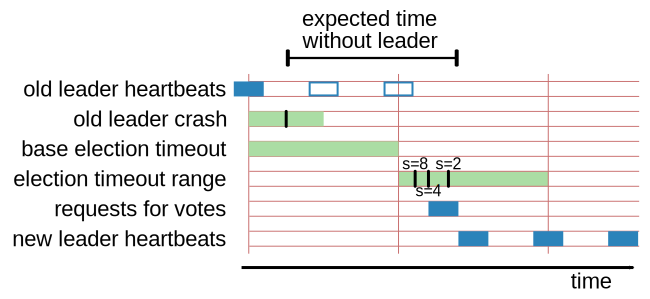
\includegraphics[scale=.55]{leaderelection/timeline}
\vcaption[leader election timeline with no split votes]{
Timeline of a typical election when no split vote occurs.
The first candidate to time out successfully collects votes and
completes the election (other elections may not be so fortunate). The
figure is drawn to scale assuming the election timeouts are chosen from
a range between 10--20 times the cluster's one-way network latency.
\\
The ``old leader heartbeats'' row shows the final heartbeat that the
old leader completes, and when it would have sent its next heartbeats
were it not to crash.
\\
The ``old leader crash'' row shows the interval during which the old
leader crashes. This time is assumed to follow a uniform random
distribution within its heartbeat interval. The vertical line halfway
through the interval is its expected (average) value.
\\
The ``base election timeout'' row shows the interval during which all
the followers await additional heartbeats from the old leader.
\\
The ``election timeout range'' row shows the interval during which the
servers would time out and start elections to replace the old leader.
The vertical lines show expected earliest timeout values for different
numbers of remaining servers (eight, four, and two, respectively).
\\
The ``requests for votes'' row shows when the candidate sends its
RequestVote RPCs to the other servers and receives their votes.
\\
The ``new leader heartbeats'' row shows the new leader sending out
heartbeat RPCs right away after becoming leader, then periodically
thereafter.
}
\label{fig:leaderelection:nosplit:timeline}
\end{figure}

The most common case for leader election in Raft is when no split vote
occurs, and this section analyzes how long it takes to elect a leader
under that assumption. This is expected to be the normal case for Raft
clusters; if the cluster is configured correctly, most normal elections
will not encounter a split vote. The first server to time out will be
able to collect votes from a majority of the cluster and become leader.
The timeline of events is shown in
Figure~\ref{fig:leaderelection:nosplit:timeline}. 

\begin{table}
\centering
\begin{tabular}{ccl}
variable & type & meaning \\
\hline
\noalign{\vskip .75ex}
$s$     & natural & number of available servers \\
$n$     & natural & size of full cluster (including unavailable servers) \\
$c$     & natural & number of servers to time out near each other \\
$l$     & time & constant half round trip network latency (special case of $L$)\\
$L$     & random variable of time & half round trip network latency \\
$W$     & random variable of time & time to write term and vote durably to disk \\
$T_i$   & random variable of time & timeout of server $i$ \\
$M_s$   & random variable of time & earliest timeout of $s$ servers \\
$D_{c,s}$ & random variable of time & difference in timeouts of earliest $c$ of $s$ servers \\
$E_s$   & random variable of time & time to complete an election \\
\end{tabular}
\vcaption[summary of variables]{
Summary of the variables used throughout this chapter to
analyze leader election performance.
Times are normalized to the election timeout range (ranging from 0 to
1).
}
\label{tab:leaderelection:variables}
\end{table}

\begin{figure}
\centering
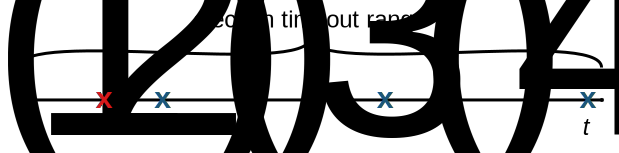
\includegraphics[scale=.5]{leaderelection/earliesttimeoutdiagram}
\vcaption[earliest timeout example]{
What is the smallest random election timeout value chosen by $s$
servers? The diagram shows random election timeouts a five-server
cluster where one server has failed ($s=4$). $t_{(1)}$ is the smallest
timeout value chosen.
}
\label{fig:leaderelection:theory:earliesttimeoutdiagram}
\end{figure}

With no split votes, the time it takes to elect a leader is determined
by how long it takes the first server to time out. The question of when
it will time out is illustrated in
Figure~\ref{fig:leaderelection:theory:earliesttimeoutdiagram}. Each server
waits for a uniform random timeout after the last time it received a
heartbeat. Intuitively, any individual server is expected to time out
halfway through the election timeout range, but with more servers it
becomes more likely that the first server will time out sooner.

We now define the problem more precisely and derive when the first
server times out analytically. The variables defined in this chapter are
summarized in Table~\ref{tab:leaderelection:variables}. Suppose each
server chooses its timeouts randomly from the standard
uniform distribution (in the range $[0,1]$). Let $T_1 \ldots T_s$ be
random variables representing when each of $s$ servers times out. Let $M_s$ be the minimum of
$T_1 \ldots T_s$, a random variable representing the time the first
server times out. Its cumulative distribution function (CDF) defines the
probability that $M_s$ is no greater than a particular time, $t$. This
is equivalent to one minus the probability that all servers times out
after $t$:
\begin{align*}
\Pr(M_s \leq t)
        &= 1 - \Pr(M_s > t) \\
        &= 1 - \prod_{i=1}^s \Pr(T_i > t) \\
        &= 1 - \prod_{i=1}^s (1 - t) \\
        &= 1 - (1-t)^s
\end{align*}
%
For example, consider a cluster with five servers where the prior
leader has failed.
The probability that the earliest of the remaining four servers times out
sometime in the first quarter of the election timeout range is
$\Pr(M_4 \leq \frac{1}{4}) = 1 - (1 - \frac{1}{4})^4 \approx 0.68$.
The CDF is graphed in
Figure~\ref{fig:leaderelection:theory:model:earliesttimeout}
for various values of $s$.

\begin{figure}
\centering
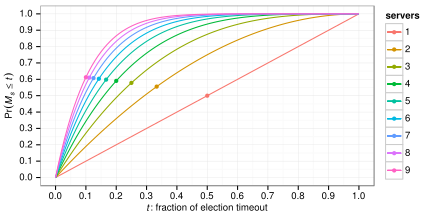
\includegraphics{leaderelection/earliesttimeout}
\vspace{-2ex}
\vcaption[earliest timeout CDF]{
The graph shows the probability that the earliest server times out
before $t$ when different numbers of servers are available. The point on
each line shows the time when the first server is expected to time out
($\Ex[M_s]$).
}
\label{fig:leaderelection:theory:model:earliesttimeout}
\end{figure}

The probability density function (PDF) of $M_s$ is the derivative of the
CDF:
\begin{align*}
 f_{M_s}(t) &= \frac{d}{dt} \Pr(M_s \leq t) \\
        &= \frac{d}{dt} (1-(1-t)^s) \\
        &= -\frac{d}{dt} (1-t)^s \\
        &= s (1-t)^{s-1}
\end{align*}

The expected value (mean) of $M_s$ is calculated from the PDF:
\begin{align*}
 \Ex[M_s] &= \int_0^1 \! t \, f_{M_s}(t) \, dt \\
          &= \int_0^1 \! t (s (1-t)^{s-1}) \, dt \\
          &= \left. \! -\frac{(1-t)^s (s\,t+1)}{s+1} \right|_{t=0}^1 \\
          &= \frac{1}{s+1}
\end{align*}

\noindent
For example, with four available servers, the first timeout is expected
to occur $\dfrac{1}{5}^\textrm{th}$ of the way through the election
timeout range. Fortunately, this very simple expression is a good
estimate of Raft's overall election performance, since elections
complete soon after the first candidate times out when no split vote
occurs.

More precisely, if there is no split vote, the full election requires
a candidate to time out and request votes, once the leader crashes:
\begin{align*}
E_s &= \text{baseline election timeout} + M_s + \text{time to request
votes} - \text{heartbeat adjustment} \\
E_s &= 1 + M_s + 2L + W - U(0,\dfrac{1}{2}) \\
\Ex[E_s] &= 1 + \frac{1}{s+1} + 2\Ex[L] + \Ex[W] - \dfrac{1}{4}
\end{align*}
where election timeouts are chosen from the range $[1,2]$,
$L$ is the network latency, and $W$ is the time to write the votes
persistently to disk.
A uniform random time value from the range $[0, \dfrac{1}{2}]$ is
subtracted, since leaders are expected to crash randomly within their
heartbeat intervals rather than immediately after sending heartbeats.

\section{How common are split votes?}
\label{leaderelection:split:rate}

The previous section analyzed the performance of normal elections when
no split vote occurs. In practice, two or more candidates may time out
at similar times, leading to split votes.  Split votes cause additional
election timeout delays, and if they occur too frequently, they can
impact election performance dramatically. This section first analyzes
split votes under a simplifying assumption that network latencies are
constant, then subsequently relaxes this assumption.

\subsubsection{Split vote rate with fixed latency}

\begin{figure}
\centering
\includegraphics[scale=.5]{leaderelection/splitvotediagram}
\vcaption[split vote example with fixed latency]{
These examples show two similar elections in a five-server cluster when
one server has failed and network messages have a fixed latency. Each
server's random timeout value is shown on the timelines, where $t_{(1)}$
is the smallest value chosen, $t_{(2)}$ is the second-smallest, and so
on. In the top election, the first server is able to collect votes from
itself, the third server, and the fourth server. However, in the bottom
election, its RequestVote RPC cannot reach the third server in time
before that server times out; thus, the election ends in a split vote.
}
\label{fig:leaderelection:theory:splitvotediagram}
\end{figure}

Split votes can be calculated more simply if network latencies are
fixed. Let the constant $l$ be the one-way latency between any two
servers in the cluster, measured as a fraction of the election timeout
range.
Because of the fixed network latency,
the first server to time out is guaranteed to get the
votes of all servers that don't time out within $l$ of it, and it will
receive none of the votes of the other servers, who will each vote for
themselves.
The probability of a split vote is thus the probability that
too many candidates time out within $l$ of each other. For example,
consider a five-server cluster in which only four servers are available.
As illustrated in Figure~\ref{fig:leaderelection:theory:splitvotediagram},
if only two servers time out within $l$ of each other, the earliest server
will be able to collect votes from itself and the other two servers and
become leader. However, if three servers time out within $l$, then the
earliest server will only be able to reach one other server in time to
receive its vote, so the vote is split.

To derive a general formula for when split votes
occur, let $c$ denote the number of servers that time out within $l$ of
each other and let $n$ be the size of the full cluster.
The first server will get its own vote plus votes from the $s-c$ servers
that time out at least $l$ time after the first. Thus, a split vote
occurs when the following condition holds:
\begin{align*}
\text{votes needed}              &> \text{votes available to earliest server} \\
\Big\lfloor \dfrac{n}{2} \Big\rfloor + 1 &> 1 + (s - c) \\
c &> s - \Big\lfloor \frac{n}{2} \Big\rfloor
\end{align*}

How often split votes occur thus depends on how often at least $c$ servers
timeout within $l$ of each other. Let $D_{c,s} = T_{(c)} - T_{(1)}$,
where $T_{(i)}$ is a random variable representing the timeout of the
$i$-th of $s$ servers in sorted order; $D_{c,s}$ is the time after the
first server times out that the $c^\text{th}$ server times out. The
probability of split votes is then $\Pr(D_{c,s} < l)$, where $c$ is
determined by the formula given above ($s - \Big\lfloor \dfrac{n}{2}
\Big\rfloor + 1$).

We now derive the CDF for $D_{c,s}$, denoted $\Pr(D_{c,s} \leq l)$.
Suppose the first server times out at $t$.
%
First, if $t < 1-l$,
each of the following servers times out within $l$ time after $t$ with probability
$\dfrac{l}{1-t}$.
The probability that the second through $c^\text{th}$ servers time out
within $l$ time after $t$, and the remaining $s-c$ servers do not, is given by:
\begin{align*}
& \dbinom{s-1}{c-1}
  \left(\frac{l}{1-t}\right)^{c-1}
  \left(\frac{1-t-l}{1-t}\right)^{s-c}
\end{align*}
\noindent
%
Instead, if $t \geq 1-l$, then any server that times out after the first
must time out within $l$ time of $t$. Thus, all $s$ servers will
time out within $l$ of the first with probability $1$, and the
probability that any server does not timeout within $l$ of the first is
$0$. Putting this together, we can now derive the CDF:
%
\begin{align*}
\Pr(D_{c,s} \leq l)
%
 &= \mathlarger{\sum_{k=c}^s} \left(
\begin{aligned}
     &\int_0^{1-l}
     \Pr(\text{exactly $k$ servers time out in $t$ to $(t+l)$ range} \, | \, M_s=t)
     f_{M_s}(t) \, dt \, +
     \\
     &\int_{1-l}^1
     \Pr(\text{exactly $k$ servers time out in $t$ to $(t+l)$ range} \, | \, M_s=t)
     f_{M_s}(t) \, dt
\end{aligned}
\right) \displaybreak[0]\\
%
 &= \mathlarger{\sum_{k=c}^s}
     \left(
     \int_0^{1-l}
     \Pr(\text{exactly $k$ servers time out in $t$ to $(t+l)$ range} \, | \, M_s=t)
     f_{M_s}(t) \, dt
    \right) \, + \\
 &\quad \int_{1-l}^1 f_{M_s}(t) \, dt
  \displaybreak[0]\\
%
 &= \mathlarger{\sum_{k=c}^s}
     \left(
     \int_0^{1-l}
     \dbinom{s-1}{k-1}
     \left(\frac{l}{1-t}\right)^{k-1}
     \left(\frac{1-t-l}{1-t}\right)^{s-k}
     f_{M_s}(t) \, dt
    \right) \, + \\
 &\quad \int_{1-l}^1 f_{M_s}(t) \, dt
  \displaybreak[0]\\
%
 &= \mathlarger{\sum_{k=c}^s}
     \dbinom{s-1}{k-1}
     \left(
     \int_0^{1-l}
     \left(\frac{l}{1-t}\right)^{k-1}
     \left(\frac{1-t-l}{1-t}\right)^{s-k}
     s
     (1-t)^{s-1} \, dt
    \right) \, + \\
 &\quad \int_{1-l}^1 s (1-t)^{s-1} \, dt
  \displaybreak[0]\\
%
 &= \mathlarger{\sum_{k=c}^s}
     \dbinom{s-1}{k-1}
     \left. \left(
     -\frac{s}{s-k+1}
     l^{k-1}
     \left(1-t-l\right)^{s-k+1}
    \right) \right|_{t=0}^{1-l}
     \, + \\
 &\quad \mathlarger{\left. \left( -(1-t)^s \right)
\right|_{t=1-l}^1}
  \displaybreak[0]\\
%
 &= \left( \mathlarger{\sum_{k=c}^s}
     \dbinom{s-1}{k-1}
     \frac{s}{s-k+1}
     l^{k-1}
     (1-l)^{s-k+1}
    \right)
     \, + l^s
 \displaybreak[0] \\
%
 &= \left( \mathlarger{\sum_{k=c}^s}
     \frac{(s-1)! (s)}{(k-1)!(s-k)! (s-k+1)}
     l^{k-1}
     (1-l)^{s-k+1}
     \right)
     \, + l^s
    \displaybreak[0] \\
%
 &= \left(\mathlarger{\sum_{k=c}^s}
     \frac{s!}{(k-1)!(s-k+1)!}
     l^{k-1}
     (1-l)^{s-k+1}
     \right)
     \, + l^s
    \displaybreak[0] \\
%
 &= \left(\mathlarger{\sum_{k=c}^s}
     \dbinom{s}{k-1}
     l^{k-1}
     (1-l)^{s-k+1}
     \right)
     \, + l^s
    \displaybreak[0] \\
%
 &= \left(\mathlarger{\sum_{k=c-1}^{s-1}}
     \dbinom{s}{k}
     l^k
     (1-l)^{s-k}
     \right)
     \, + l^s
    \displaybreak[0] \\
%
 &= \mathlarger{\sum_{k=c-1}^s}
     \dbinom{s}{k}
     l^k
     (1-l)^{s-k}
    \displaybreak[0]
\end{align*}
%
(The CDF somewhat resembles a binomial distribution, which hints that
there may exist an easier derivation.)

For example, consider a five-server
cluster with four available servers ($s=4$). A split vote will occur if the
earliest three servers time out within $l$ of each other ($c=3$). If the
election timeout range is \SI{100}{\milli\second},
the earliest three servers will time
out within $l$ of each other, resulting in a split vote:
\begin{compactitem}
\item In about 0.06\% of elections, if the one-way network latency is
\SI{1}{\milli\second},
$\Pr(D_{3,4} \leq .01)$;
\item In about 5.2\% of elections, if the one-way network latency is
\SI{10}{\milli\second}, $\Pr(D_{3,4} \leq .1)$; and
\item In about 18.1\% of elections, if the one-way network latency is
\SI{20}{\milli\second}, $\Pr(D_{3,4} \leq .2)$.
\end{compactitem}

\begin{figure}
\centering
\includegraphics{leaderelection/distance}
\vspace{-2ex}
\vcaption[split vote probability with fixed network latency]{
The graphs show the likelihood of split votes for various cluster
sizes and numbers of server failures, given a fixed network latency $l$.
Each graph shows a different full cluster size, and the curves on each
graph show different numbers of failed servers in that cluster.
Each value represents the likelihood that a split vote will occur
because the first $c$ of the $s$ servers timed out within $l$ of each
other, where $c$ is determined by $s - \Big\lfloor \dfrac{n}{2}
\Big\rfloor + 1$.
For example, a five-server
cluster with two failures and $l=0.2$ will see about half of
elections end in split votes.
}
\label{fig:leaderelection:theory:distance}
\end{figure}


Figure~\ref{fig:leaderelection:theory:distance} graphs the CDF formula for
a range of cluster sizes. The first thing to observe is that failures
have a very large effect on split vote rates, especially if the cluster
is down to a bare majority of its original members. For example, a
five-server cluster
with $l=0.2$ will encounter less than 20\% split votes after one
failure;
if the same cluster encounters a second failure, about half of election
terms will encounter split votes. To prepare for worst-case scenarios,
the election timeout range should be set to produce tolerable values
when a bare majority of the cluster is available.

Second,
larger clusters experience fewer split votes with the same number of
failures, but they experience an even larger worst-case split vote rate
as a result of being able to tolerate more failures. For example, a
nine-server cluster with $l=0.2$ will experience only about a
15\% rate of
split votes after two failures (compare with 50\% for a five-server
cluster). However, when it is down to its bare majority with four
failures, the nine-server cluster will experience a nearly 70\% split vote rate.

Third, keeping the number of available servers constant, larger full
cluster sizes will have more split votes. For example, with $l=0.2$, a
nine-server cluster with six available servers will experience about a
35\% rate split votes; a seven-server cluster with six available servers will
experience only about a 10\% rate split votes. This is because larger full
clusters require more votes to win an election; fewer candidates need to
time out within $l$ of each other in order to produce a split vote.

Finally, the graphs suggest that choosing an election timeout range of
10--20 times the one-way network latency (so $l=0.1$) will result in low split
vote rates in all clusters, assuming network latencies are nearly
constant. With this setting, a nine-server cluster that has experienced
four failures will encounter 40\% split votes, and most typical clusters
will encounter much fewer. Smaller election timeouts (larger $l$ values)
may also work in many deployments, but they should be tested more
carefully to make sure.

\subsubsection{Split vote rate with variable latency}

When network latency is variable, calculating split vote rates is more
complicated. The problem is that a RequestVote message sent by one
server can overtake a RequestVote message sent earlier by a different
server. Thus, the first server to time out is no longer guaranteed to
collect all of the votes of servers that do not vote for themselves.
The first server is still the most likely candidate to win, by virtue of
sending requests for votes first, but its advantage depends on how much
earlier it timed out. Thus, with variable latency, we intuitively expect
somewhat higher rates of split votes (there is more competition).

\begin{figure}
\centering
\includegraphics{leaderelection/splits.pdf}
\vspace{-3ex}
\vcaption[split vote probability with variable network latency]{
The contour graphs show split vote rates for various cluster sizes and
numbers of failed servers. Each narrow contour line denotes a 1\%
increase in the probability of split votes; each medium contour line
denotes a 10\% increase; the thick contour line visible in some graphs
denotes the 50\% barrier. Split votes are always
0\% at the origin,
where messages are instantaneous. The points on the $x$ axis, where the
latency range is zero, correspond to the split vote rates with fixed
latencies in Figure~\ref{fig:leaderelection:theory:distance}.
\\
For example, the probability of a split vote for a five-server cluster
after one failure can be found in the graph in the second column and
second row. When latencies are chosen randomly and uniformly between 0.1
and 0.2, the point with a
minimum latency of 0.1 and a latency range of 0.1 reveals, by counting
contour lines, that the split vote rate is about 16\%. With two
failures, the probability of a split vote in the same cluster is nearly
40\%.
}
\label{fig:leaderelection:theory:splitvotes}
\end{figure}

Rather than model this mathematically, we used a small simulation. Each
run followed the following steps (before optimization):
%
\begin{enumerate}
%
\item Assign random timeouts to each of $s$ servers.
%
\item If a server has not voted by the time it times out, it votes for
itself and schedules RequestVote messages to be delivered to other
servers after random latencies.
%
\item If any server collects a majority of votes, the election term is
considered successful; otherwise, it is considered a split vote.
%
\end{enumerate}
%
After \num{10000} runs, the fraction of split votes was calculated.

Figure~\ref{fig:leaderelection:theory:splitvotes} shows the split vote
rates for messages with uniform random latencies in the range
$[l_\text{min},l_\text{max}]$, as calculated by the simulation.
(Uniform random latencies may not be a realistic distribution, but they
are the simplest case and can help with estimating more complex
distributions.)
The overall conclusion from these graphs is the same as
with fixed latency: more failures result in significantly higher split
vote rates.

In clusters with only a bare majority of servers available (the bottom
graph in each column), the contour lines are very linear with a slope of
about $-2$: they have about the same split vote rate when keeping the
average network latency constant. This indicates that the split vote
rates for bare-majority clusters
can be accurately approximated with our fixed latency model using
the average of the variable latency range. For example in a nine-server
cluster with four failures, a variable latency chosen randomly from the
range $[0.1, 0.2]$ results in a similar split vote rate as a fixed
latency of $0.15$.

In clusters with fewer failures, the contour lines aren't always linear,
and they typically have less slope in general (they are flatter). For
example, in a five-server cluster with no failures, a variable latency
between 0.1 and 0.2 has a similar split vote rate as a fixed latency of
about 0.2 (the slope of the contour lines is only about $-1$).
Typically, split vote rates can be bounded with our fixed latency model
using the maximum of the variable latency range. This is true for about
78\% of the data points shown in the figure; however, this approximation
works least well for large clusters with few failures, as these contour
lines are most curved.

\section{How fast will Raft elect a leader when split votes are possible?}
\label{leaderelection:split:total}

Given a split vote rate, we can estimate the total election time.
Raft will elect a leader as soon as an election term
successfully completes without a split vote. When a split vote occurs,
it's likely that all servers have reset their timers, since servers do
this when they grant a vote (this isn't quite true when logs
differ; see Section~\ref{leaderelection:logsdiff}). Thus, the
next election term has the same probability of success as an entirely
new election and will take just as long. In other words, each election
term is essentially memoryless, and the number of election terms
required in an election can be modeled as a geometric distribution,
where the probability of success is the probability that a split vote
does not occur. Therefore, Raft elections are expected to complete in
$\dfrac{1}{1-\text{split vote rate}}$ election terms on average.

If a split vote occurs in a particular election term, the election term
takes about $1+M_s$ time units plus a one-way network latency to reset
the server's election timers. We do not include the time for the
candidate to record its own vote on disk, since this time can be
overlapped with the RequestVote messages (with this optimization, the
candidate may not count its own vote towards leadership until the vote
is durably recorded). After the vote is split, the cluster must wait
another election timeout before the next election term begins. This
repeats for each split vote, then the time for an election with no split
votes (from Section~\ref{leaderelection:nosplit}) is additional. Thus, the
total time for an election, $E_s$, is:
\begin{align*}
E_s &= \Big(\sum_\text{split votes} \text{time for split vote}\Big)
 +
  \Big(\text{time for election with no split vote}\Big) \\
%
E_s &= \Big(\sum_\text{split votes} (1 + M_s + L)\Big)
 +
  \Big(1 + M_s + 2L + W - U(0,\dfrac{1}{2})\Big) & \\
%
\Ex[E_s] &= \Big((\frac{1}{1-\text{split vote rate}} - 1) \times
            (1 + \frac{1}{s+1} + \Ex[L])\Big)
 +
  \Big(1 + \frac{1}{s+1} + 2\Ex[L] + \Ex[W] - \dfrac{1}{4}\Big) \\
%
\Ex[E_s] &= \frac{1}{1-\text{split vote rate}} \times
            \Big(1 + \frac{1}{s+1} + \Ex[L]\Big)
            + \Ex[L] + \Ex[W] - \dfrac{1}{4}
\end{align*}
where $L$ is the one-way network latency and $W$ is the latency for a
durable disk write.

Howard~\cite{Howard:2014} suggests an optimization to decrease the time
for an election after split votes occur. The optimization separates
followers' timeouts from candidates' timeouts, where candidates select
smaller timeouts from a distribution with a smaller range. This results
in faster iterations once split votes have occurred, though it risks
additional split votes. The remainder of this chapter does not use this
optimization.

\begin{figure}
\centering
\includegraphics[height=5.5in]{leaderelection/overall}
\hspace{-2em}
\vcaption[expected overall election time]{
The expected total election times for various clusters,
as defined by $\Ex[E_s]$, with a fixed one-way network latency.
It excludes the time to write to stable
storage (which is usually negligible). The timeout range and
expected overall election time are presented as multiples of the one-way
network latency ($l$), since $l$ is typically fixed in a given
deployment.
}
\label{fig:leaderelection:theory:overall}
\end{figure}

Figure~\ref{fig:leaderelection:theory:overall} plots the expected time to
elect a leader when the network latency is fixed, by combining the
formula for $\Ex[E_s]$ with the formula for $Pr(D_{c,s} \leq l)$.
From the graphs, a Raft cluster with a sufficiently broad timeout range
will usually elect a leader within 20 times the one-way network latency,
even when running with a bare majority of available servers. This
suggests that most datacenter Raft deployments should be able to achieve
typical leader election times under \SI{100}{\milli\second}. Even worst
case global deployments, with one-way latencies of
\SI{200}{\milli\second},
should be able to typically elect leaders within \SI{4}{seconds}. (Election
times may be larger if some servers are deployed on other planets.)

Each of the curves has a knee. If the timeout range is chosen to be too
short, too many servers time out before others are able to collect
votes, resulting in poor election times. Once timeout ranges are
sufficiently large (about 3--8 times the network latency, depending on
the cluster), the curves become linear with a slight upward slope:
elections complete after few or no split votes, but they must wait
longer for each timeout to elapse.

The graphs provide insight into how to configure election timeouts: a
conservative setting is probably best in practice. The minimum point on
the graphs represents the best average election time possible for each
given cluster configuration. However, attaining this minimum time is
quite risky, since the minimum is close to the knee in the curve. If the
network latency turns out to be slightly higher than anticipated in
practice, that might push the system into the left region of the graph
where election times skyrocket. It is better to configure systems
farther to the right, trading off a slightly higher average election
time in exchange for a more robust system. Thus, we recommend using a
timeout range that is ten times the one-way network latency (even if the
true network latency is five times greater than anticipated, most clusters would
still be able to elect a leader in a timely manner).

\section{How fast will the complete Raft algorithm elect a leader in
real networks?}
\label{leaderelection:lan}


The previous sections were based on simplified models of how leader
election works in Raft. We wanted to know how fast Raft will be able to
elect a leader in the real world. To find out, this section evaluates
Raft's leader election algorithm using a real-world benchmark in a LAN
environment and a realistic simulator in a slower WAN environment.

\subsubsection{Real-world implementation on a LAN}

\begin{table}
\centering
\begin{tabular}{r l}
code & LogCabin~\cite{logcabin}, written in C++11 \\
OS & x86-64 RHEL6 (Linux 2.6.32) \\
CPU & Xeon X3470 (4 cores, 8 hyperthreads) \\
disk & ext4 file system on Crucial M4 SSDs (1 SSD per server) \\
network & Protocol Buffers~\cite{Varda:2008} over TCP/IP over 1~gigabit Ethernet \\
configuration & in-memory state machine, no log compaction \\
\end{tabular}
\vcaption[experimental setup for benchmark]{
Experimental setup for real-world LAN benchmark.
}
\label{tab:leaderelection:benchmarksetup}
\end{table}

We used LogCabin to measure the performance of Raft's
leader election algorithm on five servers connected by a gigabit Ethernet network.
The experimental setup is summarized in
Table~\ref{tab:leaderelection:benchmarksetup}. The benchmark repeatedly
crashed the leader of a cluster of five servers and timed how long it
took to detect the crash and elect a new leader. The benchmark measured
the time from when the old leader crashed until the other servers
received the new leader's first heartbeat (see
Figure~\ref{fig:leaderelection:nosplit:timeline}). The leader was crashed
randomly within its heartbeat interval, which was half of the
minimum election timeout for all tests. Thus, the smallest possible
downtime was about half of the minimum election timeout.

\begin{figure}
\centering

\begin{subfigure}{\textwidth}
\includegraphics{leaderelection/benchmarks-randomness}
\caption{
Time to elect new leader when varying the range of randomness in
election timeouts.
}
\label{fig:leaderelection:benchmark-randomness}
\end{subfigure}

\vspace{4ex}

\begin{subfigure}{\textwidth}
\includegraphics{leaderelection/benchmarks-scale}
\caption{
Time to elect new leader when scaling the minimum election timeout.
}
\label{fig:leaderelection:benchmark-scale}
\end{subfigure}

\vcaption[benchmark results on LAN cluster]{
The graphs show the time to detect and replace a crashed leader in the
real-world LAN benchmark. Each line represents \num{1000}
trials (except for 100 trials for ``\SIrange{150}{150}{\milli\second}'')
and corresponds to a
particular choice of election timeouts; for example,
``\SIrange{150}{155}{\milli\second}''
means that election timeouts were chosen randomly and uniformly between
\SI{150}{\milli\second} and \SI{155}{\milli\second}.
The steps that appear on the graphs show when split votes occur (the
cluster must wait for another election timeout before a leader can be
elected).
The measurements were taken on a cluster of five servers with a
broadcast time (network round trip plus disk write) of roughly
\SI{15}{\milli\second}.
Results for a cluster of nine servers are similar.
}
\label{fig:leaderelection:benchmark}
\end{figure}

The benchmark tried to generate a worst-case scenario for leader
election. First, it synchronized the old leader's heartbeat RPCs before
causing the old leader to exit; this made the follower's election timers
start at approximately the same time, leading to many split votes if the
timeout values were not sufficiently randomized. Second, the servers in
each trial had different log lengths, so two of the four servers were not
eligible to become leader (however, Section~\ref{leaderelection:logsdiff}
will show that this has only a minor effect on election times).

Figure~\ref{fig:leaderelection:benchmark-randomness} shows that elections
complete in under one second when the timeout range is sufficiently
broad. A small amount of randomization in the election timeout is enough
to avoid split votes in elections. In the absence of randomness, leader
election consistently took longer than \SI{10}{seconds} due to many split
votes. Adding just \SI{5}{\milli\second} of randomness helps
significantly, resulting in
a median downtime of \SI{287}{\milli\second}.
Using more randomness improves worst-case
behavior: with a \SI{50}{\milli\second} random range, the worst-case
completion time
(over \num{1000} trials) was \SI{513}{\milli\second}.

Figure~\ref{fig:leaderelection:benchmark-scale} shows that downtime can
be reduced by reducing the election timeout.
With an election timeout of
\SIrange{12}{24}{\milli\second}, it takes only
\SI{35}{\milli\second} on average to elect a leader
(the longest trial took \SI{152}{\milli\second}).
However, lowering the timeouts beyond this point violates Raft's timing
requirement: leaders have difficulty broadcasting heartbeats before
other servers start new elections. This can cause unnecessary leader
changes and lower overall system availability.
We recommend using a conservative election timeout such as
\SIrange{150}{300}{\milli\second};
such timeouts are unlikely to cause unnecessary leader changes, result
in a low rate of split votes, and will still provide good availability.

\subsubsection{Simulated WAN network}

We developed a simulator called AvailSim~\cite{availsim} to
explore a wider range of leader election scenarios. Unlike the
fixed network in our real-world test cluster, AvailSim allows the
latency of the simulated network to be configured arbitrarily.
(We used AvailSim to interactively explore a wide space of leader
election scenarios and algorithms, but this chapter only includes a few
relevant results.)

AvailSim is a close approximation to a complete Raft system, but its
election time results differ from real elections in two ways:
%
\begin{enumerate}
%
\item Each server in AvailSim begins with a fresh election timer. In
practice, the leader will crash at some random point in time between
heartbeats. The election times produced by AvailSim are thus an average
of half a heartbeat interval too large.
%
\item AvailSim does not add any time for processing messages or writing
to disk (these are infinitely fast in the simulator). CPU time should be
short relative to network latency, and disks need not play a significant
role in leader election anyhow (see
Section~\ref{leaderelection:split:total}).
%
\end{enumerate}

\begin{figure}[p]
\centering
\includegraphics{leaderelection/multi-submission-failures}
\vspace{-4ex}
\vcaption[election performance on a simulated WAN cluster]{
Election performance as calculated by AvailSim for a WAN (one-way
network latency of 
\SIrange{30}{40}{\milli\second}). The figure shows a cluster of
five servers with zero, one, and two servers having failed.
\\
The left graph plots the CDFs of election times. The right graph plots
the same curves on a reverse-logarithmic $y$ axis to magnify
detail on the tail of the distribution. Each CDF summarizes \num{10000}
simulated elections. The point on each curve marks the average election
time.
}
\label{fig:leaderelection:simulation:dist:submission-failures}
\end{figure}

\begin{figure}[p]
\centering
\includegraphics{leaderelection/multi-submission-failures-logsdiff}
\vspace{-4ex}
\vcaption[election performance with differing logs]{
Election performance as calculated by AvailSim when each server has a
different log (using the same WAN configuration as
Figure~\ref{fig:leaderelection:simulation:dist:submission-failures}).
Performance is similar to
Figure~\ref{fig:leaderelection:simulation:dist:submission-failures}, where
the servers' logs are all the same.
}
\label{fig:leaderelection:simulation:dist:submission-failures-logsdiff}
\end{figure}

We used AvailSim to approximate a WAN spanning the continental US. Each
message was assigned a latency chosen randomly from the uniform range of
\SIrange{30}{40}{\milli\second}, and the servers' election timeout range was set
accordingly to \SIrange{300}{600}{\milli\second} (about 10--20 times the
one-way network latency).

Figure~\ref{fig:leaderelection:simulation:dist:submission-failures} shows
how quickly a five-server cluster elects a leader in this WAN
environment. When only one of the five servers has failed, the average
election completes within about
\SI{475}{\milli\second}, and 99.9\% of
elections complete within
\SI{1.5}{\second}. Even when two of the five servers
have failed, the average election takes about
\SI{650}{\milli\second} (about 20
times the one-way network latency), and 99.9\%
of elections complete in
\SI{3}{\second}. We believe these election times are more than adequate for
most WAN deployments.

\section{What happens when logs differ?}
\label{leaderelection:logsdiff}

Most of this chapter has assumed that servers grant their votes
on a purely first-come-first-served basis. In reality, Raft restricts
how servers may grant votes: the RequestVote RPC contains information
about the candidate's log, and a voter does not grant its vote or reset
its election timer if the voter's log is more up-to-date than the
candidate's.

We used AvailSim to investigate what effect, if any, this voting
restriction has on leader election performance. The simulation was
configured with the same WAN network as in
Section~\ref{leaderelection:lan}, but each server was configured with a
different log. Thus, only three, two, or one of the five servers were eligible to
become leader, depending on whether zero, one, or two of the servers had failed.



Figure~\ref{fig:leaderelection:simulation:dist:submission-failures-logsdiff}
shows the results; performance is very similar to when the servers had
equal logs. The curves do have slightly different shapes (they have
sharper corners), but the effect is small. Thus, we do not believe the
log comparison adversely affects leader election performance.



\section{Preventing disruptions when a server rejoins the cluster}
\label{leaderelection:prevote}

One downside of Raft's leader election algorithm is that a server that
has been partitioned from the cluster is likely to cause a disruption
when it regains connectivity. When a server is partitioned, it will not
receive heartbeats. It will soon increment its term to start an
election, although it won't be able to collect enough votes to become
leader. When the server regains connectivity sometime later, its larger
term number will propagate to the rest of the cluster (either through
the server's RequestVote requests or through its AppendEntries
response). This will force the cluster leader to step down, and a new
election will have to take place to select a new leader. Fortunately,
such events are likely to be rare, and each will only cause one leader to
step down.

If desired, Raft's basic leader election algorithm can be extended with
an additional phase to prevent such disruptions, forming the Pre-Vote
algorithm. In the Pre-Vote algorithm, a candidate only increments its
term if it first learns from a majority of the cluster that they would
be willing to grant the candidate their votes (if the candidate's log is
sufficiently up-to-date, and the voters have not received heartbeats from
a valid leader for at least a baseline election timeout). This was
inspired by ZooKeeper's algorithm~\cite{Junqueira:2011}, in which a
server must receive a majority of votes before it calculates a new epoch
and sends NewEpoch messages (however, in ZooKeeper servers do not
solicit votes, other servers offer them).

The Pre-Vote algorithm solves the issue of a partitioned server
disrupting the cluster when it rejoins. While a server is partitioned,
it won't be able to increment its term, since it can't receive
permission from a majority of the cluster. Then, when it rejoins the
cluster, it still won't be able to increment its term, since the other
servers will have been receiving regular heartbeats from the leader.
Once the server receives a heartbeat from the leader itself, it will
return to the follower state (in the same term).

We recommend the Pre-Vote extension in deployments that would benefit
from additional robustness. We also tested it in various leader
election scenarios in AvailSim, and it does not appear to significantly
harm election performance.


\section{Conclusion}
\label{leaderelection:conclusion}

Raft's leader election algorithm performs well in a wide variety of
scenarios. It is able to elect leaders within tens of milliseconds on
average on a real-world LAN. When election timeouts are chosen randomly
from a range of 10--20 times the one-way network latency, leaders are
elected within about 20 times the one-way network latency on average.
Tail election times are also fairly short. For example, 99.9\% of
elections complete in less than \SI{3}{seconds} when the one-way network
latency is as high as \SIrange{30}{40}{\milli\second}.

This chapter answered most of the basic questions about how Raft's
leader election algorithm performs. Further analysis is required to
answer the following additional questions:
%
\begin{compactitem}
%
\item How much longer does leader election take when servers start with
different initial current term numbers?
%
\item How does leader election perform in asymmetric networks, where
each link has a different latency?
%
\item How well does leader election work on networks with severe packet
loss?
%
\item How well does leader election work when servers experience
severe clock drift?
%
\end{compactitem}

Another interesting area of research would be to explore setting
election timeouts dynamically. Raft's leader election performance
depends on a properly configured election timeout, and it would be nice
to configure this election timeout automatically and dynamically.
However, we do not know how leader election will perform if different
servers use different election timeout ranges (this is related to the
clock drift question above).


\chapter{Implementation and performance}
\label{performance}

This chapter discusses Raft's implementations and its performance for log
replication.

\section{Implementation}

We have implemented Raft as part of LogCabin, a replicated state machine
implemented
as a network service. We initially developed LogCabin to store
configuration information for RAMCloud~\cite{Ousterhout:2011} and assist
in failover of the RAMCloud coordinator. We had planned to implement
Paxos in LogCabin, but the difficulties we faced motivated us to develop
Raft. LogCabin then served as our test platform for new ideas in Raft,
and also as a way to verify that we understood the issues of building a
complete and practical system. The Raft implementation in LogCabin
contains roughly \num{2000} lines of C++ code, not including tests, comments,
or blank lines. The source code is freely available~\cite{logcabin}.
Its architecture is discussed in the next section.

In addition to LogCabin, there are dozens of third-party open-source
implementations of Raft in various stages of
development~\cite{implementations}. Many of these use different
architectures than LogCabin, such as the actor
model~\cite{impl:rafter,impl:akka-raft,impl:archie-raft} or event-based
programming~\cite{impl:kanaka-raft-js,impl:barge,impl:kontiki}. Various
companies are also deploying Raft-based systems~\cite{implementations}.
For example, Facebook is currently testing HydraBase, a fork of Apache
HBase~\cite{HBase}
that uses Raft for replication~\cite{HydraBase}.

\subsection{Threaded architecture}
\label{performance:threads}

\begin{figure}
\centering
\includegraphics[scale=.4]{performance/threads}
\vcaption[threaded architecture]{
In LogCabin,
consensus state for each server is stored in a monitor protected by a
single lock, accessed by a collection of threads. The threads
communicate with other servers (``peer threads''), handle incoming
requests from clients and other servers (``service threads''), execute
commands in the state machine (``state machine thread''), implement
timeouts (``timer threads''), and write log entries to disk (``log sync
thread'').
}
\label{fig:performance:architecture}
\end{figure}

Raft lends itself to a straightforward implementation architecture using
threads, as shown in Figure~\ref{fig:performance:architecture}. This is
not the only possible architecture, but it is the approach we have taken
in LogCabin. Each server consists of a collection of shared state
variables managed in a monitor style with a single lock.  Five groups of
threads call into the monitor to manipulate the state:
%
\begin{itemize}
%
\item \textbf{Peer threads:} 
%
There are as many peer threads as there are other servers in the
cluster; each peer thread manages the RPCs to one of the other servers.
Each thread enters the consensus state monitor, using a condition
variable to wait for events that require communication with the given
server. Then it leaves the monitor (releasing the lock) and issues an
RPC. Once the RPC completes (or fails), the peer thread reenters the
consensus state monitor, updates state variables based on the RPC, and
waits for the next event that requires communication.
%
\item \textbf{Service threads:}
%
Several threads handle incoming requests from clients and other servers.
These threads wait outside the consensus state monitor for incoming
requests, then enter the monitor to carry out each request.
%
\item \textbf{State machine thread:}
%
One thread executes the state machine. It enters the consensus state
monitor to wait for the next committed log entry; when an entry is
available, it leaves the monitor, executes the command, and returns to
the monitor to wait for the next command.
%
\item \textbf{Timer threads:}
%
One thread manages the election timer for both followers and candidates;
it starts a new election once a randomized election timeout has elapsed.
A second thread causes the server to return to the follower state if, as
leader, it is unable to communicate with a majority of the cluster;
clients are then able to retry their requests with another server (see
Section~\ref{clients:findleader}).
%
\item \textbf{Log sync thread:} When the server is leader, one thread
writes log entries durably to disk. This is done without holding the
lock on the consensus state, so replication to followers can proceed in
parallel; see Section~\ref{performance:leaderdisk}. For simplicity,
followers and candidates write directly to disk from their service
threads while holding the consensus lock; they do not use the log sync
thread.
%
\end{itemize}


\section{Performance considerations}

Raft's performance is similar to other consensus algorithms such as
Multi-Paxos. The most important case for performance is when an
established leader is replicating new log entries. Raft achieves this
using the minimal number of messages (a single round-trip from the
leader to half the cluster). It is also possible to further improve
Raft's performance. For example, Raft easily supports batching and
pipelining requests for higher throughput and lower latency, as
described below. Chapter~\ref{related} discusses various other
optimizations that have been proposed in the literature for other
algorithms; many of these could be applied to Raft, but we leave this to
future work.

Figure~\ref{fig:performance:unoptimizedpipeline} shows the steps Raft
must take to process a client's request. Typically, the most
time-consuming steps are writing the new log entry to disk and
replicating it across the network. Writing to disk can take anywhere
from \SI{100}{\micro\second} for a fast solid state disk to
\SI{10}{\milli\second} for
a slow magnetic disk, while the latencies of today's networks can vary
from \SI{5}{\micro\second} round trip times in highly optimized datacenter
networks to \SI{400}{\milli\second} round trip times for networks that span the
globe. In our experiments on a local area network, either the disk or
the network dominated, depending on which model of solid state disk we
used.

\subsection{Writing to the leader's disk in parallel}
\label{performance:leaderdisk}

\begin{figure}
\centering

\begin{subfigure}{\textwidth}
\centering
\includegraphics[scale=0.50]{performance/unoptimizedpipeline}
\caption{
Unoptimized Raft pipeline.
}
\label{fig:performance:unoptimizedpipeline}
\end{subfigure}

\begin{subfigure}{\textwidth}
\centering
\includegraphics[scale=0.50]{performance/optimizedpipeline}
\caption{
Optimized Raft pipeline.
}
\label{fig:performance:optimizedpipeline}
\end{subfigure}

\vcaption[optimized request processing pipeline]{
To process a client's request in an unoptimized implementation of Raft,
the leader takes the following steps, shown in
\subref{fig:performance:unoptimizedpipeline}: it receives the client's
request, appends it to its local log, flushes the log entry to disk, and
sends out AppendEntries requests. Then, the followers append the entry
to their logs and flush it to their disks. Once the leader receives
positive AppendEntries responses from half of its followers, it marks
the entry committed, applies the entry to its state machine, and replies
to the client. In \subref{fig:performance:optimizedpipeline}, the leader
writes the log entry to its disk in parallel with replicating the entry
to the followers, which can reduce latency significantly.
}
\label{fig:performance:pipeline}
\end{figure}

One useful performance optimization can remove a disk write from Raft's
critical path.
In a na\"ive implementation, the leader writes the new log entry to disk
before replicating the entry to its followers.
Then, the followers write the entry to their disks.
This results in two
sequential disk writes on the path to process a request, contributing
significant latency for deployments where disk writes are a dominant
factor.

Fortunately, the leader can write to its disk in parallel with
replicating to the followers and them writing to their disks; see
Figure~\ref{fig:performance:optimizedpipeline}. To handle this simply,
the leader uses its own \emph{match index} to indicate the latest entry
to have been durably written to its disk. Once an entry in the leader's
current term is covered by a majority of match indexes, the leader can
advance its commit index. The leader may even commit an entry before it
has been written to its own disk, if a majority of followers have
written it to their disks; this is still safe.
LogCabin implements this optimization.

\subsection{Batching and pipelining}

Raft supports batching and pipelining of log entries, and both are
important for best performance. Many of the costs of request processing are
amortized when multiple requests are collected into a batch. For
example, it is much
faster to send two entries over the network in one packet than in two
separate packets, or to write two entries to disk at once. Thus, large
batches optimize throughput and are useful when the system is under
heavy load. Pipelining, on the other hand, optimizes latency under
moderate load by allowing one entry to start to be processed when
another is in progress. For example, while a follower is writing the
previous entry to disk, pipelining allows the leader to replicate the
next entry over the network to that follower. Even at high load, some
amount of pipelining can increase throughput by utilizing resources more
efficiently. For example, a follower needs to receive entries over the
network before it can write them to disk; no amount of batching can use
both of these resources at once, but pipelining can. Pipelining also
works against batching to some degree. For example, it might be faster
overall to delay requests and send one big batch to followers, rather
than pipelining multiple small requests.

Batching is very natural to implement in Raft, since AppendEntries
supports sending multiple consecutive entries in one RPC. Leaders in
LogCabin send as many entries as are available between the follower's
\emph{next index} and the end of the log, up to one megabyte in size. The one
megabyte limit is arbitrary, but it is enough to use the network and
disk efficiently while still providing frequent heartbeats to followers
(if one RPC got to be too large, the follower might suspect the leader
of failure and start an election). The follower then writes all the new
entries from a single AppendEntries request to its disk at once, thus
making efficient use of its disk.

Pipelining is also well-supported by Raft. The AppendEntries consistency
check guarantees that pipelining is safe; in fact, the leader can safely
send entries in \emph{any} order. To support pipelining, the leader
treats the next index for each follower optimistically; it updates the next index
to send immediately after sending the previous entry, rather than
waiting for the previous entry's acknowledgment. This allows another
RPC to pipeline the next entry behind the previous one. Bookkeeping is a
bit more involved if RPCs fail. If an RPC times out, the leader must
decrement its next index back to its original value to retry. If the
AppendEntries consistency check fails, the leader may decrement the next
index even further to retry sending the prior entry, or it may wait for
that prior entry to be acknowledged and then try again. Even with this
change, LogCabin's original threading architecture still prevented
pipelining because it could only support one RPC per follower; thus, we
changed it to spawn multiple threads per peer instead of just one.
%

This approach to pipelining works best if messages are expected to be
delivered in order in the common case, since reordering may lead to
inefficient retransmissions. Fortunately, most environments will not
reorder messages often. For example, a leader in LogCabin uses a single
TCP connection to each follower, and it only switches to a new
connection if it suspects a failure. Since a single TCP connection masks
network-level reordering from the application, it is rare for LogCabin
followers to receive AppendEntries requests out of order. If the network
were to commonly reorder requests, the application could benefit from
buffering out-of-order requests temporarily until they could be appended
to the log in order.

The overall performance of a Raft system depends greatly on how batches
and pipelines are scheduled. If not enough requests are accumulated in
one batch under high load, overall processing will be inefficient,
leading to low throughput and high latency. On the other hand, if too
many requests are accumulated in one batch, latency will be needlessly
high, as early requests wait for later requests to arrive.


While we are still investigating the best policy, our goal is to
minimize the average delay for requests under dynamic workloads. Before
we had implemented pipelining in LogCabin, it used a simple
double-buffering technique. The leader would keep one outstanding RPC to
each follower. When that RPC returned, it would send another one with
any log entries that had accumulated in the meantime, and if no more
entries were available, the next RPC would be sent out as soon as the
next entry was appended. This approach is appealing because it
dynamically adjusts to load. As soon as load increases, entries will
accumulate, and the next batch will be larger, improving efficiency.
Once load decreases, batches will shrink in size, lowering latency. We
would like to retain this behavior for pipelining. Intuitively, in a
two-level pipeline, we would like the second batch to be started halfway
through the processing time for the first batch, thus halving the
average delay. However, guessing when a batch is halfway done requires
estimating the round-trip time; we are still investigating the best
policy to use in LogCabin.


\section{Preliminary performance results}

\begin{table}
\centering
\begin{tabular}{r l}
code & LogCabin~\cite{logcabin}, written in C++11 \\
OS & x86-64 RHEL6 (Linux 2.6.32) \\
CPU & Xeon X3470 (4 cores, 8 hyperthreads) \\
disk & ext4 file system on Intel DC S3500 SSDs (1 SSD per server; write
caching off) \\
network & Protocol Buffers~\cite{Varda:2008} over TCP/IP over 1~gigabit Ethernet \\
configuration & in-memory state machine, no log compaction
\end{tabular}
\vcaption[experimental setup]{
Experimental setup.
}
\label{tab:performance:setup}
\end{table}

We have not yet analyzed the performance of LogCabin in depth, but we
have taken some initial measurements. The experimental setup is
summarized in Table~\ref{tab:performance:setup}. In the benchmark, a
single client process connects to the leader of a LogCabin cluster.
Varying numbers of client threads issue operations to the replicated state machine
to set a \SI{1024}{byte} value. Each client thread repeatedly issues a
request on a shared TCP connection, waits for the result from the
leader's state machine, then issues its next request.

\begin{figure}
\centering
\captionsetup[subfigure]{singlelinecheck=false,
                         margin={2em}}

\begin{subfigure}{\textwidth}
\includegraphics[scale=1]{performance/throughput}
\caption{
Throughput.
}
\label{fig:performance:throughput}
\end{subfigure}

\vspace{3ex}

\begin{subfigure}{\textwidth}
\includegraphics[scale=1]{performance/latency}
\caption{
Latency.
}
\label{fig:performance:latency}
\end{subfigure}

\vcaption[preliminary measurements of LogCabin]{
Preliminary latency and throughput measurements of LogCabin. In
each test, a single client process connects to the leader of a LogCabin
cluster of varying size. In \subref{fig:performance:throughput}, varying
numbers of client threads issue operations to the state machine to set a
\SI{1024}{byte} value; in \subref{fig:performance:latency}, only one
client thread is used. Each client thread repeatedly issues a request on
a shared TCP connection, waits for the result from the leader's state
machine, then issues its next request. Each data point represents the
mean of five runs of approximately \SI{10}{seconds} each; error bars
show the minimum and maximum values across the five runs (the range is
very small for most points).
}
\end{figure}

Figure~\ref{fig:performance:throughput} shows the current throughput of
LogCabin. Using a multi-threaded client with 100 threads, a three-server
cluster sustains about \num{19500} kilobyte-sized writes per second.
As expected, performance degrades when using larger clusters, since the
leader has to send each entry to a larger number of followers.


Figure~\ref{fig:performance:latency} shows the current latency of
LogCabin. The latency for a kilobyte-sized write is about
\SI{0.7}{\milli\second} for a single-server cluster and
about \SI{1.0}{\milli\second} for two- to five-server clusters.
This includes the time to write one kilobyte durably to disk,
which we measured in a microbenchmark to be about \SI{.25}{\milli\second}.

The initial measurements are encouraging, and we think the current
performance would be sufficient for a large class of applications.
However, there is still much room for improvement. For example, gigabit
Ethernet would limit the performance of a three-server cluster to
about \num{60000} kilobyte-sized writes per second, and
LogCabin's current throughput is only one third of that.


\section{Conclusion}

There are many performance aspects of Raft we would like to analyze in
the future. Most importantly to normal operation, we would like to
analyze the latency and throughput for write operations and for
read-only operations under varying load. There are various performance
questions that arise during exceptional circumstances that we would also
like to analyze:
%
\begin{compactitem}
%
\item How quickly do clients find the leader?
%
\item How quickly does a new leader commit its first entry, including
how quickly does a leader discover where its followers' logs diverge?
%
\item What is the effect of follower failures on normal operation?
%
\item How long does it take to reconfigure the cluster, and what is its
effect on normal operation?
%
\item How long does it take to compact the log, and what is its effect
on normal operation?
%
\item How long does it take a server/cluster to restart?
%
\end{compactitem}

Our performance goal with Raft was to match current algorithms such as
Multi-Paxos, while improving understandability. Rather than wanting to
build the fastest system, we wanted to enable others to build
consensus-based systems that were competitive in performance.
Though LogCabin is not yet well-optimized, preliminary results show
that it achieves reasonable latency and throughput: writing
kilobyte-sized objects to a three-server cluster takes about
\SI{1.0}{\milli\second} per operation with a single client thread, and the
system processes \num{19500} operations per second when using 100 client
threads.

\chapter{Related work}
\label{related}

This chapter discuss the strengths and weaknesses of Raft in the context
of related work. Section~\ref{related:overview} first gives a brief
introduction to other consensus algorithms and compares them to Raft at
a high level. Then,
Sections~\ref{related:leaderelection}--\ref{related:correctness} focus
on more specific details of how these consensus algorithms compare to
Raft. Finally, Section~\ref{related:understandability} discusses work
related to evaluating understandability.



\section{Overview of consensus algorithms}
\label{related:overview}

This section introduces existing consensus algorithms that are
comparable to Raft, specifically Paxos, Viewstamped Replication, and
Zab. Like Raft, these algorithms handle
fail-stop but not Byzantine failures, and they do not rely on time for
safety (the key properties of practical consensus algorithms can be
found in Section~\ref{motivation:problem}). Readers may also be
interested in van Renesse \emph{et al.}'s more theoretical comparison of
these algorithms~\cite{Renesse:2014}.

Other consensus algorithms exist for
different system models, but these are less commonly used. Notably, some
algorithms address Byzantine consensus, where arbitrary failures and
misbehaviors are possible~\cite{Castro:1999,Liskov:2010,Martin:2005};
these are more complex and lower in performance than algorithms under
the fail-stop model.

\subsection{Paxos}

Paxos (most commonly Multi-Paxos) is the most widely deployed consensus
algorithm today:
%
\begin{itemize}
%
\item Several Google systems use Paxos, including the
Chubby~\cite{Burrows:2006, Chandra:2007} lock service and the
Megastore~\cite{Baker:2011} and Spanner~\cite{Corbett:2012} storage
systems. Chubby is used for cluster metadata, whereas
Megastore and Spanner use Paxos for all of their data storage.
%
\item Microsoft also uses Paxos in various systems. Microsoft's
Autopilot service~\cite{Isard:2007} (used by Bing) and Windows Azure
Storage~\cite{Calder:2011} use Paxos for metadata. Azure's Active
Directory Availability Proxy~\cite{azure:availability} uses Paxos to
agree on a series of requests for arbitrary REST services.
%
%
%
\item The open-source Ceph storage system uses Paxos to store its
\emph{cluster map}, the data structure that allows clients to find
where objects are located~\cite{Weil:2006,ceph:monitor}.
%
\item Recently, eventually-consistent data stores such as
Cassandra~\cite{Cassandra} and Riak~\cite{Riak} have added Paxos to
provide linearizable access for some data. Cassandra appears to
use an unoptimized implementation of Basic Paxos~\cite{Ellis:2013}, and
a future release of Riak will include an implementation of
Multi-Paxos~\cite{Blomstedt:2013}.
%
%
\end{itemize}

Paxos is a broad term for a whole family of consensus protocols.
Lamport's original description of Paxos~\cite{Lamport:1998}
presents sketches for a complete system but not in
enough detail to implement.
Several subsequent papers attempt to explain Paxos~\cite{Lamport:2001,
Lampson:1996, Lampson:2001}, but they also
don't explain their algorithms completely enough to implement. There are
many other elaborations of Paxos, which fill in missing details and
modify Paxos to provide a better foundation for
implementation~\cite{Renesse:2011, Kirsch:2008}. Additionally, we
developed our own explanation for and elaboration of Paxos in a video
lecture as part of the Raft user study~\cite{study}; the Multi-Paxos
variant we used is summarized in
Figure~\ref{fig:appendix:userstudy:paxossummary1}. Unfortunately, all of
these elaborations of Paxos differ from each other. This is burdensome
for readers, and it also makes comparisons difficult.
%
Ultimately, most implementations bear little resemblance to the Paxos
literature, and some may even deviate so far from Paxos as to resemble Raft.
After reading an earlier draft of the Raft paper, one Spanner developer
made the following remark during a talk:
%
\begin{quote}
%
Our Paxos implementation is actually closer to the Raft algorithm than
to what you read in the Paxos paper.~\cite{Kanthak:2013}
%
\end{quote}
%
For the purpose of
this chapter, we have tried to compare Raft to common ideas found in
Multi-Paxos elaborations, but we did not limit our discussion to a
particular algorithm.

Chapter~\ref{motivation} discussed how Paxos is difficult to understand
and is a poor foundation for building systems. Its single-decree
formulation is difficult to decompose, and Multi-Paxos leaves the log
with too much nondeterminism and too little structure (e.g., it can have
holes). Multi-Paxos uses only a very weak form of leadership as a
performance optimization. These problems make Paxos needlessly complex,
which burdens both students and systems builders.

\subsection{Leader-based algorithms}

Viewstamped Replication and Zab are two leader-based consensus
algorithms that are closer in structure to Raft and therefore share many
of Raft's advantages over Paxos. As in Raft, each algorithm first elects
a leader, then has that leader manage the replicated log. The algorithms
differ from Raft in how they handle leader election and repairing
inconsistencies in the logs after leader changes; the next sections
in this chapter go into more details on these differences.

Oki and Liskov's Viewstamped Replication is a leader-based consensus
algorithm developed around the same time as Paxos. The original
description~\cite{Oki:1988,Oki:1988t} was intertwined with a protocol
for distributed transactions, which may have caused many readers to
overlook its contributions. The core consensus algorithm has been
separated in a recent update called Viewstamped Replication
Revisited~\cite{Liskov:2012}, and \mazieres~\cite{Mazieres:2007} also
expanded on the details of the core algorithm before Liskov's update.
Though Viewstamped Replication is not widely used in practice, it was
used in the Harp File System~\cite{Liskov:1991}.

Zab~\cite{Junqueira:2011}, which stands for ZooKeeper Atomic Broadcast,
is a much more recent algorithm that resembles Viewstamped
Replication. It is used in the Apache ZooKeeper
coordination service~\cite{Hunt:2010}, which is the most popular
open-source consensus system today. A cluster membership change
mechanism was recently developed for Zab~\cite{Shraer:2012} and is
scheduled for a future ZooKeeper release~\cite{ZOOKEEPER-107}.

Raft has less mechanism than Viewstamped Replication and Zab
because it minimizes the functionality in non-leaders. For example, we
counted the message types Viewstamped Replication Revisited and Zab use
for basic consensus and membership changes (excluding log compaction and
client interaction, as these are nearly independent of the algorithms).
Viewstamped Replication Revisited and Zab each define 10 different
message types, while Raft has only 4 message types (two RPC requests and
their responses). Raft's messages are a bit more dense than the other
algorithms', but they are simpler collectively. In addition, Viewstamped
Replication and Zab are described in terms of transmitting entire logs
during leader changes; additional message types will be required to
optimize these mechanisms so that they are practical.

Zab presents a slightly stronger guarantee than Raft for clients issuing
concurrent requests. If a client pipelines multiple requests, Zab
guarantees that they are committed in order (if at all); this property is
called \emph{FIFO client order}. For example, this allows a client to
issue a bunch of changes and then release a lock, all asynchronously;
other clients will see the changes reflected in the replicated state
machine before they see the lock released. Paxos does not satisfy this
property, since commands are assigned to log entries with few
constraints; see~\cite{Junqueira:2011}. Raft and Viewstamped Replication
could provide the same guarantee as Zab, since their leaders append new
entries in order to the log. However, some extra care would be required to
prevent network and client retries from reordering the client's commands
to leaders.

\section{Leader election}
\label{related:leaderelection}

This section discusses how different consensus algorithms address leader
election. Raft uses an approach with very little mechanism, while other
algorithms are generally more complex without offering practical
advantages.

In a broad sense, leader election includes the following four issues,
which the following subsections discuss in depth:
%
\begin{enumerate}
%
\item \textbf{Detecting a failed leader.}\\
%
Raft uses heartbeats and timeouts.
%
\item \textbf{Neutralizing deposed leaders.}\\
%
In Raft, candidates propagate a new term number while soliciting votes
and replicating the log.
%
\item \textbf{Selecting a server to be the new leader.}\\
%
Raft uses randomized timeouts, and the first candidate to time out
usually becomes leader. Voting ensures that there is at most one leader
per term.
%
\item \textbf{Ensuring the leader has all committed entries.}\\
%
In Raft, the log comparison check during voting ensures that a new
leader already has all committed entries; no log entries are
transferred.
%
\end{enumerate}

\subsection{Detecting and neutralizing a failed leader}

In all practical settings, it is impossible to distinguish a failed server from a
slow server; this is the key characteristic of an asynchronous system.
Fortunately, practical consensus algorithms preserve safety even if
leaders are suspected of failing when they are simply slow. Thus,
failure detection only needs to detect failed servers eventually
(\emph{completeness}) and not suspect available servers with high
probability (\emph{accuracy}). These weak requirements are easily
satisfied in practical systems by using heartbeats and timeouts.

Various failure detectors built on heartbeats and timeouts have been
discussed in the theoretical literature~\cite{Chandra:1996}. $\lozenge
P$ (or equivalently, $\Omega$) is a failure detector with nice
theoretical properties: eventually (after some unknown period of time),
it will be perfectly correct and accurate. It does so by increasing its
timeouts every time a suspicion is incorrect; eventually, its timeouts
will be so large that it makes no false suspicions.
However, this behavior is
impractical for real systems, which care about availability:
if the timeout value grows too large, the
cluster will wait too long to detect a leader failure. It is better to
falsely suspect a leader of failure when it is slow than to wait around
to be sure. Therefore, Raft's timeouts are fixed low enough to
satisfy the system's availability requirements.

Paxos, Zab, and Viewstamped Replication either do not specify a failure
detector or briefly mention the use of timeouts but do not spell out the
details. This may be because approaches to failure detection are mostly
independent of the consensus algorithm. However, we found that combining
heartbeats with other messages has practical benefits. For example,
Raft's AppendEntries RPC not only serves as a heartbeat but also informs
followers of the latest commit index.

Since failure detectors can mistakenly report the leader as having
failed when it is in fact slow, a suspected leader must be neutralized.
The various consensus algorithms handle this similarly using a
monotonically increasing number (called a term in Raft, a proposal
number in Paxos, a view in Viewstamped Replication, or an epoch in Zab).
Once a server has seen a larger number, it will no longer accept
requests from a leader with a smaller number. Most algorithms, including
Raft, inform the sender that it is stale when a server receives such
a request; in some descriptions of Paxos, however, the recipient does
not reply.

Algorithms assign term numbers to servers in two different ways. Zab and
Raft use voting to ensure there is at most one leader per term: if a
server is able to collect a majority of votes, it has exclusive use of
that term number for replicating log entries. Paxos and Viewstamped
Replication divide the space of numbers so that servers do not compete
for particular numbers (e.g., by allocating numbers to servers in a
round-robin fashion). There does not seem to be a practical difference
between these two approaches, since voting must occur in either case.

\subsection{Selecting a new leader and ensuring it has all committed
entries}

\begin{table}
\centering
\begin{tabular}{lccc}
algorithm & new leader                & vote collector & handles preferences \\
\hline
\noalign{\vskip .75ex}
Paxos     & any server                & new leader & yes\\
VR        & has up-to-date log        & view manager & no \\
VRR       & determined by view number & new leader & no \\
Zab       & any server                & new leader & yes \\
Raft      & has up-to-date log        & new leader & no
\end{tabular}
\vcaption[summary of how different algorithms select a new leader]{
Summary of how different algorithms select a new leader. The ``new
leader'' column shows which servers may become the new leader. The
``vote collector'' column shows which server solicits votes; in all but
the original Viewstamped Replication paper, this is the candidate for
leadership. The ``handles preferences'' column shows which algorithms
are able to accommodate preferences in which server becomes leader
during election; other algorithms would need separate leadership transfer
mechanisms to accommodate this.
}
\label{tab:related:leaderelection}
\end{table}

Algorithms differ in which server they select as leader, as summarized
in Table~\ref{tab:related:leaderelection}. Paxos and Zab choose any
server as leader, while the other algorithms restrict which server can
become leader. One advantage of Paxos and Zab's approach is that they
can accommodate preferences about which server should be leader during
leader election. For example, if a deployment performs best when a
server from a particular datacenter acts as leader, Paxos or Zab can
allow that server to become leader. The other algorithms are not able to
do so because they constrain which server may become leader; they need a
separate leadership transfer mechanism (as described in
Chapter~\ref{basicraft} for Raft) to accommodate such preferences.

Viewstamped Replication Revisited uses a different round-robin
approach for choosing which server becomes leader. The leader is a
function of the view (term) number: in an $n$-server cluster, a server $i$ is
the leader for view $v$ if $v\ \%\ n = i$. This approach has the
advantage that clients can likely guess and find the leader based on the
current view number (to do this, clients must track the current
configuration and view number). However, it may result in additional
delays if the designated leader for a view is unavailable or if servers
have different notions of the current view.

The original Viewstamped Replication algorithm is closest to Raft in
that only a server whose log is as up-to-date as a majority of the
cluster can become leader. This has a big advantage in that it avoids
transferring log entries to the new leader; it simplifies the flow of
data to go only from clients to leaders to followers. Viewstamped
Replication uses one server to manage the election process (the view
manager) and a different server becomes the leader. The view manager
chooses the server with the most up-to-date log of a majority of the
cluster to be the new leader, then informs that server of its new
leadership role. In Raft, the same server both runs the election and
becomes leader, which avoids some mechanism and reduces state space
complexity. Zab also suggests choosing the new leader as having a
sufficiently up-to-date log (like Raft) as a possible optimization, and
this optimization is apparently implemented in
ZooKeeper~\cite{ZooKeeperPersonalCommunication}.

Paxos, Viewstamped Replication Revisited, and (unoptimized) Zab need
additional mechanism to ensure the new leader has all committed entries,
since they do not choose the leader based on its log. In Paxos, the
leader typically runs both phases of single-decree Paxos for each log
entry in which it does not know the committed value, until it reaches a
log index for which no available server has seen any more proposals.
This may result in significant delays until the new leader catches up.
Viewstamped Replication Revisited and Zab are described as if servers
send their entire logs to the new leader and the new leader adopts the
most up-to-date one. This is a nice model but is impractical for large
logs; both papers suggest optimizing this by sending fewer entries but
do not spell out the details.

\section{Log replication and commitment}
\label{related:logreplication}

All consensus algorithms specify how to send new log entries to other
servers and when to mark them committed. This is usually done in one
round of communication from the leader in the normal case, and it is
usually straightforward to apply batching and pipelining to make
replicating multiple entries faster.

The algorithms differ in how far they can proceed out of order. Raft,
Zab, and Viewstamped Replication must all append and commit entries to
the log in order, so that followers' logs always remain consistent with
the leader's. Traditionally, Multi-Paxos allows servers to accept and
commit values for entries in any order. This does not offer Paxos a
significant performance advantage, however, since commands must still be
applied to the state machines in order. Raft and the other algorithms
that maintain a log in order can also transmit log entries out of
order; they just cannot be appended to the log this way. (In these
algorithms, servers could buffer the entries outside the log until they
are ready to be appended, if desired.)

\begin{figure}
\centering
\includegraphics[scale=.50]{related/rereplicate}
\vcaption[differences in how new leaders replicate existing entries]{
Example of how algorithms differ in which entries a new leader
replicates from its log. In Paxos, the new leader for term~4 executes
phases~1 and~2 of Paxos for entries 4--8 using its new proposal number,
since it does
not believe that those are committed. As described in the Viewstamped
Replication and Zab papers, the new leader replicates its entire log to
the follower. In Raft, the leader only transmits entries 5--8 to the
follower, the minimal number of entries required.
}
\label{fig:related:rereplicate}
\end{figure}

The algorithms also differ in what new leaders do with existing entries
in their logs, as illustrated in Figure~\ref{fig:related:rereplicate}:
%
\begin{itemize}
%
\item In Paxos, a new leader goes through the two phases of
single-decree Paxos for each uncommitted entry it finds, rewriting and
renumbering them all with its current proposal number. This either
commits the local value or discovers an existing committed value.
Meanwhile, it can replicate and commit but not yet apply client commands
in further log slots.
%
\item In Viewstamped Replication Revisited and Zab, a new leader
transfers its entire initial log to each follower before starting its
term, and the entire log is effectively renumbered with the new view.
This is impractical for large logs and should be optimized to send fewer
entries in practice, but the details have not been published. It is
fairly easy to determine which entries to send if the two servers both
participated in the last view but more difficult to determine otherwise
(without the term numbers in each entry as in the figure, one idea would
be to compare cumulative hashes of log prefixes).
%
\item
A new leader in Raft transfers just the minimal number of entries to
make other servers' logs match its own. After some back-and-forth with
heartbeats to discover where the logs diverge, the only entries that are
transferred are those that differ.
%
Key to this feature is that entries are not renumbered, so the same
entry will have the same index and term across logs for all time.
Without this property, some servers would have an entry under its
original term number, and others would have it under new term numbers. A
subsequent leader would have to needlessly overwrite some of these
copies, since it wouldn't know which ones contain the same command.
%
\end{itemize}

By transferring log entries rather than logs, Raft allows more
intermediate states than VR and Zab. These intermediate states
are ambiguous in Raft, thus cannot be used for commitment (see
Figure~\ref{fig:basicraft:oldTermCommit}). This has three
consequences.

First, if we could somehow observe a snapshot of an entire cluster, an
entry in Raft can be present on a majority of servers but not committed.
Instead, to determine whether an entry is committed, one must ask if
future leaders must have the entry: does every server that could be
elected leader with its current log have the entry in its log? If so,
the entry is committed; otherwise, it is not. This requires more complex
reasoning for an omniscient observer than in other algorithms: rather
than counting how many replicas of the entry exists, one must
essentially execute the consensus algorithm.

Second, during operation, Raft has a two-part commitment rule, in which
entries from prior terms are not directly marked committed; they are
only marked committed once an entry from the current term has reached a
majority of the cluster (at this point, any ambiguity is resolved). This
does not significantly burden implementations, which only need a single
additional \emph{if} statement. Interestingly, this commitment rule
would not be possible in a single-decree consensus formulation; it
relies on the log formulation so that later entries can commit earlier
ones.

Finally, infinite leader changes can require infinite space in Raft.
Specifically, a leader has to create an entry in order to commit
previous entries in order to compact them, but if it crashes first, its
log will then contain an additional entry. In theory, this process could repeat
and exhaust storage capacity. However, we don't believe this to be a
significant practical concern, since it would be unlikely for leader
election to succeed so frequently yet leaders to fail so frequently.

An alternative to Raft's commitment approach would be to add an extra
term to logs, similar to Viewstamped Replication Revisited. The log's
term would be the term of the latest leader to replicate an entry to the
log. The log's term would usually be the same as the term of the last
entry in the log, but it would be ahead briefly while new leaders catch
followers up to match the leader's initial log. If the log's term was
used during elections instead of the term of the last entry, then the
commitment rule could be simplified: commitment would require a majority
of servers to have the entry and the same log term. Based on its
similarity to Viewstamped Replication, we think this approach would
work, though we haven't proved it correct. The downside is that this
results in three terms to juggle: the server's current term, the
log's term, and the terms in the individual entries. We think delaying
commitment until the ambiguity is resolved is easier.

\section{Cluster membership changes}
\label{related:membership}

Several different approaches for cluster membership changes have been
proposed or implemented in other work. Most of these implement arbitrary
cluster membership changes, while Raft restricts changes to
single-server additions and removals.
We do not know of prior work that discusses
restricting changes to single-server additions and removals for
simplicity, though we think it is likely that prior systems have
implemented this. The remainder of this section compares related work to Raft's
joint consensus approach to arbitrary cluster membership changes, as
presented in Section~\ref{membership:arbitrary}.

In order to ensure safety across arbitrary configuration changes, the
changes must use a two-phase approach. There are a variety of ways to
implement the two phases. For example, some systems
(e.g.,~\cite{Liskov:2012}) use the first phase to disable the old
configuration so it cannot process client requests; then the second
phase enables the new configuration. In the approach to arbitrary
configuration changes in Raft, the cluster first switches to a
transitional configuration called \emph{joint consensus}; once the
joint consensus has been committed, the system then transitions to the
new configuration.

\subsection{$\alpha$-based approaches}

Lamport~\cite{Lamport:1998,Lamport:2001} proposed for Paxos that the
$i^\textrm{th}$ log entry would determine the cluster membership for the
$i+\alpha^\textrm{th}$ log entry. The two phases in this approach are:
%
\begin{enumerate}
%
\item The new configuration is agreed upon at log entry $i$; then
%
\item The new configuration takes effect at log entry $i+\alpha$.
%
\end{enumerate}
A cluster is able to process requests during configuration changes, up
to the $\alpha$ limit.

Unfortunately, $\alpha$ also limits the degree of concurrency of a Paxos
cluster during normal operations. If entry $i$ is the first entry not
yet known to be committed, it is possible that $i$ could eventually end
up changing the configuration; thus, servers cannot send proposals for
entry $i+\alpha$ or beyond until they learn of $i$'s commitment.
$\alpha$ can be configured to be large to allow for sufficient
pipelining/batching of entries during normal operation, but then configuration
changes take longer to take effect. To mitigate this, a server can
propose \emph{no-op} entries in the intervening $\alpha - 1$ log
entries.

While Lamport's proposal handles safety concerns quite simply, it leaves
many liveness and availability questions unanswered. For example, the
new servers need to learn all the decisions from the old cluster so
their state machines can advance. How do the new servers get these
entries, and how do the old servers know when they can shut down? How do
the new servers even know what the old or new configurations are?


SMART~\cite{Lorch:2006} is an attempt to address these questions. In
SMART, each physical server hosts one or more virtual servers, and each
virtual server participates in a single cluster with a static
configuration. SMART uses an $\alpha$-like approach for determining when
one configuration should finish accepting client requests and terminate.
When the old configuration receives a membership change request, it
informs the new configuration to begin at a particular log index
($\alpha$ entries later). Once the final log from the old configuration
has been transmitted to a majority of the servers in the new
configuration, the new configuration may start servicing client
requests, and the virtual servers in the old configuration may shut
down.


SMART's model for membership changes may be challenging to implement
efficiently. During the change, if one physical server is part of both
the old and the new cluster, it must simultaneously run two virtual
servers, one for each configuration. To make this space-efficient, some
of the server's state is moved to a separate \emph{execution model}
which is shared by all virtual servers on a single physical server.
Unfortunately, this
adds significant mechanism and complexity for implementations. In
contrast, in Raft, each server participates in only one configuration at
a time; it always uses the latest configuration in its log.

The $\alpha$ and SMART approaches are incompatible with Raft's
commitment rule. In Raft, if a leader cannot append to its log, it may
not be able to mark existing entries as committed. For example, suppose
a leader reached its limit of $\alpha$ uncommitted entries, then
restarted and became leader again. Due to the $\alpha$ limitation, the
leader could not create any new entries in its current term, so it
wouldn't be able to mark any existing entries committed. In this case,
$\alpha$ and Raft are in conflict: $\alpha$ requires commitment to
append new entries, but Raft requires appending new entries for
commitment.

If Raft's commitment rule were not an issue (e.g., if Viewstamped
Replication's commitment rule were used instead), the $\alpha$ or SMART
approaches to membership changes could work, but Raft's leader-based
approach poses additional challenges. Log entries in Raft are only sent
from the leader to other servers, so the old cluster's leader needs to
replicate all of its entries to the new cluster (as well as committing
them to the old cluster). Thus, the old cluster leader would need to add
the new cluster servers as non-voting members of its configuration.
With the $\alpha$ approach (but not with SMART), the need to maintain a
leader in the old cluster results in scenarios where there are two
leaders in a single Raft cluster: the leader of the old cluster
replicates the log up to $i + \alpha$ and cannot write beyond that, and
the leader of the new cluster knows the entries up to $i + \alpha$ are
committed and replicates new log entries past $i + \alpha$. Even if the
two leaders don't conflict over log entries, they are likely to
introduce availability issues without additional mechanisms. The SMART
approach is conceptually simpler for allowing multiple concurrent
leaders, since the leaders are members of distinct clusters.


\subsection{Changing membership during leader election}

The original Viewstamped Replication algorithm did not include
membership changes, but Viewstamped Replication Revisited and a paper by
\mazieres{}~\cite{Mazieres:2007} each extends the original algorithm to
support membership changes. Both approaches change the membership
between views while the
cluster has no leader. Thus, neither can process client requests during
membership changes, and neither approach is compatible with Raft, which
requires a leader to transfer entries to the new servers.

In Viewstamped Replication Revisited, the new configuration is committed
as a special
log entry under the old configuration, then a view change (leader
election) is initiated. The servers in the new configuration must update
themselves from the old cluster before they can begin participating in
the new view (term). Meanwhile, they cannot process client requests.
When the leader and enough other servers have updated themselves, the
cluster resumes processing client requests. The two phases in this
approach are:
%
\begin{enumerate}
%
\item The old servers move to a new view, thereby stopping client
requests; and
%
\item Once the new servers have gotten the necessary log entries, they
resume processing client requests.
%
\end{enumerate}

\mazieres{} presents another approach in which the cluster membership is
decided as part of view changes~\cite{Mazieres:2007}.
To form a new view, the cluster reaches agreement both on who the leader
will be and on who the cluster members will be. The two phases in this
approach are:
%
\begin{enumerate}
%
\item When a server accepts an invitation for a new view, it stops
accepting requests from the leader of the old view; and
%
\item Once the server learns the view change has been agreed upon, it
begins accepting requests from the leader of the new view.
%
\end{enumerate}
%
In some cases when intervening view changes have failed, the servers
must sometimes require a majority of the old cluster and a majority of
the new cluster for agreement to begin operating in the new view; this
is similar to joint consensus but is only used in special cases.

\mazieres{}'s approach operates using additional messages rather than
log entries, since there is no leader during the view change to commit
log entries. This requires additional mechanism to agree upon and
transmit configurations, which Raft avoids. Raft's algorithm also has
the advantage that normal requests can proceed during membership
changes; in contrast, both Viewstamped Replication Revisited and
\mazieres{}'s approaches must temporarily stop all normal processing
during membership changes.

Neither Viewstamped Replication
Revisited nor \mazieres{}'s approach works for Raft because Raft has no
separate mechanism for ``state transfer''. In Raft, the old servers must
maintain a leader long enough to replicate and commit log entries to the
new servers, but the Viewstamped Replication Revisited and \mazieres{}
approaches require the cluster to be able to
replicate log entries without a leader.

\subsection{Zab}

Zab's approach to membership changes is the closest to Raft's joint
consensus approach, and the basic idea would also work for Raft.
The two phases in Zab's approach are:
%
\begin{enumerate}
%
\item A log entry containing the new configuration is committed to both
a majority of the old cluster and a majority of the new
cluster. The old
leader may continue to replicate entries past the new configuration
entry, but it may not mark any further entries committed (unless it is
also part of the new cluster).
%
\item Then,
the leader of the old cluster sends \emph{Activate}
messages to the new cluster, informing the new cluster of the
configuration entry's
commitment. This enables the new cluster to elect a
leader and continue operations. If the old leader is also part of the
new cluster, it can continue as leader.
%
\end{enumerate}

Raft's joint consensus approach records state during membership changes
more explicitly in the log:
it uses a second log entry to activate the new configuration, whereas
Zab uses Activate messages that are not logged. This makes Zab's
transitions and failure recovery more complex, as a server's current
configuration depends on both its log and 
its latest committed configuration.
In Raft, on the other hand, a server always uses the latest
configuration in its log, and failures are handled with no additional
mechanism.

Neither algorithm stalls client operations when the old leader is also
part of the new cluster, as this server continues as leader throughout
and beyond the membership change. However, Zab's treatment of leaders
that are being removed from the cluster differs from Raft's in two ways:
%
\begin{enumerate}
%
\item In Raft a leader that is being removed continues to commit log
entries until it steps down. In Zab, however, a leader that is being
removed may not commit any log entries that come after the configuration
change entry in its log. It may still replicate those entries, though,
and the effect of this restriction is probably small.
%
\item In Zab if the leader removes itself from the cluster, the new
servers will begin leader election right away, and the old leader
can designate a new server to become leader immediately.
In Raft the new servers wait
for an election timeout, but using Raft's
leadership transfer extension (Chapter~\ref{basicraft}) can
similarly avoid this delay.
%
\end{enumerate}


%
%
%
%
%

ZooKeeper allows reads to be served by any server, and, without
additional mechanism, clients may end up imbalanced across servers after
membership changes. For example, servers that have recently been added
to a cluster will have a disproportionately low number of clients
connected to them. The paper describes a probabilistic algorithm to
rebalance client load to the new servers after a membership change,
which would also be useful for Raft implementations that allow reads
from any server.

\section{Log compaction}
\label{related:compaction}

Log compaction is a necessary component of any consensus-based system,
but unfortunately, the topic is neglected in many papers. We can think
of two reasons why this might be the case:
%
\begin{enumerate}
%
\item Most of the issues of log compaction are equally applicable
to all consensus algorithms. All algorithms must eventually commit each
log entry, and committed entries can then be compacted without affecting
the consensus algorithm much (since consensus has already been reached).
Thus, from a theoretical point of view, compaction is nearly orthogonal
to the consensus algorithm and may not logically belong in a paper about a
consensus algorithm.
%
\item Log compaction involves a large number of design choices,
and some of these may vary by implementation. Different approaches trade
off complexity, performance, and resource utilization in different ways,
and implementations may vary significantly in their requirements (for
example, ranging from very small to very large state machines). Some
authors attempt to describe algorithms in the most general terms
possible, and it is difficult to be inclusive of all possible
implementations when facing such a large design space.
%
\end{enumerate}

This dissertation discussed several forms of log compaction. The
biggest design choice is between incremental approaches (described in
Section~\ref{compaction:incremental}), and snapshotting, which is
simpler but less efficient.
Many consensus-based systems use some form of snapshotting.
Raft's snapshotting approach is very similar to that of Chubby~\cite{Chandra:2007},
and a similar snapshotting approach is outlined briefly in Viewstamped
Replication Revisited~\cite{Liskov:2012}.

ZooKeeper~\cite{Hunt:2010} uses \emph{fuzzy snapshots}: rather than
taking a consistent snapshot using copy-on-write techniques, a snapshot
in ZooKeeper can partially reflect later changes, thereby not
representing the state of the system at a particular point in time. The
changes that may or may not have already been applied to the snapshot
are reapplied on server startup, resulting in a consistent state.
Unfortunately, fuzzy snapshots are covered by a US
patent~\cite{Reed:2010}, and they are also more difficult to reason
about than consistent snapshots.

\section{Replicated state machines vs.\ primary copy approach}
\label{related:rsm}

\begin{figure}
\centering

\begin{subfigure}{\textwidth}
\centering
\includegraphics[scale=0.50]{related/rsm}
\caption{
Traditional replicated state machine approach.
}
\end{subfigure}

\vspace{4ex}

\begin{subfigure}{\textwidth}
\centering
\includegraphics[scale=0.50]{related/primarybackup}
\caption{
Primary copy approach.
}
\end{subfigure}

\vcaption[primary copy architecture]{
In the primary copy architecture, the primary's state machine
processes requests from clients and calculates resulting states, which
its consensus module replicates into the servers' logs. The figure shows
a client submitting a request to increment a variable $y$, which the
primary translates into an operation to set $y$ to $2$.
}
\label{fig:related:primarybackup}
\end{figure}

The original Viewstamped Replication paper and ZooKeeper operate
slightly differently from traditional replicated
state machines, using a \emph{primary copy} architecture instead.
The primary copy architecture is
illustrated in Figure~\ref{fig:related:primarybackup}. It is similar to
replicated state machines in that each server still has a consensus
module, a state machine, and a log. However, the primary's (leader's) state machine
processes requests as soon as they arrive from clients,
instead of waiting for them to be committed. It then computes
the state resulting from each request, and the final state, rather than
the original requests, is replicated in the log using consensus.
Once the log entries are committed, the effects of the client requests
are externalized to clients.
(For linearizability, the primary should also include client responses in
the log entries, allowing backups servers to return the same response in
case clients retry; see Chapter~\ref{clients}.)

From the point of view of the consensus algorithm, the primary copy
approach is very similar to replicated state machines. Thus, nearly all
of the Raft algorithm applies equally well to the primary copy approach.
However, the state machine and overall system are somewhat more complex
in the primary copy approach. They differ in three ways.

First, the primary's state machine in primary copy systems reflects
uncommitted entries in the log, whereas in replicated state machines,
the state machines only reflect committed entries. This distinction is
necessary for primaries to produce the resulting states when they
receive client requests, but it introduces two complications: the state
machine must take caution not to externalize any uncommitted state, and
if another server becomes the primary, the old primary's state machine
needs to roll back its recent uncommitted changes.

Second, the log in the replicated state machine approach includes all
client requests, even those that ended up having no effect. For example,
a conditional write operation whose condition was not met would still
occupy space in the log. In the primary copy approach, the primary would
not need to append anything new to its log for such failed operations
(it would only need to wait until it was safe to externalize the
response). On the other hand, this is unlikely to have a significant
effect on the system's capacity, as logs must eventually be compacted in
either approach.

Third, the state machines in the replicated state machine approach must
be deterministic, since every server must arrive at the same result
after applying the same series of client requests. For example, the
effects of client requests must not depend on each server's current
time. In the primary copy approach, however, the primary's state machine
need not be deterministic; it may do anything it likes with the request,
as long as the state change it produces is deterministic. Fortunately, a
hybrid approach allows replicated state machines to overcome this
limitation in most cases: the server receiving a client request can
augment that request with additional nondeterministic inputs, such as
its current time and a random number, before appending the request into
the replicated logs. All of the servers' state machines can then process
the augmented request deterministically.



\section{Performance}
\label{related:performance}


Many papers have proposed performance enhancements to Paxos and other
consensus algorithms. Although these performance enhancements can be
useful, implementers will have to judge which, if any, are
appropriate in their situations. Prior to describing the enhancements in
related work, we discuss several considerations that may be significant
in these decisions.

First, others before us have recognized that performance of consensus is
sometimes secondary to understandability or ease of implementation. For
example, Boxwood~\cite{MacCormick:2004} uses an implementation of Paxos
that only processes one log entry at time (in sequence with no batching
or pipelining). The authors note:
%
\begin{quote}
%
This makes the implementation slightly easier without sacrificing the
effectiveness of the protocol for our purposes.
%
\end{quote}
%
It would be unwise to use a more complex algorithm or implementation for
performance reasons if no application will ultimately reap the benefits.

Second, the performance of a single consensus group is fundamentally
limited, since each operation must involve more than half of the servers
in the cluster. The best case throughput for a consensus group cannot
exceed twice that of a single server, since each server needs to process
a majority of commands. The only way to scale consensus to large
clusters is to use more independent consensus groups (see
Chapter~\ref{motivation}) and to minimize synchronization across
groups.

Possible latency improvements are also limited, especially for
datacenter networks. The best case for latency is replicating directly
from the client to the majority of the cluster nearest the client,
whereas in leader-based algorithms, the client replicates to the leader,
then the leader replicates to the nearest half of the other servers in
the cluster. The possible improvement thus depends on the geographical
layout of the client and servers; the worst case latency can improve
from circling the globe twice per request to circling it just once.

Third, several important performance gains can be achieved without
fundamentally changing the algorithm:
%
\begin{itemize}
%
\item Most practical implementations of consensus employ some form of
pipelining and/or batching of log entries. Chapter~\ref{performance}
discussed batching and pipelining in Raft, and Santos and
Schiper~\cite{Santos:2012} analyzed trading off batching and pipelining
in the context of Paxos. Unfortunately, they suggest optimizing for
throughput at the expense of latency, and their model does not include
writes to stable storage.
%
\item The leader's outbound network usage, which is typically the limiting
factor in throughput for leader-based algorithms, can also be reduced
without fundamentally changing the algorithm. For example, the leader
can use chain replication~\cite{Ghemawat:2003,Renesse:2004}
(in which the leader replicates to the first follower, which in turn
replicates to the second, etc.) or network multicast to
replicate entries to its followers; all followers receive copies
of the log entries, but the leader only has to transmit each log entry
once. Alternatively, the followers can replicate batches of commands
into each other's memory, and the leader can then order these batches
into the replicated log without transmitting the full command data;
S-Paxos~\cite{Biely:2012} fleshed out the details for Paxos.
%
\end{itemize}

Finally, many of the performance optimizations in this section have
unfortunately been patented in the US. We have tried to warn readers of
patents that we are aware of, and we sincerely hope that software
patents will be reformed or abolished in the US soon (the Electronic
Frontier Foundation describes why~\cite{eff}).



\subsection{Reducing leader bottleneck}

Many optimizations focus on reducing the leader as a performance
bottleneck. As a single server, the leader has limited resources
and may be located inconveniently in wide-area deployments. Thus,
optimizations have the potential to:
%
\begin{compactitem}
%
\item Increase throughput by using network links in a more balanced way;
%
\item Decrease latency by avoiding the (possibly long) network hop
to involve the leader; and
%
\item More evenly balance load between the servers.
%
\end{compactitem}

Unfortunately, most of these optimizations are in conflict with Raft's
strong leader approach. Raft leverages its strong leader for
understandability and reducing mechanism, and this key design choice is
at odds with reducing the leader's involvement in normal operations.
Thus, if Raft were modified to support these optimizations, the
end result would differ considerably from the Raft algorithm, and it
would probably be significantly harder to understand.

\subsubsection{Rotating leader (Mencius)}


In a US patent~\cite{Lamport:2007}, Lamport \emph{et al.} describe an
idea to divide a replicated log such that different servers act as
leader for different log indexes. For example, leadership can be
assigned round-robin to all the servers in the cluster.
Mencius~\cite{Mao:2008} applies this idea to Paxos and works out many of
the details needed for a practical implementation. For example, servers in
Mencius can efficiently skip their turns if they have no client requests
to propose.

Mencius can improve the cluster's throughput since all servers can
propose requests. It can also improve latency when servers are separated
by wide-area links, as clients can submit their requests to a nearby
server. However, its design also has two potential downsides for
performance:
%
\begin{enumerate}
%
\item A slow server can delay state machines from applying further log
entries, since it needs to propose a value or skip its turn (or worse,
another server must revoke its turn) in order to make progress. This
impacts latency but not throughput.
%
\item Similarly, any failed server can result in reduced performance
until the cluster revokes its assigned log entries. In
contrast, a non-leader failure in Multi-Paxos does not usually affect
performance.
%
\end{enumerate}

We think Raft could be extended to support Mencius-like operation.
However, it would add so much complexity to Raft that the end result
might hardly resemble Raft at all.


\subsubsection{Offloading leadership burden to clients (Fast Paxos)}

Fast Paxos~\cite{Lamport:2006} (covered by a US
patent~\cite{Lamport:2009})
describes an approach to reducing the
leader bottleneck in which clients propose commands directly to the
cluster servers, rather than submitting them to the leader to propose.
This is advantageous for latency when the client is located far from the
leader and the leader is far from the other servers. It also eliminates
a network hop, which can improve latency even if all the servers are
located in a single datacenter.

To allow clients to propose requests directly, a leader first executes
the first phase of Paxos on the cluster, resolves any proposed but
uncommitted log entries, and tells clients of its proposal number. 
Then, using the leader's proposal number, a client
can directly propose a command to all servers in the cluster. The
client does not specify a log index with its command; instead, each
server assigns the command to its first unused log entry. If a single
client proposes a command at a particular time, the servers will
typically agree on the log index for the command. If the client gets
a \emph{fast quorum} of the servers to accept the command for the same log
index, it is committed; a fast quorum typically requires
$\lceil 3N/4 \rceil$ servers.

Practically speaking, a client often needs to learn the state machine's
output as a result of its command execution; it is not always enough to
know that the command is committed. This requires not the client but
some server to learn that the command was committed.
Servers can send each other their accept responses, along with the
command that they accepted, to determine whether commitment indeed
occurred. Once a server learns that a command was committed, it can
apply the command (in log order), and return the result of its state
machine to the client.

If two clients propose distinct values simultaneously, the
command may not commit using a fast quorum. Recovering from this
situation can either be coordinated by the leader or uncoordinated. In
coordinated recovery, the leader selects one of the accepted values and
initiates the second phase of Paxos using a slow quorum, which typically
requires $\lfloor N/2 \rfloor + 1$ servers. In uncoordinated recovery,
the servers independently try to choose the same value, and they try
again using a fast quorum.

Fast Paxos can help reduce latency under low load, but if clients
frequently conflict, any performance improvements may be negated by the
cost of recovery. Moreover, Fast Paxos is fairly complex in its
messaging pattern and use of two types of quorums, and it may not be
desirable to move so much processing to the client. It might be possible
to make Raft work similarly to Fast Paxos; again, however, the
end result would probably not resemble Raft very much.

\subsubsection{Exploiting commutativity (Generalized and Egalitarian Paxos)}

Generalized Paxos~\cite{Lamport:2005} and Egalitarian
Paxos~\cite{Moraru:2013} both exploit commutativity
(non-interference) in state
machine commands. The intuition is that, if commands A and B commute,
then one state machine can apply A then B, and another can apply B then
A, and they will still arrive at the same resulting states.
To support this, state machines must identify
which operations commute, and the consensus algorithm uses this
information to determine when conflicts occur.
When conflicts do not occur, the processing is quite efficient, but if
commands that are proposed concurrently do not commute with each other,
the algorithms require an additional round of communication.

Generalized Paxos~\cite{Lamport:2005} (covered by a US
patent~\cite{Lamport:2007}) extends Fast Paxos to avoid recovery when
operations commute. It is able to achieve the fast path performance of
Fast Paxos even when multiple clients are proposing commands, as long as
those commands do not interfere.

Egalitarian Paxos~\cite{Moraru:2013}
has clients send their commands to the nearest server, 
then any server can commit
a command with just one round of communication as long as other commands
that are proposed concurrently commute with it.
It has a smaller fast quorum than Generalized Paxos by one server.

Both Generalized and Egalitarian Paxos balance load well between
servers, since no leader is needed to commit commands when
operations do not interfere. They are also able to achieve lower latency
than Raft in WAN settings, since they do not need to include the leader
(they can involve only the closest servers to the client). However, both
of these protocols add significant complexity to Paxos.

\subsection{Reducing number of servers (witnesses)}

\begin{table}
\centering
\begin{tabular}{lccl}
replication           & servers & state machines & delay when server fails \\
\hline
\noalign{\vskip .75ex}
Traditional consensus & 5     & 5 & no delay \\
Thrifty               & 5     & 3 & no delay for out-of-order logs; replicate \\
                      &       &   & missing entries for in-order logs \\
Harp/Cheap Paxos      & 3 + 2 & 3 & no delay \\
Primary-backup        & 3     & 3 & communicate with external system to \\
                      &       &   & remove failed server
\end{tabular}
\vcaption[approaches to reduce the servers involved in each decision]{
Summary of approaches to reducing the number of servers involved in each
consensus decision. In the sample configurations shown, each approach can
tolerate two server failures with no possibility of data loss. The
``servers'' column shows the number of servers required; the Harp/Cheap
Paxos approaches need three fully capable servers and two additional
smaller servers. The ``state machines'' column shows the number of state
machines that are nearly up-to-date with the replicated state machine;
these can be useful to service client requests. The ``delay when server
fails'' column describes delays that may arise when a single server
fails.
}
\label{tab:related:performance:witnesses}
\end{table}

There are several ways to reduce the number of servers involved in most
operations without losing fault tolerance; these are summarized in
Table~\ref{tab:related:performance:witnesses}. The first, which works
with all consensus algorithms, is to simply replicate entries to a bare
majority rather than the full cluster (called ``thrifty'' in
\cite{Moraru:2013}). This halves the network load for the leader during
normal operation, since it only has to replicate entries to half the
cluster (it can replicate the entries to the others during idle
periods). However, this optimization can result in delays when servers
fail, as servers that will need to become part of the quorum might have
fallen
far behind. This impacts Paxos the least, since the new server can
accept later entries before accepting earlier ones; it impacts
Viewstamped Replication, Zab, and Raft more, since the new server's log
has to be brought entirely up-to-date before it can accept new entries.

Harp~\cite{Liskov:1991} extends Viewstamped Replication to take this
idea one step further: \emph{witnesses} are servers that only
participate in voting but do not normally participate in log replication
and do not have state machines at all. When a server fails, a witness
steps in to store log entries for that server until it recovers or is
replaced. Witnesses allow the cluster to make consensus decisions even
when some of the main servers have failed. As the resource
requirements for witnesses are lower than for normal servers, they can
run on limited hardware or as a secondary process on other servers. We
think Raft could also support witnesses in a similar way. Cheap
Paxos~\cite{Lamport:2004} (covered by a US
patent~\cite{Lamport:2010cheap}) is similar to Harp, but claims to
require even less powerful servers as witnesses.

Trading off recovery time even more, a primary-backup replication scheme
removes a minority of the cluster altogether (this is orthogonal to the
replicated state machine vs.\ primary-copy distinction discussed in
Section~\ref{related:rsm}).
This approach is used in Apache Kafka~\cite{Rao:2013}.
The primary replicates log entries to all of
the backups and waits for all the backups to acknowledge each entry
before committing it. If the primary fails, any of the backups' logs is
equally suitable to become the new primary, but the old primary needs to
be excluded from the cluster in case it returns. If a backup fails, it
too needs to be excluded from becoming an eligible primary in the future.
The group can rely on an external consensus service to select a new
primary and exclude servers from becoming primary. To restore its
original replication factor after a failure, the primary can catch a new
server up, then mark it in the external consensus service as eligible
to become primary. In an
$n$-server cluster, this approach can recover from $n-1$ failures (with
the help of an external consensus service during recovery), and it only
needs to send $n-1$ messages to replicate each log entry. However, it
may take longer to recover from failures, and similarly it is not able
to mask stragglers (slow servers) as well as consensus does.

\subsection{Avoiding persistent storage writes}

Many papers suggest using replication rather than stable storage for
durability. For example, in Viewstamped Replication Revisited, servers
do not write log entries to stable storage. When a server restarts, its
log is not used for voting until it learns the current information (its
disk is only used as an optimization to avoid network transfers). The
trade-off is that data loss is possible in catastrophic events. For
example, if a majority of the cluster were to restart simultaneously, the
cluster would have potentially lost entries and would not be able to
form a new view. Raft could be extended in similar ways to support
disk-less operation, but we think the risk of availability or data loss
usually outweighs the benefits.

\section{Correctness}
\label{related:correctness}

The consensus community has primarily focused its correctness efforts on
proofs of safety. Most of the widely accepted consensus algorithms have
been proven safe in some form, including single-decree
Paxos~\cite{Lamport:1998,Prisco:2000,Lamport:2013e},
Multi-Paxos~\cite{Boichat:2003,Schiper:2014},
EPaxos~\cite{Moraru:2013tr}, and
Zab~\cite{Junqueira:2010}. We have only found informal sketches for
Viewstamped Replication~\cite{Liskov:2012}.

There are various approaches to proofs. On one axis, proofs range from
less formal to more formal. Informal sketches are useful for building intuition
but might overlook errors. 
For Raft, we have developed a fairly detailed (semi-formal) proof and
have also included informal sketches for intuition.
The most formal proofs are machine-checked; they are so precise that a
computer program can verify their correctness.
These proofs are not always easy to understand, but they
establish the truth of the statements proven with complete certainty.
Machine-checked proofs are not yet standard in distributed systems (they
are more popular in, for example, the programming languages community),
and we struggled to create one ourselves.
However, recent work argues for this
approach~\cite{Lamport:2011,Schiper:2014}, and the
EventML~\cite{Schiper:2014} authors have shown their approach can be
feasible for consensus by proving Multi-Paxos correct. Pairing
machine-checked proofs with informal sketches can get the best of both
worlds, and we hope to see the distributed systems community move in
that direction.

Proofs also range in how directly they apply to real-world systems. Some
prove properties on very simplified models; these can aid understanding
but have limited direct value for the correctness of complete systems.
For example, real systems vary so much from single-decree Paxos that
they may not benefit much from its proofs. Other proofs operate on more
complete specifications (e.g., the Raft proof presented in
Appendix~\ref{appendix:correctness} and the proof for
EPaxos~\cite{Moraru:2013tr}); real-world implementations are
closer to these specifications, so these proofs are closer to proving
properties on real-world code. Some proof systems can even generate
working implementations, which eliminates the possibility of errors in
translation from the specification to the implementation (e.g.,
EventML~\cite{Schiper:2014}). However, this approach has not been very
popular in practice so far, perhaps because real-world systems have
additional needs, such as performance, that are harder to accommodate in
the generated code.

We have not found many proofs of liveness or availability (nor have we
contributed any for Raft). These properties may be harder to formalize,
but we hope to see a greater emphasis on this in the future.

\section{Understandability}
\label{related:understandability}

Studies involving human factors are common in other areas of computer
science, namely Human-Computer Interaction (HCI). HCI researchers
typically iterate on designs using empirical measurements, using
incremental results from the study to guide improvements to their
designs. To make this possible, the study must be relatively easy to
repeat and relatively low in cost. A typical HCI study asks participants
to learn and perform a task using a user interface, which takes little
preparation and may only require a few minutes per participant. In
contrast, our primary goal was to compare Raft and Paxos, not to iterate
on Raft, and the cost of the Raft study made it difficult to apply an
iterative approach (we needed to prepare teaching materials and quizzes,
and each participant needed to invest several hours in the study). Now
that we have shown that Raft is easier to understand than Paxos, it may
be feasible to do further iterative studies (A/B testing) to find better
variations of Raft or better variations of its explanation.

Side-stepping human factors altogether,
NetComplex~\cite{Chun:2008} proposed a ``metric to quantify the notion
of algorithmic complexity in network system design''. The metric
calculates the distributed dependencies of state, where the complexity
of each state variable is the sum of the complexity of its dependencies.
The paper also compares the complexity of two-phase commit and
single-decree Paxos according to this metric; as expected, it finds
Paxos to be more complex.

Clearly a formula for quantifying the complexity or understandability of
an algorithm would be very useful. However, we do not know whether the
formula proposed in the NetComplex paper is the right one. Many factors
contribute to complexity, and their relative importance and the
interactions between them are not well understood. It is also not
obvious how to apply the proposed formula to the complete Raft
algorithm, which is much larger than the examples given in the paper
(but we would be very interested in seeing the result).


\chapter{Conclusion}
\label{conclusion}

Our goal with this dissertation was to create a better foundation for
learning consensus and building replicated state machines. When we set
out to learn consensus ourselves, we found the time and effort required
to understand existing algorithms was too high, and we worried that this
burden might be prohibitive for many students and practitioners. We were
also left with significant design work before we could build a complete
and practical system using consensus. Thus, we designed Raft as a more
understandable and practical algorithm to serve as a better foundation for
both learning and systems building.


Several aspects of Raft's design contribute to its understandability. At
a high level, the algorithm is decomposed differently from Paxos: it
first elects a leader, then the leader manages the replicated log. This
decomposition allows reasoning about Raft's different subproblems (leader
election, log replication, and safety) relatively independently, and
having a strong leader helps minimize state space complexity, as
conflicts can only arise when leadership changes. Raft's leader election
involves very little mechanism, relying on randomized timeouts to avoid
and resolve contention. A single round of RPCs produces a leader in the
common case, and the voting rules guarantee that the leader already has all
committed entries in its log, allowing
it to proceed directly with log replication. Raft's log replication is
also compact and simple to reason about, since it restricts the way
logs change over time and how they differ from each other.
%

Raft is well-suited for practical systems: it is described in enough
detail to implement without further refinement, it solves all the major
problems in a complete system, and it is efficient. Raft adopts a
different architecture that is more applicable for building systems:
consensus is often defined as agreement on a single value, but in Raft
we defined it in terms of a replicated log, as this is needed to build a
replicated state machine. Raft manages the replicated log efficiently by
leveraging its leader; committing a request requires just one round of
RPCs from the leader. Moreover, this dissertation has mapped out the
design space for all the major challenges in building a complete system:
%
\begin{itemize}
%
\item Raft allows changing the cluster membership by adding or removing
a single server at a time. These operations preserve safety simply,
since at least one server overlaps any majority during the change.
More complex changes in membership are implemented as a series of
single-server changes. Raft allows the cluster to continue operating
normally during changes.
%
\item Raft supports several ways to compact the log, including both
snapshotting and incremental approaches. Servers compact the committed
portions of their logs independently; the main idea involves
transferring responsibilities for the start of the log from Raft itself
to the server's state machine.
%
\item Client interaction is essential for the overall system to work
correctly. Raft provides linearizability for its client operations, and
read-only requests can bypass the replicated log for performance while
still providing the same consistency guarantees.
%
\end{itemize}

This dissertation analyzed and evaluated various aspects of Raft,
including understandability, correctness, and the performance of leader
election and log
replication. The user study showed that,
after students learned Raft or Paxos, 33 of 43 of them were able to
answer questions about Raft better, and 33 of 41 stated they thought
Raft would be easier to implement or explain than Paxos. The proof of
safety helps establish Raft's correctness, and the formal specification
is useful for practitioners, as it eliminates any ambiguities in Raft's
description. The randomized leader election algorithm was shown
to work well in a variety of scenarios, typically electing a leader
in less than one second. Finally, measurements showed that the current version of
LogCabin can sustain about \num{20000} kilobyte-sized writes per second
with a three-server cluster.

We are encouraged by Raft's fast adoption in industry, which we believe
stems from its understandability and its practicality. One person's
dilemma highlights both the problems that Raft set out to solve and the
benefits that it offers. Nate Hardt
built a Paxos-based system at Scale Computing
and had been struggling over the past year to iron out the issues with
his implementation. He is now close to having an efficient, working
system, but after discovering Raft, he is considering rebuilding the
system with Raft. He believes his team would be able to more readily
help with a Raft implementation, since they can understand the algorithm
more easily and learn about all of the aspects of a complete system.
Fortunately, others starting on new consensus projects have an easier
choice. Many have already been inspired to build Raft systems just for
the pleasure of learning, speaking to its understandability; others are
implementing Raft for production use, speaking to its practicality.


\section{Lessons learned}


I have learned many things during my years in graduate school, from how
to build production-quality systems to how to conduct research. In this
section I briefly describe some of the important lessons that I can pass
on to other researchers and systems-builders.

\subsection{On complexity}

John once told me I had a ``high tolerance for complexity.'' At first I
thought that was a compliment, that I could handle things that lesser
humans could not. Then I realized it was a criticism. Though my ideas
and code solved the problems they were meant to address, they introduced
an entirely new set of problems: they would be difficult to explain,
learn, maintain, and extend.

With Raft, we were intentionally intolerant of complexity and
put that to good use. We set out to address the inherently complex problem
of distributed consensus with the most understandable possible solution.
Although this required managing a large amount of complexity, it worked
towards minimizing that complexity for others.

Every system has a \emph{complexity budget}: the system offers some
benefits for its users, but if its complexity outweighs these benefits,
then the system is no longer worthwhile.
Distributed consensus is a problem that is fundamentally complex, and a
large chunk of its complexity budget must be spent just to arrive at a
complete and working solution. I think many consensus algorithms and
systems before Raft have exhausted their complexity budgets, and this
might explain why few consensus-based systems are readily available. I
hope Raft has changed this calculation and made these systems worth
building.

\subsection{On bridging theory and practice}

We started this work because we wanted to build a system using consensus
and found that it was surprisingly hard to do. This resonated with many
others that had tried consensus and had given up on it in the past, but
its value was lost on many academics. By making things simple and
obvious, Raft appears almost uninteresting to academics. The academic
community has not considered understandability per se to be an important
contribution; they want novelty in some other dimension.

Academia should be more open to work that bridges the gap between theory
and practice. This type of work may not bring any new
\emph{functionality} in theory, but it does give a larger number of
students and practitioners a new \emph{capability}, or at least
substantially reduces their burden. The question of ``Would I teach,
use, and recommend this work?'' is too often ignored, when, ultimately,
it matters to our field.


The task of bridging the gap often needs to come from academic research.
In industry, deadlines to ship products usually lead practitioners to ad
hoc solutions that are just good enough to meet their needs. They can
point out challenges (as the Chubby authors did with Paxos~\cite{Chandra:2007}), but they cannot
usually invest the time needed to find the best solutions. With Raft, we
weren't content with good enough, and we think that is what makes our
work valuable. We explored all the design choices we could think of;
this took careful study at a depth that is difficult to accommodate in
industry, but it produced a valuable result that many others can benefit
from.

\subsection{On finding research problems}

When I started graduate school, I did not know how to find interesting
research problems to work on. This seems silly to me now, as there are
too many problems out there. There are various approaches to finding
them, but I have found this one to be effective:
%
\begin{itemize}
%
\item First, start building something. I do not think it matters much
what this something is, as long as you are motivated to build it. For
example, you might choose to build an application you would like to have
or rewrite an existing project in a new programming language you would
like to learn.
%
\item Second, pick a metric and optimize your system for it. For Raft,
we set out to design the most understandable algorithm. Other projects
optimize for performance, security, correctness, usability, or a number
of other metrics.
%
\end{itemize}

The key to this approach is to ask, at every step of the way, what is
the absolute best possible way to maximize your metric? This inevitably
leads to either discovering something new to learn, or quite often,
finding that no existing solution is quite good enough---a potential
research project.

The problem then shifts from not having any problems to work on to
having too many, and the challenge becomes deciding which one(s) to
choose. This can pose a difficult judgment call; I suggest looking for
projects that are conceptually interesting, are exciting to work on, and
have the potential for significant impact.

\section{Final comments}

This dissertation aims to bridge the gap between theory and practice in
distributed consensus. Much of the prior academic work on distributed
consensus has been theoretical in nature and difficult to apply to
building practical systems. Meanwhile, many of the real-world systems
based on consensus have been ad hoc in nature, where
practitioners have stopped at solutions that were good enough for their
needs, and their implications and alternatives were not fully explored.
In Raft, we have thoroughly explored the design space for a complete
consensus algorithm with a focus on understandability, and we have also
built a complete consensus-based system in order to ensure that our
ideas are practical. We hope this will serve as a good foundation both
for teaching consensus and for building future systems.


\appendix

\newcommand\note[2]{\textbf{#1: }\emph{#2}}
\newcommand\answer[1]{\note{Answer}{#1}}
\newcommand\grading[1]{\note{Grading}{#1}}
\newcommand\responses[1]{\note{Responses}{#1}}

\chapter{User study materials}
\label{appendix:userstudy}

This appendix includes various materials used in the Raft user study
(Chapter~\ref{userstudy}):
\begin{compactitem}
\item Section~\ref{appendix:userstudy:raftquiz} contains the Raft quiz
questions, answers, and grading rubric.
\item Section~\ref{appendix:userstudy:paxosquiz} contains the Paxos quiz
questions, answers, and grading rubric.
\item Section~\ref{appendix:userstudy:survey} contains the survey
and the open-ended comments and feedback received from the participants.
\item Section~\ref{appendix:userstudy:supporting} contains the summaries of
the Raft and Paxos algorithms made available to participants during the study.
\end{compactitem}

\section{Raft quiz}
\label{appendix:userstudy:raftquiz}

\note{Grading note}{Where points are taken away for incorrect
information, every section of every question still has a minimum of 0
points.}

\begin{enumerate}
\item[1.] (4 points)
Each figure below shows a possible log configuration for a Raft server
(the contents of log entries are not shown; just their indexes and
terms). Considering each log in isolation, could that log configuration
occur in a proper implementation of Raft? If the answer is ``no,''
explain why not.

\begin{enumerate}[(a)]
\item \ \\ \includegraphics[scale=0.75]{userstudymaterials/legala}

\answer{No: terms increase monotonically in a log.
\\
Specifically, the leader that created entry (4,2) could only have
received (3,3) from a leader with current term $\geq$ 3, so its current term
would also be $\geq$ 3. Then it could not create (4,2).
}

\item \ \\ \includegraphics[scale=0.75]{userstudymaterials/legalb}

\answer{Yes
}

\item \ \\ \includegraphics[scale=0.75]{userstudymaterials/legalc}

\answer{Yes
}

\item \ \\ \includegraphics[scale=0.75]{userstudymaterials/legald}

\answer{No: logs cannot have holes.
\\
Specifically, leaders only append to their logs, and the consistency
check in AppendEntries never matches a hole.
}
\end{enumerate}

\grading{4 points total
\\
One point per part.
\\
If the answer is yes, saying ``yes'' earns 1 point. Saying ``no'' earns
no points. Any supporting explanations are ignored.
\\
If the answer is no, saying ``no'' earns half of the point, and a
correct explanation earns the other half. Not much supporting
explanation is required. Saying ``yes'' earns no points, and any
accompanying explanation is ignored.
}

\item[2.] (6 points)
The figure below shows the state of the logs in a cluster of 5 servers
(the contents of the entries are not shown). Which log entries may
safely be applied to state machines? Explain your answer.

\includegraphics[scale=0.75]{userstudymaterials/committed}

\answer{Entries (1,1) and (2,1) may be safely applied:
\\
If an entry is not stored on a quorum, it cannot be applied safely.
This is because this minority can fail, and the other servers (which
form a majority) can proceed with no knowledge of the entry.
\\
Thus, we need only consider entries (1,1), (2,1), (3,2), (4,2), (5,2).
\\
We need to figure out which ones could be elected leader, and see if
they could cause these entries to be removed.
\\
Server 2 can be elected leader because its log is at least as
complete as S3, S4, and S5. It could then cause servers to remove
entries (3,2), (4,2), and (5,2), so those entries are not safe to apply.
\\
So now we're left with entries (1,1), (2,1) as possibly safe to apply.
\\
Servers 3 and 4 can't be elected leader because their logs are not
complete enough. Server 5 can be elected leader, but it contains (1,1)
and (2,1).
\\
Therefore, only entries (1,1) and (2,1) are safe to apply.
}

\grading{
6 points total
\\
3 points for saying ``entries (1,1) and (2,1)'' or ``entries 1 and 2''
(since there is no ambiguity). No partial credit is awarded for these 3
points, but responses with an incorrect answer may still be awarded
partial credit for the explanation.
\\
3 points for the explanation:
\\
+ 1 point for saying the entry must be stored on a quorum
\\
+ 2 points for saying that server 2 may be elected leader, which threatens
entries past index 2.
\\
An answer that says ``1 and 2 because entries from term 2 can't be
committed until one of the entries from the leader's term reaches a
majority of servers'' receives 4.5 points (we got 3 answers like this;
it's correct but not clear whether the participants understood why).
\\
The incorrect answer of ``entries 1--5 because they are stored on a
majority'' gets 1 point.
\\
The incorrect answer of ``entries 1--6 because
they are stored on a majority'' gets 0 points (entry 6 is not).
}

\item[3.] (10 points)
Consider the figure below, which displays the logs in a cluster of 6
servers just after a new leader has just been elected for term 7 (the
contents of log entries are not shown; just their indexes and terms).
For each of the followers in the figure, could the given log
configuration occur in a properly functioning Raft system? If yes,
describe how this could happen; if no, explain why it could not happen.

\includegraphics[scale=0.75]{userstudymaterials/inconsistency}

\answer{
\begin{compactenum}
\item[a)]
No. Entry (5,3) uniquely identifies a log prefix (by the
AppendEntries consistency check), but this follower has entry (5,3) and
a different log prefix before it than the leader.
\item[b)]
No. Entry (6,5) uniquely identifies a log prefix (by the
AppendEntries consistency check), but this follower has entry (6,5) and
a different log prefix before it than the leader.
\item[c)]
Yes. Since we can't say much about the other servers in the cluster,
this server could have been leader in term 6 with a starting log of
(1,1), (2,1) and could have written a bunch of entries to its log and
not communicated with our current leader of term 7. This assumes that
entries (3,3), (4,3), (5,3), and (6,5) were not committed in term 5,
which is possible.
\item[d)]
No. Terms increase monotonically in a log.
Specifically, the leader that created entry (5,2)
could only have received (4,3) from a leader with current term $\geq$ 3, so
its current term would also be $\geq$ 3. Then it could not create (5,2).
\item[e)]
Yes. For example, (e) is the leader for term 1 and commits entries
(1,1) and (2,1), then becomes partitioned from the other servers but
continues processing client requests.
\end{compactenum}
}

\grading{
10 points total
\\
Two points per part:
\\
+ 1 for the boolean,
\\
+ 1 for a correct explanation.
\\
If the boolean is incorrect, no points are awarded for the explanation.
\\
If the boolean is correct, not much supporting explanation is required.
}

\item[4.] (5 points)
Suppose that a hardware or software error corrupts the nextIndex value
stored by the leader for a particular follower. Could this compromise
the safety of the system?  Explain your answer briefly.

\answer{No.
\\
If the nextIndex value is too small, the leader will send extra
AppendEntries requests. Each will have no effect on the follower's log
(they will pass the consistency check but not conflict with any entries
in the follower's log or provide any entries to the follower that the
follower didn't already have), and the successful response will indicate
to the leader that it should increase its nextIndex.
\\
If the nextIndex value is too large, the leader will also send extra
AppendEntries requests. The consistency check will fail on these,
causing the follower to reject the request and the leader to decrement
nextIndex and retry.
\\
Either way, this is safe behavior, as no critical state is modified in
either case.
}

\grading{
5 points total
\\
+ 1 point for saying ``no''.
\\
+ 2 points for explaining what happens if nextIndex is too small. 
\\
+ 2 points for explaining what happens if nextIndex is too large.
\\
Answers that say a follower would truncate its log when nextIndex is too
small receive -1 points, as that could result in a safety violation.
\\
If the boolean is incorrect, partial credit may still be awarded for
correct explanations.
}


\item[5.] (5 points)
Suppose that you implemented Raft and deployed it with all servers in
the same datacenter. Now suppose that you were going to deploy the
system with each server in a different datacenter, spread over the
world. What changes would you need to make, if any, in the wide-area
version of Raft compared to the single-datacenter version, and why?

\answer{We'd need to set the election timeouts higher: the expected
broadcast time is higher, and the election timeout should be much higher
than the broadcast time so that candidates have a chance to complete an
election before timing out again. The rest of the algorithm does not
require any changes, since it does not depend on timing.
}

\grading{
5 points total
\\
For full credit, an answer needs to include increasing the election timeout
and as justification mention increased latency or some sort of livelock.
\\
Answers that talk about ``increasing timeouts'' without specifically
mentioning elections receive up to 3.5 points (this affects 4 answers).
\\
Unnecessary or optional changes (performance improvements) are ignored
if correctly identified as such.
\\
Negative points are awarded for other changes identified as
required.
}

\item[6.] (10 points)
Each follower stores 3 pieces of information on its disk: its current
term, its most recent vote, and all of the log entries it has accepted.

\begin{enumerate}[(a)]
\item Suppose that the follower crashes, and when it restarts, its most
recent vote has been lost. Is it safe for the follower to rejoin the
cluster (assuming no modifications to the algorithm)? Explain your
answer.

\answer{%
No. This would allow a server to vote twice in the same term, which
would then allow multiple leaders per term, which breaks just about
everything.
\\
For example, with 3 servers:
\\
S1 acquires S1 and S2's votes and becomes leader of term 2.
\\
S2 restarts and forgets it voted in term 2.
\\
S3 acquires S2 and S3's votes and becomes the second leader of term 2.
\\
Now S1 and S3 can commit distinct entries in term 2 with the same index and terms but different values.
}

\item Now suppose that the follower's log is truncated during a crash,
losing some of the entries at the end. Is it safe for the follower to
rejoin the cluster (assuming no modifications to the algorithm)? Explain
your answer.

\answer{%
No. This would allow a committed entry to not be stored on a quorum,
which would then allow some other entry to be committed for the same
index.
\\
For example, with 3 servers.
\\
S1 becomes leader in term 2 and appends index=1, term=2, value=X on itself and S2.
\\
S1 sets its committedIndex to 1 and returns to the client that X is committed.
\\
S2 restarts and loses the entry from its log.
\\
S3 (with an empty log) becomes leader in term 3, since its empty log is at least as complete as S2's.
\\
S3 appends index=1, term=3, value=Y on itself and S2.
\\
S3 sets its committedIndex to 1 and returns to the client that Y is committed.
}

\end{enumerate}

\grading{
10 points total
\\
5 points per part:
\\
+ 1 point for the boolean,
\\
+ 4 points for a correct explanation (the detailed scenarios above are not
required)
\\
For full credit on part (a), answers needed to include that this would
allow multiple leaders to be elected for the same term, not just that a
follower could vote twice.
\\
If the boolean is incorrect, no points are awarded for the explanation.
}

\item[7.] (10 points)
As described in the video, it's possible for a leader to continue
operating even after other servers have decided that it crashed and
elected a new leader. The new leader will have contacted a majority of
the cluster and updated their terms, so the old leader will step down as
soon as it communicates with any of these servers. However, in the
meantime it can continue to act as leader and issue requests to
followers that have not yet been contacted by the new leader;
furthermore, clients may continue to send requests to the old leader. We
know that the old leader cannot commit any \emph{new} log entries it
receives after the election has completed, since it would need to
contact at least one of the servers in the electing majority to do this.
But, is it possible for an old leader to execute a successful
AppendEntries RPC that completes the commitment of an old log entry that
was received before the election started? If so, explain how this could
happen, and discuss whether or not this will cause problems for the Raft
protocol. If this cannot happen, explain why.

\answer{%
Yes. This can only happen if the new leader also contains the entry
being committed, so it will not cause problems.
\\
Here's an example of this happening with 5 servers:
\\
S1 with an empty log becomes leader for term 2 with votes S1, S2, and
S3.
\\
S1 completes appending index=1, term=2, value=X to itself and S2.
\\
S2 with index=1, term=2, value=X in its log becomes leader for term 3
with votes S2, S4, S5.
\\
S1 completes appending index=1, term=2, value=X to S3.
\\
At this point, S1 has completed commitment of index=1, term=2, value=X,
even though it is no longer the current leader.
\\
\\
This behavior is safe because any new leader must also contain the
entry, and so it will persist forever:
\\
The entry must be stored on some server S that votes for the new leader
L, and it must be stored on S \emph{before} S votes for that new leader.
The log completeness check says that S may only vote for L if:
\\
 L.lastLogTerm $>$ S.lastLogTerm or
\\
 (L.lastLogTerm == S.lastLogTerm and L.lastLogIndex $\geq$ S.lastLogIndex)
\\
If L is the first leader after S, we must be in the second case, and
then L must contain every entry that S has, including the one we're
worried about.
\\
If L' is the second leader after S, L' could only have a larger last
term than S if it received entries from L. But L must have replicated
the entry we're worried about to L' prior to replicating any of its own
entries to L', so this is also safe.
\\
And this argument holds inductively for all future leaders.
}

\grading{
10 points total
\\
4 points for showing this is possible:
\\
+ 1 point for saying ``Yes, it is possible''
\\
+ For the remaining 3 points, answers must include that the deposed
leader completed an AppendEntries request to one of the voters of the
new leader before that server voted.
\\
6 points for arguing that it is not a problem:
\\
+ 1 point for saying ``It's not a problem.''
\\
+ For the remaining 5 points, answers must include that because some
voter must have the entry, the log completeness check guarantees that
the new leader must also have the entry.
\\
No points awarded for saying this cannot happen.
\\
Credit for the scenario may be awarded even if the answer argues that
this is a problem for Raft.
}

\item[8.] (10 points)
During configuration changes, if the current leader is not in \cnew{},
it steps down once the log entry for \cnew{} is committed. However, this
means that there is a period of time when the leader is not part of the
cluster it's leading (the current configuration entry stored on the
leader is \cnew{}, which does not include the leader). Suppose the
protocol were modified so that the leader steps down as soon as it
stores \cnew{} in its log, if \cnew{} doesn't include the leader. What's
the worst that could happen with this approach?

\answer{%
Depending on the interpretation of the algorithm, there are two possible
correct answers.
\\
Answer 1 assumes an implementation wherein once a server is not
part of its current configuration, it does not become candidate anymore.
The problem is that another server in \cold{} could then be
elected as leader, append \cnew{} to its log, and immediately
step down.
\\
Worse yet, this could repeat for a majority of the servers in \cold{}. It
couldn't repeat more than that because once a majority of \cold{} stores
the \cnew{} entry, no server from \cold{} without this entry could be
elected due to the log completeness check (a majority of \cold{},
required for \cboth{}, would no longer grant its vote to this server).
\\
After this, a server in \cnew{} would have to get elected, and
the cluster would continue. So the worst case is really just running
through up to about $|$\cold{}$|$/2 extra elections and election
timeouts.
\\
Answer 2 assumes a na\"ive implementation that allows a server that is not
part of its current configuration to still become candidate. In this
case, the worst thing that could happen is that the leader gets elected
again as soon as it steps down (its log is still complete), then steps
down again, then repeats infinitely.
}

\grading{
10 points total
\\
For full credit, an answer needs to identify that a server not in
\cnew{} can be elected, that this can repeat, include a reasonable bound
on this repetition, and mention that this causes an availability or
liveness problem.
}

\end{enumerate}

\section{Paxos quiz}
\label{appendix:userstudy:paxosquiz}

\note{Grading note}{Where points are taken away for incorrect
information, every section of every question still has a minimum of 0
points.}


\begin{enumerate}
\item[1.] (4 points)
Each figure below shows a possible log configuration for a Multi-Paxos
server (the number in each log entry gives its acceptedProposal value).
Considering each log in isolation, could that log configuration occur in
a proper implementation of Multi-Paxos?

\vspace{3ex}
\begin{compactenum}
\item[a)]
\ \\ \includegraphics[scale=0.75]{userstudymaterials/paxosLoga}
\\ Yes or No?
\\ \answer{Yes}
\item[b)]
\ \\ \includegraphics[scale=0.75]{userstudymaterials/paxosLogb}
\\ Yes or No?
\\ \answer{Yes}
\item[c)]
\ \\ \includegraphics[scale=0.75]{userstudymaterials/paxosLogc}
\\ Yes or No?
\\ \answer{Yes}
\item[d)]
\ \\ \includegraphics[scale=0.75]{userstudymaterials/paxosLogd}
\\ Yes or No?
\\ \answer{Yes}
\end{compactenum}

\grading{
1 point per boolean (no partial credit)
}

\item[2.] (6 points)
In Basic Paxos, suppose that a cluster contains 5 servers and 3 of them
have accepted proposal 5.1 with value X. Once this has happened, is it
possible that any server in the cluster could accept a different value
Y? Explain your answer.

\answer{%
Yes. If it's S1, S2, and S3 that have accepted (5.1, X), other servers
could still accept Y if it has a stale proposal number.
\\
For example, S4 could prepare 3.4 and discover no values. Then S1 could
prepare 5.1 on just S1, S2, S3. Then S1 could complete accepts on just
S1, S2, S3. And S4 can still complete accepts on S4 and S5 with
(3.4, Y).
}

\grading{
6 points total
\\
2 points for saying ``Yes'', and 4 points for the accompanying
explanation. The explanation must indicate that Y's proposal is
concurrent with or numbered less than 5.1 (otherwise, $-2$ points).
\\
The incorrect answer ``No, because any new proposal must discover (5.1,
X) in its prepare phase'' receives 2 points.
\\
Other incorrect answers with ``No'' receive no credit.
}

\item[3.] (10 points)
Suppose that a server has just decided to act as leader in Multi-Paxos,
and that no other servers are currently acting as leaders. Furthermore,
assume that the server continues as leader for a period of time,
arranging for many commands to be chosen for log entries, and that no
other server attempts to act as leader during this period.

\begin{compactenum}
\item[a)]
What is the lower bound on the number of rounds of Prepare RPCs that the
server must issue during this period? Explain your answer, and be as
precise as possible.

\answer{%
The lower bound is 1 round of Prepare RPCs, if a quorum of Prepare
responses are returned right away that have noMoreAccepted=true.
}
\item[b)]
What is the upper bound on the number of rounds of Prepare RPCs that the
server must issue during this period? Explain your answer, and be as
precise as possible.

\answer{%
The upper bound is one round of Prepare RPCs for each slot that is not
chosen on the leader for which any acceptor has accepted any proposal.
This can happen if every time the leader issues a prepare for one of its
unchosen slots, it discovers an acceptor that has already accepted some
value; then it needs to adopt this value for this slot and continue
trying with the next slot.
}
\end{compactenum}

\grading{
10 points total
\\
5 points per part
\\
For part a:
\\
+ 2 points for saying ``1''
\\
+ 3 points for the accompanying explanation
\\
The explanation must include some mention of noMoreAccepted or the
concept behind it.
\\
For part b:
\\
+ 3 points for saying the number of entries a follower has accepted
\\
+ 2 points for subtracting out the ones that are chosen on the leader
\\
An answer which is lacking precision that says ``the upper bound is
arbitrarily large'' but which has a correct explanation as to why more
than 1 is necessary receives 2 points.
\\
Answers that just say ``until noMoreAccepted is true for a majority''
receive 2 points (true, but they could have gotten this off the slide
without understanding).
\\
Answers that are O(1) or O(Len(leader's log)) for part (b) are awarded
no credit.
}

\item[4.] (5 points)
When an acceptor is marking entries accepted using the
firstUnchosenIndex provided by the proposer, it must first check the
proposal number in the entries that it marks. Suppose it skipped this
check: describe a scenario where the system would misbehave.

\note{Errata}{The question should have read ``marking entries chosen''
instead of ``marking entries accepted''. The quizzes used in our study
contained the error, which we did not notice until grading the
responses.}

\answer{The misbehavior that can arise is a server marking a value as
chosen when a different value has been chosen. This requires a minimum
of 2 competing proposals, 3 servers, and 2 log entries to show:
\\
S1 completes a round of prepare for n=1.1, index=1 with S1, S2.
\\
S1 completes only one accept for n=1.1, v=X, index=1 with S1 (itself).
\\
S2 completes a round of prepare for n=2.2, index=1 with S2, S3 and gets
back noMoreAccepted=true from both.
\\
S2 completes a round of accept for n=2.2, v=Y, index=1 with S2, S3.
\\
S2 marks index 1 as chosen.
\\
S2 completes a round of accept for n=2.2, v=Z, index=2,
firstUnchosenIndex=2 with S1, S2, and S3.
\\
Here, S1 would have misbehaved by setting n=1.1, v=X as chosen and
applying X to its state machine. This is incorrect, since in fact Y was
chosen.
}

\grading{
5 points total
\\
Unfortunately, most of the answers were not as specific as we would have
liked for the scenario.
\\
Full credit required identifying that the previously accepted
\emph{value} was different from the chosen value on the proposer, and
not just that the proposal number was different. This helps separate
people that regurgitated the material from people that had some
understanding of why the algorithm is the way it is. Answers missing
this component received up to 4 points (typically 2--3), depending on how
well they showed understanding.
\\
Since we messed up the wording in the question, no points were taken off
on this question for confusing the words ``accepted'' and ``chosen'' in
the answer (answers were read with these words exchanged in any way
possible to give the answer the maximum number of points).
}

\item[5.] (5 points)
Suppose that the two parts of a proposal number (round number and unique
server id) were exchanged, so that the server id is in the high-order
bits.

\begin{compactenum}
\item[a)]
Would this compromise the safety of Paxos? Explain your answer briefly.

\answer{No, since safety only requires proposals to be uniquely numbered
(for a given index in Multi-Paxos). Because server IDs are unique to
each server and round numbers still monotonically increase, this
uniqueness is preserved.
}
\item[b)]
Would this compromise the liveness of Paxos? Explain your answer briefly.

\answer{Yes, for example, the server with the largest ID could issue a
Prepare RPC to every server in the cluster and then permanently fail. No
other proposer would then be able to make any progress, since the
remaining servers' minProposal values would be too high for the
remaining proposers.
}
\end{compactenum}

\grading{
5 points total
\\
+ 2 points for safety
\\
+ 3 points for liveness
\\
For safety, saying ``no'' is worth 1 point, and a correct explanation is
worth 1 point. Not much supporting explanation is required. Saying
``yes'' earns no points, and any accompanying explanation is
ignored.
\\
For liveness, saying ``yes'' is worth 1 point, and a correct explanation
is worth 2 points. Saying ``no'' earns no points, and any
accompanying explanation is ignored.
}

\item[6.] (10 points)
Suppose that a proposer executes the Basic Paxos protocol with an initial value
of v1, but that it crashes at some (unknown) point during or after the
execution of the protocol. Suppose that the proposer restarts and reexecutes
the protocol from the beginning with the same proposal number used previously,
but with a different initial value of v2. Is this safe? Explain your answer.

\answer{%
No. Different proposals must have distinct proposal numbers. Here's an
example of something bad that can happen using 3 servers:
\\
S1 completes Prepare(n=1.1) with S1, S2.
\\
S1 completes Accept(n=1.1, v=v1) with S1.
\\
S1 restarts.
\\
S1 completes Prepare(n=1.1) with S2, S3 (and discovers no accepted proposals).
\\
S1 completes Accept(n=1.1, v=v2) with S2, S3.
\\
S1 responds to the client that v2 has been chosen.
\\
S2 completes Prepare(n=2.2) with S1, S2 and gets back:
\\
 from S1: acceptedProposal=1.1, acceptedValue=v1,
\\
 from S2: acceptedProposal=1.1, acceptedValue=v2,
\\
S2 chooses to use v1 arbitrarily.
\\
S2 completes Accept(n=2.2, v=v1) with S1, S2, S3.
\\
S2 responds to some client that v1 was chosen.
\\
\\
A different problem that can occur involves a request from before the crash being delivered after the crash:
\\
S1 completes Prepare(n=1.1) with S1, S2.
\\
S1 completes Accept(n=1.1, v=v1) with S1.
\\
S1 sends Accept(n=1.1, v=v1) to S2 and S3, but they don't receive it yet.
\\
S1 restarts.
\\
S1 completes Prepare(n=1.1) with S2, S3 (and discovers no accepted proposals).
\\
S1 completes Accept(n=1.1, v=v2) with S2, S3.
\\
S1 responds to the client that v2 has been chosen.
\\
Now S2 and S3 receive the Accept(n=1.1, v=v1) request and overwrite their acceptedValue to be v1.
\\
The state of the cluster is now that v1 is chosen, even though a client has been told that v2 was chosen.
}

\grading{
10 points total
\\
2 points for saying ``no'', and 8 points for a correct explanation
\\
For full credit, answers needed to explain that v2's prepare phase did
not discover v1 and include some violation of safety.
\\
Saying ``yes'' earns no points, and any accompanying explanation is
ignored.
}

\item[7.] (10 points)
In a successful Accept RPC the acceptor sets its minProposal to n (the proposal
number in the Accept RPC). Describe a scenario where this actually changes the
value of minProposal (i.e., minProposal isn't already equal to n). Describe a
scenario where the system would behave incorrectly without this code.

\answer{%
Working backwards, we need a server to receive an Accept that did not
receive a Prepare, since otherwise its minProposal would be up to date.
And for this to matter, a subsequent Accept needs to incorrectly not be
rejected.
\\
Using Basic Paxos and 5 servers.
\\
S1 completes Prepare(n=1.1) with S1, S2, S3 (and discovers no accepted proposals).
\\
S5 completes Prepare(n=2.5) with S3, S4, S5 (and discovers no accepted proposals).
\\
S5 completes Accept(n=2.5, v=X) with S2, S3, S5. This is where S2's minProposal would be to 2.5 upon processing the Accept request.
\\
S5 returns to the client that X is chosen.
\\
S1 completes Accept(n=1.1, v=Y) with S2. This would normally be rejected, but would be accepted if S2's minProposal was not updated during Accept.
\\
S3 completes Prepare(n=3.3) with S1, S2, S4 (and discovers n=1.1, v=Y).
\\
S3 completes Accept(n=3.3, v=Y) with S1, S2, S3, S4, S5.
\\
S3 returns to a client that Y is chosen.
}

\grading{
10 points total
\\
+ 4 points for the first three steps showing how minProposal can be set
during Accept.
\\
+ 6 points for showing how the system misbehaves. For full credit, this
must include a safety violation.
}


\item[8.] (10 points)
Consider a configuration change in Multi-Paxos, where the old configuration
consists of servers 1, 2, and 3, and the new configuration consists of servers
3, 4, and 5.  Suppose that the new configuration has been chosen for entry N in
the log, and entries N through N+$\alpha$ (inclusive) have also been chosen.
Suppose that at this point the old servers 1 and 2 are shut down because they
are not part of the new configuration. Describe a problem that this could cause
in the system.

\answer{%
This could cause a liveness problem for the new cluster because
firstUnchosenIndex on those servers may be less than N+$\alpha$.
\\
For example in the worst case, server 3 might have failed permanently,
and servers 1 and 2 would have made no attempt to transfer any values to
servers 4 and 5 (using just the algorithm presented in the lecture).
Then, try as they might, servers 4 and 5 will never be able to learn the
chosen values for slots 1 through N+$\alpha$-1 (inclusive), since they
can't communicate with servers 1, 2, or 3. Server 4 and 5's state
machines would never be able to advance beyond their initial
state.
}

\grading{
10 points total
\\
A complete answer must say that the new servers are missing chosen
entries and dismiss server 3 as the solution.
\\
Answers received up to 7 points if they implied server 3 must have all
information (it can fail). Answers received up to 8 points if they
implied server 3 having all information is sufficient (it can fail).
\\
No points are awarded for incorrectly saying there is no problem.
\\
No points are awarded for incorrectly saying that some slots in the
range $1$ through $N - 1$ (inclusive) may not have been chosen. That's
because $N$ through $N+\alpha$ (inclusive) chosen implies 
$1$ through $N+\alpha$ (inclusive) are chosen by the definition
of $\alpha$.
}

\end{enumerate}

\section{Survey}
\label{appendix:userstudy:survey}

\begin{enumerate}
\item Please rate any prior exposure you've had to Paxos.

\begin{compactitem}
\item I had never seen it before
\item I had seen it before but didn't remember it
\item I had seen it before but remembered only a little bit
\item I had seen it before and remembered quite a bit
\item I had seen it before and consider myself an expert
\end{compactitem}

\responses{Responses are presented in Figure~\ref{fig:userstudy:surveypaxos}.}

\item Please rate any prior exposure you've had to Raft.

\begin{compactitem}
\item I had never seen it before
\item I had seen it before but didn't remember it
\item I had seen it before but remembered only a little bit
\item I had seen it before and remembered quite a bit
\item I had seen it before and consider myself an expert
\end{compactitem}

\responses{No participants reported having seen Raft before.}

\item Do you think the video lectures were roughly equal in quality, given the nature of the material being presented?

\begin{compactitem}
\item Paxos lecture was much better
\item Paxos lecture was somewhat better
\item They were roughly equal
\item Raft lecture was somewhat better
\item Raft lecture was much better
\end{compactitem}

\responses{Responses are presented in Figure~\ref{fig:userstudy:surveyfair}.}

\item Do you think the quizzes were roughly equal in terms of testing your understanding of the material?

\begin{compactitem}
\item Paxos questions were unfairly hard
\item Paxos questions were somewhat harder
\item They were roughly equal
\item Raft questions were somewhat harder
\item Raft questions were unfairly hard
\end{compactitem}

\responses{Responses are presented in Figure~\ref{fig:userstudy:surveyfair}.}

\item Suppose you were working at a company and it is your job to implement a
replicated state machine. Which algorithm would be easier to implement in a
functioning, correct, and efficient system?

\begin{compactitem}
\item Paxos would be much easier
\item Paxos would be somewhat easier
\item They would be roughly equal
\item Raft would be somewhat easier
\item Raft would be much easier
\end{compactitem}

\responses{Responses are presented in Figure~\ref{fig:userstudy:survey}.}

\item Suppose you had to explain either Raft or Paxos to a CS graduate student who
hadn't seen either one previously. Which would be easier to explain?

\begin{compactitem}
\item Paxos would be much easier
\item Paxos would be somewhat easier
\item They would be roughly equal
\item Raft would be somewhat easier
\item Raft would be much easier
\end{compactitem}

\responses{Responses are presented in Figure~\ref{fig:userstudy:survey}.}

\item Do you have any additional comments?

\responses{
The participants' responses are reproduced below in random order,
exactly as submitted (errors included):
}
\begin{itemize}
\item \emph{I was forced to go back and re-watch parts of the Paxos lecture in order to answer the quiz questions. I could answer most of the Raft questions from memory.}
\item \emph{I started a bit late on watching the videos.  Without as much time to fully absorb the material before taking the quizzes, I left a couple of parts incomplete. \\ I liked the one-slide summary near the beginning of the Raft lecture.}
\item \emph{Both are super complex!}
\item \emph{Good job on the lecture videos.}
\item \emph{Raft might be simpler, but the lecture on it was much harder to understand. In particular, the requirements for each step (leader election, or considering when an entry is committed) were incrementally built and scattered through the lecture, which made it really hard for me to fit the whole thing together mentally. In other words, I got each chunk of the protocol and why certain checks had to be there, but I had no ability to put the whole thing together and get the big picture, which was what I had to do on the quiz, because the quiz was asking me to synthesize and predict Raft's behavior, and understand how the checks (like on committing and leader elections) interacted with each other.}
\item \emph{I have the vague feeling raft and paxos are too muh alike. maybe even the same, but I can't tell because I don't fully understand paxos.}
\item \emph{It appears that Raft is equivalent to Multi-Paxos, yet Multi has not been proven or implemented? I'm a little confused how Paxos is used in practice.}
\item \emph{Cool idea, I think it's what Paxos should have been.}
\item \emph{Raft felt easier that MultiPaxos. Reasoning about  possible log states for Multi Paxos felt tougher for me than Raft. \\ There were couple of minor things not quite clear to me. One is about an optimization, when a leader tries to catch up the log on a follower (who is way behind) it goes one entry at a time till it finds a match. May be this process could be speeded up if the follower responds with its last entry (or exchange multiple entries separated by some distance so that the number of round trips can be reduced).  \\ May be this sort of opt was left out for the sake of simplicity. \\ Second point was about Cnew+old (I assume that this is the union of machines in Cold and Cnew).  Also when a follower assumes the new configuration, and if he is not in it, does he take himself off? We discussed the leader case in the lecture.}
\item \emph{I obviously noticed that Raft and Paxos are very similar - to the point that I feel like Raft is actually paxos presented differently.  But I definitely found Raft to be easier to grasp conceptually, explain, and implement.  Although I do think that if each piece in Paxos is presented more strategically like Raft, the differences would become much less apparent.}
\item \emph{The quizzes were too long. Could not complete in the time provided. Also, with just an hr of lecture its difficult to answer the questions in the quiz, given that I have never seen anything even close to this before. A set of examples apart from the video lecture would have been helpful. }
\item \emph{Raft is much easier conceptually but I'm curious about how commonly and effectively it is implemented. Paxos is more popular, so I would expect it to have more reliable implementation. However, I hope Raft gains more popularity and becomes the mainstream distributed systems consensus protocol.}
\item \emph{Paxos is eaiser to understand because it does not have any many details as Raft. But the video of Paxos does not help to the questions as much as the video of Raft do.}
\item \emph{Ousterhout is a boss.  Thanks for the lectures!}
\item \emph{Is it just me or is Raft far easier to understand, especially due to its leader-follower nature? The only distributed decision there is leader election and that is easy, as compared to Paxos where everything is a distributed decision and where logs can get messy and complicated. Both are fine algorithms, though I would prefer Raft if I ever had to use either (depending on real-world performance, at which Raft would presumably be better).}
\item \emph{Just the last portion on configuration wasn't too clear. Everything else was conceptually easier.}
\item \emph{I took the raft quiz first. After seeing how elegantly raft solved the consensus problem, paxos approach seems to be filled with a lot of unnecessary complexity.}
\item \emph{Videos were a bit dry}
\end{itemize}


\section{Supporting materials}
\label{appendix:userstudy:supporting}

Figure~\ref{fig:appendix:userstudy:raftsummary} shows the Raft algorithm
summary made available to user study participants as part of the Raft lecture
slides.
Figures~\ref{fig:appendix:userstudy:paxossummary1} through
\ref{fig:appendix:userstudy:paxossummary4} show the Paxos summary made
available to participants as a separate document on the study web site.

\begin{figure}
\centering
\fbox{
\includegraphics[width=6.0in, trim=2in 0.1in 2in 0.1in,clip=true]{userstudymaterials/raftsummary}
}
\vspace{-3ex}
\vcaption[Raft summary]{
Raft summary used in the user study.
This is an earlier version of Figure~\ref{fig:basicraft:cheatsheet}.
}
\label{fig:appendix:userstudy:raftsummary}
\end{figure}


\begin{figure}
\centering
\fbox{
\includegraphics[page=1,width=6.0in,trim=.75in .9in .75in .9in,clip=true]{userstudymaterials/paxossummary}
}
\vspace{-3ex}
\vcaption[Paxos summary, page 1 of 4]{
Paxos summary used in the user study, page 1 of 4.
}
\label{fig:appendix:userstudy:paxossummary1}
\end{figure}

\begin{figure}
\centering
\fbox{
\includegraphics[page=2,width=6.0in,trim=.75in .9in .75in .9in,clip=true]{userstudymaterials/paxossummary}
}
\vspace{-3ex}
\vcaption[Paxos summary, page 2 of 4]{
Paxos summary used in the user study, page 2 of 4.
}
\label{fig:appendix:userstudy:paxossummary2}
\end{figure}

\begin{figure}
\centering
\fbox{
\includegraphics[page=3,width=6.0in,trim=.75in .9in .75in .9in,clip=true]{userstudymaterials/paxossummary}
}
\vspace{-3ex}
\vcaption[Paxos summary, page 3 of 4]{
Paxos summary used in the user study, page 3 of 4.
}
\label{fig:appendix:userstudy:paxossummary3}
\end{figure}

\begin{figure}
\centering
\fbox{
\includegraphics[page=4,width=6.0in,trim=.75in 6.5in .75in .9in,clip=true]{userstudymaterials/paxossummary}
}
\vspace{-3ex}
\vcaption[Paxos summary, page 4 of 4]{
Paxos summary used in the user study, page 4 of 4.
}
\label{fig:appendix:userstudy:paxossummary4}
\end{figure}

\end{enumerate}

\chapter{Safety proof and formal specification}
\label{appendix:correctness}

This appendix includes a formal specification and a proof of safety for
the basic Raft algorithm presented in Chapter~\ref{basicraft}. The
specification and proof are introduced in Chapter~\ref{correctness}.

The formal specification makes the information summarized in
Figure~\ref{fig:basicraft:cheatsheet} completely precise using the TLA+
specification language~\cite{Lamport:2002}. It serves as the subject of
the proof and is a useful reference for implementing Raft.

The proof shows that the specification preserves the State Machine
Safety property. The main idea of the proof is summarized in
Section~\ref{basicraft:safety:argument}, but the detailed proof is much
more precise. We found the proof useful in understanding Raft's safety
at a deeper level, and others may find value in this as well. However,
the proof is fairly long and difficult for humans to verify and
maintain; we believe it to be basically correct, but it might include
errors or omissions. At this scale, only a machine-checked proof could
definitively be error-free.

\section{Conventions}
The specification uses the syntax and semantics of the TLA+ language
version~2~\cite{Lamport:2002}.
The proof uses the same syntax and semantics but
with the following minor allowances for convenience:
\begin{itemize}
\item As in TLA+, $foo'$ has a specific meaning: the value of variable
$foo$ in the next state of the system.

\item Define $\langle index, term \rangle \in log$ iff \\
      $Len(log) \geq index \sland log[index].term = term$.

\item The symbol $\cat$ is used for concatenation of logs and entries.

\item Values in log entries are not included, since a
value is attached to a particular $\langle index, term \rangle$, and
those uniquely identify a log entry.
\end{itemize}

\section{Specification}

This section provides a complete, formal description of the Raft
algorithm.
A copy of the TLA+ source file can is available at~\cite{raft.tla}.

\tlatex
\setboolean{shading}{true}
 \@x{\makebox[0pt][r]{\scriptsize 1\hspace{1em}}}\moduleLeftDash\@xx{
 {\MODULE} raft}\moduleRightDash\@xx{}%
\@x{\makebox[0pt][r]{\scriptsize 2\hspace{1em}}}%
\@y{\@s{0}%
 This is the formal specification for the Raft consensus algorithm.
}%
\@xx{}%
\@x{\makebox[0pt][r]{\scriptsize 3\hspace{1em}}}%
\@y{\@s{0}%
 It was last modified on \ensuremath{July} 6, 2014.
}%
\@xx{}%
\@pvspace{8.0pt}%
 \@x{\makebox[0pt][r]{\scriptsize 5\hspace{1em}} {\EXTENDS} Naturals ,\,
 FiniteSets ,\, Sequences ,\, TLC}%
\@pvspace{8.0pt}%
\@x{\makebox[0pt][r]{\scriptsize 7\hspace{1em}}}%
\@y{\@s{0}%
 The set of server \ensuremath{IDs
}}%
\@xx{}%
\@x{\makebox[0pt][r]{\scriptsize 8\hspace{1em}} {\CONSTANTS} Server}%
\@pvspace{8.0pt}%
\@x{\makebox[0pt][r]{\scriptsize 10\hspace{1em}}}%
\@y{\@s{0}%
 The set of requests that can go into the \ensuremath{log
}}%
\@xx{}%
\@x{\makebox[0pt][r]{\scriptsize 11\hspace{1em}} {\CONSTANTS} Value}%
\@pvspace{8.0pt}%
\@x{\makebox[0pt][r]{\scriptsize 13\hspace{1em}}}%
\@y{\@s{0}%
 Server states.
}%
\@xx{}%
 \@x{\makebox[0pt][r]{\scriptsize 14\hspace{1em}} {\CONSTANTS} Follower ,\,
 Candidate ,\, Leader}%
\@pvspace{8.0pt}%
\@x{\makebox[0pt][r]{\scriptsize 16\hspace{1em}}}%
\@y{\@s{0}%
 A reserved value.
}%
\@xx{}%
\@x{\makebox[0pt][r]{\scriptsize 17\hspace{1em}} {\CONSTANTS} Nil}%
\@pvspace{8.0pt}%
\@x{\makebox[0pt][r]{\scriptsize 19\hspace{1em}}}%
\@y{\@s{0}%
 Message types:
}%
\@xx{}%
 \@x{\makebox[0pt][r]{\scriptsize 20\hspace{1em}} {\CONSTANTS}
 RequestVoteRequest ,\, RequestVoteResponse ,\,}%
 \@x{\makebox[0pt][r]{\scriptsize 21\hspace{1em}}\@s{59.95}
 AppendEntriesRequest ,\, AppendEntriesResponse}%
\@pvspace{8.0pt}%
\@x{\makebox[0pt][r]{\scriptsize 23\hspace{1em}}}\midbar\@xx{}%
\@x{\makebox[0pt][r]{\scriptsize 24\hspace{1em}}}%
\@y{\@s{0}%
 Global variables
}%
\@xx{}%
\@pvspace{8.0pt}%
\@x{\makebox[0pt][r]{\scriptsize 26\hspace{1em}}}%
\@y{\@s{0}%
 A bag of records representing requests and responses sent from one server
}%
\@xx{}%
\@x{\makebox[0pt][r]{\scriptsize 27\hspace{1em}}}%
\@y{\@s{0}%
 to another. \ensuremath{TLAPS} doesn\mbox{'}t support the Bags module, so
 this is a function
}%
\@xx{}%
\@x{\makebox[0pt][r]{\scriptsize 28\hspace{1em}}}%
\@y{\@s{0}%
 mapping Message to \ensuremath{Nat}.
}%
\@xx{}%
\@x{\makebox[0pt][r]{\scriptsize 29\hspace{1em}} {\VARIABLE} messages}%
\@pvspace{8.0pt}%
\@x{\makebox[0pt][r]{\scriptsize 31\hspace{1em}}}%
\@y{\@s{0}%
 A history variable used in the proof. This would not be present in an
}%
\@xx{}%
\@x{\makebox[0pt][r]{\scriptsize 32\hspace{1em}}}%
\@y{\@s{0}%
 implementation.
}%
\@xx{}%
\@x{\makebox[0pt][r]{\scriptsize 33\hspace{1em}}}%
\@y{\@s{0}%
 Keeps track of successful elections, including the initial logs of the
}%
\@xx{}%
\@x{\makebox[0pt][r]{\scriptsize 34\hspace{1em}}}%
\@y{\@s{0}%
 leader and voters\mbox{'} logs. Set of functions containing various things
 about
}%
\@xx{}%
\@x{\makebox[0pt][r]{\scriptsize 35\hspace{1em}}}%
\@y{\@s{0}%
 successful elections (see \ensuremath{BecomeLeader}).
}%
\@xx{}%
\@x{\makebox[0pt][r]{\scriptsize 36\hspace{1em}} {\VARIABLE} elections}%
\@pvspace{8.0pt}%
\@x{\makebox[0pt][r]{\scriptsize 38\hspace{1em}}}%
\@y{\@s{0}%
 A history variable used in the proof. This would not be present in an
}%
\@xx{}%
\@x{\makebox[0pt][r]{\scriptsize 39\hspace{1em}}}%
\@y{\@s{0}%
 implementation.
}%
\@xx{}%
\@x{\makebox[0pt][r]{\scriptsize 40\hspace{1em}}}%
\@y{\@s{0}%
 Keeps track of every \ensuremath{log} ever in the system (set of logs).
}%
\@xx{}%
\@x{\makebox[0pt][r]{\scriptsize 41\hspace{1em}} {\VARIABLE} allLogs}%
\@pvspace{8.0pt}%
\@x{\makebox[0pt][r]{\scriptsize 43\hspace{1em}}}\midbar\@xx{}%
\@x{\makebox[0pt][r]{\scriptsize 44\hspace{1em}}}%
\@y{\@s{0}%
 The following variables are all per server (functions with domain
 \ensuremath{Server}).
}%
\@xx{}%
\@pvspace{8.0pt}%
\@x{\makebox[0pt][r]{\scriptsize 46\hspace{1em}}}%
\@y{\@s{0}%
 The server\mbox{'}s term number.
}%
\@xx{}%
\@x{\makebox[0pt][r]{\scriptsize 47\hspace{1em}} {\VARIABLE} currentTerm}%
\@x{\makebox[0pt][r]{\scriptsize 48\hspace{1em}}}%
\@y{\@s{0}%
 The server\mbox{'}s state (Follower, \ensuremath{Candidate}, or
 \ensuremath{Leader}).
}%
\@xx{}%
\@x{\makebox[0pt][r]{\scriptsize 49\hspace{1em}} {\VARIABLE} state}%
\@x{\makebox[0pt][r]{\scriptsize 50\hspace{1em}}}%
\@y{\@s{0}%
 The candidate the server voted for in its current term, or
}%
\@xx{}%
\@x{\makebox[0pt][r]{\scriptsize 51\hspace{1em}}}%
\@y{\@s{0}%
 Nil if it hasn\mbox{'}t voted for any.
}%
\@xx{}%
\@x{\makebox[0pt][r]{\scriptsize 52\hspace{1em}} {\VARIABLE} votedFor}%
 \@x{\makebox[0pt][r]{\scriptsize 53\hspace{1em}} serverVars \.{\defeq}
 {\langle} currentTerm ,\, state ,\, votedFor {\rangle}}%
\@pvspace{8.0pt}%
\@x{\makebox[0pt][r]{\scriptsize 55\hspace{1em}}}%
\@y{\@s{0}%
 A Sequence of \ensuremath{log} entries. The index into this sequence is the
 index of the
}%
\@xx{}%
\@x{\makebox[0pt][r]{\scriptsize 56\hspace{1em}}}%
\@y{\@s{0}%
 \ensuremath{log} entry. Unfortunately, the Sequence module defines
 \ensuremath{Head(s)} as the entry
}%
\@xx{}%
\@x{\makebox[0pt][r]{\scriptsize 57\hspace{1em}}}%
\@y{\@s{0}%
 with index 1, so be careful not to use that!
}%
\@xx{}%
\@x{\makebox[0pt][r]{\scriptsize 58\hspace{1em}} {\VARIABLE} log}%
\@x{\makebox[0pt][r]{\scriptsize 59\hspace{1em}}}%
\@y{\@s{0}%
 The index of the latest entry in the \ensuremath{log} the state machine may
 apply.
}%
\@xx{}%
\@x{\makebox[0pt][r]{\scriptsize 60\hspace{1em}} {\VARIABLE} commitIndex}%
 \@x{\makebox[0pt][r]{\scriptsize 61\hspace{1em}} logVars \.{\defeq} {\langle}
 log ,\, commitIndex {\rangle}}%
\@pvspace{8.0pt}%
\@x{\makebox[0pt][r]{\scriptsize 63\hspace{1em}}}%
\@y{\@s{0}%
 The following variables are used only on candidates:
}%
\@xx{}%
\@x{\makebox[0pt][r]{\scriptsize 64\hspace{1em}}}%
\@y{\@s{0}%
 The set of servers from which the candidate has received a
 \ensuremath{RequestVote
}}%
\@xx{}%
\@x{\makebox[0pt][r]{\scriptsize 65\hspace{1em}}}%
\@y{\@s{0}%
 response in its \ensuremath{currentTerm}.
}%
\@xx{}%
\@x{\makebox[0pt][r]{\scriptsize 66\hspace{1em}} {\VARIABLE} votesResponded}%
\@x{\makebox[0pt][r]{\scriptsize 67\hspace{1em}}}%
\@y{\@s{0}%
 The set of servers from which the candidate has received a vote in its
}%
\@xx{}%
\@x{\makebox[0pt][r]{\scriptsize 68\hspace{1em}}}%
\@y{\@s{0}%
 \ensuremath{currentTerm}.
}%
\@xx{}%
\@x{\makebox[0pt][r]{\scriptsize 69\hspace{1em}} {\VARIABLE} votesGranted}%
\@x{\makebox[0pt][r]{\scriptsize 70\hspace{1em}}}%
\@y{\@s{0}%
 A history variable used in the proof. This would not be present in an
}%
\@xx{}%
\@x{\makebox[0pt][r]{\scriptsize 71\hspace{1em}}}%
\@y{\@s{0}%
 implementation.
}%
\@xx{}%
\@x{\makebox[0pt][r]{\scriptsize 72\hspace{1em}}}%
\@y{\@s{0}%
 Function from each server that voted for this candidate in its
 \ensuremath{currentTerm
}}%
\@xx{}%
\@x{\makebox[0pt][r]{\scriptsize 73\hspace{1em}}}%
\@y{\@s{0}%
 to that voter\mbox{'}s \ensuremath{log}.
}%
\@xx{}%
\@x{\makebox[0pt][r]{\scriptsize 74\hspace{1em}} {\VARIABLE} voterLog}%
 \@x{\makebox[0pt][r]{\scriptsize 75\hspace{1em}} candidateVars \.{\defeq}
 {\langle} votesResponded ,\, votesGranted ,\, voterLog {\rangle}}%
\@pvspace{8.0pt}%
\@x{\makebox[0pt][r]{\scriptsize 77\hspace{1em}}}%
\@y{\@s{0}%
 The following variables are used only on leaders:
}%
\@xx{}%
\@x{\makebox[0pt][r]{\scriptsize 78\hspace{1em}}}%
\@y{\@s{0}%
 The next entry to send to each follower.
}%
\@xx{}%
\@x{\makebox[0pt][r]{\scriptsize 79\hspace{1em}} {\VARIABLE} nextIndex}%
\@x{\makebox[0pt][r]{\scriptsize 80\hspace{1em}}}%
\@y{\@s{0}%
 The latest entry that each follower has acknowledged is the same as the
}%
\@xx{}%
\@x{\makebox[0pt][r]{\scriptsize 81\hspace{1em}}}%
\@y{\@s{0}%
 leader\mbox{'}s. This is used to calculate \ensuremath{commitIndex} on the
 leader.
}%
\@xx{}%
\@x{\makebox[0pt][r]{\scriptsize 82\hspace{1em}} {\VARIABLE} matchIndex}%
 \@x{\makebox[0pt][r]{\scriptsize 83\hspace{1em}} leaderVars \.{\defeq}
 {\langle} nextIndex ,\, matchIndex ,\, elections {\rangle}}%
\@pvspace{8.0pt}%
\@x{\makebox[0pt][r]{\scriptsize 85\hspace{1em}}}%
\@y{\@s{0}%
 End of per server variables.
}%
\@xx{}%
\@x{\makebox[0pt][r]{\scriptsize 86\hspace{1em}}}\midbar\@xx{}%
\@pvspace{8.0pt}%
\@x{\makebox[0pt][r]{\scriptsize 88\hspace{1em}}}%
\@y{\@s{0}%
 All variables; used for stuttering (asserting state hasn\mbox{'}t changed).
}%
\@xx{}%
 \@x{\makebox[0pt][r]{\scriptsize 89\hspace{1em}} vars \.{\defeq} {\langle}
 messages ,\, allLogs ,\, serverVars ,\, candidateVars ,\, leaderVars ,\,
 logVars {\rangle}}%
\@pvspace{8.0pt}%
\@x{\makebox[0pt][r]{\scriptsize 91\hspace{1em}}}\midbar\@xx{}%
\@x{\makebox[0pt][r]{\scriptsize 92\hspace{1em}}}%
\@y{\@s{0}%
 Helpers
}%
\@xx{}%
\@pvspace{8.0pt}%
\@x{\makebox[0pt][r]{\scriptsize 94\hspace{1em}}}%
\@y{\@s{0}%
 The set of all quorums. This just calculates simple majorities, but the only
}%
\@xx{}%
\@x{\makebox[0pt][r]{\scriptsize 95\hspace{1em}}}%
\@y{\@s{0}%
 important property is that every quorum overlaps with every other.
}%
\@xx{}%
 \@x{\makebox[0pt][r]{\scriptsize 96\hspace{1em}} Quorum \.{\defeq} \{ i
 \.{\in} {\SUBSET} ( Server ) \.{:} Cardinality ( i ) \.{*} 2 \.{>}
 Cardinality ( Server ) \}}%
\@pvspace{8.0pt}%
\@x{\makebox[0pt][r]{\scriptsize 98\hspace{1em}}}%
\@y{\@s{0}%
 The term of the last entry in a \ensuremath{log}, or 0 if the
 \ensuremath{log} is empty.
}%
\@xx{}%
 \@x{\makebox[0pt][r]{\scriptsize 99\hspace{1em}} LastTerm ( xlog ) \.{\defeq}
 {\IF} Len ( xlog ) \.{=} 0 \.{\THEN} 0 \.{\ELSE} xlog [ Len ( xlog ) ] .
 term}%
\@pvspace{8.0pt}%
\@x{\makebox[0pt][r]{\scriptsize 101\hspace{1em}}}%
\@y{\@s{0}%
 Helper for \ensuremath{Send} and \ensuremath{Reply}. Given a message
 \ensuremath{m} and bag of messages, return a
}%
\@xx{}%
\@x{\makebox[0pt][r]{\scriptsize 102\hspace{1em}}}%
\@y{\@s{0}%
 new bag of messages with one more \ensuremath{m} in it.
}%
\@xx{}%
 \@x{\makebox[0pt][r]{\scriptsize 103\hspace{1em}} WithMessage ( m ,\, msgs )
 \.{\defeq}}%
 \@x{\makebox[0pt][r]{\scriptsize 104\hspace{1em}}\@s{18.03} {\IF} m \.{\in}
 {\DOMAIN} msgs \.{\THEN}}%
 \@x{\makebox[0pt][r]{\scriptsize 105\hspace{1em}}\@s{35.86} [ msgs {\EXCEPT}
 {\bang} [ m ] \.{=} msgs [ m ] \.{+} 1 ]}%
\@x{\makebox[0pt][r]{\scriptsize 106\hspace{1em}}\@s{18.03} \.{\ELSE}}%
 \@x{\makebox[0pt][r]{\scriptsize 107\hspace{1em}}\@s{36.07} msgs \.{\,@@\,} (
 m \.{\colongt} 1 )}%
\@pvspace{8.0pt}%
\@x{\makebox[0pt][r]{\scriptsize 109\hspace{1em}}}%
\@y{\@s{0}%
 Helper for \ensuremath{Discard} and \ensuremath{Reply}. Given a message
 \ensuremath{m} and bag of messages, return
}%
\@xx{}%
\@x{\makebox[0pt][r]{\scriptsize 110\hspace{1em}}}%
\@y{\@s{0}%
 a new bag of messages with one less \ensuremath{m} in it.
}%
\@xx{}%
 \@x{\makebox[0pt][r]{\scriptsize 111\hspace{1em}} WithoutMessage ( m ,\, msgs
 ) \.{\defeq}}%
 \@x{\makebox[0pt][r]{\scriptsize 112\hspace{1em}}\@s{18.03} {\IF} m \.{\in}
 {\DOMAIN} msgs \.{\THEN}}%
 \@x{\makebox[0pt][r]{\scriptsize 113\hspace{1em}}\@s{35.86} [ msgs {\EXCEPT}
 {\bang} [ m ] \.{=} msgs [ m ] \.{-} 1 ]}%
\@x{\makebox[0pt][r]{\scriptsize 114\hspace{1em}}\@s{18.03} \.{\ELSE}}%
\@x{\makebox[0pt][r]{\scriptsize 115\hspace{1em}}\@s{36.07} msgs}%
\@pvspace{8.0pt}%
\@x{\makebox[0pt][r]{\scriptsize 117\hspace{1em}}}%
\@y{\@s{0}%
 Add a message to the bag of messages.
}%
\@xx{}%
 \@x{\makebox[0pt][r]{\scriptsize 118\hspace{1em}} Send ( m ) \.{\defeq}
 messages \.{'} \.{=} WithMessage ( m ,\, messages )}%
\@pvspace{8.0pt}%
\@x{\makebox[0pt][r]{\scriptsize 120\hspace{1em}}}%
\@y{\@s{0}%
 Remove a message from the bag of messages. Used when a server is done
}%
\@xx{}%
\@x{\makebox[0pt][r]{\scriptsize 121\hspace{1em}}}%
\@y{\@s{0}%
 processing a message.
}%
\@xx{}%
 \@x{\makebox[0pt][r]{\scriptsize 122\hspace{1em}} Discard ( m ) \.{\defeq}
 messages \.{'} \.{=} WithoutMessage ( m ,\, messages )}%
\@pvspace{8.0pt}%
\@x{\makebox[0pt][r]{\scriptsize 124\hspace{1em}}}%
\@y{\@s{0}%
 Combination of \ensuremath{Send} and \ensuremath{Discard
}}%
\@xx{}%
 \@x{\makebox[0pt][r]{\scriptsize 125\hspace{1em}} Reply ( response ,\,
 request ) \.{\defeq}}%
 \@x{\makebox[0pt][r]{\scriptsize 126\hspace{1em}}\@s{18.03} messages \.{'}
 \.{=} WithoutMessage ( request ,\, WithMessage ( response ,\, messages ) )}%
\@pvspace{8.0pt}%
\@x{\makebox[0pt][r]{\scriptsize 128\hspace{1em}}}%
\@y{\@s{0}%
 Return the minimum value from a set, or undefined if the set is empty.
}%
\@xx{}%
 \@x{\makebox[0pt][r]{\scriptsize 129\hspace{1em}} Min ( s ) \.{\defeq}
 {\CHOOSE} x \.{\in} s \.{:} \A\, y \.{\in} s \.{:} x \.{\leq} y}%
\@x{\makebox[0pt][r]{\scriptsize 130\hspace{1em}}}%
\@y{\@s{0}%
 Return the maximum value from a set, or undefined if the set is empty.
}%
\@xx{}%
 \@x{\makebox[0pt][r]{\scriptsize 131\hspace{1em}} Max ( s ) \.{\defeq}
 {\CHOOSE} x \.{\in} s \.{:} \A\, y \.{\in} s \.{:} x \.{\geq} y}%
\@pvspace{8.0pt}%
\@x{\makebox[0pt][r]{\scriptsize 133\hspace{1em}}}\midbar\@xx{}%
\@x{\makebox[0pt][r]{\scriptsize 134\hspace{1em}}}%
\@y{\@s{0}%
 Define initial values for all variables
}%
\@xx{}%
\@pvspace{8.0pt}%
 \@x{\makebox[0pt][r]{\scriptsize 136\hspace{1em}} InitHistoryVars \.{\defeq}
 \.{\land} elections \.{=} \{ \}}%
 \@x{\makebox[0pt][r]{\scriptsize 137\hspace{1em}}\@s{96.09} \.{\land}
 allLogs\@s{12.27} \.{=} \{ \}}%
 \@x{\makebox[0pt][r]{\scriptsize 138\hspace{1em}}\@s{96.09} \.{\land}
 voterLog\@s{0.19} \.{=} [ i \.{\in} Server \.{\mapsto} [ j \.{\in} \{ \}
 \.{\mapsto} {\langle} {\rangle} ] ]}%
 \@x{\makebox[0pt][r]{\scriptsize 139\hspace{1em}} InitServerVars \.{\defeq}
 \.{\land} currentTerm \.{=} [ i \.{\in} Server \.{\mapsto} 1 ]}%
 \@x{\makebox[0pt][r]{\scriptsize 140\hspace{1em}}\@s{91.44} \.{\land}
 state\@s{37.65} \.{=} [ i \.{\in} Server \.{\mapsto} Follower ]}%
 \@x{\makebox[0pt][r]{\scriptsize 141\hspace{1em}}\@s{91.44} \.{\land}
 votedFor\@s{18.81} \.{=} [ i \.{\in} Server \.{\mapsto} Nil ]}%
 \@x{\makebox[0pt][r]{\scriptsize 142\hspace{1em}} InitCandidateVars
 \.{\defeq} \.{\land} votesResponded \.{=} [ i \.{\in} Server \.{\mapsto} \{
 \} ]}%
 \@x{\makebox[0pt][r]{\scriptsize 143\hspace{1em}}\@s{109.35} \.{\land}
 votesGranted\@s{11.40} \.{=} [ i \.{\in} Server \.{\mapsto} \{ \} ]}%
\@x{\makebox[0pt][r]{\scriptsize 144\hspace{1em}}}%
\@y{\@s{0}%
 The values \ensuremath{nextIndex[i][i]} and \ensuremath{matchIndex[i][i]}
 are never read, since the
}%
\@xx{}%
\@x{\makebox[0pt][r]{\scriptsize 145\hspace{1em}}}%
\@y{\@s{0}%
 leader does not send itself messages. It\mbox{'}s still easier to include
 these
}%
\@xx{}%
\@x{\makebox[0pt][r]{\scriptsize 146\hspace{1em}}}%
\@y{\@s{0}%
 in the functions.
}%
\@xx{}%
 \@x{\makebox[0pt][r]{\scriptsize 147\hspace{1em}} InitLeaderVars \.{\defeq}
 \.{\land} nextIndex\@s{8.91} \.{=} [ i \.{\in} Server \.{\mapsto} [ j
 \.{\in} Server \.{\mapsto} 1 ] ]}%
 \@x{\makebox[0pt][r]{\scriptsize 148\hspace{1em}}\@s{92.58} \.{\land}
 matchIndex \.{=} [ i \.{\in} Server \.{\mapsto} [ j \.{\in} Server
 \.{\mapsto} 0 ] ]}%
 \@x{\makebox[0pt][r]{\scriptsize 149\hspace{1em}} InitLogVars \.{\defeq}
 \.{\land} log\@s{53.05} \.{=} [ i \.{\in} Server \.{\mapsto} {\langle}
 {\rangle} ]}%
 \@x{\makebox[0pt][r]{\scriptsize 150\hspace{1em}}\@s{77.32} \.{\land}
 commitIndex\@s{4.50} \.{=} [ i \.{\in} Server \.{\mapsto} 0 ]}%
 \@x{\makebox[0pt][r]{\scriptsize 151\hspace{1em}} Init \.{\defeq} \.{\land}
 messages \.{=} [ m \.{\in} \{ \} \.{\mapsto} 0 ]}%
 \@x{\makebox[0pt][r]{\scriptsize 152\hspace{1em}}\@s{39.09} \.{\land}
 InitHistoryVars}%
 \@x{\makebox[0pt][r]{\scriptsize 153\hspace{1em}}\@s{39.09} \.{\land}
 InitServerVars}%
 \@x{\makebox[0pt][r]{\scriptsize 154\hspace{1em}}\@s{39.09} \.{\land}
 InitCandidateVars}%
 \@x{\makebox[0pt][r]{\scriptsize 155\hspace{1em}}\@s{39.09} \.{\land}
 InitLeaderVars}%
 \@x{\makebox[0pt][r]{\scriptsize 156\hspace{1em}}\@s{39.09} \.{\land}
 InitLogVars}%
\@pvspace{8.0pt}%
\@x{\makebox[0pt][r]{\scriptsize 158\hspace{1em}}}\midbar\@xx{}%
\@x{\makebox[0pt][r]{\scriptsize 159\hspace{1em}}}%
\@y{\@s{0}%
 Define state transitions
}%
\@xx{}%
\@pvspace{8.0pt}%
\@x{\makebox[0pt][r]{\scriptsize 161\hspace{1em}}}%
\@y{\@s{0}%
 Server \ensuremath{i} restarts from stable storage.
}%
\@xx{}%
\@x{\makebox[0pt][r]{\scriptsize 162\hspace{1em}}}%
\@y{\@s{0}%
 It loses everything but its \ensuremath{currentTerm}, \ensuremath{votedFor},
 and \ensuremath{log}.
}%
\@xx{}%
\@x{\makebox[0pt][r]{\scriptsize 163\hspace{1em}} Restart ( i ) \.{\defeq}}%
 \@x{\makebox[0pt][r]{\scriptsize 164\hspace{1em}}\@s{18.03}
 \.{\land}\@s{5.26} state \.{'}\@s{51.11} \.{=} [ state {\EXCEPT} {\bang} [ i
 ] \.{=} Follower ]}%
 \@x{\makebox[0pt][r]{\scriptsize 165\hspace{1em}}\@s{18.03}
 \.{\land}\@s{5.26} votesResponded \.{'} \.{=} [ votesResponded {\EXCEPT}
 {\bang} [ i ] \.{=} \{ \} ]}%
 \@x{\makebox[0pt][r]{\scriptsize 166\hspace{1em}}\@s{18.03}
 \.{\land}\@s{5.26} votesGranted \.{'}\@s{11.40} \.{=} [ votesGranted
 {\EXCEPT} {\bang} [ i ] \.{=} \{ \} ]}%
 \@x{\makebox[0pt][r]{\scriptsize 167\hspace{1em}}\@s{18.03}
 \.{\land}\@s{5.26} voterLog \.{'}\@s{34.64} \.{=} [ voterLog {\EXCEPT}
 {\bang} [ i ] \.{=} [ j \.{\in} \{ \} \.{\mapsto} {\langle} {\rangle} ] ]}%
 \@x{\makebox[0pt][r]{\scriptsize 168\hspace{1em}}\@s{18.03}
 \.{\land}\@s{5.26} nextIndex \.{'}\@s{28.59} \.{=} [ nextIndex {\EXCEPT}
 {\bang} [ i ] \.{=} [ j \.{\in} Server \.{\mapsto} 1 ] ]}%
 \@x{\makebox[0pt][r]{\scriptsize 169\hspace{1em}}\@s{18.03}
 \.{\land}\@s{5.26} matchIndex \.{'}\@s{19.68} \.{=} [ matchIndex {\EXCEPT}
 {\bang} [ i ] \.{=} [ j \.{\in} Server \.{\mapsto} 0 ] ]}%
 \@x{\makebox[0pt][r]{\scriptsize 170\hspace{1em}}\@s{18.03}
 \.{\land}\@s{5.26} commitIndex \.{'}\@s{11.93} \.{=} [ commitIndex {\EXCEPT}
 {\bang} [ i ] \.{=} 0 ]}%
 \@x{\makebox[0pt][r]{\scriptsize 171\hspace{1em}}\@s{18.03}
 \.{\land}\@s{5.26} {\UNCHANGED} {\langle} messages ,\, currentTerm ,\,
 votedFor ,\, log ,\, elections {\rangle}}%
\@pvspace{8.0pt}%
\@x{\makebox[0pt][r]{\scriptsize 173\hspace{1em}}}%
\@y{\@s{0}%
 Server \ensuremath{i} times out and starts a new election.
}%
\@xx{}%
 \@x{\makebox[0pt][r]{\scriptsize 174\hspace{1em}} Timeout ( i ) \.{\defeq}
 \.{\land} state [ i ] \.{\in} \{ Follower ,\, Candidate \}}%
 \@x{\makebox[0pt][r]{\scriptsize 175\hspace{1em}}\@s{74.44} \.{\land} state
 \.{'} \.{=} [ state {\EXCEPT} {\bang} [ i ] \.{=} Candidate ]}%
 \@x{\makebox[0pt][r]{\scriptsize 176\hspace{1em}}\@s{74.44} \.{\land}
 currentTerm \.{'} \.{=} [ currentTerm {\EXCEPT} {\bang} [ i ] \.{=}
 currentTerm [ i ] \.{+} 1 ]}%
\@x{\makebox[0pt][r]{\scriptsize 177\hspace{1em}}\@s{74.44}}%
\@y{\@s{0}%
 Most implementations would probably just set the local vote
}%
\@xx{}%
\@x{\makebox[0pt][r]{\scriptsize 178\hspace{1em}}\@s{74.44}}%
\@y{\@s{0}%
 atomically, but messaging localhost for it is weaker.
}%
\@xx{}%
 \@x{\makebox[0pt][r]{\scriptsize 179\hspace{1em}}\@s{74.44} \.{\land}
 votedFor \.{'} \.{=} [ votedFor {\EXCEPT} {\bang} [ i ] \.{=} Nil ]}%
 \@x{\makebox[0pt][r]{\scriptsize 180\hspace{1em}}\@s{74.44} \.{\land}
 votesResponded \.{'} \.{=} [ votesResponded {\EXCEPT} {\bang} [ i ] \.{=} \{
 \} ]}%
 \@x{\makebox[0pt][r]{\scriptsize 181\hspace{1em}}\@s{74.44} \.{\land}
 votesGranted \.{'}\@s{11.40} \.{=} [ votesGranted {\EXCEPT} {\bang} [ i ]
 \.{=} \{ \} ]}%
 \@x{\makebox[0pt][r]{\scriptsize 182\hspace{1em}}\@s{74.44} \.{\land}
 voterLog \.{'}\@s{33.04} \.{=} [ voterLog {\EXCEPT} {\bang} [ i ] \.{=} [ j
 \.{\in} \{ \} \.{\mapsto} {\langle} {\rangle} ] ]}%
 \@x{\makebox[0pt][r]{\scriptsize 183\hspace{1em}}\@s{74.44} \.{\land}
 {\UNCHANGED} {\langle} messages ,\, leaderVars ,\, logVars {\rangle}}%
\@pvspace{8.0pt}%
\@x{\makebox[0pt][r]{\scriptsize 185\hspace{1em}}}%
\@y{\@s{0}%
 Candidate \ensuremath{i} sends \ensuremath{j} a \ensuremath{RequestVote}
 request.
}%
\@xx{}%
 \@x{\makebox[0pt][r]{\scriptsize 186\hspace{1em}} RequestVote ( i ,\, j )
 \.{\defeq}}%
 \@x{\makebox[0pt][r]{\scriptsize 187\hspace{1em}}\@s{18.03} \.{\land} state [
 i ] \.{=} Candidate}%
 \@x{\makebox[0pt][r]{\scriptsize 188\hspace{1em}}\@s{18.03} \.{\land} j
 \.{\notin} votesResponded [ i ]}%
 \@x{\makebox[0pt][r]{\scriptsize 189\hspace{1em}}\@s{18.03} \.{\land} Send (
 [ mtype\@s{40.45} \.{\mapsto} RequestVoteRequest ,\,}%
 \@x{\makebox[0pt][r]{\scriptsize 190\hspace{1em}}\@s{61.58} mterm\@s{37.21}
 \.{\mapsto} currentTerm [ i ] ,\,}%
 \@x{\makebox[0pt][r]{\scriptsize 191\hspace{1em}}\@s{61.58}
 mlastLogTerm\@s{0.96} \.{\mapsto} LastTerm ( log [ i ] ) ,\,}%
 \@x{\makebox[0pt][r]{\scriptsize 192\hspace{1em}}\@s{61.58} mlastLogIndex
 \.{\mapsto} Len ( log [ i ] ) ,\,}%
 \@x{\makebox[0pt][r]{\scriptsize 193\hspace{1em}}\@s{61.58} msource\@s{29.95}
 \.{\mapsto} i ,\,}%
 \@x{\makebox[0pt][r]{\scriptsize 194\hspace{1em}}\@s{61.58} mdest\@s{40.51}
 \.{\mapsto} j ] )}%
 \@x{\makebox[0pt][r]{\scriptsize 195\hspace{1em}}\@s{18.03} \.{\land}
 {\UNCHANGED} {\langle} serverVars ,\, candidateVars ,\, leaderVars ,\,
 logVars {\rangle}}%
\@pvspace{8.0pt}%
\@x{\makebox[0pt][r]{\scriptsize 197\hspace{1em}}}%
\@y{\@s{0}%
 Leader \ensuremath{i} sends \ensuremath{j} an \ensuremath{AppendEntries}
 request containing up to 1 entry.
}%
\@xx{}%
\@x{\makebox[0pt][r]{\scriptsize 198\hspace{1em}}}%
\@y{\@s{0}%
 While implementations may want to send more than 1 at a time, this spec uses
}%
\@xx{}%
\@x{\makebox[0pt][r]{\scriptsize 199\hspace{1em}}}%
\@y{\@s{0}%
 just 1 because it minimizes atomic regions without loss of generality.
}%
\@xx{}%
 \@x{\makebox[0pt][r]{\scriptsize 200\hspace{1em}} AppendEntries ( i ,\, j )
 \.{\defeq}}%
 \@x{\makebox[0pt][r]{\scriptsize 201\hspace{1em}}\@s{18.03} \.{\land} i
 \.{\neq} j}%
 \@x{\makebox[0pt][r]{\scriptsize 202\hspace{1em}}\@s{18.03} \.{\land} state [
 i ] \.{=} Leader}%
 \@x{\makebox[0pt][r]{\scriptsize 203\hspace{1em}}\@s{18.03} \.{\land}
 \.{\LET} prevLogIndex \.{\defeq} nextIndex [ i ] [ j ] \.{-} 1}%
 \@x{\makebox[0pt][r]{\scriptsize 204\hspace{1em}}\@s{52.54} prevLogTerm
 \.{\defeq} {\IF} prevLogIndex \.{>} 0 \.{\THEN}}%
 \@x{\makebox[0pt][r]{\scriptsize 205\hspace{1em}}\@s{153.60} log [ i ] [
 prevLogIndex ] . term}%
\@x{\makebox[0pt][r]{\scriptsize 206\hspace{1em}}\@s{135.78} \.{\ELSE}}%
\@x{\makebox[0pt][r]{\scriptsize 207\hspace{1em}}\@s{153.82} 0}%
\@x{\makebox[0pt][r]{\scriptsize 208\hspace{1em}}\@s{52.54}}%
\@y{\@s{0}%
 Send up to 1 entry, constrained by the end of the \ensuremath{log}.
}%
\@xx{}%
 \@x{\makebox[0pt][r]{\scriptsize 209\hspace{1em}}\@s{52.54} lastEntry
 \.{\defeq} Min ( \{ Len ( log [ i ] ) ,\, nextIndex [ i ] [ j ] \.{+} 1 \}
 )}%
 \@x{\makebox[0pt][r]{\scriptsize 210\hspace{1em}}\@s{52.54} entries
 \.{\defeq} SubSeq ( log [ i ] ,\, nextIndex [ i ] [ j ] ,\, lastEntry )}%
 \@x{\makebox[0pt][r]{\scriptsize 211\hspace{1em}}\@s{30.20} \.{\IN} Send ( [
 mtype\@s{48.17} \.{\mapsto} AppendEntriesRequest ,\,}%
 \@x{\makebox[0pt][r]{\scriptsize 212\hspace{1em}}\@s{83.92} mterm\@s{44.94}
 \.{\mapsto} currentTerm [ i ] ,\,}%
 \@x{\makebox[0pt][r]{\scriptsize 213\hspace{1em}}\@s{83.92}
 mprevLogIndex\@s{4.50} \.{\mapsto} prevLogIndex ,\,}%
 \@x{\makebox[0pt][r]{\scriptsize 214\hspace{1em}}\@s{83.92}
 mprevLogTerm\@s{9.01} \.{\mapsto} prevLogTerm ,\,}%
 \@x{\makebox[0pt][r]{\scriptsize 215\hspace{1em}}\@s{83.92}
 mentries\@s{34.81} \.{\mapsto} entries ,\,}%
\@x{\makebox[0pt][r]{\scriptsize 216\hspace{1em}}\@s{83.92}}%
\@y{\@s{0}%
 \ensuremath{mlog} is used as a history variable for the proof.
}%
\@xx{}%
\@x{\makebox[0pt][r]{\scriptsize 217\hspace{1em}}\@s{83.92}}%
\@y{\@s{0}%
 It would not exist in a real implementation.
}%
\@xx{}%
 \@x{\makebox[0pt][r]{\scriptsize 218\hspace{1em}}\@s{83.92} mlog\@s{57.56}
 \.{\mapsto} log [ i ] ,\,}%
 \@x{\makebox[0pt][r]{\scriptsize 219\hspace{1em}}\@s{83.92}
 mcommitIndex\@s{9.02} \.{\mapsto} Min ( \{ commitIndex [ i ] ,\, lastEntry
 \} ) ,\,}%
 \@x{\makebox[0pt][r]{\scriptsize 220\hspace{1em}}\@s{83.92} msource\@s{41.06}
 \.{\mapsto} i ,\,}%
 \@x{\makebox[0pt][r]{\scriptsize 221\hspace{1em}}\@s{83.92} mdest\@s{51.62}
 \.{\mapsto} j ] )}%
 \@x{\makebox[0pt][r]{\scriptsize 222\hspace{1em}}\@s{18.03} \.{\land}
 {\UNCHANGED} {\langle} serverVars ,\, candidateVars ,\, leaderVars ,\,
 logVars {\rangle}}%
\@pvspace{8.0pt}%
\@x{\makebox[0pt][r]{\scriptsize 224\hspace{1em}}}%
\@y{\@s{0}%
 Candidate \ensuremath{i} transitions to leader.
}%
\@xx{}%
 \@x{\makebox[0pt][r]{\scriptsize 225\hspace{1em}} BecomeLeader ( i )
 \.{\defeq}}%
 \@x{\makebox[0pt][r]{\scriptsize 226\hspace{1em}}\@s{18.03} \.{\land} state [
 i ] \.{=} Candidate}%
 \@x{\makebox[0pt][r]{\scriptsize 227\hspace{1em}}\@s{18.03} \.{\land}
 votesGranted [ i ] \.{\in} Quorum}%
 \@x{\makebox[0pt][r]{\scriptsize 228\hspace{1em}}\@s{18.03} \.{\land} state
 \.{'}\@s{33.02} \.{=} [ state {\EXCEPT} {\bang} [ i ] \.{=} Leader ]}%
 \@x{\makebox[0pt][r]{\scriptsize 229\hspace{1em}}\@s{18.03} \.{\land}
 nextIndex \.{'}\@s{8.91} \.{=} [ nextIndex {\EXCEPT} {\bang} [ i ] \.{=}}%
 \@x{\makebox[0pt][r]{\scriptsize 230\hspace{1em}}\@s{120.41} [ j \.{\in}
 Server \.{\mapsto} Len ( log [ i ] ) \.{+} 1 ] ]}%
 \@x{\makebox[0pt][r]{\scriptsize 231\hspace{1em}}\@s{18.03} \.{\land}
 matchIndex \.{'} \.{=} [ matchIndex {\EXCEPT} {\bang} [ i ] \.{=}}%
 \@x{\makebox[0pt][r]{\scriptsize 232\hspace{1em}}\@s{120.41} [ j \.{\in}
 Server \.{\mapsto} 0 ] ]}%
 \@x{\makebox[0pt][r]{\scriptsize 233\hspace{1em}}\@s{18.03} \.{\land}
 elections \.{'}\@s{14.75} \.{=} elections \.{\cup}}%
 \@x{\makebox[0pt][r]{\scriptsize 234\hspace{1em}}\@s{121.88} \{ [
 eterm\@s{18.18} \.{\mapsto} currentTerm [ i ] ,\,}%
 \@x{\makebox[0pt][r]{\scriptsize 235\hspace{1em}}\@s{130.40}
 eleader\@s{11.97} \.{\mapsto} i ,\,}%
 \@x{\makebox[0pt][r]{\scriptsize 236\hspace{1em}}\@s{130.40} elog\@s{27.43}
 \.{\mapsto} log [ i ] ,\,}%
 \@x{\makebox[0pt][r]{\scriptsize 237\hspace{1em}}\@s{130.40} evotes\@s{16.59}
 \.{\mapsto} votesGranted [ i ] ,\,}%
 \@x{\makebox[0pt][r]{\scriptsize 238\hspace{1em}}\@s{130.40} evoterLog
 \.{\mapsto} voterLog [ i ] ] \}}%
 \@x{\makebox[0pt][r]{\scriptsize 239\hspace{1em}}\@s{18.03} \.{\land}
 {\UNCHANGED} {\langle} messages ,\, currentTerm ,\, votedFor ,\,
 candidateVars ,\, logVars {\rangle}}%
\@pvspace{8.0pt}%
\@x{\makebox[0pt][r]{\scriptsize 241\hspace{1em}}}%
\@y{\@s{0}%
 Leader \ensuremath{i} receives a client request to add \ensuremath{v} to the
 \ensuremath{log}.
}%
\@xx{}%
 \@x{\makebox[0pt][r]{\scriptsize 242\hspace{1em}} ClientRequest ( i ,\, v )
 \.{\defeq}}%
 \@x{\makebox[0pt][r]{\scriptsize 243\hspace{1em}}\@s{18.03} \.{\land} state [
 i ] \.{=} Leader}%
 \@x{\makebox[0pt][r]{\scriptsize 244\hspace{1em}}\@s{18.03} \.{\land}
 \.{\LET} entry \.{\defeq} [ term\@s{4.50} \.{\mapsto} currentTerm [ i ] ,\,}%
 \@x{\makebox[0pt][r]{\scriptsize 245\hspace{1em}}\@s{102.00} value\@s{2.42}
 \.{\mapsto} v ]}%
 \@x{\makebox[0pt][r]{\scriptsize 246\hspace{1em}}\@s{57.05} newLog \.{\defeq}
 Append ( log [ i ] ,\, entry )}%
 \@x{\makebox[0pt][r]{\scriptsize 247\hspace{1em}}\@s{30.20} \.{\IN}\@s{4.50}
 log \.{'} \.{=} [ log {\EXCEPT} {\bang} [ i ] \.{=} newLog ]}%
 \@x{\makebox[0pt][r]{\scriptsize 248\hspace{1em}}\@s{18.03} \.{\land}
 {\UNCHANGED} {\langle} messages ,\, serverVars ,\, candidateVars ,\,}%
 \@x{\makebox[0pt][r]{\scriptsize 249\hspace{1em}}\@s{98.61} leaderVars ,\,
 commitIndex {\rangle}}%
\@pvspace{8.0pt}%
\@x{\makebox[0pt][r]{\scriptsize 251\hspace{1em}}}%
\@y{\@s{0}%
 Leader \ensuremath{i} advances its \ensuremath{commitIndex}.
}%
\@xx{}%
\@x{\makebox[0pt][r]{\scriptsize 252\hspace{1em}}}%
\@y{\@s{0}%
 This is done as a separate step from handling \ensuremath{AppendEntries}
 responses,
}%
\@xx{}%
\@x{\makebox[0pt][r]{\scriptsize 253\hspace{1em}}}%
\@y{\@s{0}%
 in part to minimize atomic regions, and in part so that leaders of
}%
\@xx{}%
\@x{\makebox[0pt][r]{\scriptsize 254\hspace{1em}}}%
\@y{\@s{0}%
 single-server clusters are able to mark entries committed.
}%
\@xx{}%
 \@x{\makebox[0pt][r]{\scriptsize 255\hspace{1em}} AdvanceCommitIndex ( i )
 \.{\defeq}}%
 \@x{\makebox[0pt][r]{\scriptsize 256\hspace{1em}}\@s{18.03} \.{\land} state [
 i ] \.{=} Leader}%
 \@x{\makebox[0pt][r]{\scriptsize 257\hspace{1em}}\@s{18.03} \.{\land}
 \.{\LET}}%
\@y{\@s{0}%
 The set of servers that agree up through index.
}%
\@xx{}%
 \@x{\makebox[0pt][r]{\scriptsize 258\hspace{1em}}\@s{52.54} Agree ( index )
 \.{\defeq} \{ i \} \.{\cup} \{ k \.{\in} Server \.{:}}%
 \@x{\makebox[0pt][r]{\scriptsize 259\hspace{1em}}\@s{183.60} matchIndex \.{'}
 [ i ] [ k ] \.{\geq} index \}}%
\@x{\makebox[0pt][r]{\scriptsize 260\hspace{1em}}\@s{52.54}}%
\@y{\@s{0}%
 The maximum indexes for which a quorum agrees
}%
\@xx{}%
 \@x{\makebox[0pt][r]{\scriptsize 261\hspace{1em}}\@s{52.54} agreeIndexes
 \.{\defeq} \{ index \.{\in} 1 \.{\dotdot} Len ( log [ i ] ) \.{:}}%
 \@x{\makebox[0pt][r]{\scriptsize 262\hspace{1em}}\@s{157.45} Agree ( index )
 \.{\in} Quorum \}}%
\@x{\makebox[0pt][r]{\scriptsize 263\hspace{1em}}\@s{52.54}}%
\@y{\@s{0}%
 New value for \ensuremath{commitIndex\.{'}[i]
}}%
\@xx{}%
 \@x{\makebox[0pt][r]{\scriptsize 264\hspace{1em}}\@s{52.54} newCommitIndex
 \.{\defeq}}%
 \@x{\makebox[0pt][r]{\scriptsize 265\hspace{1em}}\@s{66.07} {\IF} \.{\land}
 agreeIndexes \.{\neq} \{ \}}%
 \@x{\makebox[0pt][r]{\scriptsize 266\hspace{1em}}\@s{79.38} \.{\land} log [ i
 ] [ Max ( agreeIndexes ) ] . term \.{=} currentTerm [ i ]}%
\@x{\makebox[0pt][r]{\scriptsize 267\hspace{1em}}\@s{66.07} \.{\THEN}}%
 \@x{\makebox[0pt][r]{\scriptsize 268\hspace{1em}}\@s{84.11} Max (
 agreeIndexes )}%
\@x{\makebox[0pt][r]{\scriptsize 269\hspace{1em}}\@s{66.07} \.{\ELSE}}%
 \@x{\makebox[0pt][r]{\scriptsize 270\hspace{1em}}\@s{84.11} commitIndex [ i
 ]}%
 \@x{\makebox[0pt][r]{\scriptsize 271\hspace{1em}}\@s{30.20} \.{\IN}
 commitIndex \.{'} \.{=} [ commitIndex {\EXCEPT} {\bang} [ i ] \.{=}
 newCommitIndex ]}%
 \@x{\makebox[0pt][r]{\scriptsize 272\hspace{1em}}\@s{18.03} \.{\land}
 {\UNCHANGED} {\langle} messages ,\, serverVars ,\, candidateVars ,\,
 leaderVars ,\, log {\rangle}}%
\@pvspace{8.0pt}%
\@x{\makebox[0pt][r]{\scriptsize 274\hspace{1em}}}\midbar\@xx{}%
\@x{\makebox[0pt][r]{\scriptsize 275\hspace{1em}}}%
\@y{\@s{0}%
 Message handlers
}%
\@xx{}%
\@x{\makebox[0pt][r]{\scriptsize 276\hspace{1em}}}%
\@y{\@s{0}%
 \ensuremath{i \.{=}} recipient, \ensuremath{j \.{=}} sender, \ensuremath{m
 \.{=}} message
}%
\@xx{}%
\@pvspace{8.0pt}%
\@x{\makebox[0pt][r]{\scriptsize 278\hspace{1em}}}%
\@y{\@s{0}%
 Server \ensuremath{i} receives a \ensuremath{RequestVote} request from
 server \ensuremath{j} with
}%
\@xx{}%
\@x{\makebox[0pt][r]{\scriptsize 279\hspace{1em}}}%
\@y{\@s{0}%
 \ensuremath{m.mterm \.{\leq} currentTerm[i]}.
}%
\@xx{}%
 \@x{\makebox[0pt][r]{\scriptsize 280\hspace{1em}} HandleRequestVoteRequest (
 i ,\, j ,\, m ) \.{\defeq}}%
 \@x{\makebox[0pt][r]{\scriptsize 281\hspace{1em}}\@s{18.03} \.{\LET} logOk
 \.{\defeq} \.{\lor} m . mlastLogTerm \.{>} LastTerm ( log [ i ] )}%
 \@x{\makebox[0pt][r]{\scriptsize 282\hspace{1em}}\@s{88.54} \.{\lor}
 \.{\land} m . mlastLogTerm \.{=} LastTerm ( log [ i ] )}%
 \@x{\makebox[0pt][r]{\scriptsize 283\hspace{1em}}\@s{100.71} \.{\land} m .
 mlastLogIndex \.{\geq} Len ( log [ i ] )}%
 \@x{\makebox[0pt][r]{\scriptsize 284\hspace{1em}}\@s{40.37} grant\@s{1.95}
 \.{\defeq} \.{\land} m . mterm \.{=} currentTerm [ i ]}%
\@x{\makebox[0pt][r]{\scriptsize 285\hspace{1em}}\@s{88.54} \.{\land} logOk}%
 \@x{\makebox[0pt][r]{\scriptsize 286\hspace{1em}}\@s{88.54} \.{\land}
 votedFor [ i ] \.{\in} \{ Nil ,\, j \}}%
 \@x{\makebox[0pt][r]{\scriptsize 287\hspace{1em}}\@s{18.03} \.{\IN} \.{\land}
 m . mterm \.{\leq} currentTerm [ i ]}%
 \@x{\makebox[0pt][r]{\scriptsize 288\hspace{1em}}\@s{40.37} \.{\land}
 \.{\lor} grant\@s{7.30} \.{\land} votedFor \.{'} \.{=} [ votedFor {\EXCEPT}
 {\bang} [ i ] \.{=} j ]}%
 \@x{\makebox[0pt][r]{\scriptsize 289\hspace{1em}}\@s{52.54} \.{\lor} {\lnot}
 grant \.{\land} {\UNCHANGED} votedFor}%
 \@x{\makebox[0pt][r]{\scriptsize 290\hspace{1em}}\@s{40.37} \.{\land} Reply (
 [ mtype\@s{38.58} \.{\mapsto} RequestVoteResponse ,\,}%
 \@x{\makebox[0pt][r]{\scriptsize 291\hspace{1em}}\@s{86.98} mterm\@s{35.34}
 \.{\mapsto} currentTerm [ i ] ,\,}%
 \@x{\makebox[0pt][r]{\scriptsize 292\hspace{1em}}\@s{86.98} mvoteGranted
 \.{\mapsto} grant ,\,}%
\@x{\makebox[0pt][r]{\scriptsize 293\hspace{1em}}\@s{86.98}}%
\@y{\@s{0}%
 \ensuremath{mlog} is used just for the \ensuremath{elections} history
 variable for
}%
\@xx{}%
\@x{\makebox[0pt][r]{\scriptsize 294\hspace{1em}}\@s{86.98}}%
\@y{\@s{0}%
 the proof. It would not exist in a real implementation.
}%
\@xx{}%
 \@x{\makebox[0pt][r]{\scriptsize 295\hspace{1em}}\@s{86.98} mlog\@s{39.05}
 \.{\mapsto} log [ i ] ,\,}%
 \@x{\makebox[0pt][r]{\scriptsize 296\hspace{1em}}\@s{86.98} msource\@s{22.55}
 \.{\mapsto} i ,\,}%
 \@x{\makebox[0pt][r]{\scriptsize 297\hspace{1em}}\@s{86.98} mdest\@s{33.10}
 \.{\mapsto} j ] ,\,}%
\@x{\makebox[0pt][r]{\scriptsize 298\hspace{1em}}\@s{86.98} m )}%
 \@x{\makebox[0pt][r]{\scriptsize 299\hspace{1em}}\@s{40.37} \.{\land}
 {\UNCHANGED} {\langle} state ,\, currentTerm ,\, candidateVars ,\,
 leaderVars ,\, logVars {\rangle}}%
\@pvspace{8.0pt}%
\@x{\makebox[0pt][r]{\scriptsize 301\hspace{1em}}}%
\@y{\@s{0}%
 Server \ensuremath{i} receives a \ensuremath{RequestVote} response from
 server \ensuremath{j} with
}%
\@xx{}%
\@x{\makebox[0pt][r]{\scriptsize 302\hspace{1em}}}%
\@y{\@s{0}%
 \ensuremath{m.mterm \.{=} currentTerm[i]}.
}%
\@xx{}%
 \@x{\makebox[0pt][r]{\scriptsize 303\hspace{1em}} HandleRequestVoteResponse (
 i ,\, j ,\, m ) \.{\defeq}}%
\@x{\makebox[0pt][r]{\scriptsize 304\hspace{1em}}\@s{18.03}}%
\@y{\@s{0}%
 This tallies votes even when the current state is not
 \ensuremath{Candidate}, but
}%
\@xx{}%
\@x{\makebox[0pt][r]{\scriptsize 305\hspace{1em}}\@s{18.03}}%
\@y{\@s{0}%
 they won\mbox{'}t be looked at, so it doesn\mbox{'}t matter.
}%
\@xx{}%
 \@x{\makebox[0pt][r]{\scriptsize 306\hspace{1em}}\@s{18.03} \.{\land} m .
 mterm \.{=} currentTerm [ i ]}%
 \@x{\makebox[0pt][r]{\scriptsize 307\hspace{1em}}\@s{18.03} \.{\land}
 votesResponded \.{'} \.{=} [ votesResponded {\EXCEPT} {\bang} [ i ] \.{=}}%
 \@x{\makebox[0pt][r]{\scriptsize 308\hspace{1em}}\@s{143.01} votesResponded [
 i ] \.{\cup} \{ j \} ]}%
 \@x{\makebox[0pt][r]{\scriptsize 309\hspace{1em}}\@s{18.03} \.{\land}
 \.{\lor} \.{\land} m . mvoteGranted}%
 \@x{\makebox[0pt][r]{\scriptsize 310\hspace{1em}}\@s{42.37} \.{\land}
 votesGranted \.{'} \.{=} [ votesGranted {\EXCEPT} {\bang} [ i ] \.{=}}%
 \@x{\makebox[0pt][r]{\scriptsize 311\hspace{1em}}\@s{155.93} votesGranted [ i
 ] \.{\cup} \{ j \} ]}%
 \@x{\makebox[0pt][r]{\scriptsize 312\hspace{1em}}\@s{42.37} \.{\land}
 voterLog \.{'} \.{=} [ voterLog {\EXCEPT} {\bang} [ i ] \.{=}}%
 \@x{\makebox[0pt][r]{\scriptsize 313\hspace{1em}}\@s{134.30} voterLog [ i ]
 \.{\,@@\,} ( j \.{\colongt} m . mlog ) ]}%
 \@x{\makebox[0pt][r]{\scriptsize 314\hspace{1em}}\@s{30.20} \.{\lor}
 \.{\land} {\lnot} m . mvoteGranted}%
 \@x{\makebox[0pt][r]{\scriptsize 315\hspace{1em}}\@s{42.37} \.{\land}
 {\UNCHANGED} {\langle} votesGranted ,\, voterLog {\rangle}}%
 \@x{\makebox[0pt][r]{\scriptsize 316\hspace{1em}}\@s{18.03} \.{\land} Discard
 ( m )}%
 \@x{\makebox[0pt][r]{\scriptsize 317\hspace{1em}}\@s{18.03} \.{\land}
 {\UNCHANGED} {\langle} serverVars ,\, votedFor ,\, leaderVars ,\, logVars
 {\rangle}}%
\@pvspace{8.0pt}%
\@x{\makebox[0pt][r]{\scriptsize 319\hspace{1em}}}%
\@y{\@s{0}%
 Server \ensuremath{i} receives an \ensuremath{AppendEntries} request from
 server \ensuremath{j} with
}%
\@xx{}%
\@x{\makebox[0pt][r]{\scriptsize 320\hspace{1em}}}%
\@y{\@s{0}%
 \ensuremath{m.mterm \.{\leq} currentTerm[i]}. This just handles
 \ensuremath{m.entries} of length 0 or 1, but
}%
\@xx{}%
\@x{\makebox[0pt][r]{\scriptsize 321\hspace{1em}}}%
\@y{\@s{0}%
 implementations could safely accept more by treating them the same as
}%
\@xx{}%
\@x{\makebox[0pt][r]{\scriptsize 322\hspace{1em}}}%
\@y{\@s{0}%
 multiple independent requests of 1 entry.
}%
\@xx{}%
 \@x{\makebox[0pt][r]{\scriptsize 323\hspace{1em}} HandleAppendEntriesRequest
 ( i ,\, j ,\, m ) \.{\defeq}}%
 \@x{\makebox[0pt][r]{\scriptsize 324\hspace{1em}}\@s{18.03} \.{\LET} logOk
 \.{\defeq} \.{\lor} m . mprevLogIndex \.{=} 0}%
 \@x{\makebox[0pt][r]{\scriptsize 325\hspace{1em}}\@s{88.54} \.{\lor}
 \.{\land} m . mprevLogIndex \.{>} 0}%
 \@x{\makebox[0pt][r]{\scriptsize 326\hspace{1em}}\@s{100.71} \.{\land} m .
 mprevLogIndex \.{\leq} Len ( log [ i ] )}%
 \@x{\makebox[0pt][r]{\scriptsize 327\hspace{1em}}\@s{100.71} \.{\land} m .
 mprevLogTerm \.{=} log [ i ] [ m . mprevLogIndex ] . term}%
 \@x{\makebox[0pt][r]{\scriptsize 328\hspace{1em}}\@s{18.03} \.{\IN} \.{\land}
 m . mterm \.{\leq} currentTerm [ i ]}%
 \@x{\makebox[0pt][r]{\scriptsize 329\hspace{1em}}\@s{40.37} \.{\land}
 \.{\lor} \.{\land}}%
\@y{\@s{0}%
 reject request
}%
\@xx{}%
 \@x{\makebox[0pt][r]{\scriptsize 330\hspace{1em}}\@s{76.87} \.{\lor} m .
 mterm \.{<} currentTerm [ i ]}%
 \@x{\makebox[0pt][r]{\scriptsize 331\hspace{1em}}\@s{76.87} \.{\lor}
 \.{\land} m . mterm \.{=} currentTerm [ i ]}%
 \@x{\makebox[0pt][r]{\scriptsize 332\hspace{1em}}\@s{89.04} \.{\land} state [
 i ] \.{=} Follower}%
 \@x{\makebox[0pt][r]{\scriptsize 333\hspace{1em}}\@s{89.04} \.{\land} {\lnot}
 logOk}%
 \@x{\makebox[0pt][r]{\scriptsize 334\hspace{1em}}\@s{64.71} \.{\land} Reply (
 [ mtype\@s{54.42} \.{\mapsto} AppendEntriesResponse ,\,}%
 \@x{\makebox[0pt][r]{\scriptsize 335\hspace{1em}}\@s{111.32} mterm\@s{51.18}
 \.{\mapsto} currentTerm [ i ] ,\,}%
 \@x{\makebox[0pt][r]{\scriptsize 336\hspace{1em}}\@s{111.32}
 msuccess\@s{40.07} \.{\mapsto} {\FALSE} ,\,}%
 \@x{\makebox[0pt][r]{\scriptsize 337\hspace{1em}}\@s{111.32}
 mmatchIndex\@s{18.04} \.{\mapsto} 0 ,\,}%
 \@x{\makebox[0pt][r]{\scriptsize 338\hspace{1em}}\@s{111.32}
 msource\@s{43.92} \.{\mapsto} i ,\,}%
 \@x{\makebox[0pt][r]{\scriptsize 339\hspace{1em}}\@s{111.32} mdest\@s{54.48}
 \.{\mapsto} j ] ,\,}%
\@x{\makebox[0pt][r]{\scriptsize 340\hspace{1em}}\@s{111.32} m )}%
 \@x{\makebox[0pt][r]{\scriptsize 341\hspace{1em}}\@s{64.71} \.{\land}
 {\UNCHANGED} {\langle} serverVars ,\, logVars {\rangle}}%
\@x{\makebox[0pt][r]{\scriptsize 342\hspace{1em}}\@s{52.54} \.{\lor}}%
\@y{\@s{0}%
 return to follower state
}%
\@xx{}%
 \@x{\makebox[0pt][r]{\scriptsize 343\hspace{1em}}\@s{64.71} \.{\land} m .
 mterm \.{=} currentTerm [ i ]}%
 \@x{\makebox[0pt][r]{\scriptsize 344\hspace{1em}}\@s{64.71} \.{\land} state [
 i ] \.{=} Candidate}%
 \@x{\makebox[0pt][r]{\scriptsize 345\hspace{1em}}\@s{64.71} \.{\land} state
 \.{'} \.{=} [ state {\EXCEPT} {\bang} [ i ] \.{=} Follower ]}%
 \@x{\makebox[0pt][r]{\scriptsize 346\hspace{1em}}\@s{64.71} \.{\land}
 {\UNCHANGED} {\langle} currentTerm ,\, votedFor ,\, logVars ,\, messages
 {\rangle}}%
\@x{\makebox[0pt][r]{\scriptsize 347\hspace{1em}}\@s{52.54} \.{\lor}}%
\@y{\@s{0}%
 accept request
}%
\@xx{}%
 \@x{\makebox[0pt][r]{\scriptsize 348\hspace{1em}}\@s{64.71} \.{\land} m .
 mterm \.{=} currentTerm [ i ]}%
 \@x{\makebox[0pt][r]{\scriptsize 349\hspace{1em}}\@s{64.71} \.{\land} state [
 i ] \.{=} Follower}%
\@x{\makebox[0pt][r]{\scriptsize 350\hspace{1em}}\@s{64.71} \.{\land} logOk}%
 \@x{\makebox[0pt][r]{\scriptsize 351\hspace{1em}}\@s{64.71} \.{\land}
 \.{\LET} index \.{\defeq} m . mprevLogIndex \.{+} 1}%
\@x{\makebox[0pt][r]{\scriptsize 352\hspace{1em}}\@s{76.87} \.{\IN} \.{\lor}}%
\@y{\@s{0}%
 already done with request
}%
\@xx{}%
 \@x{\makebox[0pt][r]{\scriptsize 353\hspace{1em}}\@s{115.89} \.{\land}
 \.{\lor} m . mentries \.{=} {\langle} {\rangle}}%
 \@x{\makebox[0pt][r]{\scriptsize 354\hspace{1em}}\@s{128.05} \.{\lor}
 \.{\land} Len ( log [ i ] ) \.{\geq} index}%
 \@x{\makebox[0pt][r]{\scriptsize 355\hspace{1em}}\@s{140.22} \.{\land} log [
 i ] [ index ] . term \.{=} m . mentries [ 1 ] . term}%
\@x{\makebox[0pt][r]{\scriptsize 356\hspace{1em}}\@s{128.05}}%
\@y{\@s{0}%
 This could make our \ensuremath{commitIndex} decrease (for
}%
\@xx{}%
\@x{\makebox[0pt][r]{\scriptsize 357\hspace{1em}}\@s{128.05}}%
\@y{\@s{0}%
 example if we process an old, duplicated request),
}%
\@xx{}%
\@x{\makebox[0pt][r]{\scriptsize 358\hspace{1em}}\@s{128.05}}%
\@y{\@s{0}%
 but that doesn\mbox{'}t really affect anything.
}%
\@xx{}%
 \@x{\makebox[0pt][r]{\scriptsize 359\hspace{1em}}\@s{115.89} \.{\land}
 commitIndex \.{'} \.{=} [ commitIndex {\EXCEPT} {\bang} [ i ] \.{=}}%
 \@x{\makebox[0pt][r]{\scriptsize 360\hspace{1em}}\@s{228.93} m . mcommitIndex
 ]}%
 \@x{\makebox[0pt][r]{\scriptsize 361\hspace{1em}}\@s{115.89} \.{\land} Reply
 ( [ mtype\@s{54.42} \.{\mapsto} AppendEntriesResponse ,\,}%
 \@x{\makebox[0pt][r]{\scriptsize 362\hspace{1em}}\@s{162.50} mterm\@s{51.18}
 \.{\mapsto} currentTerm [ i ] ,\,}%
 \@x{\makebox[0pt][r]{\scriptsize 363\hspace{1em}}\@s{162.50}
 msuccess\@s{40.07} \.{\mapsto} {\TRUE} ,\,}%
 \@x{\makebox[0pt][r]{\scriptsize 364\hspace{1em}}\@s{162.50}
 mmatchIndex\@s{18.03} \.{\mapsto} m . mprevLogIndex \.{+}}%
 \@x{\makebox[0pt][r]{\scriptsize 365\hspace{1em}}\@s{262.76} Len ( m .
 mentries ) ,\,}%
 \@x{\makebox[0pt][r]{\scriptsize 366\hspace{1em}}\@s{162.50}
 msource\@s{43.92} \.{\mapsto} i ,\,}%
 \@x{\makebox[0pt][r]{\scriptsize 367\hspace{1em}}\@s{162.50} mdest\@s{54.48}
 \.{\mapsto} j ] ,\,}%
\@x{\makebox[0pt][r]{\scriptsize 368\hspace{1em}}\@s{162.50} m )}%
 \@x{\makebox[0pt][r]{\scriptsize 369\hspace{1em}}\@s{115.89} \.{\land}
 {\UNCHANGED} {\langle} serverVars ,\, logVars {\rangle}}%
\@x{\makebox[0pt][r]{\scriptsize 370\hspace{1em}}\@s{99.21} \.{\lor}}%
\@y{\@s{0}%
 conflict: remove 1 entry
}%
\@xx{}%
 \@x{\makebox[0pt][r]{\scriptsize 371\hspace{1em}}\@s{115.89} \.{\land} m .
 mentries \.{\neq} {\langle} {\rangle}}%
 \@x{\makebox[0pt][r]{\scriptsize 372\hspace{1em}}\@s{115.89} \.{\land} Len (
 log [ i ] ) \.{\geq} index}%
 \@x{\makebox[0pt][r]{\scriptsize 373\hspace{1em}}\@s{115.89} \.{\land} log [
 i ] [ index ] . term\@s{14.57} \.{\neq} m . mentries [ 1 ] . term}%
 \@x{\makebox[0pt][r]{\scriptsize 374\hspace{1em}}\@s{115.89} \.{\land}
 \.{\LET} new \.{\defeq} [ index2 \.{\in} 1 \.{\dotdot} ( Len ( log [ i ] )
 \.{-} 1 ) \.{\mapsto}}%
 \@x{\makebox[0pt][r]{\scriptsize 375\hspace{1em}}\@s{211.80} log [ i ] [
 index2 ] ]}%
 \@x{\makebox[0pt][r]{\scriptsize 376\hspace{1em}}\@s{128.05} \.{\IN} log
 \.{'} \.{=} [ log {\EXCEPT} {\bang} [ i ] \.{=} new ]}%
 \@x{\makebox[0pt][r]{\scriptsize 377\hspace{1em}}\@s{115.89} \.{\land}
 {\UNCHANGED} {\langle} serverVars ,\, commitIndex ,\, messages {\rangle}}%
\@x{\makebox[0pt][r]{\scriptsize 378\hspace{1em}}\@s{99.21} \.{\lor}}%
\@y{\@s{0}%
 no conflict: append entry
}%
\@xx{}%
 \@x{\makebox[0pt][r]{\scriptsize 379\hspace{1em}}\@s{115.89} \.{\land} m .
 mentries \.{\neq} {\langle} {\rangle}}%
 \@x{\makebox[0pt][r]{\scriptsize 380\hspace{1em}}\@s{115.89} \.{\land} Len (
 log [ i ] ) \.{=} m . mprevLogIndex}%
 \@x{\makebox[0pt][r]{\scriptsize 381\hspace{1em}}\@s{115.89} \.{\land} log
 \.{'} \.{=} [ log {\EXCEPT} {\bang} [ i ] \.{=}}%
 \@x{\makebox[0pt][r]{\scriptsize 382\hspace{1em}}\@s{176.18} Append ( log [ i
 ] ,\, m . mentries [ 1 ] ) ]}%
 \@x{\makebox[0pt][r]{\scriptsize 383\hspace{1em}}\@s{115.89} \.{\land}
 {\UNCHANGED} {\langle} serverVars ,\, commitIndex ,\, messages {\rangle}}%
 \@x{\makebox[0pt][r]{\scriptsize 384\hspace{1em}}\@s{40.37} \.{\land}
 {\UNCHANGED} {\langle} candidateVars ,\, leaderVars {\rangle}}%
\@pvspace{8.0pt}%
\@x{\makebox[0pt][r]{\scriptsize 386\hspace{1em}}}%
\@y{\@s{0}%
 Server \ensuremath{i} receives an \ensuremath{AppendEntries} response from
 server \ensuremath{j} with
}%
\@xx{}%
\@x{\makebox[0pt][r]{\scriptsize 387\hspace{1em}}}%
\@y{\@s{0}%
 \ensuremath{m.mterm \.{=} currentTerm[i]}.
}%
\@xx{}%
 \@x{\makebox[0pt][r]{\scriptsize 388\hspace{1em}} HandleAppendEntriesResponse
 ( i ,\, j ,\, m ) \.{\defeq}}%
 \@x{\makebox[0pt][r]{\scriptsize 389\hspace{1em}}\@s{18.03} \.{\land} m .
 mterm \.{=} currentTerm [ i ]}%
 \@x{\makebox[0pt][r]{\scriptsize 390\hspace{1em}}\@s{18.03} \.{\land}
 \.{\lor} \.{\land} m . msuccess}%
\@y{\@s{0}%
 successful
}%
\@xx{}%
 \@x{\makebox[0pt][r]{\scriptsize 391\hspace{1em}}\@s{42.37} \.{\land}
 nextIndex \.{'}\@s{8.91} \.{=} [ nextIndex\@s{4.50} {\EXCEPT} {\bang} [ i ]
 [ j ]\@s{4.40} \.{=} m . mmatchIndex \.{+} 1 ]}%
 \@x{\makebox[0pt][r]{\scriptsize 392\hspace{1em}}\@s{42.37} \.{\land}
 matchIndex \.{'} \.{=} [ matchIndex {\EXCEPT} {\bang} [ i ] [ j ] \.{=} m .
 mmatchIndex ]}%
 \@x{\makebox[0pt][r]{\scriptsize 393\hspace{1em}}\@s{30.20} \.{\lor}
 \.{\land} {\lnot} m . msuccess}%
\@y{\@s{0}%
 not successful
}%
\@xx{}%
 \@x{\makebox[0pt][r]{\scriptsize 394\hspace{1em}}\@s{42.37} \.{\land}
 nextIndex \.{'} \.{=} [ nextIndex {\EXCEPT} {\bang} [ i ] [ j ] \.{=}}%
 \@x{\makebox[0pt][r]{\scriptsize 395\hspace{1em}}\@s{140.34} Max ( \{
 nextIndex [ i ] [ j ] \.{-} 1 ,\, 1 \} ) ]}%
 \@x{\makebox[0pt][r]{\scriptsize 396\hspace{1em}}\@s{42.37} \.{\land}
 {\UNCHANGED} {\langle} matchIndex {\rangle}}%
 \@x{\makebox[0pt][r]{\scriptsize 397\hspace{1em}}\@s{18.03} \.{\land} Discard
 ( m )}%
 \@x{\makebox[0pt][r]{\scriptsize 398\hspace{1em}}\@s{18.03} \.{\land}
 {\UNCHANGED} {\langle} serverVars ,\, candidateVars ,\, logVars ,\,
 elections {\rangle}}%
\@pvspace{8.0pt}%
\@x{\makebox[0pt][r]{\scriptsize 400\hspace{1em}}}%
\@y{\@s{0}%
 Any \ensuremath{RPC} with a newer term causes the recipient to advance its
 term first.
}%
\@xx{}%
 \@x{\makebox[0pt][r]{\scriptsize 401\hspace{1em}} UpdateTerm ( i ,\, j ,\, m
 ) \.{\defeq}}%
 \@x{\makebox[0pt][r]{\scriptsize 402\hspace{1em}}\@s{18.03} \.{\land} m .
 mterm \.{>} currentTerm [ i ]}%
 \@x{\makebox[0pt][r]{\scriptsize 403\hspace{1em}}\@s{18.03} \.{\land}
 currentTerm \.{'}\@s{13.52} \.{=} [ currentTerm {\EXCEPT} {\bang} [ i ]
 \.{=} m . mterm ]}%
 \@x{\makebox[0pt][r]{\scriptsize 404\hspace{1em}}\@s{18.03} \.{\land} state
 \.{'}\@s{51.18} \.{=} [ state\@s{27.05} {\EXCEPT} {\bang} [ i ]\@s{10.59}
 \.{=} Follower ]}%
 \@x{\makebox[0pt][r]{\scriptsize 405\hspace{1em}}\@s{18.03} \.{\land}
 votedFor \.{'}\@s{32.34} \.{=} [ votedFor\@s{13.52} {\EXCEPT} {\bang} [ i
 ]\@s{5.28} \.{=} Nil ]}%
\@x{\makebox[0pt][r]{\scriptsize 406\hspace{1em}}\@s{30.20}}%
\@y{\@s{0}%
 messages is unchanged so \ensuremath{m} can be processed further.
}%
\@xx{}%
 \@x{\makebox[0pt][r]{\scriptsize 407\hspace{1em}}\@s{18.03} \.{\land}
 {\UNCHANGED} {\langle} messages ,\, candidateVars ,\, leaderVars ,\, logVars
 {\rangle}}%
\@pvspace{8.0pt}%
\@x{\makebox[0pt][r]{\scriptsize 409\hspace{1em}}}%
\@y{\@s{0}%
 Responses with stale terms are ignored.
}%
\@xx{}%
 \@x{\makebox[0pt][r]{\scriptsize 410\hspace{1em}} DropStaleResponse ( i ,\, j
 ,\, m ) \.{\defeq}}%
 \@x{\makebox[0pt][r]{\scriptsize 411\hspace{1em}}\@s{18.03} \.{\land} m .
 mterm \.{<} currentTerm [ i ]}%
 \@x{\makebox[0pt][r]{\scriptsize 412\hspace{1em}}\@s{18.03} \.{\land} Discard
 ( m )}%
 \@x{\makebox[0pt][r]{\scriptsize 413\hspace{1em}}\@s{18.03} \.{\land}
 {\UNCHANGED} {\langle} serverVars ,\, candidateVars ,\, leaderVars ,\,
 logVars {\rangle}}%
\@pvspace{8.0pt}%
\@x{\makebox[0pt][r]{\scriptsize 415\hspace{1em}}}%
\@y{\@s{0}%
 Receive a message.
}%
\@xx{}%
\@x{\makebox[0pt][r]{\scriptsize 416\hspace{1em}} Receive ( m ) \.{\defeq}}%
 \@x{\makebox[0pt][r]{\scriptsize 417\hspace{1em}}\@s{18.03} \.{\LET}
 i\@s{0.46} \.{\defeq} m . mdest}%
 \@x{\makebox[0pt][r]{\scriptsize 418\hspace{1em}}\@s{40.37} j \.{\defeq} m .
 msource}%
\@x{\makebox[0pt][r]{\scriptsize 419\hspace{1em}}\@s{18.03} \.{\IN}}%
\@y{\@s{0}%
 Any \ensuremath{RPC} with a newer term causes the recipient to advance
}%
\@xx{}%
\@x{\makebox[0pt][r]{\scriptsize 420\hspace{1em}}\@s{40.37}}%
\@y{\@s{0}%
 its term first. Responses with stale terms are ignored.
}%
\@xx{}%
 \@x{\makebox[0pt][r]{\scriptsize 421\hspace{1em}}\@s{40.37} \.{\lor}
 UpdateTerm ( i ,\, j ,\, m )}%
 \@x{\makebox[0pt][r]{\scriptsize 422\hspace{1em}}\@s{40.37} \.{\lor}
 \.{\land} m . mtype \.{=} RequestVoteRequest}%
 \@x{\makebox[0pt][r]{\scriptsize 423\hspace{1em}}\@s{52.54} \.{\land}
 HandleRequestVoteRequest ( i ,\, j ,\, m )}%
 \@x{\makebox[0pt][r]{\scriptsize 424\hspace{1em}}\@s{40.37} \.{\lor}
 \.{\land} m . mtype \.{=} RequestVoteResponse}%
 \@x{\makebox[0pt][r]{\scriptsize 425\hspace{1em}}\@s{52.54} \.{\land}
 \.{\lor} DropStaleResponse ( i ,\, j ,\, m )}%
 \@x{\makebox[0pt][r]{\scriptsize 426\hspace{1em}}\@s{64.71} \.{\lor}
 HandleRequestVoteResponse ( i ,\, j ,\, m )}%
 \@x{\makebox[0pt][r]{\scriptsize 427\hspace{1em}}\@s{40.37} \.{\lor}
 \.{\land} m . mtype \.{=} AppendEntriesRequest}%
 \@x{\makebox[0pt][r]{\scriptsize 428\hspace{1em}}\@s{52.54} \.{\land}
 HandleAppendEntriesRequest ( i ,\, j ,\, m )}%
 \@x{\makebox[0pt][r]{\scriptsize 429\hspace{1em}}\@s{40.37} \.{\lor}
 \.{\land} m . mtype \.{=} AppendEntriesResponse}%
 \@x{\makebox[0pt][r]{\scriptsize 430\hspace{1em}}\@s{52.54} \.{\land}
 \.{\lor} DropStaleResponse ( i ,\, j ,\, m )}%
 \@x{\makebox[0pt][r]{\scriptsize 431\hspace{1em}}\@s{64.71} \.{\lor}
 HandleAppendEntriesResponse ( i ,\, j ,\, m )}%
\@pvspace{8.0pt}%
\@x{\makebox[0pt][r]{\scriptsize 433\hspace{1em}}}%
\@y{\@s{0}%
 End of message handlers.
}%
\@xx{}%
\@x{\makebox[0pt][r]{\scriptsize 434\hspace{1em}}}\midbar\@xx{}%
\@x{\makebox[0pt][r]{\scriptsize 435\hspace{1em}}}%
\@y{\@s{0}%
 Network state transitions
}%
\@xx{}%
\@pvspace{8.0pt}%
\@x{\makebox[0pt][r]{\scriptsize 437\hspace{1em}}}%
\@y{\@s{0}%
 The network duplicates a message
}%
\@xx{}%
 \@x{\makebox[0pt][r]{\scriptsize 438\hspace{1em}} DuplicateMessage ( m )
 \.{\defeq}}%
 \@x{\makebox[0pt][r]{\scriptsize 439\hspace{1em}}\@s{18.03} \.{\land} Send (
 m )}%
 \@x{\makebox[0pt][r]{\scriptsize 440\hspace{1em}}\@s{18.03} \.{\land}
 {\UNCHANGED} {\langle} serverVars ,\, candidateVars ,\, leaderVars ,\,
 logVars {\rangle}}%
\@pvspace{8.0pt}%
\@x{\makebox[0pt][r]{\scriptsize 442\hspace{1em}}}%
\@y{\@s{0}%
 The network drops a message
}%
\@xx{}%
 \@x{\makebox[0pt][r]{\scriptsize 443\hspace{1em}} DropMessage ( m )
 \.{\defeq}}%
 \@x{\makebox[0pt][r]{\scriptsize 444\hspace{1em}}\@s{18.03} \.{\land} Discard
 ( m )}%
 \@x{\makebox[0pt][r]{\scriptsize 445\hspace{1em}}\@s{18.03} \.{\land}
 {\UNCHANGED} {\langle} serverVars ,\, candidateVars ,\, leaderVars ,\,
 logVars {\rangle}}%
\@pvspace{8.0pt}%
\@x{\makebox[0pt][r]{\scriptsize 447\hspace{1em}}}\midbar\@xx{}%
\@x{\makebox[0pt][r]{\scriptsize 448\hspace{1em}}}%
\@y{\@s{0}%
 Defines how the variables may transition.
}%
\@xx{}%
 \@x{\makebox[0pt][r]{\scriptsize 449\hspace{1em}} Next \.{\defeq} \.{\land}
 \.{\lor} \E\, i \.{\in} Server \.{:} Restart ( i )}%
 \@x{\makebox[0pt][r]{\scriptsize 450\hspace{1em}}\@s{55.78} \.{\lor} \E\, i
 \.{\in} Server \.{:} Timeout ( i )}%
 \@x{\makebox[0pt][r]{\scriptsize 451\hspace{1em}}\@s{55.78} \.{\lor} \E\, i
 ,\, j \.{\in} Server \.{:} RequestVote ( i ,\, j )}%
 \@x{\makebox[0pt][r]{\scriptsize 452\hspace{1em}}\@s{55.78} \.{\lor} \E\, i
 \.{\in} Server \.{:} BecomeLeader ( i )}%
 \@x{\makebox[0pt][r]{\scriptsize 453\hspace{1em}}\@s{55.78} \.{\lor} \E\, i
 \.{\in} Server ,\, v \.{\in} Value \.{:} ClientRequest ( i ,\, v )}%
 \@x{\makebox[0pt][r]{\scriptsize 454\hspace{1em}}\@s{55.78} \.{\lor} \E\, i
 \.{\in} Server \.{:} AdvanceCommitIndex ( i )}%
 \@x{\makebox[0pt][r]{\scriptsize 455\hspace{1em}}\@s{55.78} \.{\lor} \E\, i
 ,\, j \.{\in} Server \.{:} AppendEntries ( i ,\, j )}%
 \@x{\makebox[0pt][r]{\scriptsize 456\hspace{1em}}\@s{55.78} \.{\lor} \E\, m
 \.{\in} {\DOMAIN} messages \.{:} Receive ( m )}%
 \@x{\makebox[0pt][r]{\scriptsize 457\hspace{1em}}\@s{55.78} \.{\lor} \E\, m
 \.{\in} {\DOMAIN} messages \.{:} DuplicateMessage ( m )}%
 \@x{\makebox[0pt][r]{\scriptsize 458\hspace{1em}}\@s{55.78} \.{\lor} \E\, m
 \.{\in} {\DOMAIN} messages \.{:} DropMessage ( m )}%
\@x{\makebox[0pt][r]{\scriptsize 459\hspace{1em}}\@s{55.78}}%
\@y{\@s{0}%
 History variable that tracks every \ensuremath{log} ever:
}%
\@xx{}%
 \@x{\makebox[0pt][r]{\scriptsize 460\hspace{1em}}\@s{43.61} \.{\land} allLogs
 \.{'} \.{=} allLogs \.{\cup} \{ log [ i ] \.{:} i \.{\in} Server \}}%
\@pvspace{8.0pt}%
\@x{\makebox[0pt][r]{\scriptsize 462\hspace{1em}}}%
\@y{\@s{0}%
 The specification must start with the initial state and transition according
}%
\@xx{}%
\@x{\makebox[0pt][r]{\scriptsize 463\hspace{1em}}}%
\@y{\@s{0}%
 to \ensuremath{Next}.
}%
\@xx{}%
 \@x{\makebox[0pt][r]{\scriptsize 464\hspace{1em}} Spec \.{\defeq} Init
 \.{\land} {\Box} [ Next ]_{ vars}}%
\@pvspace{8.0pt}%
\@x{\makebox[0pt][r]{\scriptsize 466\hspace{1em}}}\bottombar\@xx{}%


\renewcommand\A{\forall\ }
\renewcommand\E{\exists\ }
\renewcommand\implies{\Rightarrow}

\section{Proof}

\begin{lemma} % currentTerm[i] monotonically increases
\label{appendix:correctness:currenttermmonotonic}
Each server's $currentTerm$ monotonically increases:
\begin{tabbing}
\tab\=\+
$\A i \in Server : $ \\
\tab\=\+
$currentTerm[i] \leq currentTerm'[i]$
\end{tabbing}
\end{lemma}

\begin{proof}
This follows immediately from the specification.
\end{proof}

\begin{lemma} % at most one leader per term
\label{appendix:correctness:olpt}
There is at most one leader per term:
\begin{tabbing}
\tab\=\+
$\A e,f \in elections : $ \\
\tab\=\+
$e.eterm = f.eterm \implies e.eleader = f.eleader$
\end{tabbing}
This is the Election Safety property of
Figure~\ref{fig:basicraft:properties}.
\end{lemma}

\begin{sketch}
It takes votes from a quorum to become leader, voters may only vote
once per term, and any two quorums overlap.
\end{sketch}

\begin{proof}\ 
\begin{enumerate}
\item Consider two elections, $e$ and $f$, both members of $elections$,
where $e.eterm = f.eterm$.
\item $e.evotes \in Quroum$ and $f.evotes \in Quorum$,
since this is a necessary condition for members of $elections$.
\item Let $voter$ be an arbitrary member of $e.evotes \cap
f.evotes$. Such a member must exist since any two quorums overlap.
\item Once $voter$ casts a vote for $e.eleader$ in $e.eterm$, it can not
cast a vote for a different server in $e.eterm$ (the specification ensures
this: once it increments its $currentTerm$, it can never vote again for
the same server (Lemma~\ref{appendix:correctness:currenttermmonotonic});
and until then, it safely retains its vote information).
\item $e.eleader = f.eleader$, since $voter$ voted for $e.eleader$ and
$voter$ voted for $f.eleader$ in $e.eterm=f.eterm$.
\end{enumerate}
\end{proof}

\begin{lemma} % leader only appends
\label{appendix:correctness:leaderlogmonotonic}
A leader's log monotonically grows during its term:
\begin{tabbing}
\tab\=\+
$\A e \in elections :$ \\
\tab\tab\=\+
$currentTerm[e.leader] = e.term \implies$ \\
\tab\tab\=\+
$\A index \in 1..Len(log[e.leader]) :$ \\
\tab\tab\=\+
$log'[e.leader][index] = log[e.leader][index]$
\end{tabbing}
This is the Leader Append-Only property of
Figure~\ref{fig:basicraft:properties}.
\end{lemma}

\begin{sketch}
As a leader, server $i$ only appends to its log; $i$ won't ever get an
AppendEntries request from some other server for the same term, since
there is at most one leader per term; and $i$ rejects AppendEntries
requests for other terms until increasing its own term.
\end{sketch}

\begin{proof}\
\begin{enumerate}
\item Three variables are involved in the goal: $elections$,
$currentTerm$, and $log$. We consider the transitions that change each
of these variables in turn; otherwise, the invariant trivially holds by the
inductive hypothesis.
\item When a new election is added to $elections$ (a history variable
which maintains information about all successful elections), the $log$
of the leader is not changed in the same step ($log'[e.leader] =
log[e.leader]$), so the invariant is maintained.
\item $currentTerm[e.leader]$ monotonically increases by
Lemma~\ref{appendix:correctness:currenttermmonotonic}, so once $e.leader$ moves to a new
term, it will trivially satisfy the invariant forever after.
\item \emph{log} changes either from client requests or AppendEntries
requests:
\begin{enumerate}
\item Case: client request:
\begin{enumerate}
\item By the specification, the leader only appends an entry to its log,
which maintains the invariant.
\end{enumerate}
\item Case: AppendEntries request:
\begin{enumerate}
\item Only servers with $state[i] = Leader$ can send AppendEntries
requests for their $currentTerm$.
\item By Lemma~\ref{appendix:correctness:olpt}, $e.leader$ is the only
server which can ever be leader for $e.term$.
\item Servers don't send themselves AppendEntries requests (see
specification).
\item $e.leader$ will process no AppendEntries requests while its term
is $e.term$.
\end{enumerate}
\end{enumerate}
\end{enumerate}
\end{proof}

\begin{lemma} % <index, term> identifies log prefix
\label{appendix:correctness:itip}
An $\langle index, term \rangle$ pair identifies a log prefix:
\begin{tabbing}
\tab\=\+
$\A l,m \in allLogs : $ \\
\tab\=\+
$\A \langle index, term \rangle \in l :$ \\
\tab\=\+
$\langle index, term \rangle \in m \implies$ \\
\tab\=\+
$\A pindex \in 1..index : $\\
\tab\tab\=\+
$l[pindex] = m[pindex]$
\end{tabbing}
This is the Log Matching property of
Figure~\ref{fig:basicraft:properties}.
\end{lemma}

\begin{sketch}
Only leaders create entries, and they assign the new entries term
numbers that will never be assigned again by other leaders (there's at
most one leader per term).
Moreover, the consistency check in AppendEntries guarantees that when
followers accept new entries, they do so in a way that's consistent with
the leader's log at the time it sent the entries.
\end{sketch}

\begin{assertion}
If $p$ is a prefix of some log $l \in allLogs$, then $allLogs' = allLogs
\cup \{p\}$ maintains the invariant (the statement in the lemma).
\begin{enumerate}
\item This follows immediately from the invariant, since $p$'s entries
match $l$'s entries, and $p$ contributes no additional entries.
\end{enumerate}
\end{assertion}
\vspace{-6ex}

\begin{proof}[Proof by induction on an execution]\
\begin{enumerate}
\item Initial state: all of the servers' logs are empty, so $allLogs =
{\langle \rangle}$, and the invariant trivially holds.
\item Inductive step: logs change in one of the following ways:
\begin{enumerate}
\item Case: a leader adds one entry (client request)
\begin{enumerate}
\item By the inductive hypothesis, $log[leader] \in allLogs$.
\item The $\langle index, term \rangle$ of the new entry cannot exist
in any other entry in any log in $allLogs$,
since there's only one leader per term
(Lemma~\ref{appendix:correctness:olpt}) and leaders
only append to their logs
(Lemma~\ref{appendix:correctness:leaderlogmonotonic}).
\item Then $allLogs' = allLogs \cup \{log[leader] \cat \langle index, term
\rangle\}$ maintains the invariant.
\end{enumerate}

\item Case: a follower removes one entry (AppendEntries request $m$)
\begin{enumerate}
\item The invariant still holds, since $log'[follower]$ is a
prefix of $log[follower]$ (by the Assertion above).
\end{enumerate}

\item Case: a follower adds one entry (AppendEntries request $m$)
\begin{enumerate}
\item $m.mlog$ is a copy of the leader's log at the time the
leader created the AppendEntries request. 
\item $m.mlog \in allLogs$ by definition of $allLogs$.
\item In the two cases below, we show that $log'[follower]$ is a prefix
of $m.mlog$.
\item Case: $m.mprevLogIndex = 0$
\begin{enumerate}
\item $m.mentries$ is a prefix of $m.mlog$.
\item $log[follower]$ is empty, as a necessary condition for accepting
the request (the specification separates transitions for removing
a conflicting entry, replying when there is no longer any change to
make, and appending an entry).
\item $log'[follower] = m.mentries$ upon accepting the request,
which is a prefix of $m.mlog$.
\end{enumerate}
\item Case: $m.mprevLogIndex > 0$
\begin{enumerate}
\item 
$start \cat \langle m.mprevLogIndex, m.mprevLogTerm \rangle
\cat m.mentries$
is a prefix of $m.mlog$,
where $start$ is some (possibly empty) log prefix.
\item The follower accepts the request by assumption, so its log
contains the entry \\$\langle m.mprevLogIndex, m.mprevLogTerm \rangle$.
\item By the inductive hypothesis, $log[follower]$
contains the prefix \\
$start \cat \langle m.mprevLogIndex, m.mprevLogTerm \rangle$.
\item $log'[follower] = start \cat \langle m.mprevLogIndex,
m.mprevLogTerm \rangle \cat m.mentries$ \\
upon accepting the request, which is a prefix of $m.mlog$.
\end{enumerate}
\item  Because $log'[follower]$ is a prefix of $m.mlog$, the invariant
is maintained (by the Assertion above).
\end{enumerate}
\end{enumerate}
\end{enumerate}
\end{proof}

\begin{lemma} % follower appends entry becomes prefix
\label{appendix:correctness:followerprefix}
When a follower appends an entry to its log, its log after
the append is a prefix of the
leader's log at the time the leader sent the AppendEntries request:
\begin{tabbing}
\tab\=\+
$\A i \in Server :$ \\
\tab\tab\=\+
$state[i] \neq Leader \land Len(log'[i]) > Len(log[i]) \implies $ \\
\tab\tab\=\+
$\E m \in \domain messages : $ \\
\tab\tab\=\+
$\sland m.mtype = AppendEntriesRequest $ \\
$\sland \A index \in 1..Len(log'[i]) : $ \\
\tab\tab\=\+
$log'[i][index] = m.mlog[index]$
\end{tabbing}
This restates an argument from the proof of
Lemma~\ref{appendix:correctness:itip} that is useful in the proofs of
other lemmas. (The argument is difficult to make before
Lemma~\ref{appendix:correctness:itip}, since that lemma's inductive
hypothesis is key; however, the proof for this lemma follows easily from
Lemma~\ref{appendix:correctness:itip}.)
\end{lemma}

\begin{sketch}
The new entry that the follower appends to its log was also present in
the leader's log. Thus, by Lemma~\ref{appendix:correctness:itip}, the
follower's new log is a prefix of what was the leader's log.
\end{sketch}

\begin{proof}
Logs change in one of the following ways:
\begin{enumerate}
\item Case: a leader adds one entry (client request). This invariant
only applies to non-leaders.
\item Case: a follower removes one entry (AppendEntries request).
This invariant only affects logs that grow in length.
\item Case: a follower adds one entry (AppendEntries request $m$):
\begin{enumerate}
\item $m.mlog$ is a copy of the leader's log at the time the
leader created the AppendEntries request.
\item Thus, $m.mlog \in allLogs$.
\item $log'[i] \in allLogs$ by definition of $allLogs$.
\item $m.mentries$, the entry being added, is the last entry in
$log'[i]$. (This extends to multiple entries for implementations that
batch entries together.)
\item $m.mentries \in m.mlog$
\item By Lemma~\ref{appendix:correctness:itip},
the index and term of $m.mentries$ uniquely identifies a prefix of
$m.mlog$ equal to $log'[i]$.
\end{enumerate}
\end{enumerate}
\end{proof}

\begin{lemma} % current term >= log terms
\label{appendix:correctness:currenttermmax}
A server's current term is always at least as large as the terms in
its log:
\begin{tabbing}
\tab\=\+
$\A i \in Server :$ \\
\tab\tab\=\+
$\A \langle index, term \rangle \in log[i] : $ \\
\tab\tab\=\+
$term \leq currentTerm[i]$
\end{tabbing}
\end{lemma}

\begin{sketch}
Servers' current terms monotonically increase.
When leaders create new entries, they assign them their current term.
And when followers accept new entries from a leader, their current term
agrees with the
leader's term at the time it sent the entries.
\end{sketch}

\begin{proof}[Proof by induction on an execution]\
\begin{enumerate}
\item Initial state: all logs are empty, so the invariant trivially holds.
\item Inductive step: $currentTerm[i]$ changes:
\begin{enumerate}
\item By Lemma~\ref{appendix:correctness:currenttermmonotonic},
$currentTerm'[i] \geq currentTerm[i]$, so the invariant is maintained.
\end{enumerate}
\item Inductive step: logs change in one of the following ways:
\begin{enumerate}
\item Case: a leader adds one entry (client request):
\begin{enumerate}
\item By the inductive hypothesis, all entries in $log[i]$
have \\ $term \leq currentTerm[i]$.
\item The new entry's term is $currentTerm[i]$.
\item Thus, all entries in $log'[i]$ satisfy the invariant.
\end{enumerate}
\item Case: a follower removes one entry (AppendEntries request)
\begin{enumerate}
\item The invariant still holds, since only the length of the log
decreased.
\end{enumerate}
\item Case: a follower adds one entry (AppendEntries request $m$):
\begin{enumerate}
\item By the inductive hypothesis, when the leader created the request,
its current term was at least as large as the term of every entry in
its log: \\
$\A \langle index, term \rangle \in m.mlog : term \leq m.mterm$
\item $log'[i]$ is a prefix of $m.mlog$ by
Lemma~\ref{appendix:correctness:followerprefix}.
\item As a necessary condition for accepting the request,
$currentTerm[i] = m.mterm$.
\item Then $currentTerm[i]$ is at least as large as the term in
every entry in $log'[i]$, and the invariant is maintained.
\end{enumerate}
\end{enumerate}
\end{enumerate}
\end{proof}

\begin{lemma} % Log terms are monotonic
\label{appendix:correctness:monotoniclogterms}
The terms of entries grow monotonically in each log:
\begin{tabbing}
\tab\=\+
$\A l \in allLogs :$ \\
\tab\tab\=\+
$\A index \in 1..(Len(l) - 1) : $ \\
\tab\tab\=\+
$l[index].term \leq l[index + 1].term$
\end{tabbing}
\end{lemma}

\begin{sketch}
A leader maintains this by assigning new entries its current term, which
is always at least as large as the terms in its log.
When followers accept new entries, they are consistent with the leader's
log at the time it sent the entries.
\end{sketch}

\begin{proof}[Proof by induction on an execution]\
\begin{enumerate}
\item Initial state: all logs are empty, so the invariant holds.
\item Inductive step: logs change in one of the following ways:
\begin{enumerate}
\item Case: a leader adds one entry (client request)
\begin{enumerate}
\item The new entry's term is $currentTerm[leader]$
\item $currentTerm[leader]$ is at least as large as the term of any
entry in $log[leader]$, by Lemma~\ref{appendix:correctness:currenttermmax}.
\end{enumerate}
\item Case: a follower removes one entry (AppendEntries request)
\begin{enumerate}
\item The invariant still holds, since only the length of the log
decreased.
\end{enumerate}
\item Case: a follower adds one entry (AppendEntries request $m$)
\begin{enumerate}
\item $log'[follower]$ is a prefix of $m.mlog$
(by Lemma~\ref{appendix:correctness:followerprefix}).
\item $m.mlog \in allLogs$
\item By the inductive hypothesis, the terms in $m.mlog$ monotonically
grow, so the terms in $log'[follower]$ monotonically grow.
\end{enumerate}
\end{enumerate}
\end{enumerate}
\end{proof}

\begin{definition} % committed at term t
An entry $\langle index, term \rangle$ is \textbf{committed at term $t$} if
it is present in every leader's log following $t$:
\begin{tabbing}
\tab\=\+
$committed(t) \is \{$\=\+$\langle index, term \rangle : $ \\
\tab\=\+
        $\A election \in elections :$\\
\tab\=\+
            $election.eterm > t \implies$ \\
\tab\=\+
                $\langle index, term \rangle \in election.elog \}$
\end{tabbing}
\end{definition}

\begin{definition} % immediately committed
An entry $\langle index, term \rangle$ is \textbf{immediately committed}
if it is acknowledged by a quorum (including the leader) during $term$.
Lemma~\ref{appendix:correctness:immcommittedlemma} shows that these
entries are committed at $term$.
\begin{tabbing}
\tab\=\+
$immediatelyCommitted \is \{$\=\+$\langle index, term \rangle \in anyLog : $ \\
$\sland anyLog \in allLogs $ \\
$\sland \E leader \in Server,\ subquorum \in \SUBSET Server: $ \\
\tab\tab\=\+
    $\sland subquorum \cup \{leader\} \in Quorum$ \\
    $\sland \A i \in subquorum :$ \\
\tab\tab\=\+
        $\E m \in messages :$ \\
\tab\=\+
             $\sland m.mtype = AppendEntriesResponse$ \\
             $\sland m.msource = i$ \\
             $\sland m.mdest = leader$ \\
             $\sland m.mterm = term$ \\
             $\sland m.mmatchIndex \geq index\}$ \\
\end{tabbing}
\end{definition}

\begin{lemma} % Immediately committed entries are committed
\label{appendix:correctness:immcommittedlemma}
{\em Immediately committed} entries are $committed$:
\begin{tabbing}
\tab\=\+
$\A \langle index, term \rangle \in immediatelyCommitted : $ \\
\tab\tab $\langle index, term \rangle \in committed(term)$
\end{tabbing}
Along with Lemma~\ref{appendix:correctness:prefixcommittedlemma},
this is the Leader Completeness property of
Figure~\ref{fig:basicraft:properties}.

\end{lemma}

\begin{sketch}
See Section~\ref{basicraft:safety:argument}.
\end{sketch}

\begin{proof} \

\begin{enumerate}
\item Consider an entry $\langle index, term \rangle$ that is {\em
immediately committed}.

\item Define
\begin{tabbing}
\tab\=\+
$Contradicting \is \{$\=\+$election \in elections : $\\
\tab\=\+
$\sland election.eterm > term $ \\
$\sland \langle index, term \rangle \notin election.elog\}$
\end{tabbing}

\item Let $election$ be an element in $Contradicting$ with a minimal $term$
field. That is, \\ $\A e \in Contradicting : election.eterm \leq e.eterm$.
\\
If more than one election has the same term, choose the earliest one.
(The specification does not allow this to happen, but it is safe for a
leader to step down and become leader again in the same term.)

\item It suffices to show a contradiction,
which implies $Contradicting = \phi$.

\item Let $voter$ be any server that both votes in $election$ and
contains $\langle index, term \rangle$ in its log during $term$ (either it
acknowledges the entry as a follower or it was leader).
Such a server must exist since:
\begin{enumerate}
\item A quorum of servers voted in $election$ for it to succeed.
\item A quorum contains $\langle index, term \rangle$ in its log during
$term$, since $\langle index, term \rangle$ is immediately committed.
\item Any two quorums overlap.
\end{enumerate}

\item Let $voterLog \be election.evoterLog[voter]$, the voter's log at
the time it cast its vote.

\item The voter contains the entry when it cast its vote during
$election.eterm$. That is, \\ $\langle index, term \rangle \in voterLog$:

\begin{enumerate}
\item $\langle index, term \rangle$ was in the voter's log during
$term$.
\item The voter must have stored the entry in $term$ before voting in
$election.eterm$, since:
\begin{enumerate}
\item $election.eterm > term$.
\item The voter rejects requests with terms smaller than its current
term, and its current term monotonically increases
(Lemma~\ref{appendix:correctness:currenttermmonotonic}).
\end{enumerate}
\item The voter couldn't have removed the entry before casting its
vote:
\begin{enumerate}
\item Case: No $AppendEntriesRequest$ with $mterm < term$ removes the entry from the
voter's log, since $currentTerm[voter] \geq term$ upon storing the
entry (by Lemma~\ref{appendix:correctness:currenttermmax}),
and the voter rejects requests with terms smaller than
\\
$currentTerm[voter]$.
\item Case: No $AppendEntriesRequest$ with $mterm = term$ removes the entry from the
voter's log, since:
\begin{enumerate}
\item There is only one leader of $term$.
\item The leader of $term$ created and therefore
contains the entry (Lemma~\ref{appendix:correctness:leaderlogmonotonic}).
\item The leader would not send any conflicting
requests to $voter$ during $term$.
\end{enumerate}
\item Case: No $AppendEntriesRequest$ with $mterm > term$ removes the entry from the
voter's log, since:
\begin{enumerate}
\item Case: $mterm > election.eterm$:\\
This can't happen, since
$currentTerm[voter] > election.eterm$ would have prevented the voter from
voting in $term$.
\item Case: $mterm = election.eterm$:\\
Since there is at most one leader per term
(Lemma~\ref{appendix:correctness:olpt}), this request would have to come
from $election.eleader$ as a result of an earlier election in the same
term ($election.eterm$).
\\
Because a leader's log grows monotonically during its term (by
Lemma~\ref{appendix:correctness:leaderlogmonotonic}),
the leader could not have had $\langle index, term \rangle$ in
its log at the start of its term.
\\
Then there exists an earlier election with the same term in $Contradicting$;
this is a contradiction.
\item Case $mterm < election.eterm$:\\
The leader of $mterm$ must have contained the entry (otherwise its
election would also be $Contradicting$ but have a smaller term than
$election$, which is a contradiction).
Thus, the leader of $mterm$ could not send any conflicting entries to
the voter for this index,
nor could it send
any conflicting entries for prior indexes: that it has this entry
implies that it has the entire prefix before it
(Lemma~\ref{appendix:correctness:itip}).
\end{enumerate}
\end{enumerate}
\end{enumerate}

\item The log comparison during elections states the following,
since $voter$ granted its vote during $election$:
\begin{tabbing}
\tab\=\+
$\slor LastTerm(election.elog) > LastTerm(voterLog)$ \\
$\slor$\=\+$\sland LastTerm(election.elog) = LastTerm(voterLog)$ \\
            $\sland Len(election.elog) \geq Len(voterLog)$
\end{tabbing}

In the following two steps, we take each of these cases in turn and show a
contradiction.

\item Case: $LastTerm(election.elog) = LastTerm(voterLog)$ and \\
            $Len(election.elog) \geq Len(voterLog)$
\begin{enumerate}
\item The leader of $LastTerm(voterLog)$ monotonically grew its log
during its term (by
Lemma~\ref{appendix:correctness:leaderlogmonotonic}).
\item The same leader must have had $election.elog$ as its log at some
point, since it created the last entry.
\item Thus, $voterLog$ is a prefix of $election.elog$.
\item Then $\langle index, term \rangle \in election.elog$,
since $\langle index, term \rangle \in voterLog$.
\item But $election \in Contradicting$ implies that
$\langle index, term \rangle \notin election.elog$.
\end{enumerate}

\item Case: $LastTerm(election.elog) > LastTerm(voterLog)$
\begin{enumerate}
\item $LastTerm(voterLog) \geq term$,
since $\langle index, term \rangle \in voterLog$
and terms in logs grow monotonically (Lemma~\ref{appendix:correctness:monotoniclogterms}).

\item $election.eterm > LastTerm(election.elog)$
since servers increment their $currentTerm$ when starting an election,
and Lemma~\ref{appendix:correctness:currenttermmax} states that a server's $currentTerm$ is
at least as large as the terms in its log.

\item Let $prior$ be the election in $elections$ with $prior.eterm =
LastTerm(election.elog)$.
Such an election must exist since $LastTerm(election.elog) > 0$
and a server must win an election before creating an entry.

\item By transitivity, we now have the following inequalities:
\begin{tabbing}
\tab\=\+
$term \leq$ \\
\tab\=\+
$LastTerm(voterLog) <$ \\
\tab\=\+
$LastTerm(election.elog) = prior.eterm <$ \\
\tab\=\+
$election.eterm$
\end{tabbing}

\item $\langle index, term \rangle \in prior.elog$, since $prior \notin
Contradicting$ ($election$ was assumed to have the lowest term of any
election in $Contradicting$, and $prior.eterm < election.eterm$).
\item $prior.elog$ is a prefix of $election.elog$ since:
\begin{enumerate}
\item $prior.eleader$ creates entries with $prior.eterm$ by appending them to
its log, which monotonically grows during $prior.eterm$ from $prior.elog$.
\item Thus, any entry with term $prior.eterm$ must follow $prior.elog$
in all logs (by Lemma~\ref{appendix:correctness:itip}).
\item $LastTerm(election.elog) = prior.eterm$
\end{enumerate}
\item $\langle index, term \rangle \in election.elog$
\item This is a contradiction, since $election.elog$ was assumed to not
contain the committed entry ($election \in Contradicting$).
\end{enumerate}
\end{enumerate}
\end{proof}

\begin{definition} % prefix committed at term t
An entry $\langle index, term \rangle$ is \textbf{prefix committed at term $t$}
if there is another entry that is {\em committed at term $t$} following it in some log.
Lemma~\ref{appendix:correctness:prefixcommittedlemma} shows that these entries are {\em
committed at term $t$}.
\begin{tabbing}
\tab\=\+
$prefixCommitted(t) \is \{$\=\+$\langle index, term \rangle \in anyLog : $ \\
$\sland anyLog \in allLogs$ \\
$\sland \E \langle rindex, rterm \rangle \in anyLog : $ \\
\tab\tab\=\+
        $\sland index < rindex$ \\
        $\sland \langle rindex, rterm \rangle \in committed(t)\}$ \\
\end{tabbing}
\end{definition}


\begin{lemma}
\label{appendix:correctness:prefixcommittedlemma}
{\em Prefix committed} entries are $committed$ in the same term:
\begin{tabbing}
\tab $\A t : prefixCommitted(t) \subseteq committed(t)$
\end{tabbing}
Along with Lemma~\ref{appendix:correctness:immcommittedlemma},
this is the Leader Completeness property of
Figure~\ref{fig:basicraft:properties}.
\end{lemma}

\begin{sketch}
If an entry is committed, it identifies a prefix of a log in which every
entry is committed, since those entries will also be present in every
future leader's log.
\end{sketch}

\begin{proof} \ 

\begin{enumerate}
\item Consider an arbitrary entry
$\langle index, term \rangle \in prefixCommitted(t)$.
\item There exists an entry $\langle rindex, rterm \rangle \in
committed(t)$ following $\langle index, term \rangle$ in some log,
by definition of $prefixCommitted(t)$.
\item $\langle rindex, rterm \rangle$ uniquely identifies the log prefix
containing $\langle index, term \rangle$ 
(Lemma~\ref{appendix:correctness:itip}).
\item Every leader following $t$ contains $\langle index, term \rangle$,
since every leader following $t$ contains $\langle rindex, rterm \rangle$.
\item $\langle index, term \rangle \in committed(t)$
by definition of $committed(t)$.

\end{enumerate}
\end{proof}

\begin{theorem}
\label{appendix:correctness:onlycommittedapplied}
Servers only apply entries that are $committed$ in their current term:
\begin{tabbing}
\tab\=\+
$\A i \in Server : $ \\
\tab\=\+
$\sland commitIndex[i] \leq Len(log[i])$ \\
$\sland \A \langle index, term \rangle \in log[i] : $ \\
\tab\tab\tab\=\+
$index \leq commitIndex[i] \implies $ \\
$\tab \langle index, term \rangle \in committed(currentTerm[i])$
\end{tabbing}
This is equivalent to the State Machine Safety property of
Figure~\ref{fig:basicraft:properties}. (The bound on the commit index is
needed to strengthen the inductive hypothesis.)
\end{theorem}

\begin{sketch}
A leader only advances its $commitIndex$ to cover entries that are
immediately committed or prefix committed. Followers update their
$commitIndex$ from the leader's only when they have a prefix of the
leader's log.
\end{sketch}

\begin{proof}[Proof by induction on an execution]\
\begin{enumerate}

\item Initial state: trivially holds for empty logs (and
$commitIndex[i]$ is initialized to 0).

\item Inductive step: the set of entries committed at $currentTerm[i]$
changes:
\begin{enumerate}
\item Once an entry is committed at $currentTerm[i]$, all leaders
of subsequent terms will have the entry (by the definition of $committed$).
\item Thus, the set of committed entries at $currentTerm[i]$
monotonically grows.
\end{enumerate}

\item Inductive step: $commitIndex[i]$ changes:
\begin{enumerate}
\item When $commitIndex[i]$ decreases (if implementations allow this to
happen), the inductive hypothesis suffices
to show the invariant holds.
\item When $commitIndex[i]$ increases, it covers entries present in
$i$'s log that are committed:
\begin{enumerate}
\item Case: follower completes accepting AppendEntries request $m$:
\begin{enumerate}
\item Upon processing the request, the follower's log is a prefix of a
prior version of the leader's log, $m.mlog$ (by
Lemma~\ref{appendix:correctness:followerprefix}).
\item Every entry up through $commitIndex'[i]$ in $m.mlog$ is committed
by the inductive hypothesis (they were marked committed in the leader's
log when it sent the request).
\end{enumerate}
\item Case: leader $i$ processes AppendEntries response:
\begin{enumerate}
\item If the leader sets a new $commitIndex$, the conditions in the
specification
ensure that $commitIndex'[i] \in immediatelyCommitted$.
\item Every entry in the leader's log with index up to $commitIndex'[i]$
is prefix committed at $currentTerm[i]$.
\end{enumerate}
\end{enumerate}
\end{enumerate}

\item Inductive step: $currentTerm[i]$ changes:
\begin{enumerate}
\item By Lemma~\ref{appendix:correctness:currenttermmonotonic},
$currentTerm'[i] > currentTerm[i]$.
\item $committed(currentTerm[i]) \subseteq
committed(currentTerm'[i])$ by the definition of \\ $committed$.
\item Thus, the inductive hypothesis suffices to show the invariant
holds.
\end{enumerate}

\item Inductive step: logs change in one of the following ways:
\begin{enumerate}
\item Case: a leader adds one entry (client request):
\begin{enumerate}
\item Newly created entries are not marked committed, so the invariant
holds.
\end{enumerate}
\item Case: a follower removes one entry (AppendEntries request $m$):
\begin{enumerate}
\item Case: the removed entry was not marked committed on the follower:
\\ The inductive hypothesis suffices to show the invariant holds.
\item Case: the removed entry was marked committed on the follower:
\begin{enumerate}
\item $m.mterm = currentTerm[i]$, since the follower accepted the
request.
\item The removed entry is not in $m.mlog$, since it conflicts with the
request.
\item The removed entry is not present in $m.msource$'s log at the start
of its term (by Lemma~\ref{appendix:correctness:leaderlogmonotonic}).
\item The election for $m.mterm$ did not contain the removed entry.
\item The removed entry is not committed at $currentTerm[i]$.
\item This contradicts the inductive hypothesis; this case cannot occur.
\end{enumerate}
\end{enumerate}
\item Case: a follower adds one entry (AppendEntries request $m$):
\begin{enumerate}
\item Case: the new entry is not marked committed on the follower:\\
The inductive hypothesis suffices to show the invariant holds.
\item Case: the new entry is marked committed on the follower:\\
$commitIndex[i]$ must increase (which was already handled above).
\end{enumerate}
\end{enumerate}
\end{enumerate}
\end{proof}


\label{end}

\bibliographystyle{acmcaps}
\bibliography{local}

\end{document}
